\documentclass[table, t,13pt]{beamer} 
\usepackage{graphicx}
\usepackage{xeCJK,fontspec,xunicode,xltxtra, fancybox}

%\usepackage[timeinterval=1]{tdclock}
%box tools
\usepackage{framed, color}
\usepackage{colortbl, booktabs, multirow, makecell, longtable}
\usepackage{animate}

\usepackage{soul} %for strikeout

\usepackage{amsmath, amsfonts, amssymb} %amssymb for varnothing symbol
\usepackage[thicklines]{cancel} %公式中通过斜线删除部分内容
\usepackage[b]{esvect} %vector

\usepackage{tcolorbox}
\tcbset{colback=white,colframe=orange!60,fonttitle=\bfseries,
coltitle=black}

\usepackage{caption, algorithm}
\usepackage[noend]{algpseudocode}

\usepackage{textpos}
\usepackage{tikz, flowchart} % tikz绘图
\usetikzlibrary{decorations.pathreplacing}
\usetikzlibrary{decorations.markings}
\usetikzlibrary{calc, arrows, arrows.meta, shapes, shapes.geometric, positioning}
\usetikzlibrary{topaths}
\usetikzlibrary{mindmap}
\usetikzlibrary{matrix}
\usetikzlibrary{shadings}
\usetikzlibrary{shadows}
\usetikzlibrary{tikzmark}

\pgfmathsetmacro{\myinnersep}{2}% inner sep in mm
\tikzset{
%    box/.style={draw,%
%        inner sep=\myinnersep,%
%        outer sep=0,%
%    minimum width=5mm,%
%    minimum height=\heightof{Cap}+2*\myinnersep*1mm,%
%    align=center},
    database/.style={
      cylinder,
      cylinder uses custom fill,
      %cylinder body fill=green!5,
      %cylinder end fill=green!5,
      shape border rotate=90,
      aspect=0.25,
      inner sep=0.2cm,
      draw
    },
  multidocument/.style={
    shape=tape,
    draw,
    fill=white,
    tape bend top=none,
    double copy shadow},
  manual input/.style={
    shape=trapezium,
    draw,
    shape border rotate=90,
    trapezium left angle=90,
    trapezium right angle=80}
}


\makeatletter
\pgfdeclareshape{document}{
	\inheritsavedanchors[from=rectangle] % this is nearly a rectangle
	\inheritanchorborder[from=rectangle]
	\inheritanchor[from=rectangle]{center}
	\inheritanchor[from=rectangle]{north}
	\inheritanchor[from=rectangle]{south}
	\inheritanchor[from=rectangle]{west}
	\inheritanchor[from=rectangle]{east}
	% ... and possibly more
	\backgroundpath{% this is new
		% store lower right in xa/ya and upper right in xb/yb
		\southwest \pgf@xa=\pgf@x \pgf@ya=\pgf@y
		\northeast \pgf@xb=\pgf@x \pgf@yb=\pgf@y
		% compute corner of ‘‘flipped page’’
		\pgf@xc=\pgf@xb \advance\pgf@xc by-10pt % this should be a parameter
		\pgf@yc=\pgf@yb \advance\pgf@yc by-10pt
		% construct main path
		\pgfpathmoveto{\pgfpoint{\pgf@xa}{\pgf@ya}}
		\pgfpathlineto{\pgfpoint{\pgf@xa}{\pgf@yb}}
		\pgfpathlineto{\pgfpoint{\pgf@xc}{\pgf@yb}}
		\pgfpathlineto{\pgfpoint{\pgf@xb}{\pgf@yc}}
		\pgfpathlineto{\pgfpoint{\pgf@xb}{\pgf@ya}}
		\pgfpathclose
		% add little corner
		\pgfpathmoveto{\pgfpoint{\pgf@xc}{\pgf@yb}}
		\pgfpathlineto{\pgfpoint{\pgf@xc}{\pgf@yc}}
		\pgfpathlineto{\pgfpoint{\pgf@xb}{\pgf@yc}}
		\pgfpathlineto{\pgfpoint{\pgf@xc}{\pgf@yc}}
	}
}
\makeatother


\usepackage{pgfplots}
\usepgfplotslibrary{external}  %缓存tikz的结果
\tikzset{
    external/system call={%
    xelatex \tikzexternalcheckshellescape
    -halt-on-error -interaction=batchmode --shell-escape
    -jobname "\image" "\texsource"}}
%\tikzexternalize


\usepackage[tikz]{bclogo}  %see http://mirrors.ctan.org/graphics/bclogo/README
\DeclareGraphicsRule{.mps}{eps}{*}{} %解决xelatex处理bclogo时的mps问题
\newcommand{\infobox}[2]{ 
    \begin{bclogo}[couleur=yellow!10, logo=\bcfleur, ombre=true]{#1}
    #2
    \end{bclogo}
}
\newcommand{\warnbox}[2]{ 
    \begin{bclogo}[couleur=yellow!10, logo=\bctakecare, ombre=true]{#1}
    #2
    \end{bclogo}
}
\newcommand{\kpt}{{\color{red}$\ast$}}


%\usetheme[height=8mm]{Madrid} % Favorite theme is Madrid! 
%\usecolortheme[RGB={130,120,232}]{structure} 
%\usetheme{Boadilla} 
%\usecolortheme{default} 

\usetheme{Madrid} 
\usecolortheme{crane} 

\setbeamertemplate{items}[ball] 
\setbeamertemplate{blocks}[rounded][shadow=true] 

%\setmainfont[Mapping=tex-text,LetterSpace=-1.25]{Ubuntu Light}
%\setsansfont[Mapping=tex-text,LetterSpace=-1.25]{Ubuntu Light}
\setmonofont[Color=00663300]{Ubuntu Light}

\setCJKmainfont{FZLanTingHeiS-EL-GB} %方正字体,也可以改成:微软雅黑
\setCJKsansfont{FZLanTingHeiS-EL-GB} 
%\setCJKmainfont{微软雅黑} 
%\setCJKsansfont{微软雅黑} 
\setCJKmonofont{Consolas}

\usefonttheme[onlymath]{serif}


%\setmainfont[Mapping=tex-text,LetterSpace=-1.25]{Neo Euler}
%\setsansfont[Mapping=tex-text,LetterSpace=-1]{Ubuntu}
%\setmonofont[Color=00663300]{Neo Euler}


\definecolor{red(ncs)}{rgb}{0.77, 0.01, 0.2}
\definecolor{champagne}{rgb}{0.97, 0.91, 0.81}
\definecolor{coolblack}{rgb}{0.0, 0.18, 0.39}
\definecolor{vanilla}{rgb}{0.95, 0.9, 0.67}

\usepackage[ampersand]{easylist}
\newcommand\easyitem{\ListProperties(Hide=100, Hang=true, Progressive=3ex,
  Style*=\color{orange}$\bullet$ ,
  Style2*=\color{orange}$\ast$ ,
  Style3*=\color{orange}$\circ$ ,
  Style4*=\tiny$\blacksquare$, Space=-.5em, Space*=-.5em)}

\setbeamertemplate{itemize item}{\color{orange}$\bullet$}
\setbeamertemplate{itemize subitem}{\tiny\raise1.5pt\hbox{\donotcoloroutermaths$\blacktriangleright$}}
\setbeamertemplate{itemize subsubitem}{\tiny\raise1.5pt\hbox{\donotcoloroutermaths$\blacktriangleright$}}
\setbeamertemplate{enumerate item}{\insertenumlabel.}
\setbeamertemplate{enumerate subitem}{\insertenumlabel.\insertsubenumlabel}
\setbeamertemplate{enumerate subsubitem}{\insertenumlabel.\insertsubenumlabel.\insertsubsubenumlabel}
\setbeamertemplate{enumerate mini template}{\insertenumlabel}

\parskip=3mm
\parindent=15pt
\linespread{1.1}


%自定义的一些命令,方便使用
\newcommand*\circled[1]{\tikz[baseline=(char.base)]{
  \node[shape=circle,draw,inner sep=1.5pt] (char) {#1};}}


%\newcommand*{\hei}{\fontfamily{FZLanTingHeiS-H-GB}\selectfont}
%\DeclareTextFontCommand{\texthei}{\hei}

\setCJKfamilyfont{FZHei}{FZLanTingHeiS-R-GB}  
\newcommand{\cjkbold}{\color[rgb]{0.29, 0.0, 0.51} \CJKfamily{FZHei}}  %http://latexcolor.com/

\setCJKfamilyfont{FZHeiR}{FZLanTingHeiS-R-GB}  
\newcommand{\cjkem}{\CJKfamily{FZHeiR}} 

\renewcommand{\em}[1]{\color{red} #1}

\XeTeXlinebreaklocale "zh"  
\XeTeXlinebreakskip = 0pt plus 1pt 

\usepackage{listings}

\lstset{breakatwhitespace,
  backgroundcolor=\color{white},
  columns=fullflexible,
  breaklines,
  showtabs=true,
  tabsize=4,
  keepspaces=true,
  extendedchars=true}

\newenvironment{btHighlight}[1][]
{\begingroup\def\bt@Highlight@par{#1}\begin{lrbox}{\@tempboxa}}
{\end{lrbox}\bt@HL@box[\bt@Highlight@par]{\@tempboxa}\endgroup}

\newcommand\btHL[1][]{%
\begin{btHighlight}[#1]\bgroup\aftergroup\bt@HL@endenv%
}
\def\bt@HL@endenv{%
\end{btHighlight}%   
\egroup
}
\newcommand{\bt@HL@box}[2][]{%
  $\overset{\text{#1}}{\overbrace{\strut\usebox{#2}}}$%
}

\lstdefinelanguage{Scala}{
    morekeywords={class,object,trait,extends,with,new,if,while,for,def,val,var,this, implicit},
    otherkeywords={->,=>},
    sensitive=true,
    morecomment=[l]{//},
    morecomment=[s]{/*}{*/},
    morestring=[b]',
    morestring=[b]"
}

\lstdefinestyle{Java}{
    language={Java},basicstyle=\ttfamily, 
    moredelim=**[is][{\btHL[class name]}]{`}{`},
    moredelim=**[is][{\btHL[important]}]{@}{@},
    escapechar={§},
}


\hypersetup{
  pdftitle={Learning Scala},
  pdfsubject={Scala},
  pdfkeywords={Scala},
  pdfproducer={LaTeX},
  pdfcreator={XeLaTeX}
}


\usepackage{tcolorbox}
\tcbset{colback=white,colframe=orange!60,fonttitle=\bfseries,
coltitle=black}


%\setbeamercolor{title}{bg=red(ncs), fg=white}
%\setbeamercolor{frametitle}{fg=red(ncs),bg=gray!10!white}
\setbeamercolor{title}{fg=coolblack, bg=orange!30}
\setbeamercolor{frametitle}{fg=coolblack, bg=vanilla!0}

\setbeamercolor{palette primary}{fg=black, bg=gray!15!white}
\setbeamercolor{palette secondary}{fg=black, bg=gray!10!white}
\setbeamercolor{palette tertiary}{fg=black, bg=gray!15!white}

\addtobeamertemplate{frametitle}{}{%
\begin{textblock*}{1.0\paperwidth}(-.001\textwidth,0cm)
%\tikz{\draw[orange!70!yellow, line width=1.2] (-1cm,0cm) -- (0.5\textwidth,0cm);\draw[orange!70!yellow,yshift=-0.5] (0.5\textwidth,0cm) -- (0.7\textwidth,0cm);}
\end{textblock*}
\begin{textblock*}{100mm}(.85\textwidth,-1cm)

\includegraphics[height=1.2cm,width=1.2cm]{ruc_logo.jpg}
\end{textblock*}
}

%gets rid of bottom navigation bars
\setbeamertemplate{footline}[page number]{}

%gets rid of navigation symbols
\setbeamertemplate{navigation symbols}{}

\newcommand{\tabincell}[2]{
  \begin{tabular}{@{}#1@{}}#2\end{tabular}
}

\begin{document}

   %\logo{\includegraphics[width=1.0cm,height=1.0cm]{figure/ruc.jpg}}
  \title{操作系统}
  \author{Xia Tian }
  \institute{Renmin University of China }
  \date{\today{}}

  \frame{\titlepage}

%\section{引论}

\begin{frame}[fragile]{CH1 引论}
  \begin{easylist} \easyitem
    & 引言
    & 操作系统的目标和作用
    & 操作系统的发展过程(历史)
    & 操作系统的基本特征
    & 操作系统的主要功能
    & 操作系统的结构设计
  \end{easylist}
\end{frame}


\begin{frame}[fragile]{计算机的心智}
  \begin{easylist} \easyitem
    & 玩过游戏吗?程序在计算机上运行的全景是什么样子?
    & 人有心智吗?计算机呢?
  \end{easylist}
\end{frame}


\begin{frame}[fragile]{人造学科的特点}
  \begin{easylist} \easyitem
    & 不精确、具有相对性,没有对错
    & 从对人类活动的观察导出:栈、队列
    & 依赖于人的主观判断力:主观能动性
    & 通常符合人的直觉:如同步机制类似于人的恋爱过程
  \end{easylist}
\end{frame}


\begin{frame}[fragile]{计算机系统组成}
  \begin{easylist} \easyitem
    & 硬件:
    && 计算机物理装置本身(处理器、内存等)
    & 软件:
    && 相对硬件而言,与数据处理系统的操作有关的计算机程序、规则以及相关的文档资料的总称。(简单的说是计算机执行的程序。)包括系统软件和应用软件等。
    & 总线结构:
    && 通过总线连接CPU、内存、键盘、硬盘。。
  \end{easylist}
\end{frame}



\begin{frame}[fragile]{软件分类}
  \begin{easylist} \easyitem
    & 系统软件: 使用和管理计算机
    && {\color{red}操作系统}
    && 数据库管理系统
    && 语言处理程序
    && $\cdots$
    & 应用软件: 解决各种实际问题
    && 通用应用软件,如文字处理软件、电子表格软件等
    && 定制的应用软件
  \end{easylist}
\end{frame}

\begin{frame}[fragile]{操作系统}
  \begin{center}
    
\includegraphics[width=0.8\textwidth]{figure/OPERATING-SYSTEM.jpg}
  \end{center}
\end{frame}

\begin{frame}[fragile]{操作系统}
  \begin{easylist} \easyitem
    & Microsoft(微软)
    && 最重要的软件产品(立家之本)
    && 操作系统(Windows)
    & Apple
    && iOS
    & 主要IT软件厂商多有涉足:
    && IBM, Oracle(Sun), Redhat,Google, Alibaba…
    && AIX, Solaris, Android, FreeBSD, SuSE, Ubuntu…
    & Virtual Machine
    && VMwareWorkstation
    && VirtualBox
  \end{easylist}
\end{frame}


\begin{frame}[fragile]{为什么学习操作系统}
  \begin{easylist} \easyitem
    & 智者的挑战
     & 操作系统已经深入到我们生活中的方方面面
    && 存在人们意识不到的大量“操作系统”%(如:嵌入式系统-家电、手机)
    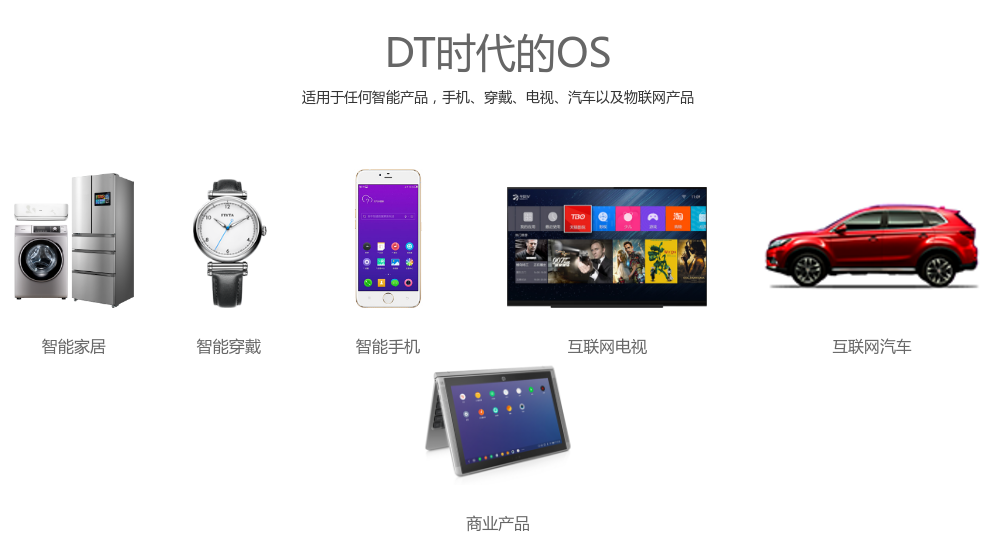
\includegraphics[width=0.6\textwidth]{figure/yunos.png}
    & 优秀程序员必不可少的基础知识
    && 加深对操作系统的理解,有利于深入编程;用户为了开发应用程序必须与操作系统打交道
    && 编程时借鉴操作系统的设计思想和算法(比如插件开发、微内核)
    && 设计操作系统或者修改现有的系统
    && Switch 和 If,哪个效率更高?
  \end{easylist}
\end{frame}

\begin{frame}[fragile]{为什么学习操作系统(2)}
  \begin{easylist}
    & 理解操作系统原理是掌握某些知识的必备基础,如大数据、云计算、分布式、WebService...
    & 操作系统中所用的许多概念和技巧可以推广应用到其他领域(如先来先服务、短作业
    优先…)
    & 可以提高情商 :)
	  \begin{tcolorbox}[colback=green!5,colframe=green!50,title=What's the meaning?]
		me\@me-desktop:~\$ chmod 700 myfate \\
		  Permission denied 
	  \end{tcolorbox}

%    \begin{block}{What's the meaning?}
%      me\@me-desktop:~\$ chmod 700 myfate \\
%      Permission denied 
%    \end{block}
  \end{easylist}
\end{frame}


\begin{frame}[fragile]{操作系统涉及的领域}
  \begin{easylist} \easyitem
    & 计算机体系结构/硬件
    & 软件设计
    & 程序设计语言
    & 数据结构
    & 算法
    & 网络
  \end{easylist}
  学习核心技术并能在其他地方应用

  操作系统是目前最复杂的软件系统
\end{frame}


\begin{frame}[fragile]{如何学好本课程}
  \begin{easylist} \easyitem
    & 理论学习
    & 实验、实习
    & 源代码分析、参与(Linux)
    & 多读相关书籍
  \end{easylist}
\end{frame}


\begin{frame}[fragile]{参考书目}
  \begin{easylist} \easyitem
    & 汤子瀛等,《计算机操作系统》,西安电子科技大学 ✿✿✿✿
    && 附带学习指导与题解
    & 孙钟秀,《操作系统教程》第三版,高等教育出版社
    & 操作系统精髓与设计原理
    & Silberschatz,《操作系统概念》(中、英文)第六版,高等教育出版社
  \end{easylist}
\end{frame}


\begin{frame}[fragile]{推荐阅读}
  \begin{easylist} \easyitem
    & 深入理解计算机系统,机械工业出版社  ✿✿✿✿✿
    & 操作系统之哲学原理✿✿✿
    & 鸟哥的Linux私房菜
    & 深入理解计算机系统
  \end{easylist}
\end{frame}


\begin{frame}[fragile]{考核方式}
  \begin{easylist} \easyitem 
    & 考核形式:
    && 闭卷+A4总结内容
    & 问题交流:
    && 课间
    && 电子邮件 
    && 办公室311/9:00AM---11:00AM, Monday
  \end{easylist}
\end{frame}


\begin{frame}[fragile]{讨论时间}
  \begin{easylist} \easyitem
    & 如果让你设计一个操作系统:
    && 你想到的功能都有哪些?请列举主要方面。
    && 你觉得未来的操作系统会往哪些方面发展/你最期待的功能是什么?
  \end{easylist}
\end{frame}

\subsection{1.1 操作系统的目标和作用}
\begin{frame}[fragile]{1.1 操作系统的目标和作用}
  \begin{easylist} \easyitem

  \end{easylist}
\end{frame}



\begin{frame}[fragile]{1.1.1 操作系统的目标}
  \begin{easylist} \easyitem
    & 方便性
    & 有效性
    & 可扩展性
    & 开放性
  \end{easylist}
\end{frame}


\begin{frame}[fragile]{1.1.2 操作系统的作用}
  \begin{easylist} \easyitem
    & (1) OS作为用户与计算机硬件系统之间的接口
    && 语音、视频接口
    && 图形用户接口
    && 命令接口
    && 系统调用接口
  \end{easylist}
  \begin{center}
    \begin{tikzpicture}[box/.style={draw,minimum height=0.7cm}]
      \draw[] node[box, minimum width=8cm] (hardware) {计算机硬件}
      node[box, minimum width=7cm, fill=red!10, align=center, above=0 of hardware] (os) {操作系统}
      node[box, above=0 of os, minimum width=2cm, xshift=-2cm] (sc) {系统调用}
      node[box, right=0 of sc] (cmd) {命令}
      node[box, right=0 of cmd] (gui) {窗口} 
      node[box, right=0 of gui] (voice) {语音、视频...} ;

      \draw[] node[box, above=0 of sc, minimum width=2cm] (app) {应用程序} ;
      \draw[] node[box, above=0 of app, minimum width=6cm, xshift=2cm] (user) {用户};
      \draw[latex-latex, very thick] ++(user.south) ++(-0,0)--++(0,-0.7);
      \draw[latex-latex, very thick] ++(user.south) ++(1.5,0)--++(0,-0.7);
    \end{tikzpicture}
  \end{center}
\end{frame}

\begin{frame}[fragile]
  \frametitle{iPhone X ditches Touch ID for Face ID\footnote{\url{https://venturebeat.com/2017/09/12/iphone-x-ditches-touch-id-for-face-id/}}}
  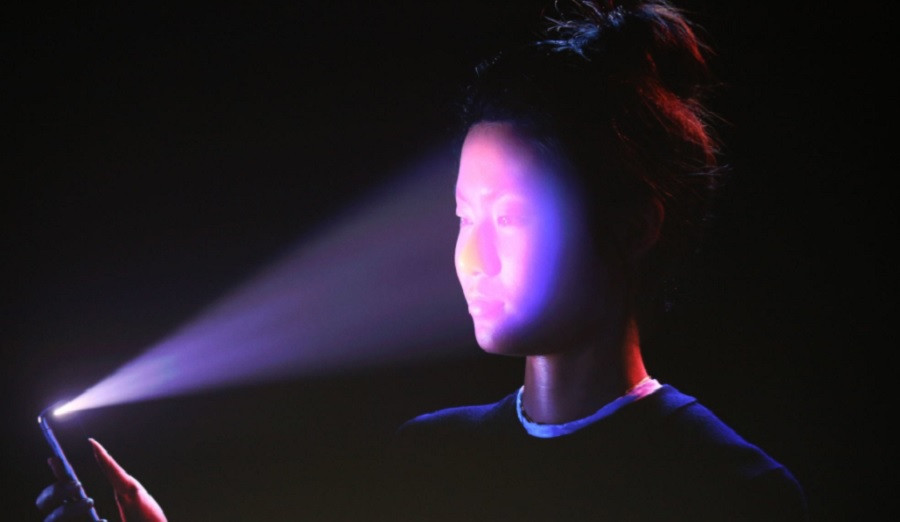
\includegraphics[width=0.85\textwidth]{figure/intro_face_id.jpg} 
\end{frame}


\begin{frame}[fragile]{1.1.2 操作系统的作用}
  \begin{easylist} \easyitem
    & (2) OS作为计算机系统资源的管理者
    && 处理机管理,用于分配和控制处理机;
    && 存储器管理,主要负责内存的分配与回收;
    && I/O设备管理,负责I/O设备的分配与操纵;
    && 文件管理,负责文件的存取、共享和保护。
  \end{easylist}
\end{frame}


\begin{frame}[fragile]{1.1.2 操作系统的作用}
  \begin{easylist} \easyitem
    & (3) OS用作扩充机器
    && 通常把覆盖了软件的机器称为扩充机器(Extended Machine)或虚机器(Virtual Machine)
  \end{easylist}
\end{frame}


\begin{frame}[fragile]{操作系统:魔幻家与管理者}
  \begin{easylist} \easyitem
    & 魔幻家
    && 差的东西变好:不用直接与硬件指令打交道,如磁盘的控制管理
    && 少得东西变多:虚拟内存
    && 无中生有:如逻辑盘
    & 管理者
    && CPU管理
    && 内存管理
    && 外存管理
    && IO管理
  \end{easylist}
\end{frame}


\begin{frame}[fragile]{1.1.3 推动OS发展的主要动力}
  \begin{easylist} \easyitem
    & 不断提高计算机资源利用率
    & 方便用户
    & 器件的不断更新换代
    & 计算机体系结构的不断发展
    & 操作系统的攻击与防范
    && 病毒和木马在一定程度上促进了操作系统的发展
    & 其他:
    && 价格、可靠性等
  \end{easylist}
\end{frame}



\begin{frame}[fragile]{硬件成本的不断下降举例}
  \begin{easylist} \easyitem
    & IBM制造的第一张硬盘RAMAC 350(1956/9/4),容量只有5M,重达一吨,需要一家飞机来运。
    & 硬件成本的下降使得操作系统可以变得更为复杂,使操作系统从最初的几百行代码、
    几千行代码变为4000万行代码的复杂系统(Windows XP),Linux 2.6.7内核超过1000万行
  \end{easylist}
  \centering
  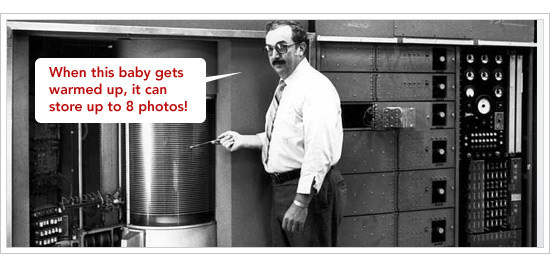
\includegraphics[width=0.7\textwidth]{figure/intro_first_disk2.jpg}
  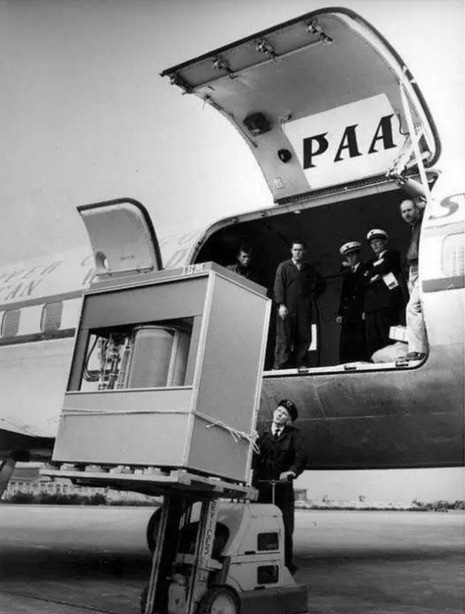
\includegraphics[width=0.25\textwidth]{figure/intro_first_disk1.jpg}
\end{frame}

\subsection{1.2 操作系统的发展历程}
\begin{frame}[fragile]{1.2 操作系统的发展历程}
  \begin{easylist} \easyitem
    & 状态机操作系统(1940年以前)
    & 单一操作员单一控制终端(20世纪40年代)
    & 批处理操作系统
    && UMES
    & 多道批处理操作系统
    && OS/360
    & 分时系统
    && Unix
    & 实时操作系统
    & 现代操作系统
  \end{easylist}
\end{frame}


\begin{frame}[fragile]{1.2.1 第一代计算机(手工操作阶段)}
  \begin{easylist} \easyitem
    & 1. 完全人工操作方式
    && 缺点:
    &&& 用户独占全机
    &&& CPU等待人工操作
    & 2. 脱机输入/输出(Off-Line I/O)方式
  \end{easylist}
\end{frame}


\begin{frame}[fragile]{脱机输入/输出示例}
  \begin{center}
    \begin{tikzpicture}[box/.style={draw, align=center,minimum height=1cm,minimum width=2.cm, fill=yellow!10},
      database/.style={ cylinder, cylinder uses custom fill,
        fill=green!2, align=center, shape border rotate=90, aspect=0.15,
        inner sep=0.2cm, minimum width=2.cm, minimum height=1cm, draw},
      multidocument/.style={
        shape=tape,
        draw,
        fill=gray!5,
        tape bend top=none,
        minimum height=1cm,
        minimum width=2.cm,},
      link/.style={draw, thick,-{Latex[scale=1.2]}},
      scale=0.6]
      \draw node[multidocument] (input) {输入设备}
      node[box,right=of input] (w1) {外围机}
      node[database,right=of w1](disk1) {磁盘} ;
      \draw[link] (input)--(w1);
      \draw[link] (w1)--(disk1);

      \draw node[database, below=of input, very thick, draw=red!60] (disk2) {磁盘}
      node[box,right=of disk2, very thick, draw=red!60] (main) {主机}
      node[database,right=of main, very thick, draw=red!60] (disk3) {磁盘} ;
      \draw[link] (disk2)--(main);
      \draw[link] (main)--(disk3);

      \draw node[database, below=of disk2] (disk4) {磁盘}
      node[box,right=of disk4] (w2) {外围机}
      node[multidocument,right=of w2] (output) {输出设备} ;
      \draw[link] (disk4)--(w2);
      \draw[link] (w2)--(output);
    \end{tikzpicture}
  \end{center}
  \begin{easylist} \easyitem
    & 优点:
    && 减少了CPU的空闲时间。
    && 提高了I/O速度。
  \end{easylist}
\end{frame}




\begin{frame}[fragile]{1.2.2 单道批处理系统}
  \begin{easylist} \easyitem
    & 单道批处理系统(Simple Batch Processing System)的处理过程
    & 单道程序运行情况
    && 特征:(1)自动性; (2)顺序性; (3) 单道性
  \end{easylist}
  \begin{center}
\scalebox{0.77}{
    \begin{tikzpicture}[tip/.style={ minimum height=1cm,minimum width=2.cm}]
      \draw node[tip] (user) {用户程序} node[tip, below=0.2cm of user] (jiandu) {监督程序}  node[tip, below=0.2cm of jiandu] (io) {I/O操作};

      \draw node[tip, right=of user, ] (jisuan) {计算}
      node[tip,right=0 of jisuan] (input) {请求输入}
      node[tip, right=0 of input] (b14){}
      node[tip, right=0 of b14] (b15){}
      node[tip, right=0 of b15, ] (b16) {继续计算} ;

      \draw node[tip, right=of jiandu] (b22){}
      node[tip, right=0 of b22] (b23) {启动I/O}
      node[tip, right=0 of b23] (b24) {}
      node[tip, right=0 of b24] (b25) {I/O完成};

      \draw node[tip, right=of io] (b32){}
      node[tip, right=0 of b32] (b33) {}
      node[tip, right=0 of b33] (b34) {}
      node[tip, right=0 of b34] (b35) {结束中断};

      \draw[draw=blue!60,line width=2pt] (2, -0.5)--(4,-0.5) (4,-1.7)--(6,-1.7) (6,-2.9)--(8,-2.9)  (8,-1.7)--(10,-1.7) (10,-0.5)--(12,-0.5);
      \draw[dashed] (4,-0.5)--(4,-1.6) (6,-1.7)--(6, -2.9) (8, -1.7)--(8, -2.9) (10,-0.5)--(10,-1.6);
    \end{tikzpicture}
}
  \end{center}
\end{frame}


\begin{frame}[fragile]{单道批处理系统示例}
  \begin{center}
    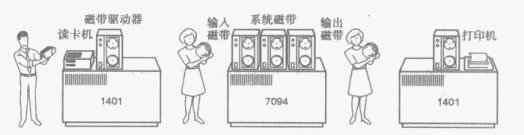
\includegraphics[width=0.9\textwidth]{figure/intro-batch_os.jpg}
  \end{center}
\end{frame}


\begin{frame}[fragile]{密歇根执行系统UMES}
  \begin{easylist} \easyitem
    & MAD/UMES
    && R.M.Graham, Bruce Arden, Bernard Galler
    && 密歇根算法译码器/密歇根大学执行系统
  \end{easylist}

  \begin{columns}[onlytextwidth]
    \begin{column}{0.5\textwidth}
      \centering
      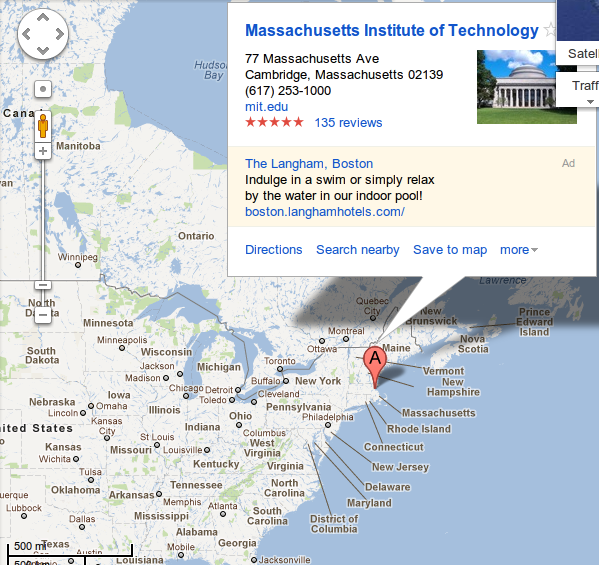
\includegraphics[width=0.9\textwidth]{figure/intro-mit_location.jpg}
    \end{column}
    \begin{column}{0.5\textwidth}
      \centering
      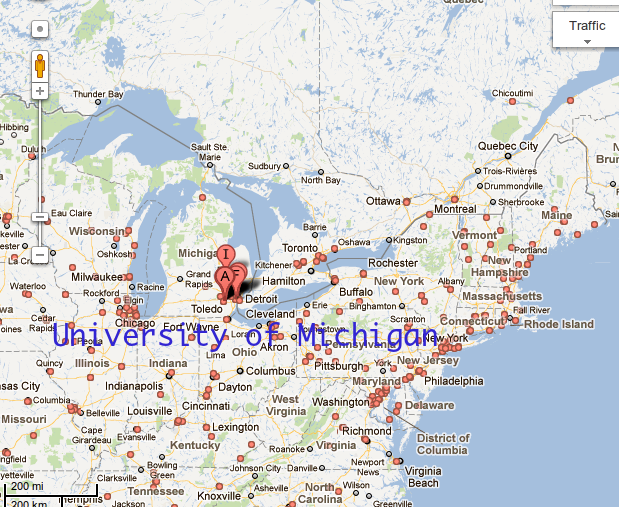
\includegraphics[width=0.9\textwidth]{figure/intro-michigan_location.jpg}
    \end{column}
  \end{columns}
\end{frame}



\begin{frame}[fragile]{1.2.3 多道批处理系统}
  \begin{easylist} \easyitem
    & 多道批处理系统运行过程示例
  \end{easylist}
  \centering
  \begin{tikzpicture}[tip/.style={ minimum height=1cm,minimum width=2.cm},
    box/.style={draw, minimum height=0.8cm,minimum width=1.5cm},
    line/.style={very thick, draw=blue!50}
    ]

    \draw[] node[tip] (a) {程序A}
    node[tip,below=0.2cm of a] (b) {程序B}
    node[tip,below=0.2cm of b] (c) {程序C}
    node[tip,below=0.2cm of c] (d) {程序D}
    node[tip,below=0.2cm of d] (e) {处理器} ;

    \draw[] node[box, right=0 of a] {运行} node[box, right=7.5cm of a] {运行};
    \draw[line] (0.8,-0.45)--(10.5,-0.45);

    \draw[] node[box, right=3cm of b] {运行} node[box, right=6cm of b] {运行};
    \draw[line] (0.8,-1.65)--(10.5,-1.65);

    \draw[] node[box, right=4.5cm of c] {运行};
    \draw[line] (0.8,-2.85)--(10.5,-2.85);

    \draw[] node[box, right=1.5cm of d] {运行};
    \draw[line] (0.8,-4.1)--(10.5,-4.1);

    \draw[] node[box, right=0 of e] (e2) {运行}
    node[box, right=0 of e2] (e3) {运行}
    node[box, right=0 of e3] (e4) {运行}
    node[box, right=0 of e4] (e5) {运行}
    node[box, right=0 of e5] (e6) {运行}
    node[box, right=0 of e6] (e7) {运行};
    \draw[line, draw=red!60] (0.8,-5.3)--(10.5,-5.3);

    \draw[line, -Latex] (2,-6)--(8,-6) node[right] {时间};
  \end{tikzpicture}
\end{frame}


\begin{frame}[fragile]{多道批处理系统}
  \begin{easylist} \easyitem
    & 特征
    && 多道性
    && 无序性
    && 调度性
  \end{easylist}
\end{frame}


\begin{frame}[fragile]{多道批处理系}
  \begin{easylist} \easyitem
    & 优缺点
    && 资源利用率高
    && 系统吞吐量大
    && 平均周转时间长
    && 无交互能力
  \end{easylist}
\end{frame}


\begin{frame}[fragile]{多道批处理系统}
  \begin{easylist} \easyitem
    & 需要解决的问题
    && 处理机管理问题
    && 内存管理问题
    && I/O设备管理问题
    && 文件管理问题
    && 作业管理问题
  \end{easylist}
\end{frame}


\begin{frame}[fragile]{代表OS}
  \begin{easylist} \easyitem
    & IBM OS/360
    && 运行于IMB System 360、370、4300
    && 引入了内存的分段管理
  \end{easylist}
\end{frame}


\begin{frame}[fragile]{操作系统的定义}
  一组控制和管理计算机硬件和软件资源、合理地对各类作业进行调度、以及方便用户的程序的集合
\end{frame}


\begin{frame}[fragile]{操作系统的定义}
  \begin{easylist} \easyitem
    & 说明
    && 操作系统是软件,是系统软件,是由一整套程序组成。
    && 基本职能:控制和管理系统内各种资源,有效地组织多道程序地运行
    && 提供众多服务,方便用户使用,扩充硬件功能。
    && 操作系统的地位:其他软件的支撑环境
  \end{easylist}
\end{frame}


\begin{frame}[fragile]{1.2.4 分时系统}
  \begin{easylist} \easyitem
    & 1. 分时系统(Time-Sharing System)的产生
    && 用户的需求具体表现在以下几个方面:
    && (1) 人—机交互
    && (2) 共享主机
    && (3) 便于用户上机
  \end{easylist}
\end{frame}


\begin{frame}[fragile]{1.2.4 分时系统}
  \begin{easylist} \easyitem
    & 2. 分时系统实现中的关键问题
    && (1) 及时接收
    && (2) 及时处理
  \end{easylist}
\end{frame}


\begin{frame}[fragile]{1.2.4 分时系统}
  \begin{easylist} \easyitem
    & 3. 分时系统的特征
    && (1)多路性。(宏观:多用户同时工作,共享系统资源;微观:用户作业轮流运行 )
    && (2) 独立性
    && (3) 及时性
    && (4) 交互性
  \end{easylist}
\end{frame}


\begin{frame}[fragile]{代表性OS}
  \begin{easylist} \easyitem
    & Multics、Unix
    && 密歇根的R.M.Graham主持,MIT、DEC、贝尔实验室
    && 贝尔实验室 $\Rightarrow$ 单干 $\Rightarrow$ Unix $\Rightarrow$ 图灵奖
    && MIT $\Rightarrow$ 应用于商用领域的分时系统CTSS
  \end{easylist}
\end{frame}


\begin{frame}[fragile]{1.2.5 实时系统}
  \begin{easylist} \easyitem
    & 1. 应用需求
    && (1) 实时控制
    && (2) 实时信息需求
  \end{easylist}
\end{frame}

\begin{frame}[fragile]{1.2.5 实时系统}
  \begin{easylist} \easyitem
    & 2. 定义
    && 实时:
    &&& 指对随机发生的外部事件做出及时的相应并对其进行处理。(所谓事件是指来自与计算机系统相连接的设备所提出的服务要求和采集数据)
    && 实时系统:
    &&& 指系统能及时(或即时)响应外部事件的请求,在规定的时间内完成对该事件的处理,并控制所有实时任务协调一致地运行
  \end{easylist}
\end{frame}

\begin{frame}[fragile]{1.2.5 实时系统}
  \begin{easylist} \easyitem
    & 3. 实时任务
    && 1) 按任务执行时是否呈现周期性来划分
    &&& (1) 周期性实时任务
    &&& (2) 非周期性实时任务
    && 2) 根据对截止时间的要求来划分
    &&& (1) 硬实时任务(hard real-time task)
    &&& (2) 软实时任务(Soft real-time task)
  \end{easylist}
\end{frame}

\begin{frame}[fragile]{1.2.5 实时系统}
  \begin{easylist} \easyitem
    & 4.实时系统与分时系统特征的比较
    && (1) 多路性
    && (2) 独立性
    && (3) 及时性
    && (4) 交互性
    && (5) 可靠性
  \end{easylist}
\end{frame}


\begin{frame}[fragile]{现代操作系统}
  \begin{easylist} \easyitem
    & 受益于80年代后计算机工业的快速发展
    & 价格下降使得个人有能力独享计算机
    & 个人独享使得分时系统的某些功能不再需要,似乎又回到了早期的SOSC阶段的标准函数库方式
    & 分时的需求
    & 网络的需求
  \end{easylist}
\end{frame}


\begin{frame}[fragile]{操作系统的演变}
\begin{center}
  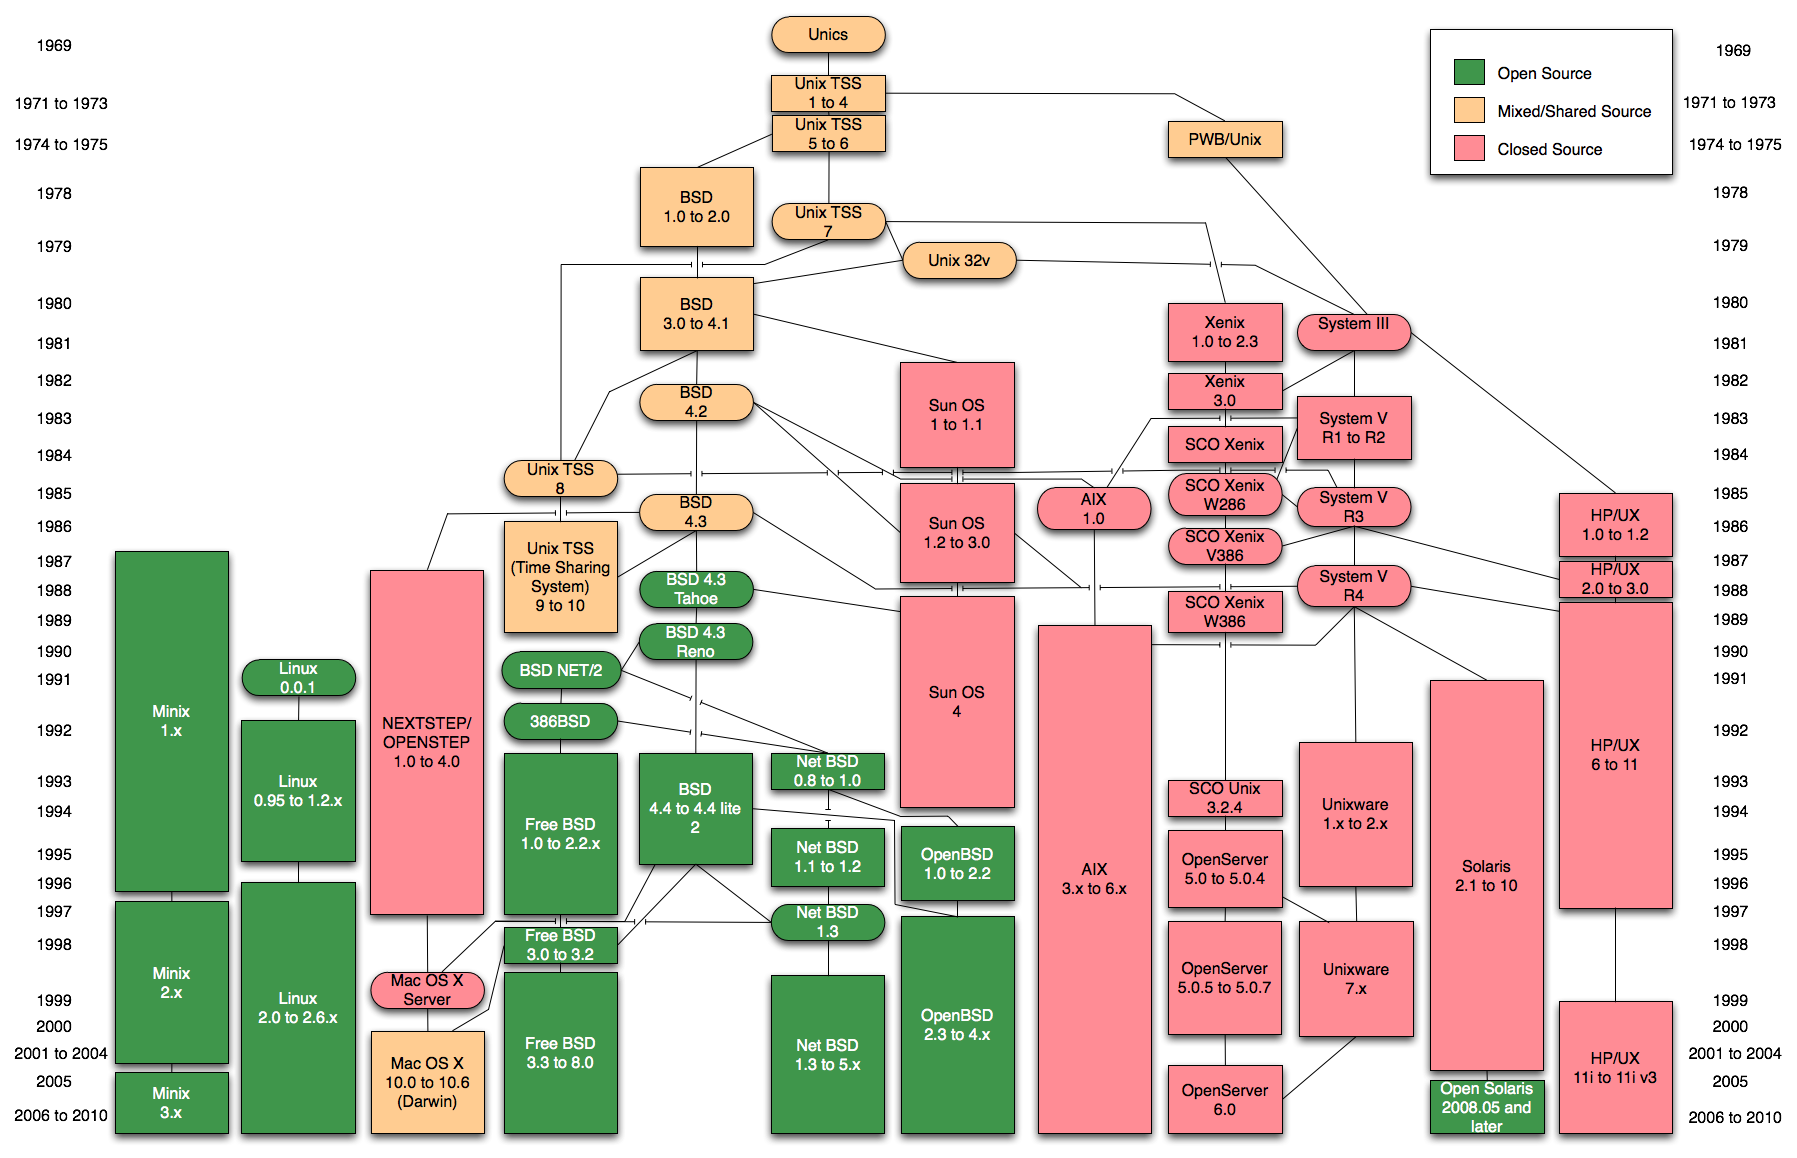
\includegraphics[width=0.9\textwidth]{figure/intro-unix_history-simple.png}
\end{center}
\end{frame}


\begin{frame}[fragile]{补充:计算机发展史}
  \begin{easylist}
    & 微型电脑就是一部缩小了的小型机 \footnote{https://www.zhihu.com/question/49073893}
  \end{easylist}

  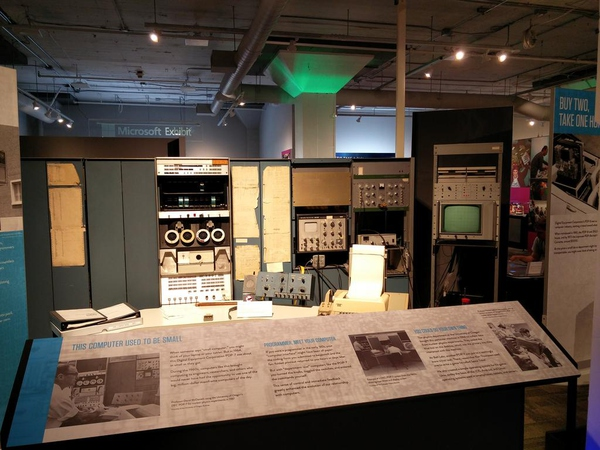
\includegraphics[width=0.9\textwidth]{figure/intro-minicomputer.jpg}
\end{frame}

\begin{frame}[fragile]{控制台tty}
  \begin{easylist}
    & 在类Unix里,键盘显示器,都是虚拟的teletypewriter
    & 真正的teletypewriter长这样
  \end{easylist}
  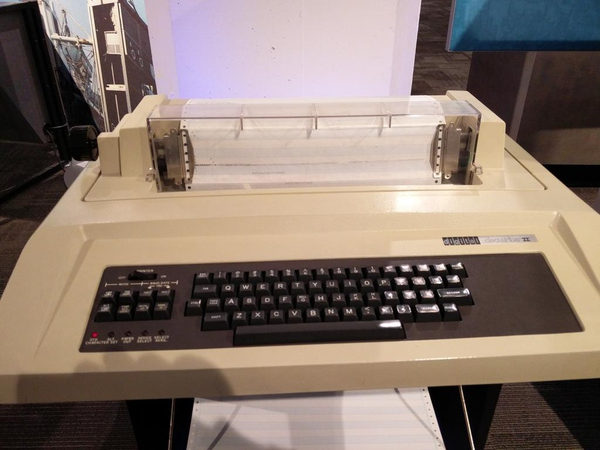
\includegraphics[width=0.9\textwidth]{figure/intro-tty.jpg}
\end{frame}

\begin{frame}[fragile]{tar命令解压缩}
  \begin{easylist}
    & 为什么解压缩往往会用到tar -zxvf?这个tar命令究竟是什么?
    & 实物版的tar长这样,叫Tape Archive
  \end{easylist}
  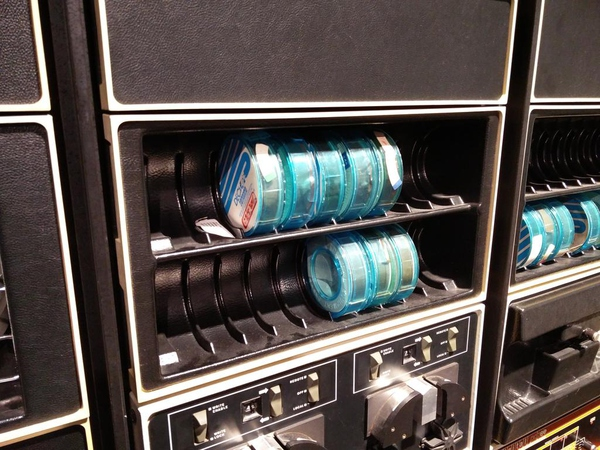
\includegraphics[width=0.9\textwidth]{figure/intro-tar.jpg}
\end{frame}

\begin{frame}[fragile]{为什么硬盘要mount/umount}
  \begin{easylist}
    & 硬盘都是固定在电脑里的,mount管什么用?这货叫DEC Pack,就是数据库图标里的那个圆柱,要让这圆柱(硬盘)工作起来,先得把它放进硬盘驱动器,这个驱动器就叫/dev/hda(也可能是hdb,看一共有几个Hard Drive)。
  \end{easylist}
  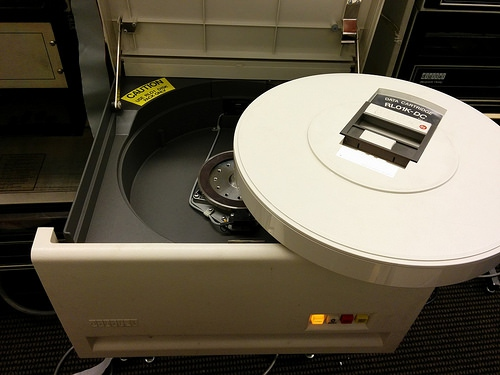
\includegraphics[width=0.9\textwidth]{figure/intro-mount.jpg}
\end{frame}

\begin{frame}[fragile]{结论}
  \begin{easylist}
    & 计算机的原理都是一样的,只是尺寸变小后这些部分{\color{red}看起来}像是一体
    的。
    & 课外阅读:带你逛西雅图活电脑博物馆
  \end{easylist}
\end{frame}

\begin{frame}[fragile]{操作系统的“差不多”精神}
  \begin{easylist} \easyitem
    & 与数学相比软件学科具有“差不多”特点
    && 数学家与软件专家的故事
    && 差不多:如“算法复杂度”
  \end{easylist}
\end{frame}

\subsection{1.3 操作系统的四个基本特征}
\begin{frame}[fragile]{1.3 操作系统的四个基本特征}
  \begin{easylist} \easyitem
    & 并发(Concurrence)
    & 共享(Sharing)
    & 虚拟(Virtual)
    & 异步性(Asynchronism)
  \end{easylist}
\end{frame}


\begin{frame}[fragile]{1.3.1 并发}
  \begin{easylist} \easyitem
    & 并行性:
    && 是指两个或多个事件在同一时刻发生;
    & 并发性:
    && 是指两个或多个事件在同一时间间隔内发生。
  \end{easylist}
  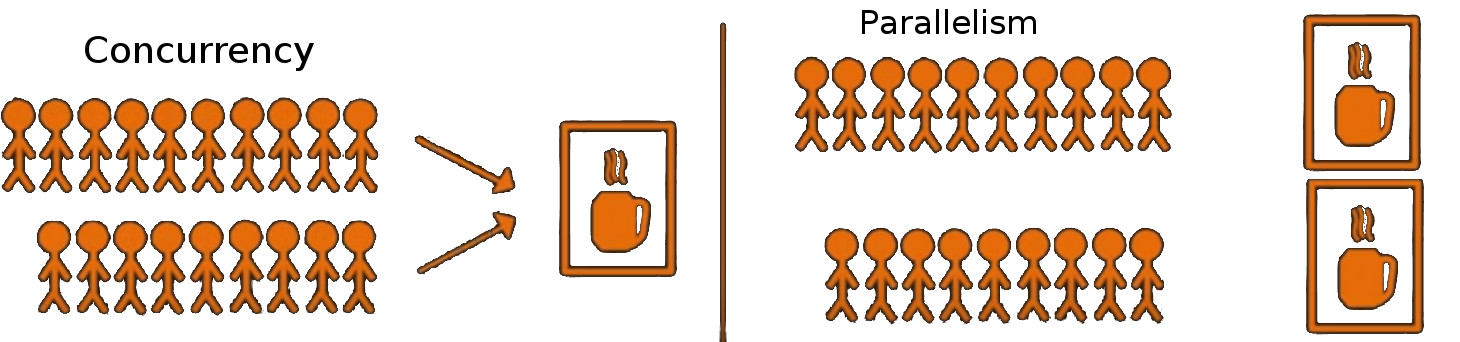
\includegraphics[width=0.9\textwidth]{figure/parallel.jpg}
\end{frame}


\begin{frame}[fragile]{1.3.2 共享}
  \begin{easylist} \easyitem
    & 互斥共享方式
    & 同时访问方式

    & 例如:
    && 三个程序在同一时间间隔内访问磁盘
    && 多个程序在同一时间间隔内要求打印文本
  \end{easylist}
\end{frame}


\begin{frame}[fragile]{1.3.3 虚拟}
  \begin{easylist} \easyitem
    & “虚拟”:是指通过某种技术把一个物理实体变为若干个逻辑上的对应物。相应地,用于实现虚拟的技术,称为虚拟技术。
  \end{easylist}
\end{frame}


\begin{frame}[fragile]{1.3.4 异步性}
  \begin{easylist} \easyitem
    & 假设能同时双击两个大小相同的Word文档,你能断定哪一个先打开吗?
    & 进程是以人们不可预知的速度向前推进,此即进程的异步性
  \end{easylist}
\end{frame}


\subsection{1.4 操作系统的主要功能}
\begin{frame}[fragile]{1.4 操作系统的主要功能}
  \begin{easylist} \easyitem
    & 1.4.1 处理机管理
    && (1) 进程控制
    && (2) 进程同步
    &&& ① 进程互斥方式:诸进程(线程)在对临界资源进行访问时,应采用互斥方式;
    &&& ② 进程同步方式:指在相互合作去完成共同任务的诸进程(线程)间,由同步机构对它们的执行次序加以协调。
    && (3) 进程通信
    && (4) 调度
  \end{easylist}
\end{frame}


\begin{frame}[fragile]{1.4.2 存储器管理}
  \begin{easylist} \easyitem
    & 1. 内存分配
    && 分配方式:
    &&& 静态分配方式、动态分配方式
    && 在内存分配的机制中应具有这样的结构和功能:
    &&& ① 内存分配数据结构
    &&& ② 内存分配功能
    &&& ③ 内存回收功能
  \end{easylist}
\end{frame}


\begin{frame}[fragile]{1.4.2 存储器管理}
  \begin{easylist} \easyitem
    & 2. 内存保护
    && 确保每道用户程序都只在自己的内存空间内运行,彼此互不干扰。
  \end{easylist}
\end{frame}


\begin{frame}[fragile]{1.4.2 存储器管理}
  \begin{easylist} \easyitem
    & 3. 地址映射
    && “逻辑地址”或“相对地址”。
    && “物理地址”
  \end{easylist}
\end{frame}


\begin{frame}[fragile]{1.4.2 存储器管理}
  \begin{easylist} \easyitem
    & 4. 内存扩充
    && 借助于虚拟存储技术,从逻辑上去扩充内存容量
    && 为了能在逻辑上扩充内存,系统必须具有内存扩充机制, 用于实现下述各功能:
    &&&  (1) 请求调入功能
    &&& (2) 置换功能
  \end{easylist}
\end{frame}


\begin{frame}[fragile]{1.4.3 设备管理}
  \begin{easylist} \easyitem
    & 缓冲管理
    & 设备分配和设备处理
    & 虚拟设备等功能。
  \end{easylist}
\end{frame}


\begin{frame}[fragile]{1.4.4 文件管理}
  \begin{easylist} \easyitem
    & 1. 文件存储空间的管理
    && 相应的数据结构,存储空间的分配和回收功能。
    && 通常是采用离散分配方式,以减少外存零头,并以盘块为基本分配单位。盘块的大小通常为512 B\~8 KB。
    & 2. 目录管理
    & 3. 文件的读写管理与保护
  \end{easylist}
\end{frame}


\begin{frame}[fragile]{1.4.5 用户接口}
  \begin{easylist} \easyitem
    & 1. 系统调用
    & 2. 壳(Shell)
    && 命令,如Linux Shell,可运行多个
    && 图形,如Windows Explorer,保持一个实例
    \vspace{1cm}
    & 示例演示
  \end{easylist}
\end{frame}


\begin{frame}[fragile]{1.5 操作系统的结构设计}
  \begin{easylist} \easyitem
    & 1. 无结构操作系统
    & 2. 模块化OS结构
    & 3. 分层式OS结构
  \end{easylist}
\end{frame}

\begin{frame}[fragile]{微内核操作系统结构}
  \begin{easylist} \easyitem
    & 1. 客户/服务器模式(Client-Server Model)
    & 2. 面向对象的程序设计技术(Object-Orientated Programming)
    & 3. 微内核技术
    && 微内核所提供的功能,通常都是一些最基本的功能,如进程管理、存储器管理、进程间通信、 低级I/O功能。
  \end{easylist}
\end{frame}


\begin{frame}[fragile]{CH1 END}
  \begin{easylist} \easyitem
    & 调查作业
    && 操作系统对小米的影响(第1次作业)
    && Shell, Terminal和Console的区别是什么?(第2次作业)

    % https://www.zhihu.com/question/20388511
    % http://superuser.com/questions/144666/what-is-the-difference-between-shell-console-and-terminal
  \end{easylist}

  助教:
  鲁国轩: rt\_lgx@163.com
  
\end{frame}

%%% Local Variables:
%%% mode: latex
%%% TeX-master: "../os"
%%% End:

%\section{进程管理}

\begin{frame}[fragile]{CH2 进程管理}
  \begin{easylist} \easyitem
    & 2.1 进程的基本概念
    & 2.2 进程控制
    & 2.3 进程同步
    & 2.4 经典进程同步问题
    & 2.5 管程机制
    & 2.6 进程通信
    & 2.7 线程
  \end{easylist}
\end{frame}


\subsection{2.1 进程的基本概念}
\begin{frame}[fragile]{2.1 进程的基本概念}
  \begin{easylist} \easyitem
    & 未配置OS的系统:程序顺序执行
    && 程序的顺序执行及其特征
    & 现代多道程序环境下:程序并发执行
    && 程序的并发执行及其特征
  \end{easylist}
\end{frame}


\begin{frame}[fragile]{2.1 进程的基本概念}
  \begin{easylist} \easyitem
    & 2.1.1  程序的顺序执行及特征
    && 1. 程序执行有固定的时序
    \begin{center}
      \scalebox{0.7}{
        \begin{tikzpicture}[c/.style={draw,circle, thick, minimum height=0.5cm}]
          \draw[] node[c] (i1) {$I_1$}
          node[c, right=of i1] (c1) {$C_1$}
          node[c, right=of c1] (p1) {$P_1$}
          node[c, right=of p1] (i2) {$I_2$}
          node[c, right=of i2] (c2) {$C_2$}
          node[c, right=of c2] (p2) {$P_2$};
          \path[-Latex] (i1) edge (c1) (c1) edge (p1) (p1) edge (i2) (i2) edge (c2) (c2) edge (p2);
        \end{tikzpicture}
      }
    \end{center}

    && 2. 程序顺序执行时的特征
    &&& 顺序性:操作的前后依赖性
    &&& 封闭型:独占资源,资源状态只有本程序更改
    &&& 可再现性:初始环境和条件,结果相同
  \end{easylist}
\end{frame}


\begin{frame}[fragile]{程序顺序执行的优点}
  \begin{easylist} \easyitem
    & 符合人的直觉
    & 有利于错误调试
    && DEMO
    && BUG vs DEBUG
  \end{easylist}
  \begin{columns}[onlytextwidth,T]
    \begin{column}{0.5\textwidth}
      \begin{block}{\small 格蕾丝·赫柏(Grace Murray Hopper)}
        \scriptsize
        赫柏是一位为美国海军工作的电脑专家。1945年的一天,赫柏对Harvard Mark II设置好17000个继电器进行编程后,技术人员在进行整机运行时,它突然停止了工作。于是他们爬上去找原因,发现这台巨大的计算机内部一组继电器的触点之间有一只飞蛾,这显然是由于飞蛾受光和热的吸引,飞到了触点上,然后被高电压击死。所以在报告中,赫柏用胶条贴上飞蛾,并把“bug”来表示"一个在电脑程序里的错误"。
      \end{block}
    \end{column}
    \begin{column}{0.45\textwidth}
      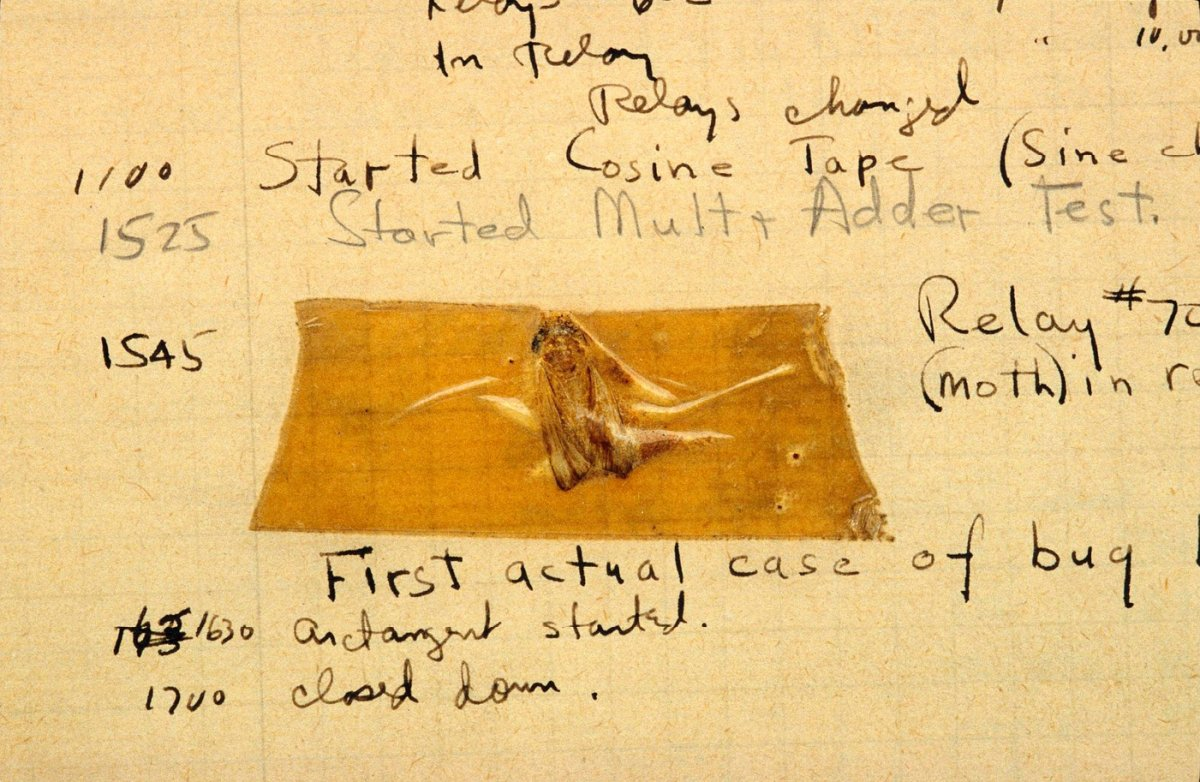
\includegraphics[width=0.85\textwidth]{figure/bug.jpg}
    \end{column}
  \end{columns}
\end{frame}


\begin{frame}[fragile]{2.1.2 程序的并发执行}
  \begin{easylist} \easyitem
    & 特征
    && 间断性:
    &&& 如打印程序等待计算程序完成之后方可继续
    &&& 执行—暂停—执行……
    && 失去封闭性
    &&& 主要由共享资源引起,资源的状态将由多个程序改变;
    && 不可再现性
    &&& 计算结果与并发程序的执行速度有关
  \end{easylist}
\end{frame}


\begin{frame}[fragile]{例子 --- 课堂讨论}
  \begin{easylist} \easyitem
    & 有2个循环程序$A$和$B$,共享一个变量$N$( 设$N$的初值为$n$ )
    & 程序$A$每执行一次时,都要做$N:=N+1$
    & 程序$B$每次要执行$Print(N)$, 然后再做$N:=0$
    \vspace{1cm}
    & 若程序$A$,$B$以不同的速度运行,其结果将会是?
    & 注意,代码采用了类Pascal语言
  \end{easylist}
\end{frame}


\begin{frame}[fragile]{例子}
  \begin{easylist} \easyitem
    & N:=N+1在print(N)和N:=0之前,则N值分别为n+1, n+1, 0.
    & N:=N+1在print(N)和N:=0之后,则N值分别为n, 0, 1.
    & N:=N+1在print(N)和N:=0之间,则N值分别为n, n+1, 0.
  \end{easylist}
\end{frame}


\begin{frame}[fragile]{Python代码示例}
  \begin{lstlisting}[keywordstyle=\color{red},basicstyle=\small, language=python]
from multiprocessing import Process
def f1(i):
    while i<10:
        i = i+1
    print 'f1 finished‘

def f2(i):
    while i>-10:
        i = i-1
    print 'f2 finished!'


if __name__=='__main__':
    Process(target=f1, args=(0,)).start()
    Process(target=f2, args=(0,)).start()
\end{lstlisting}
\end{frame}


\begin{frame}[fragile]{多次运行结果}
  \begin{easylist} \easyitem
    & Run 1:
    && f1 finished
    && f2 finished!
    & Run 2:
    && f1 finished
    && f2 finished!
    & Run 3:
    && f2 finished!
    && f1 finished
  \end{easylist}
\end{frame}


\begin{frame}[fragile]{思考}
  \begin{easylist} \easyitem
    & 在多道程序环境下,程序执行属于并发执行,具有3个典型特性(哪3个?)
    & 结果的不可再现性的问题
    & 要保证结果的再现性,就需要对并发执行的程序加以描述和控制,其结果就是引入了“进程”概念
    & 进程=程序+执行
    & 在Multics OS之前,主要采用IBM的“作业(job)”概念,之后,改为进程(Process)
  \end{easylist}
\end{frame}


\subsection{2.1.3 进程的特征和状态}
\begin{frame}[fragile]{2.1.3 进程的特征和状态}
  \begin{easylist} \easyitem
    & 进程的定义
    && 程序的一次执行过程
    && 进程是程序实体的执行过程,是系统进行资源分配与调度的独立单位。
  \end{easylist}
\end{frame}


\begin{frame}[fragile]{进程的特征}
  \begin{easylist} \easyitem
    & 1.结构特征
    && 进程:由程序段、数据段及进程控制块三部分构成,总称“进程映像(Unix中)”。
    & 2.动态性:进程实体的一次执行过程
    && 由“创建”而产生,由“调度”而执行;由得不到资源而阻塞;由撤消而消亡。(而程序是静态的)。
    & 3.并发性:只有建立了进程,才能并发执行
    && 如同时浏览多个网页
    & 4.独立性: 独立运行,独立获得资源。资源分配与调度的基本单位
    && 浏览器邮箱登陆实例
    & 5.异步性:
    && 各进程以不可预知的速度向前推进
    && 间断性
  \end{easylist}
\end{frame}


\begin{frame}[fragile]{进程的状态}
  \begin{easylist} \easyitem
    & 进程执行的间断性,使得进程具有多种不同的状态
    & 进程的三种基本状态
    && 就绪
    && 执行
    && 阻塞
  \end{easylist}
  \vspace*{-1cm}
  \centering
  \begin{figure}
    \begin{tikzpicture}[c/.style={draw,ellipse, thick, minimum height=0.5cm}]
      \draw[] node[c] (ready) {就绪}
      node[c, below left=of ready, xshift=-1cm] (block) {阻塞}
      node[c, fill=yellow!50, below right=of ready, yshift=-1cm] (exec) {执行};

      \path[->,thick] (block) edge[bend left=30] node[below right]{I/O完成} (ready)
      (exec) edge[bend left=30] node[below]{I/O请求} (block)
      (ready) edge[bend right=30] node[left]{进程调度} (exec)
      (exec) edge[bend right=30] node[right]{时间片完} (ready);
    \end{tikzpicture}
    \caption{进程的三种基本状态及其转换}
  \end{figure}
\end{frame}


\begin{frame}[fragile]{挂起状态(被换出内存的状态)}
  \begin{easylist} \easyitem
    & 引入原因
    && 终端用户请求
    && 父进程请求
    && 负荷调节需要
    && 操作系统需要
    & 挂起演示
    && vi,CTRL+z; debugging
    & 进程状态的转换
    && 活动就绪 $\Rightarrow$ 静止就绪
    && 活动阻塞 $\Rightarrow$ 静止阻塞
    && 静止就绪 $\Rightarrow$ 活动就绪
    && 静止阻塞 $\Rightarrow$ 活动阻塞
  \end{easylist}
\end{frame}


\begin{frame}[fragile]{具有挂起状态的进程状态图}
\centering
\begin{figure}
  \scalebox{0.8}{
    \begin{tikzpicture}[c/.style={draw,ellipse, thick, minimum height=1cm, minimum width=2cm}]
      \draw[] node[c, fill=yellow!50] (exec) {执行}
      node[c, below left=1.5cm of exec, yshift=-1cm] (ready1) {活动就绪}
      node[c, below right=1.5cm of exec, yshift=-1cm] (ready2) {静止就绪}
      node[c, below left=1cm of ready1, yshift=-1cm] (block1) {活动阻塞}
      node[c, below left=1cm of ready2, yshift=-1cm, xshift=1cm] (block2) {静止阻塞};

      \path[->,thick] (exec) edge[bend left=10] (ready1) (ready1) edge[bend left=15] (exec)
      (exec) edge[bend left=30] node[right]{挂起} (ready2)
      (ready1) edge[bend right=30] node[above]{挂起} (ready2)
      (ready2) edge[bend right=15] node[above]{激活} (ready1)
      (exec) edge[bend right=40] node{请求I/O} (block1)
      (block1) edge[bend right=30] node[above]{挂起} (block2)
      (block2) edge[bend right=15] node[above]{激活} (block1)
      (block2) edge[bend right=15] node[right]{释放} (ready2)
      (block1) edge[bend left=15] node[right]{释放} (ready1);
    \end{tikzpicture}
  }
  \caption{具有挂起状态的进程状态及其转换}
\end{figure}
\end{frame}


\begin{frame}[fragile]{实验}
  \begin{easylist} \easyitem
    & 写一个程序描述进程状态迁移过程。
    & 要求:
    && 提供导致进程状态变化的调用接口,包括创建、删除、调度、阻塞、时间到、挂起、激活等。
    && 实现进程列表显示的接口。
    && 注:这里设计的进程是一个假设的对象实体,是由程序自己创建和删除,不是系统维护的进程。
  \end{easylist}
\end{frame}




\subsection{进程控制块}
\begin{frame}[fragile]{2.1.4 进程控制块}
  \begin{columns}[onlytextwidth,T]
    \begin{column}{0.7\textwidth}
      \begin{enumerate}
      \item 进程控制块的作用
        \begin{itemize}
        \item 使不能独立运行的程序变为能独立运行的基本单位
        \item 是进程存在的唯一标志
        \item PCB (Process Control Block)常驻内存
        \end{itemize}
      \item 进程控制块中的信息
        \begin{itemize}
        \item 标识、处理机状态,进程调度信息,进程控制信息
        \end{itemize}
      \end{enumerate}
    \end{column}
    \begin{column}{0.3\textwidth}
      \begin{tabular}{|c|}
        \hline
        pid \\ \hline
        进程状态 \\ \hline
        现场  \\ \hline
        优先级  \\ \hline
        阻塞原因  \\ \hline
        程序地址  \\ \hline
        同步机制  \\ \hline
        资源清单  \\ \hline
        链接指针  \\ \hline
      \end{tabular}
    \end{column}
  \end{columns}
\end{frame}


\begin{frame}[fragile]{PCB}
  \begin{easylist} \easyitem
    & 进程标识符
    && 内部标识符与外部标识符(下页top示例)
    & 处理机状态
    && 能在断点恢复运行
    && 通用寄存器、指令计数器、程序状态字PSW、用户栈指针
    & 进程调度信息
    && 进程状态、优先级、与调度有关的其他信息(如等待时间)、事件(阻塞事件)
    & 进程控制信息
    && 程序和数据的地址
    && 进程同步和通信机制:消息队列指针、信号量
    && 资源清单
    && 在PCB队列中的链接指针
  \end{easylist}
\end{frame}

\begin{frame}[fragile]
  \frametitle{Linux top command}
  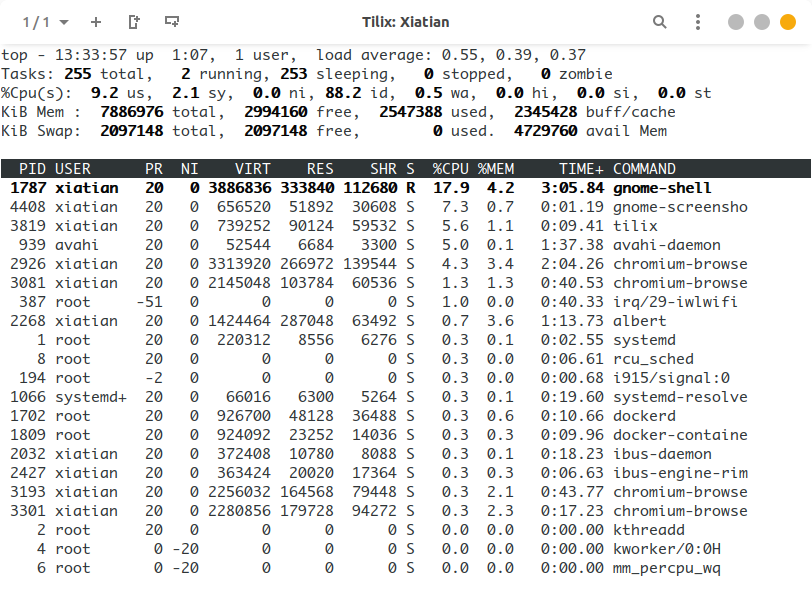
\includegraphics[width=0.9\textwidth]{figure/process-top.png}
\end{frame}



\begin{frame}[fragile]{PCB的组织: 链接方式}
  \centering
  \begin{figure}
    \scalebox{0.8}{
      \begin{tikzpicture}[q/.style={draw,thick, minimum height=0.8cm, minimum width=2.5cm},
        b/.style={draw, minimum width=1.5cm, minimum height=0.8cm}]
        \draw node[q] (exec) {执行指针} node[q, below=of exec] (ready) {就绪队列指针} node[q, below=of ready] (block) {阻塞队列指针} node[q, below=of block] (free) {空闲队列指针};

        \draw node[b, above right=3cm of exec, yshift=-1cm] (p1) {PCB1} node[b, right=0 of p1] (l1) {4};
        \draw node[b, below=0 of p1] (p2) {PCB2} node[b, right=0 of p2] (l2) {3};
        \draw node[b, below=0 of p2] (p3) {PCB3} node[b, right=0 of p3] (l3) {$\wedge$};
        \draw node[b, below=0 of p3] (p4) {PCB4} node[b, right=0 of p4] (l4) {8};
        \draw node[b, below=0 of p4] (p5) {PCB5} node[b, right=0 of p5] (l5) {$\wedge$};
        \draw node[b, below=0 of p5] (p6) {PCB6} node[b, right=0 of p6] (l6) {7};
        \draw node[b, below=0 of p6] (p7) {PCB7} node[b, right=0 of p7] (l7) {9};
        \draw node[b, below=0 of p7] (p8) {PCB8} node[b, right=0 of p8] (l8) {0};
        \draw node[b, below=0 of p8] (p9) {PCB9} node[b, right=0 of p9] (l9) {$\wedge$};
        \draw node[b, below=0 of p9] (p10) {$\cdots$} node[b, right=0 of p10] (l10) {$\cdots$};

        \path[->, thick] (l1.east) edge[draw=blue, to path={-- ++(1,0) |- (\tikztotarget)}] (l4.east);
        \path[->, thick] (l2.east) edge[draw=orange, to path={-- ++(0.5,0) |- (\tikztotarget)}] (l3.east);
        \path[->, thick] (l4.east) edge[draw=blue, to path={-- ++(0,-0.2)-- ++(1,0) |- (\tikztotarget)}] (l8.east);

        \path[->, thick] (l6.east) edge[draw=purple, to path={-- ++(0,-0.2)-- ++(0.5,0) |- (\tikztotarget)}] (l7.east);
        \path[->, thick] (l7.east) edge[draw=purple, to path={-- ++(0,-0.2)-- ++(0.5,0) |- (\tikztotarget)}] (l9.east);

        \draw[->, thick] (exec.east)--(p5.west);
        \draw[->, thick, draw=blue] (ready.east)--(p1.west);
        \draw[->, thick, draw=orange] (block.east)--(p2.west);
        \draw[->, thick, draw=purple] (free.east)--(p6.west);
      \end{tikzpicture}
    }
    \caption{PCB链接组织方式}
  \end{figure}
\end{frame}


\begin{frame}[fragile]{PCB的组织: 索引方式}
  \centering
  \begin{figure}
    \scalebox{0.8}{
      \begin{tikzpicture}[q/.style={draw,thick, minimum height=0.8cm, minimum width=2.5cm},
        a/.style={draw, -latex}]
        \draw node[q, fill=yellow!20] (exec) {执行指针} node[q, below=of exec] (ready) {就绪表指针} node[q, below=of ready] (block) {阻塞表指针};

        \draw node[q, minimum height=0.6cm, above right=of exec,yshift=-1cm] (rlist1) {} node[q, minimum height=0.6cm, below=0 of rlist1] (rlist2) {} node[q, minimum height=0.6cm, below=0 of rlist2] (rlist3) {} node[q, minimum height=0.6cm, below=0 of rlist3] (rlist4) {};

        \draw node[q, minimum height=0.6cm, below=of rlist4] (blist1) {} node[q, minimum height=0.6cm, below=0 of blist1] (blist2) {} node[q, minimum height=0.6cm, below=0 of blist2] (blist3) {} node[q, minimum height=0.6cm, below=0 of blist3] (blist4) {};

        \draw node[q, above right=1.5cm of rlist1, yshift=-1cm] (pcb1) {PCB1}
        node[q, below=0 of pcb1] (pcb2) {PCB2}
        node[q, below=0 of pcb2] (pcb3) {PCB3}
        node[q, below=0 of pcb3] (pcb4) {PCB4}
        node[q, below=0 of pcb4] (pcb5) {PCB5}
        node[q, below=0 of pcb5] (pcb6) {PCB6}
        node[q, below=0 of pcb6] (pcb7) {PCB7}
        node[q, below=0 of pcb7,draw=white] (pcb8) {$\cdots$};

        \path[a] (exec.east) edge[bend left=40] (pcb1.west);
        \draw[a] (ready.east)--(rlist1.west);
        \draw[a] (block.east)--(blist1.west);

        \draw[a] (rlist1.east)--(pcb3.west);
        \draw[a] (rlist2.east)--(pcb2.west);
        \draw[a] (rlist3.east)--(pcb4.west);

        \draw[a] (blist1.east)--(pcb7.west);
        \draw[a] (blist2.east)--(pcb6.west);
        \draw[a] (blist3.east)--(pcb5.west);
      \end{tikzpicture}
    }
    \caption{PCB索引组织方式}
  \end{figure}
\end{frame}

\begin{frame}[fragile]{补充}
  \begin{easylist} \easyitem
    & 指针和链表的概念
    && E.g.从链表中移除我的下一个:
    &&& 我的下一个是(变成)我的下一个的下一个
    && E.g. 从链表中移除我本身
    &&& 我的上一个的下一个是我的下一个

    & PCB和进程的代码数据放在一起吗?
    && 系统态和用户态
    && 系统空间和用户空间

    & 系统调用和普通调用的区别?
    && 系统调用会引起从用户态进入核心态
  \end{easylist}
\end{frame}

\begin{frame}[fragile]{Review last lesson}
  \begin{easylist} \easyitem
    & 什么是PCB,操作系统采用哪些方式对PCB进行组织和管理的?
  \end{easylist}
\end{frame}

\subsection{2.2 进程控制}
\begin{frame}[fragile]{2.2 进程控制}
  \begin{easylist} \easyitem
    & 2.2.1 进程的创建
    & 2.2.2 进程的终止
    & 2.2.3 进程的阻塞与唤醒
    & 2.2.4 进程的挂起与激活
  \end{easylist}
\end{frame}


\begin{frame}[fragile]{2.2.1 进程的创建}
  \begin{easylist} \easyitem
    & 进程图:
    & 引起创建进程的事件:
    & 进程的创建
  \end{easylist}
\end{frame}


\begin{frame}[fragile]{进程图}
  \begin{easylist} \easyitem
    && 描述了进程的家族关系
    && 子进程可继承父的资源,撤消时应归还给父进程,父的撤消会撤消全部子进程。
  \end{easylist}
\end{frame}


\begin{frame}[fragile]{引起创建进程的事件}
  \begin{easylist} \easyitem
    && 1.用户登录:
    &&& 为终端用户建立一进程
    && 2.作业调度:
    &&& 为被调度的作业建立进程
    && 3.提供服务:
    &&& 如要打印时建立打印进程
    && 4.应用请求:
    &&& 由应用程序建立多个进程
  \end{easylist}
\end{frame}


\begin{frame}[fragile]{进程的创建}
  \begin{easylist} \easyitem
    & (create原语)
    && 1.申请空白PCB(一个系统的PCB是有限的)
    && 2.为新进程分配资源(不同于一般的分配,PCB-LIST在一个特殊区域)
    && 3.初始化PCB
    && 4.将新进程插入就绪队列。
  \end{easylist}
\end{frame}


\begin{frame}[fragile]{2.2.2 进程的终止}
  \begin{easylist} \easyitem
    & 引起进程终止的事件
    & 进程的终止过程
  \end{easylist}
\end{frame}

\begin{frame}[fragile]{引起进程终止的事件}
  \begin{easylist} \easyitem
    & 1. 正常结束:如Halt、logoff
    & 2. 异常结束:如Protect error、overtime等
    & 3. 外界干预:
    && a. 系统员kill进程;(Linux演示)
    && b. 父进程终止;(impressive打开pdf文件演示)
    && c. 父进程请求。
  \end{easylist}
\end{frame}

\begin{frame}[fragile]{进程的终止过程}
  \begin{easylist} \easyitem
    & 1. 检查进程状态;
    & 2. 执行态$\rightarrow$中止,且置调度标志为真。
    & 3. 有无子孙需终止。
    & 4. 归还资源给其父进程或系统。
    & 5. 从PCB队列中移出PCB.
  \end{easylist}
\end{frame}



\begin{frame}[fragile]{2.2.3 进程的阻塞与唤醒}
  \begin{easylist} \easyitem
    & Content:
    && 引起进程阻塞和唤醒的事件
    && 进程阻塞过程
    && 进程唤醒过程
  \end{easylist}
\end{frame}

\begin{frame}[fragile]{引起进程阻塞和唤醒的事件}
  \begin{easylist} \easyitem
    & 1.请求系统服务而得不到满足时,如向系统请求打印。
    & 2.启动某种操作而需同步时:如该操作和请求该操作的进程需同步运行(即非异步操作)。
    & 3.新数据尚未到达:如进程A写,进程B读,则A未写完B不能读。
    & 4.无新工作可做。
  \end{easylist}
\end{frame}

\begin{frame}[fragile]{阻塞过程}
  \begin{easylist} \easyitem
    & 是进程自身的一种主动行为
    && a.调block原语
    && b.停止执行,修改PCB入阻塞队列(一个或多个),并转调度。
  \end{easylist}
\end{frame}

\begin{frame}[fragile]{唤醒过程}
  \begin{easylist} \easyitem
    & 其它相关进程完成。
    && a.wakeup原语
    && b.修改PCB,入就绪队列
    && 可见,有block原语,在其它进程中就应有wakeup原语。
  \end{easylist}
\end{frame}

\begin{frame}[fragile]{2.2.4 进程的挂起与激活}
   \begin{easylist} \easyitem
    & 进程的挂起过程
    && 由进程自己或其父进程调suspend原语完成,将该进程PCB移到指定区域,注意状态的改变,有可能要重新调度。
    & 进程的激活过程。
    && active原语(如在外存,调入内存,改变状态,根据情况看是否调度,如抢先或非抢先)。
    \vspace{1cm}
    & 阻塞、唤醒一般由OS实现,而挂起与激活可由用户干预。
  \end{easylist}
\end{frame}


\subsection{2.3 进程同步}
\begin{frame}[fragile]{2.3 进程同步}
  \begin{easylist} \easyitem
    & 并发提高了资源利用率和系统吞吐量,但也会给系统造成混乱。
    & 同步:
    && 并发进程在执行次序上的协调,以达到有效的资源共享和相互合作,使程序执行有可再现性。
  \end{easylist}
\end{frame}

\begin{frame}[fragile]{2.3.1 进程同步的基本概念}
  \begin{easylist} \easyitem
    & 1.两种形式的制约关系
    && 资源共享关系:(进程间接制约)
    &&& 如争用一台打印机
    &&& 需互斥地访问临界资源。
    && 相互合作关系:(进程直接制约)
    &&& 如A的输出作为B的输入
    &&& 需要同步解决
    & 2. 临界资源:(一次仅允许一个进程访问的资源)
    && 引起不可再现性是因为临界资源没有互斥访问。
  \end{easylist}
\end{frame}

\begin{frame}[fragile]{生产者-消费者问题}
  \begin{lstlisting}[tabsize=8,keywordstyle=\color{red},basicstyle=\small, language=Pascal, numbers=none]
var n, integer;  //变量定义
Type item=…;
var buffer:array[0,1,…,n-1] of item;
in, out: 0,1, …, n-1;
counter: 0,1,…,n;
    \end{lstlisting}
\end{frame}

\begin{frame}[fragile]{生产者-消费者问题}
  \begin{columns}[onlytextwidth,T]
    \begin{column}{0.48\textwidth}
      \begin{lstlisting}[tabsize=8,keywordstyle=\color{red},basicstyle=\small, language=Pascal]
producer:
repeat
      produce an item in nextp;
      …
      while counter=n do no-op;
      buffer[in]:=nextp;
      in:=(in+1)mod n;
      counter:=counter+1;
until false; \end{lstlisting}
    \end{column}
    \begin{column}{0.5\textwidth}
      \begin{lstlisting}[tabsize=8,keywordstyle=\color{red},basicstyle=\small, language=Pascal]
consumer:
repeat
        while counter=0 do no-op;
        nextc:=buffer[out];
        out:=(out+1) mod n;
        counter:=counter-1;
        consumer the item in nextc;
until false; \end{lstlisting}
    \end{column}
  \end{columns}
\end{frame}


\begin{frame}[fragile]{Question}
  \begin{easylist} \easyitem
    & 两个进程共享变量counter
    & counter会导致结果不确定
  \end{easylist}
\end{frame}

\begin{frame}[fragile]{生产者-消费者问题(2)}
  \begin{easylist} \easyitem
    & 设counter的初值为5
  \end{easylist}

  \begin{columns}[onlytextwidth,T]
    \begin{column}{0.4\textwidth}
      \begin{lstlisting}[tabsize=8,keywordstyle=\color{red},basicstyle=\small, language=Pascal, numbers=none]
register1:=counter;
register1 :=register1+1;
counter :=register1;    \end{lstlisting}
    \end{column}
    \begin{column}{0.4\textwidth}
      \begin{lstlisting}[tabsize=8,keywordstyle=\color{red},basicstyle=\small, language=Pascal, numbers=none]
register2:=counter;
register2:=register2-1;
counter :=register2;      \end{lstlisting}
    \end{column}
  \end{columns}

\begin{tabular}{l l }
  register1:=counter;        &    (register1:=5) \\
  register1 :=register1+1;   &    (register1:=6) \\
  register2:=counter;        &	  (register2:=5) \\
  register2 :=register2-1;   &	  (register2:=4) \\
  counter :=register1;       &    (counter:=6) \\
  counter :=register2;       &    (counter:=4) \\
\end{tabular}
\end{frame}


\begin{frame}[fragile]{3. 临界区}
  \begin{easylist} \easyitem
& 定义:进程访问临界资源的那段代码称为临界区
& 访问临界资源的描述:
&& 进入区:检查有无进程进入
&& 临界区:
&& 退出区:将访问标志复位
  \end{easylist}

  \begin{lstlisting}[tabsize=8,keywordstyle=\color{red},basicstyle=\small, language=Pascal]
Repeat
    Entry section
    Critical section
    Exit section
Until false \end{lstlisting}
\end{frame}

\begin{frame}[fragile]{4. 同步机制应遵循的准则}
  \begin{easylist} \easyitem
    & 1.空闲让进
    & 2.忙则等待
    & 3.有限等待
    && 应保证为有限等待,避免“死等”。
    & 4.让权等待
    && 不能进入临界区的执行进程应放弃CPU执行权。避免“忙等”
  \end{easylist}
\end{frame}

\begin{frame}[fragile]{2.3.2 信号量机制}
  \begin{easylist} \easyitem
    & Edsger Wybe Dijkstra(1930年5月11日--2002年8月6日)
    && 毕业于Leiden大学
    && 1972年获得图灵奖
    && 1989年计算机科学教育杰出贡献奖
    && 2002年ACM PODC最具影响力论文奖
    & 与Knuth并称为我们这个时代最伟大的计算机科学家的人。
    && 提出“goto有害论”;
    && 1965年,{\color{red} 提出信号量和PV原语};
    && 解决了有趣的{\color{red}“哲学家聚餐”}问题;
    &&  最短路径算法(SPF)和{\color{red}银行家算法}的创造者;
    && 第一个Algol 60编译器的设计者和实现者;
    && THE操作系统的设计者和开发者;
  \end{easylist}

  \begin{picture} (0,0)
    \put(260,30){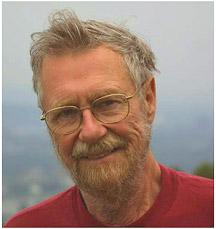
\includegraphics[width=0.25\textwidth]{figure/dijkstra.jpg}}
  \end{picture}
\end{frame}

\begin{frame}[fragile]{2.3.2 信号量机制}
  \begin{easylist} \easyitem
& 1 整型信号量
&& 是一个整型量,通过2个{\color{red}原子操作}wait(s)和signal(s)来访问。
&& Wait(s):
\begin{lstlisting}[tabsize=8,keywordstyle=\color{red},basicstyle=\small, language=Pascal, numbers=none]
while s<= 0 do no-op;
s:=s-1;
\end{lstlisting}
&& Signal(s):
\begin{lstlisting}[tabsize=8,keywordstyle=\color{red},basicstyle=\small, language=Pascal, numbers=none]
s:=s+1;
\end{lstlisting}
  \end{easylist}
\end{frame}



\begin{frame}[fragile]{2 记录型信号量}
\begin{columns}[onlytextwidth,T]
    \begin{column}{0.6 \textwidth}
\begin{lstlisting}[tabsize=8,keywordstyle=\color{red},basicstyle=\small, language=Pascal]
type  semaphore=record
        value:integer;
        L: list of process;
end
procedure wait(s)
  var s: semaphore
  begin
        s.value:=s.value - 1;
        if s.value < 0 then block (s, L)
  end
procedure signal (s)
  var s:semaphone
  begin
        s.value:=s.vaule + 1
        if s.value<=0 then wakeup(s.L)
  end
\end{lstlisting}
\end{column}
\begin{column}{0.4\textwidth}
  \small
  \begin{itemize}
  \item L:为进程链表,用于链接所有等待该类资源进程。
  \item 用wait(s)和signal(s)实现同步与互斥。
  \item 在记录型信号量机制中:
  \item s.value初值:表示系统中某类资源的数目。
  \item s.value<0:表该信号量链表中已阻塞进程的数目。
  \item Qestion: 为什么叫“记录型”信号量?
  \end{itemize}
\end{column}
\end{columns}

\end{frame}


\begin{frame}[fragile]{PV操作}
  \begin{easylist} \easyitem
    & Wait(s): 也用$P(s)$或者$Down(s)$ 表示,相当于申请资源
    & Signal(s): 也用$V(s)$ 或者$Up(s)$ 表示,相当于释放资源
    & 例如:
    && 在公共电话厅打电话
  \end{easylist}
\end{frame}


\begin{frame}[fragile]{3 AND型信号量}
  \begin{easylist} \easyitem
    & 当不用它时,有可能发生系统死锁。
    & 死锁:在无外力作用下的一种僵持状态。
    & 特点:要么全分配,要么一个也不分配。
  \end{easylist}
\end{frame}


\begin{frame}[fragile]{3 AND型信号量}
  \centering
  \begin{tabular}{| l | l |}
    \hline
    process A: & process B: \\
    wait(Dmutex); & wait(Emutex); \\
    wait(Emutex);~~~~~~ & wait(Dmutex);~~~~~~~ \\
    \hline
  \end{tabular}

  \vspace{2cm}
  若两个进程交替执行,则死锁
\end{frame}



\begin{frame}[fragile]{3 AND型信号量}
\begin{lstlisting}[tabsize=8,keywordstyle=\color{red},basicstyle=\small, language=Pascal]
Swait(s1,s2,…,sn)
    if s1 >= 1 and … and sn >= 1 then
        for i:=1 to n do si:=si-1; endfor
    else
        place the process in the waiting queue with the first si found    with si<1, and set the program count of this process to the beginning of swait operation
    end if

Ssignal(s1,s2,…,sn)
    for i:=1 to n do si:=si+1;

    remove all the process waiting in the queue associated with si into the ready queue
 endfor
\end{lstlisting}
\end{frame}

\begin{frame}[fragile]{4 信号量集}
  \begin{easylist} \easyitem
    & 某进程需要100个临界资源X时:
    && wait(x);
    && ……
    && wait(x)
    & 有些情况下,只有系统空闲资源数量大于等于一定数值,才予以分配。
  \end{easylist}
\end{frame}


\begin{frame}[fragile]{4 信号量集}
  \begin{easylist} \easyitem
    & 为提高效率而对AND信号的扩充。
    && Swait(S, t, d): t为下限制,d为需求值
    & 三种特例:
    && (1)Swait(S,d,d):允许每次申请d个资源。
    &&& 当资源数少于d时,不予分配。
    && (2)Swait (S,1,1):$S>1$,记录型信号量。
    &&& S=1时,互斥型信号量。
    && (3)Swait(S,1,0),可控开关,当$S \geq 1$时,允许进入,$S<1$时,不能进入。
  \end{easylist}
\end{frame}


\begin{frame}[fragile]{利用信号量实现互斥}
\begin{columns}[onlytextwidth,T]
\begin{column}{0.46 \textwidth}
\begin{lstlisting}[tabsize=8,keywordstyle=\color{red},basicstyle=\small, language=Pascal]
var mutex: semaphore:=1

parbegin
    process1:begin
        repeat
           wait(mutex);
           critical setion
           signal(mutex);
           remainder section
        until false;
    end
\end{lstlisting}
\end{column}
\begin{column}{0.46 \textwidth}
\begin{lstlisting}[tabsize=8,keywordstyle=\color{red},basicstyle=\small, language=Pascal, firstnumber=last]
    process2: begin
        repeat
           wait(mutex);
           critical setion
           signal(mutex);
           remainder section
        until false;
    end
parend
\end{lstlisting}
\end{column}
\end{columns}
\end{frame}


\subsection{2.4 经典进程同步问题}
\begin{frame}[fragile]{2.4 经典进程同步问题}
  \begin{easylist} \easyitem
    && 2.4.1 生产者—消费者问题
    && 2.4.2 哲学家进餐问题
    && 2.4.3 读者—写者问题
  \end{easylist}
\end{frame}

\begin{frame}[fragile]{生产者—消费者问题}
  \centering
  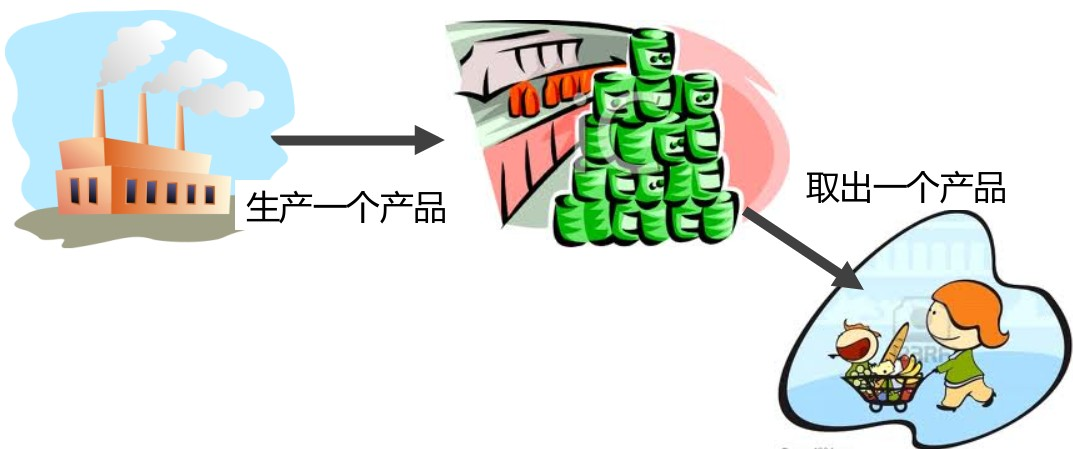
\includegraphics[width=0.85\textwidth]{figure/producer_consumer.jpg}
\end{frame}


\begin{frame}[fragile]{生产者—消费者问题}
  \begin{easylist} \easyitem
   & 定义两个同步信号量:
   && empty---表示缓冲区中空缓冲区的数量,初值为n(n个缓冲区)。
   && full---表示缓冲区中满的数量,初值为0。
   && mutex---使诸进程互斥地访问缓冲区
  \end{easylist}
\end{frame}


\begin{frame}[fragile]{记录型信号量解决生产者—消费者问题}
 \begin{lstlisting}[tabsize=8,keywordstyle=\color{red},basicstyle=\small, language=Pascal]
   var mutex,empty,full:Semaphore:=1,n,0;
       buffer:array[0,1,…,n-1] of item;
       in, out: integer: =0,0;
\end{lstlisting}
 
 \begin{columns}[onlytextwidth,T]
 \begin{column}{0.46 \textwidth}
 \begin{lstlisting}[tabsize=8,keywordstyle=\color{red},basicstyle=\small, language=Pascal, firstnumber=last, escapechar=|]
 producer: begin
     repeat
         …
         Produce an item in nextp;
         wait(empty);
         wait(mutex);
         buffer(in):=nextp;
         in:=(in+1) mod n;
         signal(mutex);
         signal(full);
     until false;
 end
 \end{lstlisting}
 \end{column} 
 \begin{column}{0.46 \textwidth}
 \begin{lstlisting}[tabsize=8,keywordstyle=\color{red},basicstyle=\small, language=Pascal, firstnumber=last, escapechar=|]
 consumer:begin
     repeat
         wait(full);
         wait(mutex);
         nextc:=buffer(out);
         out:=(out+1) mod n;
         signal(mutex);
         signal(empty);
         Consumer the item in nextc;
     until false;
 end
 \end{lstlisting}
 \end{column}
 \end{columns}
\end{frame}


 \begin{frame}[fragile]{利用AND信号量解决生产者—消费者问题}
 \begin{lstlisting}[tabsize=8,keywordstyle=\color{red},basicstyle=\small, language=Pascal]
 var  mutex, empty, full: semaphore:=1,n,0;
      buffer:array[0,…,n-1] of item;
      in out: integer :=0,0;
 \end{lstlisting}

 \begin{columns}[onlytextwidth,T]
 \begin{column}{0.46 \textwidth}
 \begin{lstlisting}[tabsize=8,keywordstyle=\color{red},basicstyle=\small, language=Pascal, firstnumber=last]
 producer: begin
     repeat
         …
         Produce an item in nextp;
         Swait(empty, mutex);
         buffer(in):=nextp;
         in:=(in+1) mod n;
         Ssingal(mutex, full);
     until false;
 end
 \end{lstlisting}
 \end{column}
 \begin{column}{0.46 \textwidth}
 \begin{lstlisting}[tabsize=8,keywordstyle=\color{red},basicstyle=\small, language=Pascal, firstnumber=last]
 consumer:begin
     repeat
         Swait(full, mutex);
         nextc:=buffer(out);
         out:=(out+1) mod n;
         Ssignal(mutex, empty);
         consumer the item in nextc;
     until false;
 end
 \end{lstlisting}
 \end{column}
 \end{columns}
\end{frame}



\begin{frame}[fragile]{2.4.2 哲学家进餐问题}
  \begin{columns}[onlytextwidth,T]
    \column{0.46 \textwidth}
    \par 有五个哲学家围坐在一圆桌旁,桌中央有一盘通心面,每人面前有一只空盘子,每两人之间放一把叉子。每个哲学家思考、饥饿、然后吃通心面。为了吃面,每个哲学家必须获得两把叉子,且每人只能直接从自己左边或右边去取叉子。

    \column{0.46 \textwidth}
    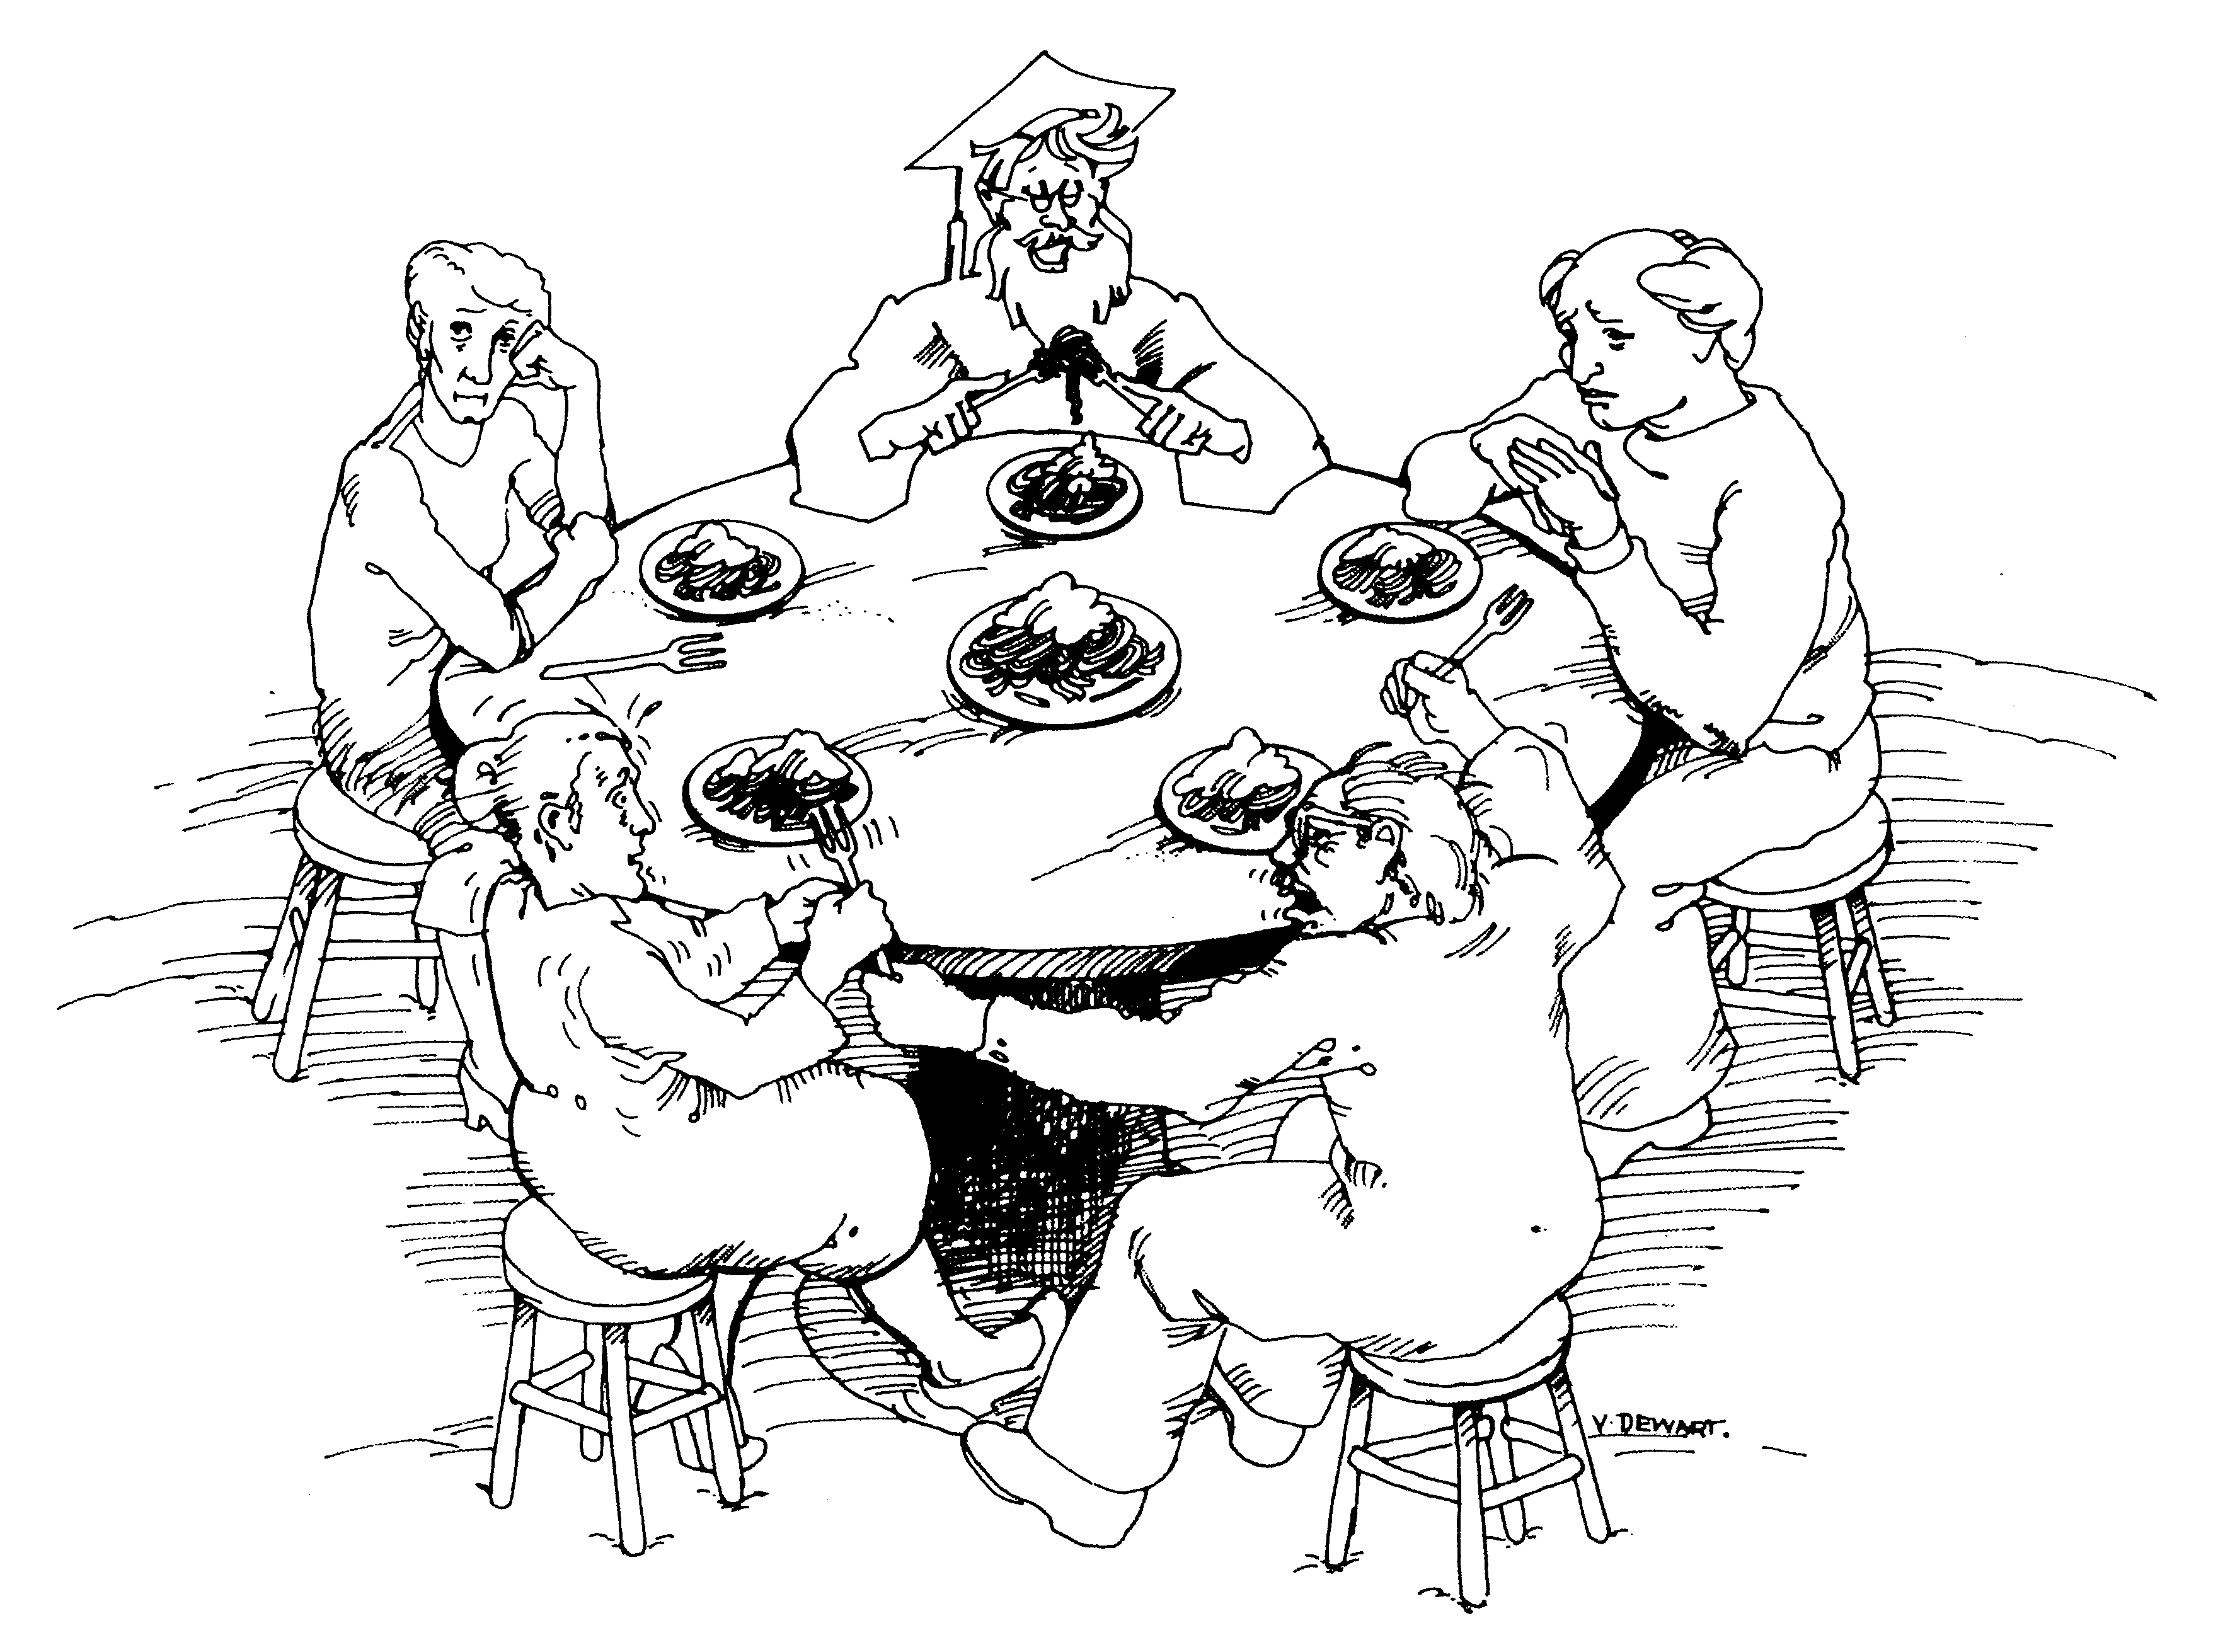
\includegraphics[width=1.0\textwidth]{figure/dining.jpg}
  \end{columns}
\end{frame}

\begin{frame}[fragile]{哲学家进餐问题解决思路}
  \begin{easylist} \easyitem
    & 1、每一把叉子都是必须互斥使用的,所以,必须为每一把叉子设置一个互斥信号量
    $S_i$ ($i = 0,1,2,3,4$);
    & 2、初值都为1;
    & 3、当一个哲学家吃面时必须获得自己左边和右边的两把叉子,即执行两个$P$操作($wait$);吃完面后,必须放下两个叉子,即执行两个$V$操作($signal$)。
  \end{easylist}
\end{frame}

\begin{frame}[fragile]{利用记录型信号量解决哲学家进餐问题}
第i个哲学家:

\begin{lstlisting}[tabsize=8,keywordstyle=\color{red},basicstyle=\small, language=Pascal]
var chopstick: array[0, …, 4] of semaphore;
repeat
    wait(chopstick[i]);
    wait(chopstick[(i+1)mod 5]);
    …
   eat
    …
   signal(chopstick[i]);
   signal(chopstick[(i+1)mod 5]);
    …
   think;
until false
\end{lstlisting}
\end{frame}

\begin{frame}[fragile]{利用AND信号量解决哲学家进餐问题}
\begin{lstlisting}[tabsize=8,keywordstyle=\color{red},basicstyle=\small, language=Pascal]
var chopstick: array[0, …, 4] of semaphore:=(1,1,1,1,1);
processi
    repeat
       think;
       Sswait(chopstick[(i+1) mod 5],chopstick[i]);
       eat
       Ssignal(chopstick[(i+1) mod 5],chopstick[i]);
    until false
\end{lstlisting}
\end{frame}

\begin{frame}[fragile]{课堂练习}
  \large
  \begin{easylist} \easyitem
    & 请利用记录型信号量写出一个不会死锁的哲学家进餐问题的算法。
  \end{easylist}
\end{frame}

\begin{frame}[fragile]{2.4.3 读者—写者问题}
  \large
  \begin{easylist} \easyitem
    & 读者写者问题
    && 有两组并发进程:
    &&& 读者和写者,共享一组数据区
    && 要求:
    &&&  允许多个读者同时执行读操作
    &&& 不允许读者、写者同时操作
    &&&  不允许多个写者同时操作
    & 特点:
    && 读进程可共享同一对象。
    && 写进程不可共享同一对象。
  \end{easylist}
\end{frame}



\begin{frame}[fragile]{利用记录型信号量解决读者—写者问题 I}
\begin{lstlisting}[tabsize=8,keywordstyle=\color{red},basicstyle=\small, language=Pascal, escapechar=|]
var rmutex, wmutex: semaphore: =1,1;
    readcount:integer: =0;
begin
    parbegin
\end{lstlisting}
\end{frame}

\begin{frame}[fragile]{利用记录型信号量解决读者—写者问题 II}
\begin{lstlisting}[tabsize=8,keywordstyle=\color{red},basicstyle=\small, language=Pascal,firstnumber=last, escapechar=|]
      reader: begin
        repeat
            wait(rmutex);
            if readcount=0 then wait(wmutex);
            readcount:=readcount+1;
            signal(rmutex);

            ...
            perform read operation
            ...

            wait(rmutex);
            readcount:=readcount-1;
            if readcount=0 then signal(wmutex);
            signal(rmutex);
       until false;
     end
\end{lstlisting}

% \begin{tikzpicture}[overlay, remember picture]
%   \draw node[draw, below right=of rwquestion, ellipse] (tip) { 读者如何被唤醒?};
%   \path[draw=orange,->] (rwquestion) edge [bend right=15] (tip);
% \end{tikzpicture}

\end{frame}

\begin{frame}[fragile]{利用记录型信号量解决读者—写者问题 III}
\begin{lstlisting}[tabsize=8,keywordstyle=\color{red},basicstyle=\small, language=Pascal,firstnumber=last, escapechar=|]
     writer: begin
       repeat
           wait(wmutex)
           perform write operation;
           signal(wmutex)
        until false;
      end
    parend
end
\end{lstlisting}
\end{frame}


\begin{frame}[fragile, allowframebreaks]{信号量集解决读者—写者问题(略)}
\begin{lstlisting}[tabsize=8,keywordstyle=\color{red},basicstyle=\small, language=Pascal]
var RN integer;
        L, mx: semaphore: =RN, 1;
 begin
   parbegin
     reader: begin
        repeat
               swait(L,1,1);
               swait(mx,1,0);
                 …
               perform read operation;
                 …
               ssignal(L,1);
         until false;
      end
      writer: begin
         repeat
               swait(mx,1,1; L,RN,0);
               perform write operation;
               ssignal(mx, 1);
         until flase;
      end
    parend
  end
\end{lstlisting}
\end{frame}

\begin{frame}[fragile]{上述方法为读者优先}
  \begin{easylist} \easyitem
    & 如果读者来:
    && (1) 无读者、写者,新读者可以读
    && (2) 有写者等,但有其它读者正在读,则新读者也可以读
    && (3) 有写者写,新读者等
    & 如果写者来:
    && (1) 无读者,新写者可以写
    && (2) 有读者,新写者等待
    && (3) 有其它写者,新写者等待
  \end{easylist}
\end{frame}





\begin{frame}[fragile]{读者优先分析}
  \begin{easylist} \easyitem
    & 问题:
    && 读者源源不断,readCount不归0,写者会被饿死。
    & 策略:
    && 一旦有写者等待,新到达读者等待,正在读的读者都结束后,写者进入。
  \end{easylist}
\end{frame}

\begin{frame}[fragile]{写者优先}
  \begin{easylist} \easyitem
    & 条件:
    && (1) 多个读者可以同时进行读
    && (2) 写者必须互斥(只允许一个写者写,也不能读者写者同时进行)
    && (3) 写者优先于读者(一旦有写者,则后续读者必须等待,唤醒时优先考虑写者)
    \vspace{2cm}
    & 练习尝试
  \end{easylist}
\end{frame}


\begin{frame}[fragile, allowframebreaks]{写者优先(采用类Java/C伪代码)}
\begin{lstlisting}[tabsize=8,keywordstyle=\color{red},basicstyle=\small, language=c]
Semaphore fmutex=1, rdcntmutex=1, wtcntmutex=1, queue=1;
//fmutex: access to file;
// rdcntmutex: access to readcount
//wtcntmutex: access to writecount
int readcount = 0, writecount = 0;

void reader(){
    while(true){
        wait(queue);
        wait(rdcntmutex);
        if(0 == readcount)wait(fmutex);
        readcount = readcount + 1;
        signal(rdcntmutex);
        signal(queue);

        //reading ...

        wait(rdcntmutex);
        readcount = readcount - 1;
        if(0 == readcount) signal(fmutex);
        signal(rdcntmutex);
    }
}

void writer(){
    while(true){
        wait(wtcntmutex);
        if(0 == writecount)wait(queue);
        writecount = writecount + 1;
        signal(wtcntmutex);

        wait(fmutex);
        //writing ...
        signal(fmutex);

        wait(wtcntmutex);
        writecount = writecount - 1;
        if(0 == writecount)signal(queue);
        signal(wtcntmutex);
    }
}
\end{lstlisting}
\end{frame}


\begin{frame}[fragile]{练习}
  \begin{easylist} \easyitem
    & a,b 两点间是一段东西向的单行车道,现要设计一个自动管理系统,管理规则如下:
    && 当ab间有车辆在行驶时,同方向的车可以继续驶入ab段,但另一方向的车必须在ab段外等待;
    && 当ab之间无车时,到达a(或b)的车辆可以进入ab段,但不能从a,b点同时驶入;
    && 当某方向在ab段行驶的车辆使出了ab段且无车辆进入ab段时,应让另一方向等待的车辆进入ab段行驶。
    \vspace{1cm}
    & 请用wait,signal工具对ab段实现正确管理。
  \end{easylist}
\end{frame}

\begin{frame}[fragile, allowframebreaks]{练习答案}
\begin{lstlisting}[tabsize=8,keywordstyle=\color{red},basicstyle=\small, language=Pascal]
semaphore s, mutexab,mutexba
integer countab = 0, countba = 0
pab:
    wait(mutexab);
    countab++;
    If countab=1 then wait(s);
    signal(mutexab);
    …
    wait(mutexab);
    countab--;
    if countab=0 then signal(s);
    signal(mutexab);
\end{lstlisting}
\newpage
\begin{lstlisting}[tabsize=8,keywordstyle=\color{red},basicstyle=\small, language=Pascal,firstnumber=last]
pba:
    wait(mutexba);
    countba=countba+1;
    if countba=1 then wait(s);
    signal(mutexba);
    enter;
    ……
    wait(mutexba);
    countba--;
    if countba=0 then signal(s);
    signal(mutexba);
\end{lstlisting}
\end{frame}

\begin{frame}[fragile]{作业讨论}
  \begin{easylist} \easyitem
    & 无死锁的哲学家进餐问题
    & 写者优先
  \end{easylist}
\end{frame}



\begin{frame}[fragile]{练习}
  \begin{easylist} \easyitem
    & 设有两个生产者进程A、B和一个销售者进程C,他们共享一个无限大的仓库
    && 生产者每次循环生产一个产品,然后入库供销售者销售;
    && 销售者每次循环从仓库中取出一个产品进行销售。
    && 不允许同时入库,也不允许边入库边出库;
    && 要求生产和销售A产品和B产品的件数都满足以下关系:
    &&& $-n \leqslant$ A生产的件数$-$ B生产的件数$\leqslant m$,
    &&& $-n \leqslant$ A销售的件数$-$ B销售的件数$\leqslant m$,
    &&& 其中$m, n$是正整数。
    \vspace{1cm}
    & 使用信号量机制写出A、B和C三个进程的工作流程
  \end{easylist}
\end{frame}

\begin{frame}[fragile]{分析}
  \begin{easylist} \easyitem
    & 设置信号量mutext,互斥访问仓库
    & 为满足$-n \leq A$的件数$-B$的件数$\leq m$,设置两个同步信号量
    && $SAB$:允许A当前生产的数量,初值为$m$
    && $SBA$:允许B当前生产的数量,初值为$n$
    & 为实现生产者和销售者的同步,
    && 设置变量Difference:表示A与B所销售的数量之差,初值为0
    && 设置三个信号量:S、SA、SB,分别表示仓库中总的产品量、仓库中A的产品量和B的产品量,初值为0
  \end{easylist}
\end{frame}


\begin{frame}[fragile]{生产者}
  \begin{columns}[T]
    \column{0.47\textwidth}
    \begin{lstlisting}[tabsize=8,keywordstyle=\color{red},basicstyle=\small, language=Pascal]
Process A:
repeat
    wait(SAB)
    produce a product A
    signal(SBA)

    //加入仓库
    wait(mutex)
    add A to storehouse
    signal(mutex)

    siganl(SA)
    signal(S)
until false \end{lstlisting}
    \column{0.47\textwidth}
    \begin{lstlisting}[tabsize=8,keywordstyle=\color{red},basicstyle=\small, language=Pascal,firstnumber=last]
Process B
repeat
    wait(SBA)
    produce a product B
    signal(SAB)

    //加入仓库
    wait(mutex)
    add B to storehouse
    signal(mutex)

    siganl(SB)
    signal(S)
until false \end{lstlisting}
  \end{columns}
\end{frame}


\begin{frame}[fragile]{销售者C}
  \begin{columns}[T]
    \column{0.47\textwidth}
    \begin{lstlisting}[tabsize=8,keywordstyle=\color{red},basicstyle=\small, language=c]
Repeat
    wait(S)
    if (difference<=-n) { //B卖的太多了
        wait(SA)
        wait(mutex)
        take a product A
        signal(mutex)
        difference += 1
    } else if(difference >=m) { //A卖的太多了
        wait(SB)
        wait(mutex)
        take B
        signal(mutex)
        difference -= 1  \end{lstlisting}

    \column{0.47\textwidth}
    \begin{lstlisting}[tabsize=8,keywordstyle=\color{red},basicstyle=\small, language=c,firstnumber=last]
    } else{
        wait(mutex)
        take product A or B
        signal(mutex)
        if(type==A){
            wait(SA)
            difference+=1
         } else {
            wait(SB)
            difference -=1
         }
    }
    Sell product
until false  \end{lstlisting}
  \end{columns}
\end{frame}


\begin{frame}[fragile]{练习(嗜睡的理发师问题)}
  \begin{easylist} \easyitem
    & 一个理发店由一个有N张沙发的等候室和一个放有一张理发椅的理发室组成。
    & 没有顾客时,理发师便去睡觉。
    & 当一个顾客走进理发店时,如果所有的沙发都已被占用,便离开理发店;否则,如果理发师正在为其他顾客理发,该顾客就找一张空沙发坐下等待;如果理发师因无顾客正在睡觉,则由新到的顾客唤醒理发师为其理发。在理发完成时,顾客必须付费,直到理发师收费后才能离开理发店。
    \vspace{0.8cm}
    & 试用信号量实现这一同步问题
  \end{easylist}
\end{frame}

\begin{frame}[fragile]{分析}
  \begin{easylist} \easyitem
    & 设置整型变量count,记录顾客数;
    & 设置mutex信号量,保证对count的互斥,初值为1
    & 对等候室中的N张沙发,设置信号量sofa,初值为N
    & empty信号量表示是否有空闲的理发椅,初值为1
    & full表示理发椅上是否有等待理发的顾客,初值为0
    & cut信号量表示理发是否完成,初值为0
    & payment表示等待付费,初值为0
    & receipt表示等待收费,初值为0
  \end{easylist}
\end{frame}

\begin{frame}[fragile]{顾客}
  \begin{columns}[T]
    \column{0.47\textwidth}
    \begin{lstlisting}[tabsize=8,keywordstyle=\color{red},basicstyle=\scriptsize, language=c]
wait(mutex)
if(count>N){
    signal(mutex)
    exit
} else {
    count++;
    signal(mutex)
    if(count>1) {
        wait(sofa)
        sit on
        wait(empty)
        get up from sofa
        signal(sofa)
    } else {
        wait(empty)
    }
    ...
}  \end{lstlisting}
    \pause

    \column{0.47\textwidth}
    \begin{lstlisting}[tabsize=8,keywordstyle=\color{red},basicstyle=\small, language=c,firstnumber=last]
sit on baber_chair
signal(full)
wait(cut)
pay
signal(payment)
wait(receipt)
get up from baber_chair
signal(empty)
wait(mutex)
count--
siganl(mutex)
exit shop  \end{lstlisting}
  \end{columns}
\end{frame}




\begin{frame}[fragile]{理发师}
 \begin{lstlisting}[tabsize=8,keywordstyle=\color{red},basicstyle=\small, language=c]
while(true){
    wait(full)
    cut hair
    signal(cut)
    wait(payment)
    accept payment
    signal(recipt)
} \end{lstlisting}
\end{frame}


\subsection{2.5 管程机制}
\begin{frame}[fragile]{2.5 管程机制}
  \begin{easylist} \easyitem
    & 70年代初, By
    && E.W.Dijkstra, C.A.R.Hoare, P.B.Hansen.
    && 背景:  Structured programming
    & 引入原因:
    && 为了避免凡要使用临界资源的进程都自备同步操作wait(s)和signal(s).将同步操作
    的机制和临界资源结合到一起,形成管程。
    && 信号量程序编写困难
    && 让困于人:将信号量的组织工作交给一个专门的机构负责,解脱程序员。
  \end{easylist}
\end{frame}

\begin{frame}[fragile]{2.5.1 管程的基本概念}
  \begin{easylist} \easyitem
    & 一、定义:一个数据结构和能为并发进程所执行的一组操作。
    && 局部于管程的共享变量。
    && 对该数据结构进程操作的一组过程。
    && 对局部管程数据设置初值。
    & 二、条件变量:
    && x.y:  x.wait; x.signal;  x.queue
  \end{easylist}
\end{frame}

\begin{frame}[fragile, allowframebreaks]{2.5.2 利用管程解决生产者—消费者问题}
  \begin{easylist} \easyitem
    & 一、建立管程:PC
    && 包括:二过程:		
    &&& (1)put(item)过程;
    &&& (2)get(item)过程
    && 一变量:$count \geqslant n$时满;$\leqslant 0$时空
    && 初始:  in=out=count=0
  \end{easylist}
\begin{lstlisting}[tabsize=8,keywordstyle=\color{red},basicstyle=\small, language=Pascal]
type producer-consumer=monitor
    var in,out,count:integer;
    buffer: array [0,…,n-1] of item;
    notfull, notempty: condition;
    procedure entry put (item)
    procedure entry get (item)
\end{lstlisting}

\newpage
\begin{lstlisting}[tabsize=8,keywordstyle=\color{red},basicstyle=\small,
  language=Pascal, firstnumber=last]
Procedure entry put(item)
	begin
	  if count >= n then notfull.wait;
	    buffer(in):=nextp;
	    in:=(in+1)mod n
	    count:=count+1;
	    if notempty.queue then notempty.signal;
	end
Procedure entry get(item)
	begin
	  if count <= 0 then notempty.wait;
	    nextc:=buffer(out);
	    out:=(out+1)mod n
	    count:=count-1;
	    if notfull.queue then notfull.signal;
	end
Begin in:=out:=0;   count:=0 end

producer: begin
    repeat
        produce an item in nextp
        PC. put (item);
    until false.
end
consumer: begin
    repeat
        PC.get(item);
        consume the item in nextc;			
    until false
end 
\end{lstlisting}
\end{frame}

\begin{frame}[fragile]{PV操作与管程对比}
  \begin{columns}[T]
    \column{0.48\textwidth}
      PV操作: 

      ~~(1) 分散式同步机制:共享变量操作,PV操作,分散在整个系统中或各个
      进程中。 \\
      ~~(2) 缺点:\\
      ~~~~(a)可读性差;\\
      ~~~~(b)正确性不易保证;\\
      ~~~~(c)不易修改。 \\
      ~~(3) 优点:高效,灵活。
    
    \column{0.48\textwidth}
     管程:

      ~~(1) 集中式同步工具:共享变量及其所有相关操作集中在一个摸块中。\\
      ~~(2) 优点:\\
      ~~~~(a)可读性好;\\
      ~~~~(b) 正确性易于保证;\\
      ~~~~(c) 易于修改。\\
      ~~(3) 缺点:不甚灵活,效率略低。
    \end{columns}
\end{frame}

\subsection{2.6 进程通信}
\begin{frame}[fragile]{2.6 进程通信}
  \begin{easylist} \easyitem
    & 概念:进程间的信息交换。
    & 实例:
    && 信号量机制(一种低级通信)
    &&& 缺点:
    &&&& (1)效率低
    &&&& (2)通信对用户不透明
    && 高级通信特点:
    &&& 效率高,通信实现细节对用户透明
  \end{easylist}
\end{frame}

\begin{frame}[fragile, allowframebreaks]{2.6.1 进程通信的类型}
  \begin{easylist} \easyitem
    & 一、共享存贮器系统
    && 1.基于共享数据结构的通信方式:
    &&& produce-consume中的缓冲区,低效,不透明。
    &&& 系统只提供了一共享存贮器,适于少量通信。
    && 2.基于共享存储区的通信方式:
    &&& 系统提供:共享存储区。
    &&& 通信过程:
    &&&& (1)向系统申请一个或多个分区
    &&&& (2)获得分区获后即可读/写.
    &&& 特点:高效,速度快。
    \newpage
    \vspace{0.5cm}
    & 二、消息传递系统(可用于异种机)
    && 信息单位:消息(报文)
    && 是目前的主要通信方式,分为直接通信方式、间接通信方式
    && 实现:一组通信命令(原语),具有透明性 同步的实现。

    & 三、管道通信
    && 管道:连接一个读进程和一个写进程之间通信的共享文件。
    && 功能:大量的数据发收。
    && 注意:
    &&& (1)互斥
    &&& (2)同步
    &&& (3)对方是否存在
  \end{easylist}
\end{frame}

\begin{frame}[fragile, allowframebreaks]{2.6.2 消息传递通信的实现方法}
  \begin{easylist} \easyitem
    & 一、直接传递方式
    && send(Receiver, message)
    && receive(Sender, message)
    && 例:解决生产—消费问题
  \end{easylist}
\begin{lstlisting}[tabsize=8,keywordstyle=\color{red},basicstyle=\small, language=Pascal]
  repeat
       produce an item in nextp;
       ...
       send(consumer, nextp);
  until false;
  repeat
         receive( producer, nextc);
         ...
         consumer the item in nextc;
   until false;
\end{lstlisting}

\newpage
  \vspace{1cm}
  \begin{easylist} \easyitem
    & 二、间接(可以实现非实时通信)
    && 优点:在读/写时间上的随机性
    && 写进程 $\rightarrow$ 信箱(中间实体)$\rightarrow$ 读进程
    && 原语
    &&& (1)信箱的创建与撤消:
    &&&& 信箱名  属性(公用、私用、共享)(共享者名字)
    &&& (2)消息的发送和接收
    &&&& Send (mailbox, message)
    &&&& Receive (mailbox, message)
\newpage
\vspace{1cm}
    && 信箱类型
    &&& (1)私用:拥有者有读/写数,其它只有写权,(单向)存在期=进程存在期。
    &&& (2)公用:系统创建, 双向, 存在期=系统存在期。
    &&& (3)共享信箱:一般进程创建,并指明其共享者,是双向。
    && 发送—接收进程之间的关系:
    &&& (1)一对一关系;
    &&& (2)多对一关系;(客户-服务器方式)
    &&& (3)一对多关系;(适用于广播方式)
    &&& (4)多对多关系:公用信箱
  \end{easylist}
\end{frame}


\begin{frame}[fragile, allowframebreaks]{2.6.3 消息传递系统中的几个问题}
  \begin{easylist} \easyitem
    & 一、通信链路:
    && (1)显式建立:(进程完成、网络中)
    && (2)隐式建立:(系统完成、单机中)
    && 链路类型:
    &&& (1)由连接方法分:点—点链路,多点链路。
    &&& (2)由通信方式分:单向、双向。
    &&& (3)由容量分:无容量(无缓冲区)、有(有缓冲区)。
    \newpage
    & 二、消息格式:
    && 格式组成
    &&& 消息头:含控制信息如:收/发进程名,消息长度、类型、编号
    &&& 消息内容:
    && 格式类型
    &&& 定长消息:系统开销小,用户不便(特别是传长消息用户)
    &&& 变长消息:开销大,用户方便。
    \newpage
    & 三、进程同步方式
    && 1.发送和接收进程阻塞(汇合)
    &&& 用于紧密同步,无缓冲区时。
    && 2.发送进程不阻塞,接收进程阻塞(多个)
    &&& 相当于接收进程(可能是多个)一直等待发送进程,如:打印进程等待打印任务。
    && 3.发送/接收进程均不阻塞
    &&& 一般在发、收进程间有多个缓冲区时。
  \end{easylist}
\end{frame}


\subsection{2.7 线程}
\begin{frame}[fragile]{2.7 线程}

  \begin{easylist} \easyitem
    & Single and Multithreaded Processes    
  \end{easylist}

  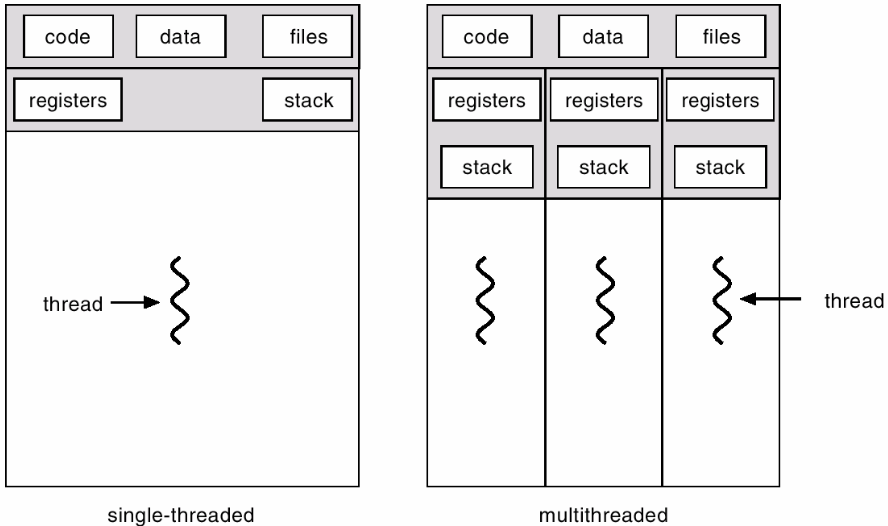
\includegraphics[width=0.9\textwidth]{figure/thread_single_vs_multi.png}
\end{frame}


\begin{frame}[fragile]
  \frametitle{2.7.1 线程的的基本概念(1)}
  1. 线程的优势:
  \begin{easylist} \easyitem
    & 响应速度(Responsiveness)
    && 减少并发执行时的时空开销,进程的创建、撤消、切换较费时空,因它既是调度单位,又是资源拥有者。

    & 资源共享(Resource Sharing)
    && 线程是系统独立调度和分派的基本单位,其基本上不拥有系统资源,只有少量资源
    (寄存器,栈…),但共享其所属进程所拥有的全部资源。
    
    & 充分利用多核/多处理器的硬件性能
    (Utilization of MP \& Multicore Architectures)
  \end{easylist}
\end{frame}


\begin{frame}[fragile]{2.7.1 线程的基本概念(2)}
  \begin{easylist} \easyitem
    & 2.线程的属性
    && 轻型实体
    && 独立调度和分派的基本单位
    && 可并发实体
    && 共享进程资源
    & 3.线程的状态
    && 状态参数
    &&& 寄存器状态、堆栈、运行状态、优先级、线程专有存储器、
    &&& 信号屏蔽
    && 线程的运行状态 
    &&& 就绪、执行、阻塞
  \end{easylist}
\end{frame}

\begin{frame}[fragile]{2.7.1 线程的基本概念(3)}
  \begin{easylist} \easyitem
    & 4.线程的创建和终止
    && 初始化线程
    & 5.多线程中的进程
    && 进程是拥有系统资源的基本单位,但不再是一个可执行的实体。
  \end{easylist}
\end{frame}

\begin{frame}[fragile]
  \frametitle{2.7.2 线程的类型}
  \begin{easylist}
  & 用户线程(User-level thread)
  && Thread management done by user-level threads library

  && 三种常见的用户线程
  &&& POSIX Pthreads
  &&& Win32 threads
  &&& Java threads
  
  & 内核线程(Kernel-Level Thread)
  && Supported by the Kernel
  &&& Windows XP/2000 ...
  &&& Linux
  &&& Mac OS X
  \end{easylist}
\end{frame}

\begin{frame}[fragile]
  \frametitle{用户线程向内核线程的映射}
  目的:把用户线程转换为内核线程,从而由操作系统调度执行
  \begin{easylist}
    & Many to One
    && Solaris Green Threads
    && GNU Portable Threads

    & One to One
    && Windows
    && Linux
    && Solaris 9 and later
    
    & Many to Many
    && Solaris prior to version 9
    && Windows NT/2000 with the ThreadFiber package
  \end{easylist}
\end{frame}

\begin{frame}[fragile]
  \frametitle{Many-to-one Model}
  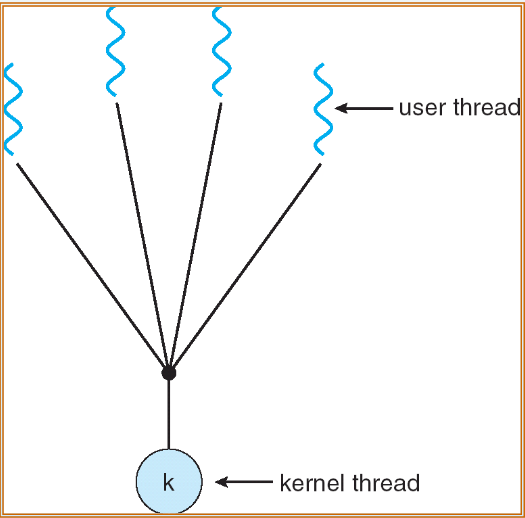
\includegraphics[width=0.6\textwidth]{figure/thread_many2one.png}
\end{frame}


\begin{frame}[fragile]
  \frametitle{One-to-one Model}
  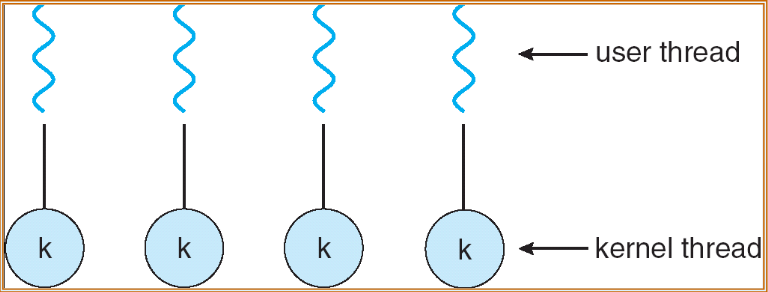
\includegraphics[width=0.9\textwidth]{figure/thread_one2one.png}
\end{frame}


\begin{frame}[fragile]
  \frametitle{Many-to-Many Model}
  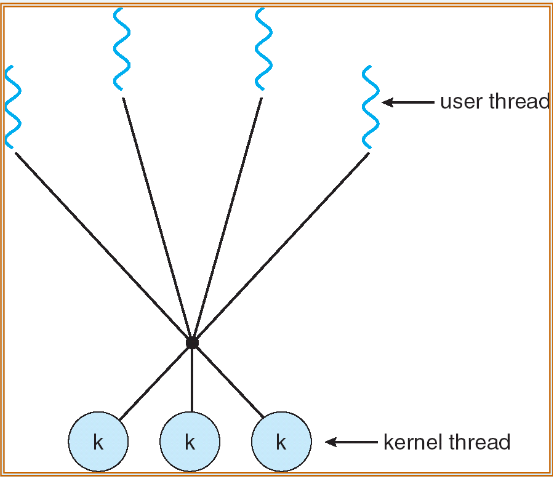
\includegraphics[width=0.6\textwidth]{figure/thread_many2many.png}
\end{frame}

\begin{frame}[fragile]{2.7.3 线程的同步和通信}
  \begin{easylist} \easyitem
    & 1.互斥锁
    && 阻塞方式 \\
    lock(mutex)\\
    访问\\
    unlock(mutex)\\

    && 非阻塞方式 \\
    if(trylock) then \\
    else \\
  \end{easylist}
\end{frame}

\begin{frame}[fragile]{2.7.3 线程的同步和通信}
  \begin{easylist} \easyitem
    & 2.条件变量
    && 用于线程的长期等待
    & 3.信号量机制
    && 私用信号量(private semaphore)
    &&& 作用域在一个进程中
    && 公用信号量(public semaphore)
    &&& 作用于多个进程间
  \end{easylist}
\end{frame}

\begin{frame}[fragile, allowframebreaks]{练习}
  \begin{enumerate}
  \item 进程的并发执行是指若干个进程( {\color{white} B}  ) \\
    A、同时执行          \\
    B、在执行的时间上是重叠的\\
    C、在执行的时间上是不可重叠的\\  
    D、共享系统资源 \\

  \item 若PV操作的信号量S初值为2,当前值为-1,则表示有( {\color{white} B}  )个等待进程。\\
    A、0个 \hspace{1cm}    B、1个 \hspace{1cm}   C、2个  \hspace{1cm}    D、3个

  \item 用PV操作管理临界区时,信号量的初值应定义为( {\color{white} C}  ) \\
    A、-1  \hspace{1cm}    B、0  \hspace{1cm}    C、1   \hspace{1cm}   D、任意值

  \item 用V操作唤醒一个等待进程时,被唤醒进程的状态变为( {\color{white} B}  ) \\
    A、等待  \hspace{1cm}  B、就绪   \hspace{1cm}  C、运行  \hspace{1cm}  D、完成

  \item ( {\color{white} D} )是一种只能进行P操作和V操作的特殊变量。(PV操作只能在
    ( {\color{white} D} )上操作) \\
    A、调度  \hspace{1cm} B、进程  \hspace{1cm} C、同步  \hspace{1cm} D、信号量

  \item 对于两个并发进程,设互斥信号量为mutex,若mutex=0,则({\color{white} B} ) \\
    A、表示没有进程进入临界区 \\
    B、表示有一个进程进入临界区 \\
    C、表示有一个进程进入临界区,另一个进程等待进入 \\
    D、表示有两个进程进入临界区 \\

  \item 临界区是({\color{white} C} ) \\
    A、一个缓冲区  \hspace{1cm} B、一段共享数据区  \\
    C、一段程序代码 \hspace{1cm}  D、一个互斥资源

  \item 信号量的物理意义是当信号量大于零时表示({\color{white} 可用资源数目} );
    当信号量小于零时,其绝对值为({\color{white} 因请求该资源而被阻塞的进程数目} )。

  \item 临界资源的概念是({\color{white} 一次仅允许一个进程访问的资源} ),而临界
    区是指({\color{white} 进程中访问临界资源的那段程序代码} )。

  \item 若一个进程已进入临界区,其它欲进入临界区的进程必须({\color{white} 等待} )。

  \item 用PV操作管理临界区时,任何一个进程在进入临界区之前应调用({\color{white}
      P} )操作,退出临界区时应调用({\color{white} V} )操作。

  \item 有m个进程共享同一临界资源,若使用信号量机制实现对临界资源的互斥访问,则信
    号量的变化范围是({\color{white} [-(m-1),1]} )。

  \item 操作系统中,对信号量S的P原语的定义中,使进程进入相应等待队列等待的条件是({\color{white} S<0} )。

  \item 如果信号量的当前值为-4,则表示系统中在该信号量上有({\color{white} 4} )个等待进程。

  \item 并发进程之间的基本关系是({\color{white} 互斥} )或({\color{white} 同步} )。
    其中({\color{white} 互斥} )是指进程之间的一种间接的关系。

  \end{enumerate}
\end{frame}



\begin{frame}[fragile]{本章作业及延伸阅读}
  \begin{easylist} \easyitem
    & 作业:操作系统同步之信号量机制

    根据文章介绍,实现并进行体验。https://zhuanlan.zhihu.com/p/34410587

    要求:以Markdown格式交作业,包括但不限于以下部分:

    && 整个测试流程及代码
    && 心得体会
    && 个人信息

    & 阅读(不用交):关于现代CPU,程序员应当更新的知识:

    http://www.iteye.com/news/30978
  \end{easylist}
\end{frame}



\begin{frame}[fragile]{}
 ~ 
\begin{center}
  --- END ---
\end{center}

\end{frame}

\section{处理机的调度与死锁}

\begin{frame}[fragile]{CH3 处理机的调度与死锁}
  \begin{easylist} \easyitem
    & 3.1 处理机调度的基本概念
    & 3.2 调度算法
    & 3.3 实时调度
    & 3.4 多处理机系统中的调度
    & 3.5 产生死锁的原因和必要条件
    & 3.6 预防死锁的办法
    & 3.7 死锁的检测与解除
  \end{easylist}
\end{frame}

\begin{frame}[fragile]
  \frametitle{进程一章的补充阅读作业}
  协程介绍:介绍协程的历史,现在和未来,协程与进程、线程的差异等

  所有人整理的文档下周一前发助教。
    
  下周开始小组汇报(学习委员按照人数分成10个小组)

\end{frame}


\subsection{3.1 处理机调度的基本概念}
\begin{frame}[fragile]{3.1 处理机调度的基本概念}
  \begin{easylist} 
    & 进程调度的定义和目标
    & 高级、中级和低级调度
    & 调度队列模型
    & 选择调度方式和调度算法的若干准则
  \end{easylist}
\end{frame}

\begin{frame}[fragile]{进程调度的定义}
  \begin{easylist} \easyitem
    & 单CPU环境下,任一时刻只能有一个进程处于执行状态,如何确定在某一时刻由哪个
    进程执行?
    & 调度:
    && 根据特定目标选择下一个要运行的进程
    && 调度的级别或者说粒度问题?
  \end{easylist}
\end{frame}

\begin{frame}[fragile]{高级、中级和低级调度}
  \begin{easylist} \easyitem
    & 高级调度
    && 作业调度、长程调度、接纳调度
    & 中级调度
    & 低级调度
    && 进程调度,短程调度
    \vspace{1cm}
    & 运行频率:低 $\backsim$ 中 $\backsim$ 高
  \end{easylist}
\end{frame}


\begin{frame}[fragile]{高级调度}
  \begin{easylist} \easyitem
    & 确定将哪些外存作业调入内存之中,进而创建PCB等,插入就绪队列
    & 一般用于批处理系统,分/实时系统一般直接入内存,无此环节
    \vspace{1cm}
    & 调度特性
    && 1.接纳作业数(内存驻留数)
    &&& 太多 $\Rightarrow$  周转时间T长
    &&& 太少 $\Rightarrow$  系统效率低
    && 2.接纳策略:
    &&& 即采用何种调度算法:FCFS、短作业优先、基于作业优先权的调度、响应比高者优先等
  \end{easylist}
\end{frame}


\begin{frame}[fragile]{低级调度}
  \begin{easylist}
    & 主要是由分派程序(Dispatcher)分派处理机。
    & 1.非抢占方式:
    && 简单,实时性差  (如win31)
    & 2.抢占方式
    && (1)时间片原则
    && (2)优先权原则
    && (3)短作业优先原则。   
  \end{easylist}
\end{frame}


\begin{frame}[fragile]{中级调度}
  \begin{easylist} \easyitem
    & 为提高系统吞吐量和内存利用率而引入的内外存对换功能(换出时,进程为挂起或就绪驻外状态) 
    & 典型代表:存储器管理中的对换功能
  \end{easylist}
\end{frame}


\begin{frame}[fragile, allowframebreaks]{选择调度方式和算法的准则}
  \begin{easylist} \easyitem
    & 一、面向用户的准则: 周转时间、响应时间
    && 1.周转时间短(常用于批处理系统)
    &&& 概念:作业从提交到完成的时间,分为:
    &&&& (1)驻外等待调度时间
    &&&& (2)驻内等待调度时间
    &&&& (3)执行时间
    &&&& (4)阻塞时间
    && 2.响应时间快:(对交互型作业)
    &&& 概念:键盘提交请求到首次响应时间
    &&&& (1)输入传送时间
    &&&& (2)处理时间
    &&&& (3)响应传送时间
    && 3.截止时间的保证(特别于实时系统)
    && 4.优先权准则:(即需要抢占调度)

    & 二、面向系统的准则
    && 1.吞吐量高(特别于批处理):单位时间完成作业数
    && 2.处理机利用率好:(因CPU贵,特别对于大中型多用户系统)
    && 3.各类资源的平衡利用。(?折算标准)    
  \end{easylist}

  \vspace{1cm}

  早期更看重处理机利用率(面向系统优先),后来更注重用户体验。
\end{frame}


\subsection{3.2 调度算法}
\begin{frame}[fragile]{3.2 调度算法}
  \begin{easylist} \easyitem
    & 3.2.1 先来先服务和短作业优先调度算法
    & 3.2.2 高优先权优先调度算法
    & 3.2.3 基于时间片的轮转调度算法
    \vspace{1cm}
    & \em{OS中调度的实质是一种资源分配}    
  \end{easylist}
\end{frame}

\begin{frame}[fragile]
  \frametitle{Scheduler and Dispatcher}
  \begin{easylist}
    & In simple term, Scheduler will select the process from ready queue and
    dispatcher will do the labor work of saving and loading of new process into
    the cpu.

    From: \url{https://www.quora.com/OS-What-is-the-difference-between-a-scheduler-and-a-dispatcher}
  \end{easylist}
\end{frame}


\begin{frame}[fragile]{3.2.1 先来先服务和短作业优先}
  \begin{easylist} \easyitem
   & 1.FCFS
   && 特点:简单,有利于长作业 即CPU繁忙型作业
   & 2.短作业/进程优先调度算法:SJ(P)F
   && 提高了平均周转时间和平均带权周转时间(从而提高了系统吞吐量)
   && 特点:对长作业不利,有可能得不到服务(饥饿)
   && 估计时间不易确定 
  \end{easylist}
\end{frame}


\begin{frame}[fragile]{FCFS示例}
  \begin{tabular}{|c|p{28pt}|p{28pt}|p{36pt}|p{28pt}|p{28pt}|p{36pt}|}
    \hline \rowcolor{yellow!30}
    进程名 & 到达时间 & 服务时间 & 开始执行时间 & 完成时间 & 周转时间 & 带权周转时间 \\ \hline
    A & 0 & 1 &  &  &  &  \\ \hline
    B & 1 & 100 &  &  &  & \\ \hline
    C & 2 & 1 &  &  &  & \\ \hline
    D & 3 & 100 &  &  &  & \\ \hline
  \end{tabular}
\end{frame}

\begin{frame}[fragile]{FCFS示例}
  \begin{tabular}{|c|p{28pt}|p{28pt}|p{36pt}|p{28pt}|p{28pt}|p{36pt}|}  
    \hline \rowcolor{yellow!30}
    进程名 & 到达时间 & 服务时间 & 开始执行时间 & 完成时间 & 周转时间 & 带权周转时间 \\ \hline
    A & 0 & 1 & 0 & 1 & 1 & 1 \\ \hline
    B & 1 & 100 & 1 & 101 & 100 & 1\\ \hline
    C & 2 & 1 & 101 & 102 & 100 & 100\\ \hline
    D & 3 & 100 & 102 & 202 & 199 & 1.99\\ \hline
  \end{tabular}
\end{frame}


\begin{frame}[fragile]{FCFS和SJF的比较}
  \begin{tabular}{|c|l|p{0.8cm}|p{0.8cm}|p{0.8cm}|p{0.8cm}|p{0.8cm}|c|}
    \hline
    \multirow{3}{*}{} & 进程名 & A & B & C & D & E & 平均 \\ \cline{2-8}
    & 到达时间 & 0 & 1 & 2 & 3 & 4 & \\ \cline{2-7}
    & 服务时间 & 4 & 3 & 5 & 2 & 4 & \\ \hline \hline

    \multirow{3}{*}{FCFS} & 完成时间 & ~ &  &  &  &  &  \\ \cline{2-8}
    & 周转时间 &  &  &  &  &  &  \\ \cline{2-8}
    & 带权周转时间 &  &  &  &  &  &  \\ \hline \hline

    \multirow{3}{*}{SJF} & 完成时间 &  &  &  &  &  &  \\ \cline{2-8}
    & 周转时间 &  &  &  &  &   &  \\ \cline{2-8}
    & 带权周转时间 &  &  &  &  &  &  \\ \hline
  \end{tabular}
\end{frame}


\begin{frame}[fragile]{FCFS和SJF的比较}
  \begin{tabular}{|c|l|p{0.8cm}|p{0.8cm}|p{0.8cm}|p{0.8cm}|p{0.8cm}|c|}
    \hline
    \multirow{3}{*}{} & 进程名 & A & B & C & D & E & 平均 \\ \cline{2-8}
    & 到达时间 & 0 & 1 & 2 & 3 & 4 & \\ \cline{2-7}
    & 服务时间 & 4 & 3 & 5 & 2 & 4 & \\ \hline \hline

    \multirow{3}{*}{FCFS} & 完成时间 & 4 & 7 & 12 & 14 & 18 &  \\ \cline{2-8}
    & 周转时间 & 4 & 6 & 10 & 11 & 14 & 9 \\ \cline{2-8}
    & 带权周转时间 & 1 & 2 & 2 & 5.5 & 3.5 & 2.8 \\ \hline \hline

    \multirow{3}{*}{SJF} & 完成时间 & 4 & 9 & 18 & 6 & 13 &  \\ \cline{2-8}
    & 周转时间 & 4 & 8 & 16 & 3 &  9 & 8 \\ \cline{2-8}
    & 带权周转时间 & 1 & 2.67 & 3.2 & 1.5 & 2.25 & 2.1 \\ \hline
  \end{tabular}
\end{frame}



\begin{frame}[fragile]{3.2.2高优先权优先调度算法}
  \begin{easylist}
    & 优先权调度算法类型
    && 非抢占式优先权算法
    && 抢占式优先权算法,实时性更好。
    & 优先权类型
    && 静态优先权
    && 动态优先权
    & 高响应比优先
  \end{easylist}
\end{frame}

\begin{frame}[fragile, allowframebreaks]{优先权类型}
  \begin{easylist} \easyitem
    & 1.静态优先权:
    && 进程优先权在整个运行期不变。
    && 确定优先权依据
    &&& (1)进程类型
    &&& (2)进程对资源的需求;
    &&& (3)根据用户需求。
    && 特点:简单,但低优先权作业可能长期不被调度。

    \newpage
    & 2.动态优先权:
    && 如: 优先权随执行时间而下降,随等待时间而升高。
    && 响应比$R_p$=(等待时间+服务时间)/服务时间  作为优先权
    && 优点:长短兼顾    
    &&  缺点:需计算$R_p$   
  \end{easylist}
\end{frame}

\begin{frame}[fragile, allowframebreaks]{高响应比优先算法}
  \begin{easylist} \easyitem
    & 特点
    && 响应比$R_p =(tw+ts)/ts$
    && (1) 短作业$R_P$大。
    && (2) ts(要求服务时间)相同的进程间相当于FCFS。
    && (3) 长作业等待一段时间仍能得到服务。
  \end{easylist}
\end{frame}


\begin{frame}[fragile, allowframebreaks]{3.2.3 基于时间片的轮转调度算法}
  \begin{easylist} \easyitem
    & 1.时间片轮转
    && 时间片大小的确定
    &&& 太大:退化为FCFS;
    &&& 太小:系统开销过大
    && 系统对响应时间的要求;
    && 就绪队列中进程的数目;
    && 系统的处理能力:(应保证一个时间片处理完常用命令)
    \newpage
    & 2.多级反馈队列调度
    && 特点:长、短作业兼顾,有较好的响应时间
    &&& (1)短作业一次完成;
    &&& (2)中型作业周转时间不长;
    &&& (3)大型作业不会长期不处理。
  \end{easylist}
\end{frame}


\begin{frame}[fragile]{多级队列反馈调度算法}
  \begin{center}
  \begin{tikzpicture}[c/.style={draw,thick, minimum width=3cm, minimum height=0.75cm}]
    \draw[] node[c] (q1) {就绪队列1}
    node[c, below=1 of q1] (q2) {就绪队列2}
    node[c, below=1 of q2] (q3) {就绪队列3}
    node[c, below=1 of q3] (qn) {就绪队列n};

    \draw[-Latex] (q1.west) ++(-1,0) --(q1);
    \path[-Latex] (q1.east) ++(0,0.1) edge node[above]{$S_1$} ++(2.5,0) node[right=2.5cm]{至CPU};
    \draw[-latex] (q1.east) ++(0,-0.1) -- ++(1,0) -- ++(0,-0.8)  --++(-5,0) |- (q2.west);

    \path[-Latex] (q2.east) ++(0,0.1) edge node[above]{$S_2$} ++(2.5,0) node[right=2.5cm]{至CPU};
    \draw[-latex] (q2.east) ++(0,-0.1) -- ++(1,0) -- ++(0,-0.8)  --++(-5,0) |- (q3.west);

    \path[-Latex] (q3.east) ++(0,0.1) edge node[above]{$S_3$} ++(2.5,0) node[right=2.5cm]{至CPU};
    \draw[-latex, dotted, thick] (q3.east) ++(0,-0.1) -- ++(1,0) -- ++(0,-0.8)  --++(-5,0) |- (qn.west);

    \path[-Latex] (qn.east) ++(0,0.1) edge node[above]{$S_n$} ++(2.5,0) node[right=2.5cm]{至CPU};
    \draw[-latex] (qn.east) ++(0,-0.1) -- ++(1,0) -- ++(0,-0.8) --++(-5,0) |- (qn.190);

    \node[below=0.6 of qn]{时间片:$S_1 < S_2 <S_3$};
  \end{tikzpicture}
  \end{center}
\end{frame}


\begin{frame}[fragile]{3.3 实时调度}
  \begin{easylist}
    & 前面提到的调度算法,不能满足实时系统的要求
  \end{easylist}
\end{frame}

\begin{frame}[fragile, allowframebreaks]{3.3.1 实现实时调度的基本条件}
  \begin{easylist}
    & 1.提供必要的调度信息
    && (1) 就绪时间;
    && (2) 开始/完成截止时间;
    && (3) 处理时间;
    && (4) 资源要求;
    && (5) 优先级;
    & 2.系统处理能力强
    $$\sum_{i=1}^{m} \dfrac{C_i}{P_i} \leqslant 1 (\text{单处理器})~~or~~ \sum_{i=1}^{m} \dfrac{C_i}{P_i} \leqslant N (\text{多处理器})$$
    && $C_i$为处理时间,$P_i$为周期时间(基于周期性实时任务)
    
    \newpage
    & 3.采用抢占调度方式
    && 剥夺方式:一般都采用此
    && 非剥夺方式(实现简单):一般应使实时任务较小,以及时放弃CPU。
    & 4.具有快速切换机制
    && 具有快速响应外部中断能力
    && 快速任务分派
  \end{easylist}
\end{frame}

\begin{frame}[fragile]{3.3.2 实时调度算法的分类}
  \begin{easylist} \easyitem
    & 1. 非抢占式调度算法
    && 时间片轮转   			秒级
    && 非抢占优先权(协同)  	秒~毫秒级
    & 2. 抢占式调度算法
    && 时钟中断抢占优先权 		毫秒级
    &&& 基于抢占点抢占
    && 立即抢占immediate preemption   毫秒~微秒级
    &&& 只要不在临界区即抢占(中断引发)
  \end{easylist}
\end{frame}


\begin{frame}[fragile]{调度时机图例}
  \begin{center}
    \scalebox{0.85}{
      \begin{tikzpicture}[c/.style={draw,thick, minimum width=2cm, minimum height=0.75cm}]
        \draw[] node[c, fill=yellow!20] (p1) {进程1}
        node[c, right=0 of p1] (p2) {进程2}
        node[minimum width=1.5cm, right=0 of p2] (pi) {$\cdots$}
        node[c, right=0 of pi] (pn) {进程$n$}
        node[c, right=0 of pn, fill=red!20] (pnow) {实时进程};

        \draw[-Latex, dotted, very thick] (p1.north) ++(0,0.6) node[above](req) {实时进程要求调度} -- (p1); 
        \draw[-Latex, dotted, very thick] (pn.east) ++(0,0.975) node[above](schedule) {调度实时进程运行} -- ++(0,-0.6); 
        \draw[] (p1.south) -- ++(0,-1) ++(0,0.2) coordinate(a);
        \draw[] (pn.east) ++(0,-0.375) -- ++(0,-1)  ++(0,0.2) coordinate(b);
        \path[<->] (a) edge node[above] {调度时间} (b);
        \node[below=1.2cm of pi] {(a) 非抢占轮转调度};
      \end{tikzpicture}
    }
    \vspace{0.5cm}

    \pause
    \scalebox{0.85}{
      \begin{tikzpicture}[c/.style={draw,thick, minimum width=3cm, minimum height=0.75cm}]
        \draw[] node[c, minimum width=4cm, fill=yellow!20] (p1) {当前进程}
        node[c, right=0 of p1] (pnow) {实时进程};

        \draw[-Latex, dotted, very thick] (p1.north) ++(-1,0.6) node[above](req) {实时进程要求调度} -- ++(0,-0.6); 
        \draw[-Latex, dotted, very thick] (p1.east) ++(0,0.975) node[above, xshift=1cm](schedule) {当前进程运行完成} -- ++(0,-0.6); 
        \draw[] (p1.south) ++(-1,0) -- ++(0,-1) ++(0,0.2) coordinate(a);
        \draw[] (p1.east) ++(0,-0.375) -- ++(0,-1)  ++(0,0.2) coordinate(b);
        \path[<->] (a) edge node[above] {调度时间} (b);
        \node[below=1.2cm of p1, xshift=1.5cm] {(b) 非抢占优先权调度};
      \end{tikzpicture}
    }
  \end{center}
\end{frame}


\begin{frame}[fragile]{调度时机图例}
  \begin{center}
    \scalebox{0.85}{
      \begin{tikzpicture}[c/.style={draw,thick, minimum width=3cm, minimum height=0.75cm}]
        \draw[] node[c, minimum width=4cm, fill=yellow!20] (p1) {当前进程}
        node[c, right=0 of p1] (pnow) {实时进程};

        \draw[-Latex, dotted, very thick] (p1.north) ++(-1,0.6) node[above](req) {实时进程要求调度} -- ++(0,-0.6); 
        \draw[-Latex, dotted, very thick] (p1.east) ++(0,0.975) node[above, xshift=1cm](schedule) {时钟中断到达时} -- ++(0,-0.6); 
        \draw[] (p1.south) ++(-1,0) -- ++(0,-1) ++(0,0.2) coordinate(a);
        \draw[] (p1.east) ++(0,-0.375) -- ++(0,-1)  ++(0,0.2) coordinate(b);
        \path[<->] (a) edge node[above] {调度时间} (b);
        \node[below=1.2cm of p1, xshift=1.5cm] {(c) 基于时钟中断抢占的优先权抢占调度};
      \end{tikzpicture}
    }
    \vspace{0.5cm}

    \pause
    \scalebox{0.85}{
      \begin{tikzpicture}[c/.style={draw,thick, minimum width=3cm, minimum height=0.75cm}]
        \draw[] node[c, minimum width=4cm, fill=yellow!20] (p1) {当前进程}
        node[c, right=0 of p1] (pnow) {实时进程};

        \draw[-Latex, dotted, very thick] (p1.north) ++(-1,0.6) node[above](req) {实时进程要求调度} -- ++(0,-0.6); 
        \draw[-Latex, dotted, very thick] (p1.east) ++(0,0.975) node[above, xshift=1cm](schedule) {抢占时刻(其它中断)} -- ++(0,-0.6); 
        \draw[] (p1.south) ++(-1,0) -- ++(0,-1) ++(0,0.2) coordinate(a);
        \draw[] (p1.east) ++(0,-0.375) -- ++(0,-1)  ++(0,0.2) coordinate(b);
        \path[<->] (a) edge node[above] {调度时间} (b);
        \node[below=1.2cm of p1, xshift=1.5cm] {(d) 立即抢占优先权调度};
      \end{tikzpicture}
    }
  \end{center}
\end{frame}


\begin{frame}[fragile]{3.3.3 常用的几种实时调度算法}
  \begin{easylist} \easyitem
    & 1. 最早截止时间优先EDF (earliest deadline first)算法
    && 根据任务的截止时间来确定任务的优先级
    && 截止时间越早,优先级越高
    && 可以是抢占式或非抢占式
  \end{easylist}
\end{frame}

\begin{frame}[fragile]{最早截止时间优先EDF例}
  \begin{center}
    \begin{tikzpicture}[c/.style={draw,thick, fill=red!5, minimum width=2cm, minimum height=0.75cm}]
      \draw[] node (label1){任务执行} node[c,right=of label1] (n1) {1} node[c, right=0 of n1] (n3) {3} node[c, right=0 of n3] (n4) {4} node[c, right=0 of n4] (n2) {2};
      \draw[very thick, -Latex] (n1.south) ++(-2,0)--++(10,0) node[right]{$t$};
      \draw[] node[above=0.5 of label1, xshift=0.35cm]{开始截止时间} node[below=of label1]{任务到达};
      \draw[thick,->] (n1.north) -- ++(0,1) node[above] {1};
      \draw[thick,->] (n3.north) -- ++(0,1) node[above] {3};
      \draw[thick,->] (n4.north) -- ++(0,1) node[above] {4};
      \draw[thick,->] (n2.north) -- ++(0,1) node[above] {2};

      \draw[thick,<-, blue] (n1.south) ++(-0.5,0)-- ++(0,-1) node[below] {1};
      \draw[thick,<-, blue] (n1.south) ++(0.3,0)-- ++(0,-1) node[below] {2};
      \draw[thick,<-, blue] (n1.south) ++(0.8,0)-- ++(0,-1) node[below] {3};
      \draw[thick,<-, blue] (n3.south)-- ++(0,-1) node[below] {4};
    \end{tikzpicture}

    EDF算法用于非抢占调度方式
  \end{center}
\end{frame}


\begin{frame}[fragile]{2 最低松弛度优先LLF算法}
  \begin{easylist} \easyitem
    & 松弛度:
    && 若A进程需在200ms时完成,其本身运行需要100ms,当前时刻是10ms,则A的松弛度为:200-100-10=90
    && 主要用于可抢占的调度方式中
    & 例:两个周期性实时任务A、B,A要求每20ms执行一次,每次需要10ms,B要求每
    50ms执行一次,每次需要25毫秒。
    \begin{center}
      \begin{tikzpicture}[]
        \draw[->, thick] (0,0)--(9,0) node[right] {$t$};
	\draw node[below] at (0,0) {0};

	\draw node[below] at (1,0) {20} (1,0)--++(0,1) node[above]{$A_1$};
        \draw node[below] at (2,0) {40} (2,0)--++(0,1) node[above]{$A_2$};
        \draw node[below] at (3,0) {60} (3,0)--++(0,1) node[above]{$A_3$};
        \draw node[below] at (4,0) {80} (4,0)--++(0,1) node[above]{$A_4$};
        \draw node[below] at (5,0) {100} (5,0)--++(0,1) node[above]{$A_5$};
        \draw node[below] at (6,0) {120} (6,0)--++(0,1) node[above]{$A_6$};
        \draw node[below] at (7,0) {140} (7,0)--++(0,1) node[above]{$A_7$};
        \draw node[below] at (8,0) {160} (8,0)--++(0,1) node[above]{$A_8$};

        \draw[blue] (2.5,0)--++(0,-1) node[below]{$B_1$};
        \draw[blue] (5,0)--++(0,-1) node[below]{$B_2$};
        \draw[blue] (7.5,0)--++(0,-1) node[below]{$B_3$};
      \end{tikzpicture}

      A/B任务每次必须完成的时间
    \end{center}
  \end{easylist}
\end{frame}


\begin{frame}[fragile]{最低松弛度优先LLF算法(2)}
  \begin{center}
    \begin{tikzpicture}[c/.style={draw,thick, fill=black, minimum width=0.12cm,inner sep=0, shape=circle}]
      \foreach \x in {0,1,...,8} 
      \draw[] node[c] at(\x,0) {} node[yshift=-0.35cm] at (\x,0){${\x0}$};

      \foreach \x/\y in {0/1, 1/2, 3/3, 4/4, 4.5/5, 5.5/6, 7/7,8/8}
      \draw[] node[c,blue!80] (t\y) at (\x,0){} node[xshift=0.25cm,yshift=0.25cm] at (t\y){$t_\y$};

      \draw[->, thick] (t1)--(9,0) node[right] {$t$};

      \draw[] (t1)--++(0,1)--++(1,0) --(t2)--++(0,-1)--++(2,0)--(t3)--++(0,1)--++(1,0)--++(0,-2)--++(0.5,0)--++(0,2)--++(1,0)--++(0,-2)--++(1.5,0)--++(0,2)--++(1,0)--++(0,-2)--++(1,0);

      \draw node[] at(-0.5,-0.8) {$t_1 = 0$};
      \draw node[above=1cm] at(0.5,0) {$A_1(10)$};
      \draw node[below=1cm] at(2,0) {$B_1(20)$};
      \draw node[above=1cm] at(3.5,0) {$A_2(10)$};
      \draw node[below=1cm] at(4.25,0) {$B_1(5)$};

      \draw node[above=1cm] at(5,0) {$A_3(10)$};
      \draw node[below=1cm] at(6.25,0) {$B_2(15)$};
      \draw node[above=1cm] at(7.5,0) {$A_4(10)$};
      \draw node[below=1cm] at(8.5,0) {$B_2(10)$};
    \end{tikzpicture}
  \end{center}
\end{frame}

\subsection{3.4 多处理机系统中的调度}
\begin{frame}[fragile]{3.4 多处理机系统中的调度}
  \begin{easylist} \easyitem
    & 提供计算机系统性能的主要途径
    && 提高元器件运行速度
    && 改进计算机体系结构
    \vspace{1cm}
    && 20世纪70年代出现多处理器系统MPS
    &&& Multi-Processor Systems
  \end{easylist}
\end{frame}


\begin{frame}[fragile]{3.4.1 多处理器系统的类型}
  MPS: MultiProcessor System
  \begin{easylist} \easyitem
    & 1.紧密耦合MPS和松弛耦合MPS
    && 紧密耦合
    &&& 共享RAM和I/O
    &&& 高速总线和交叉开关连接
    && 松弛耦合
    &&& 独立RAM和I/O
    &&& 通道和通信线路连接
    & 2.对称MPS和非对称MPS
    && 对称多处理器系统(SMPS: Symmetric MultiProcessor System)
    && 非对称多处理器系统
  \end{easylist}
\end{frame}

\begin{frame}[fragile]{3.4.2 进程分配方式}
  \begin{easylist} \easyitem
    & 1.对称多处理器系统(SMPS)中进程分配方式
    && 静态分配
    && 动态分配
    &&& 可防止系统中多个处理器忙闲不均
    & 2.非SMPS中进程分配方式
    && 多采用主从方式(Master -- Slave)
    && 进程调度在主处理器上执行
    && 有潜在的不可靠性
  \end{easylist}
\end{frame}


\begin{frame}[fragile]{3.4.3 进程(线程)调度方式}
  \begin{enumerate}
  \item 自调度(Self-Scheduling)
  \item 成组调度方式(Gang Scheduling)
  \item 专用处理器分配方式
  \end{enumerate}
\end{frame}


\begin{frame}[fragile]{1.自调度(Self-Scheduling)}
  \begin{easylist} \easyitem
    & 各个处理机自行在就绪队列中取任务。
    & 特点;简单,分布式调度,调度算法可采用前述方法,多个CPU利用率都不错(不会闲)
    & 但:
    && 瓶颈问题,(单队列)
    && 低效性;(需拷贝现场)
    && 线程切换频繁(当线程合作时,各线程并行的条件不容易满足) 
  \end{easylist}
\end{frame}


\begin{frame}[fragile]{2 成组调度方式(Gang Scheduling)}
  \begin{easylist} \easyitem
    & 将一个进程中的一组线程,每次分派时同时分派到一组处理机上执行,在剥夺处理机
    时也同时对这一组线程执行
    & 优点:
    && (1) 对相互合作的进(线)程组调度,可以减小切换,减小系统开销。
    && (2) 每次分配一组CPU,减少了调度频率。
    & 成组调度如何为应用程序分配时间?
    && (1) 面向程序
    && (2) 面向线程:使处理机利用率更高。 
  \end{easylist}
\end{frame}


\begin{frame}[fragile]{2 成组调度方式(Gang Scheduling)}
  \begin{center}
 \begin{columns}[onlytextwidth,T]
    \begin{column}{0.45\textwidth}
      \begin{tabular}{|c|c|c|}
        \hline
        ~ & 程序A & 程序B \\ \hline
        $CPU_1$ & 线程1 & 线程2 \\ \hline
        $CPU_2$ & 线程2 & 空闲 \\ \hline
        $CPU_3$ & 线程3 & 空闲 \\ \hline
        $CPU_4$ & 线程4 & 空闲 \\ \hline
        时间 & 1/2 & 1/2 \\ \hline
      \end{tabular}

      \hspace{1cm}浪费$37.5\%$
    \end{column}
    \begin{column}{0.45\textwidth}
 \begin{tabular}{|c|c|c|}
        \hline
        ~ & 程序A & 程序B \\ \hline
        $CPU_1$ & 线程1 & 线程2 \\ \hline
        $CPU_2$ & 线程2 & 空闲 \\ \hline
        $CPU_3$ & 线程3 & 空闲 \\ \hline
        $CPU_4$ & 线程4 & 空闲 \\ \hline
        时间 & 4/5 & 1/5 \\ \hline
      \end{tabular}
      
      \hspace{1cm}浪费$15\%$
    \end{column}
  \end{columns}
  \end{center}

  \begin{easylist}
    & 面向应用程序:每个程序各获得$50\%$执行时间
    & 面向线程:两个程序共有5个线程,第一个程序获得$4/5$,第二个获得$1/5$
  \end{easylist}

\end{frame}

\begin{frame}[fragile]{3 专用处理器分配方式}
  \begin{easylist} \easyitem
    & 为进程中的每个线程都固定分配一个CPU,直到该线程执行完毕
    & 引入:
    && 多处理机系统,每个处理机已不再属宝贵资源。
    & 特点:
    && 每个进(线)程专用处理机,使其切换小,提高效率。
    & 主要用于大型计算,实时系统
  \end{easylist}
\end{frame}

\begin{frame}[fragile]{Next}
~  
\end{frame}


\subsection{3.5 产生死锁的原因和必要条件}
\begin{frame}[fragile]{3.5 产生死锁的原因和必要条件}
  \begin{easylist} \easyitem
    & 并发可以改善系统的资源利用率,但可能发生死锁(Deadlock)
    & 死锁:
    && 多个进程在运行过程中因争夺资源而造成的一种僵局(Deadly-Embrace),当进程处
    于这种僵持状态时,若无外力作用,它们都将无法再向前推进。
  \end{easylist}
\end{frame}


\begin{frame}[fragile]{死锁的产生}
  \begin{easylist} \easyitem
    & Deadlock in the everyday life
  \end{easylist}
  \begin{center}
    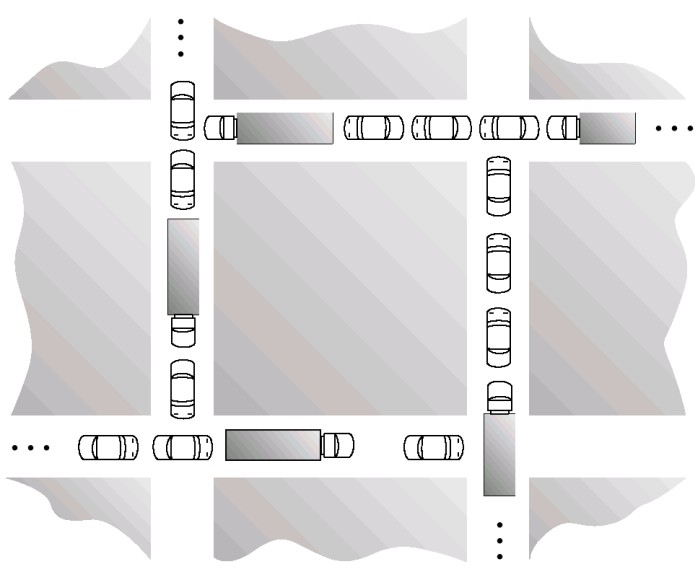
\includegraphics[scale=0.35]{figure/deadlock_car.jpg}
  \end{center}
\end{frame}


\begin{frame}[fragile]{若干死锁的例子}
  \begin{easylist} \easyitem
    & 例1进程推进顺序不当产生死锁
    && 设系统有打印机、读卡机各一台,被进程P和Q共享。两个进程并发执行,按下列
    次序请求和释放资源:
    \begin{center}
      \begin{columns}[T]
        \begin{column}{0.3\textwidth}
          \begin{tabular}{|c|}
            \hline
            进程P \\ \hline
            请求读卡机 \\
            请求打印机\\
            释放读卡机\\
            释放打印机 \\ \hline
          \end{tabular}
        \end{column}
        \begin{column}{0.3\textwidth}
          \begin{tabular}{|c|}
            \hline
            进程Q\\ \hline
            请求打印机\\
            请求读卡机\\
            释放读卡机\\
            释放打印机 \\ \hline
          \end{tabular}
        \end{column}
      \end{columns}
    \end{center}
  \end{easylist}
\end{frame}


\begin{frame}[fragile]{例2 PV操作使用不当产生死锁}
  \begin{center}
    \begin{columns}[T]
      \begin{column}{0.35\textwidth}
        \begin{tabular}{|c|}
          \hline 
          进程P \\ \hline
          $P(S_1)$; \\
          $P(S_2)$; \\
          使用资源$r_1$和$r_2$;\\
          $V(S_1)$; \\
          $V(S_2)$; \\ \hline
        \end{tabular}
      \end{column}
      \begin{column}{0.35\textwidth}
        \begin{tabular}{|c|}
          \hline 
          进程P \\ \hline
          $P(S_2)$; \\
          $P(S_1)$; \\
          使用资源$r_1$和$r_2$;\\
          $V(S_2)$; \\
          $V(S_1)$; \\ \hline
        \end{tabular}
      \end{column}
    \end{columns}
  \end{center}
\end{frame}

\begin{frame}[fragile]{例3 资源分配不当引起死锁}
  \begin{center}
    \begin{tikzpicture}[c/.style={draw,thick, minimum width=1cm, minimum height=0.6cm},
      c2/.style={draw,thick, shape=circle,inner sep=0.1cm, fill=red!20},
      b/.style={draw,thick, fill=black, shape=circle,minimum height=0.15cm, inner sep=0.02cm}]

      \draw[] node[c2] (p1) at(0,0) {$P_1$} 
      node[c2, right=1cm of p1] (p2) {$P_2$} 
      node[c2, right=1cm of p2] (p3) {$P_3$};

      \draw[] node[c] (r1) at(0.7,2) {} node[b] (b1) at(0.7,2) {}  node[above=0.1 of r1]{$R_1$}
      node[c] (r2) at (2.5,2) {} node[b] (b2) at(2.5,2) {}  node[above=0.1 of r2]{$R_2$}
      node[c,minimum height=1cm] (r3) at (0.7, -2) {}  node[b] (b3) at(0.7,-1.8) {}   node[b] (b4) at(0.7,-2.2) {}  node[below=0.1 of r3]{$R_3$}
      node[c,minimum height=1.2cm] (r4) at (2.6, -2.5) {}  node[b] (b5) at(2.6,-2.2) {}   node[b] (b6) at(2.6,-2.5) {}  node[b] (b7) at(2.6,-2.8) {}  node[below=0.1 of r4]{$R_4$};

      \path[-Stealth, thick] (p1) edge (r1) (b1) edge (p2) (p2) edge (r2) (b2) edge (p3)
      (b4) edge (p1) (b3) edge (p2) (p3) edge (r3);
    \end{tikzpicture}
  \end{center}
\end{frame}

\begin{frame}[fragile]{例4 对临时性资源使用不加限制引起死锁}
  \begin{easylist}
    & 进程通信使用的信件是一种临时性资源,如果对信件的发送和接收不加限制,可能引起死锁。
  \end{easylist}
  \begin{center}
    \begin{tikzpicture}[c/.style={draw,thick, minimum width=1cm, minimum height=0.6cm}]
      \draw[] node[] (p1) at(0:0) {$P_1$} node[] (p2) at (225:3) {$P_2$} node[] (p3) at (-45:3) {$P_3$};
      \path[->] (p1) edge node[left]{$send(P_2, S_1)$} (p2)
      (p2) edge node[below]{$send(P_3, S_2)$} (p3)
      (p3) edge node[right]{$send(P_1, S_3)$} (p1);
    \end{tikzpicture}
  \end{center}

   上图中,进程$P_1$需要接收到由$P_3$发送来的资源$S_3$后,就可以向进程$P_2$发送资源$S_1$ $...$
\end{frame}


\begin{frame}[fragile]{3.5.1 产生死锁的原因}
  \begin{enumerate}
  \item 竞争资源引起死锁
  \item 进程推进顺序不当引起死锁
  \end{enumerate}
\end{frame}

\begin{frame}[fragile]{1. 竞争资源引起死锁}
  \begin{easylist} \easyitem
    & 1.可剥夺(CPU、内存,)和非剥夺性(打印机,磁带机)资源
    & 2.竞争非剥夺性资源——可造成死锁 
  \begin{center}
    \begin{tikzpicture}[c/.style={draw, thick, fill=red!20, circle, inner sep=0.1cm}]
      \draw[] node[c] (p1) at(0:0) {$P_1$} node[c] (p2) at (-90:2) {$P_2$} node[draw, xshift=-0.5cm] (r1) at (-135:1.5) {$R_1$}  node[draw, xshift=0.5cm] (r2) at (-45:1.5) {$R_2$};
      \path[->] (p1) edge (r2) (r2) edge (p2) (p2) edge (r1) (r1) edge (p1);
    \end{tikzpicture}
  \end{center}
    & 3.竞争临时性资源
    && 永久性资源可重复使用,临时性资源是指由一个进程产生,被另一个进程使用一段
    时间后便无用的资源,也称为消耗性资源。
  \end{easylist}
\end{frame}


\begin{frame}[fragile]{2. 进程推进顺序不当引起死锁}
  \begin{easylist} \easyitem
    & 下图四种颜色的线表示了四种不同的推进顺序,其中红色线所代表的推进顺序会导致死锁
  \end{easylist}
  \begin{center}
    \small
    \begin{tikzpicture}[c/.style={draw,circle, inner sep=0.1cm}]
      \draw[thick] (-0.5, 0)--(9,0) (0,-0.2)--(0,5.5);
      \draw[dotted, thick] node[below] (p11) at (2,0) {$P_1: Req(R_1)$} (2,0)--(2,4.5);
      \draw[dotted, thick] node[below] (p12) at (4,0) {$P_1: Req(R_2)$} (4,0)--(4,4.5);
      \draw[thick] node[below] (p13) at (6,0) {$P_1: Rel(R_1)$} (6,0)--(6,0.75);
      \draw[thick] node[below] (p14) at (8,0) {$P_1: Rel(R_2)$} (8,0)--(8,0.75);

      \draw[dotted, thick] node[left] (p21) at (0,2) {$P_2: Req(R_2)$} (0,2)--(5.5,2);
      \draw[dotted, thick] node[left] (p22) at (0,3) {$P_2: Req(R_1)$} (0,3)--(8.5,3);
      \draw[thick] node[left] (p23) at (0,4) {$P_2: Rel(R_2)$} (0,4)--(0.2,4);
      \draw[thick] node[left] (p24) at (0,5) {$P_2: Rel(R_1)$} (0,5)--(0.2,5);

      \draw[line width=1.2pt, blue,->] (0.2, 0.5)--(8.5,0.5)--(8.5,5.5);
      \draw[line width=1.2pt, purple!90,->] (0.5, 0.2)--(0.5,5)--(8.7,5);
      \draw[line width=1.2pt,->] (0.75,0.75)--(5.5,0.75)--(5.5,2)--(8,2)--(8,5.2);
      \draw[line width=2pt,->, red] (0.75,0.75)--(0.75,1.5)--(3,1.5)--(3,2.5);
      \draw[->, red] node[shape=ellipse, draw=red, thick] (tip) at(5,4) {进入死锁} (3.1, 2.2)--(tip);
    \end{tikzpicture}
  \end{center}
\end{frame}


\begin{frame}[fragile]{3.5.2 产生死锁的必要条件}
  \begin{easylist} \easyitem
    & 1.互斥条件(Mutual Exclusion)
    && 共享资源不会导致死锁,如只读文件
    && 某些资源,如打印机、磁带等,需要被单个进程互斥访问
    & 2.请求和保持条件(Hold and Wait)
    && 持有等待
    & 3.不剥夺条件(No Preemption)
    && 不能抢占
    & 4.环路等待(Circular Wait)
    && 循环等待
  \end{easylist}
\end{frame}

\begin{frame}[fragile]{3.5.3 处理死锁的基本方法}
  \begin{easylist} \easyitem
    & 不允许死锁发生
    && 1.静态预防;
    &&& 破坏4个条件之一:有效,使资源利用率低。
    && 2.动态避免
    &&& 防止进入不安全态。
    & 允许死锁发生
    && 3. 顺其自然、不予理睬
    && 4.检测+解除:检测到死锁再清除。
  \end{easylist}
\end{frame}

\begin{frame}[fragile]{3.6 死锁预防和避免}
  \begin{easylist} \easyitem
    & 死锁预防
    && 破坏四个条件之一
    & 死锁避免
    && 通过银行家算法判断系统安全状态
  \end{easylist}
\end{frame}


\begin{frame}[fragile]{3.6.1 死锁预防}
  \begin{easylist} \easyitem
    & 一、互斥条件是资源固有属性,不能避免。
    & 二、摒弃请求和保持条件
    && 全分配,全释放(AND)
    && 缺点:(1) 延迟进程运行; (2) 资源严重浪费
    & 三、摒弃“不剥夺”条件
    && 增加系统开销,且进程前段工作可能失效。 
    & 四、摒弃“环路”条件
    && 有序资源分配法:为资源编号,申请时需按编号进行。
    && 缺点: (1) 新增资源不便(原序号已排定); (2) 用户不自由; (3) 资源与进程使用顺序不同造成浪费
  \end{easylist}
\end{frame}


\begin{frame}[fragile]{3.6.2 死锁避免之系统安全状态}
  \begin{easylist} \easyitem
    & 按某种顺序并发进程都能达到获得最大资源而顺序完成的序列为安全序列。
    & 能找到安全序列的状态为安全状态。
  \end{easylist}
\end{frame}

\begin{frame}[fragile]{安全状态举例}
  \begin{center}
    \begin{tabular}{|c|c|c|c|}
      \hline
      \rowcolor{yellow!30}
      进程 & 最大需求 & 已分配 & 可用 \\ \hline
      $P_1$ & 10 & 5 & 3 \\ \hline
      $P_2$ & 4 & 2 & ~ \\ \hline
      $P_3$ & 9 & 2 & ~ \\ \hline
    \end{tabular}

    安全序列:$P_2 \rightarrow P_1 \rightarrow P_3$
  \end{center}
\end{frame}

\begin{frame}[fragile]{安全状态向不安全状态的转换}
  \begin{easylist} \easyitem
    & 上例中,若P3再申请一台,则不安全
  \end{easylist}
  \begin{center}
    \begin{tabular}{|c|c|c|c|}
      \hline
      \rowcolor{yellow!30}
      进程 & 最大需求 & 已分配 & 可用 \\ \hline
      $P_1$ & 10 & 5 & {\color{red} 2} \\ \hline
      $P_2$ & 4 & 2 & ~ \\ \hline
      $P_3$ & 9 & {\color{red} 3} & ~ \\ \hline
    \end{tabular}
  \end{center}
\end{frame}


\begin{frame}[fragile]{3.6.3 利用银行家算法避免死锁}
  \begin{easylist} \easyitem
    & 1.数据结构
    && $available[j]=k$: 系统现有$R_j$类资源$k$个;
    && $max[i,j]=k$: 进程i需要$R_j$的最大数$k$个;
    && $alloc[i,j]=k$: 进程$i$已得到$R_j$类资源$k$个;   
    && $need[i,j]=k$: 进程$i$需要$R_j$类资源$k$个
    &&& $\therefore need[i,j]= max[i,j] - alloc[i,j]$
    && $request_i$: 进程$i$请求资源数
    && $work_i$:进程$i$执行完后系统应有资源数(也即可用数)
    && $finish[i]$:布尔量,表进程$i$能否顺序完成。
  \end{easylist}
\end{frame}


\begin{frame}[fragile]{示例}
  \begin{center}
    \newcolumntype{B}{>{\columncolor{yellow!10}}c}
    
    \begin{tabular}{|c| c c c | r c l  |r c l |r c l |}
      \Xhline{1.1pt}
      ~ &  \multicolumn{3}{|c|}{Max} &  \multicolumn{3}{|c|}{Allocation} &  \multicolumn{3}{|c|}{Need} &  \multicolumn{3}{|c|}{Available} \\ \cline{2-13}
      ~ & A & B & C  &  A & B & C & A & B & C  &  A & B & C \\ \Xhline{1pt}
      $P_0$ & 7 & 5 & 3   &   0 & 1 & 0    &    7 & 4 & 3    &   3 & 3 & 2 \\
            &   &   &     &     &   &      &      &   &      &  (2 & 3 & 0) \\ \cline{1-10}
      $P_1$ & 3 & 2 & 2   &   2 & 0 & 0    &    1 & 2 & 2    &   ~ & ~ & ~ \\
           &   &   &     &   (3 & 0 & 2)   &   (0 & 2 & 0)   &     &   &   \\ \cline{1-10}
      $P_2$ & 9 & 0 & 2   &   3 & 0 & 2    &    6 & 0 & 0    &     &   &   \\
           &   &   &     &     &   &      &      &   &       &     &   &   \\ \cline{1-10}
      $P_3$ & 2 & 2 & 2   &   2 & 1 & 1    &    0 & 1 & 1    &     &   &   \\
           &   &   &     &     &   &      &      &   &       &     &   &   \\ \cline{1-10}
      $P_4$ & 4 & 3 & 3   &   0 & 0 & 2    &    4 & 3 & 1    &     &   &   \\
           &   &   &     &     &   &      &      &   &       &     &   &   \\ 
      \Xhline{1.1pt}
    \end{tabular}

    $T_0$时刻的资源分配表
  \end{center}
\end{frame}


\begin{frame}[fragile]{示例}
 \begin{center}
    \begin{tabular}{|c| c c c | r c l  |r c l |r c l | c |}
      \Xhline{1.1pt}
      ~ &  \multicolumn{3}{|c|}{Work} &  \multicolumn{3}{|c|}{Need} &  \multicolumn{3}{|c|}{Allocation} &  \multicolumn{3}{|c|}{Work+Allocation} & Finish \\ \cline{2-13}
      ~     & A  & B & C   &   A & B & C    &    A & B & C    &    A & B & C & \\ \Xhline{1pt}
      $P_1$ &  3 & 3 & 2   &   1 & 2 & 2    &    2 & 0 & 0    &    5 & 3 & 2 & $\surd$ \\ \hline
      $P_3$ &  5 & 3 & 2   &   0 & 1 & 1    &    2 & 1 & 1    &    7 & 4 & 3 & $\surd$ \\ \hline
      $P_4$ &  7 & 4 & 3   &   4 & 3 & 1    &    0 & 0 & 2    &    7 & 4 & 5 & $\surd$ \\ \hline
      $P_2$ &  7 & 4 & 5   &   6 & 0 & 0    &    3 & 0 & 2    &   10 & 4 & 7 & $\surd$ \\ \hline
      $P_0$ & 10 & 4 & 7   &   7 & 4 & 3    &    0 & 1 & 0    &   10 & 5 & 7 & $\surd$ \\ 
      \Xhline{1.1pt}
    \end{tabular}

    $T_0$时刻的安全序列
  \end{center}
\end{frame}


\begin{frame}[fragile]{示例}
 \begin{center}
    \begin{tabular}{|c| c c c | r c l  |r c l |r c l | c |}
      \Xhline{1.1pt}
      ~ &  \multicolumn{3}{|c|}{Work} &  \multicolumn{3}{|c|}{Need} &  \multicolumn{3}{|c|}{Allocation} &  \multicolumn{3}{|c|}{Work+Allocation} & Finish \\ \cline{2-13}
      ~     & A  & B & C   &   A & B & C    &    A & B & C    &    A & B & C & \\ \Xhline{1pt}
      $P_1$ &  2 & 3 & 0   &   0 & 2 & 0    &    3 & 0 & 2    &    5 & 3 & 2 & $\surd$ \\ \hline
      $P_3$ &  5 & 3 & 2   &   0 & 1 & 1    &    2 & 1 & 1    &    7 & 4 & 3 & $\surd$ \\ \hline
      $P_4$ &  7 & 4 & 3   &   4 & 3 & 1    &    0 & 0 & 2    &    7 & 4 & 5 & $\surd$ \\ \hline
      $P_0$ &  7 & 4 & 5   &   7 & 4 & 3    &    0 & 1 & 0    &    7 & 5 & 5 & $\surd$ \\ \hline
      $P_2$ &  7 & 5 & 5   &   6 & 0 & 0    &    3 & 0 & 2    &   10 & 5 & 7 & $\surd$ \\ 
      \Xhline{1.1pt}
    \end{tabular}

    $P_1$申请资源(1,0,2)时安全性检查(安全)
  \end{center}
\end{frame}

\begin{frame}[fragile]{示例}
 \begin{center}
    \begin{tabular}{|c| c c c | r c l  |r c l |r c l | c |}
      \Xhline{1.1pt}
      ~ &  \multicolumn{3}{|c|}{Allocation} &  \multicolumn{3}{|c|}{Need} &  \multicolumn{3}{|c|}{Available} \\ \cline{2-10}
      ~     &  A & B & C   &   A & B & C    &    A & B & C   \\ \Xhline{1pt}
      $P_0$ &  0 & 3 & 0   &   7 & 2 & 3    &    2 & 1 & 0   \\ \cline{1-7}
      $P_1$ &  3 & 0 & 2   &   0 & 2 & 0    &      &   &     \\ \cline{1-7}
      $P_2$ &  3 & 0 & 2   &   6 & 0 & 0    &      &   &     \\ \cline{1-7}
      $P_3$ &  2 & 1 & 1   &   0 & 1 & 1    &      &   &     \\ \cline{1-7}
      $P_4$ &  0 & 0 & 2   &   4 & 3 & 1    &      &   &     \\ 
      \Xhline{1.1pt}
    \end{tabular}

    为$P_0$分配$(0, 2, 0)$后的情况(不安全)
  \end{center}
\end{frame}


\begin{frame}[fragile]{3.7 死锁的检测与解除}
  \begin{easylist} \easyitem
    & 3.7.1 死锁的检测
  \end{easylist}
\end{frame}

\begin{frame}[fragile]{3.7.1 死锁的检测}
  \begin{easylist} \easyitem
    & 1. 资源分配图
    & 2. 死锁定理
    & 3. 检测死锁的算法
  \end{easylist}
\end{frame}

\begin{frame}[fragile]{1. 资源分配图}
  \begin{center}
    \begin{tikzpicture}[c/.style={draw,thick, minimum width=1cm, minimum height=0.6cm},
      c2/.style={draw,thick, shape=circle,inner sep=0.1cm},
      b/.style={draw,thick, fill=black, shape=circle,minimum height=0.15cm, inner sep=0.02cm}]
      \draw[] node[c2] (p1) {$P_1$} 
      node[c2, below=2cm of p1] (p2) {$P_2$} 
      node[c, below left=1cm of p1,xshift=-1cm] (rg1) {}
      node[c, below right=1cm of p1,xshift=1cm] (rg2) {}
      node[b,below=-0.25cm of rg1] {} node[b,left=-0.3cm of rg1] {} node[b,right=-0.3cm of rg1] {}
      node[b,left=-0.4cm of rg2] {} node[b,right=-0.4cm of rg2] {};

      \path[->] (rg1.135) edge (p1.180) (rg1.60) edge (p1.210)
      (rg1.-120) edge (p2.180) (p2.150) edge (rg1.-60)
      (p1) edge (rg2) (rg2) edge (p2);
    \end{tikzpicture}
  \end{center}
\end{frame}

\begin{frame}[fragile]{2. 死锁定理}
  \begin{easylist} \easyitem
    & 简化资源分配图
    & 若能完全简化则消去所有的边
    & 定理:
    && 死锁状态的充分条件,资源分配图不可完全简化
  \end{easylist}
\end{frame}


\begin{frame}[fragile]{3. 检测死锁的算法}
  \begin{algorithm}[H]
    
    \caption{\label{alg:tree} \small 死锁检测算法}
    \begin{algorithmic}[1]
      \State work = available;
      \State $L = \{L_i | alloc_i=0, req_i=0 \}$ //孤立进程点
      \For{all $L_i \in L$}
        \For{all $req_i \leq work$}
          \State $work=work + alloc_i$
          \State $L=L_i \cup L$
        \EndFor
      \EndFor
      
      \State Deadlock = $\neg (L=\{p_1, \cdots, p_n\})$
    \end{algorithmic}
  \end{algorithm}

\end{frame}


\begin{frame}[fragile]{3.7.2 死锁的解除}
  \begin{easylist} \easyitem
    & 检测到死锁后,回退到上一状态(要进行资源剥夺,且需保存以前状态的分配信息),重新分配,若不行,继续回退……
    & 策略
    && 抢占资源
    && 杀死进程
    && 上翻:rollback
    && 难点:
    &&& 难以准确判断是否有死锁
    &&& 计算量大
    &&& 问题:检查死锁本身出问题
  \end{easylist}
\end{frame}


\begin{frame}[fragile]{讨论:如何应对死锁?}
  \begin{easylist} \easyitem
    & 检测修复与动态避免成本较高
    && 实现的程序复杂性
    && 运行时间
    & 综合治理
    && 对CPU、内存实施可抢占的静态防止策略(破坏不剥夺条件)
    && 对磁盘、打印机实施假脱机共享
    && 一些特殊资源按顺序访问
    && 剩余的其他问题不予理睬
  \end{easylist}
\end{frame}

\begin{frame}[fragile]{课堂作业}
  \begin{easylist} \easyitem
    & 设系统中有3种类型的资源(A,B,C)和5个进程P1、P2、P3、P4、P5。A资源的数量
    为17,B资源的数量为5,C资源的数量为20。在$T_0$时刻系统状态见下表所示。系统采用银
    行家算法实施死锁避免策略。
    & $T_0$时刻系统状态
  \end{easylist}

  \begin{center}
    \begin{tabular}{|c|c|c|c|c|c|c|}
      \hline
      &   \multicolumn{3}{|c|}{最大资源需求量} &  \multicolumn{3}{|c|}{已分配资源数量} \\  \cline{2-7}
      & ~~A~~ & ~~B~~ & ~~C~~ & ~~A~~ & ~~B~~ & ~~C~~ \\ \hline
      $P_1$ & 5 & 5 & 9 & 2 & 1 & 2 \\ \hline
      $P_2$ & 5 & 3 & 6 & 4 & 0 & 2 \\ \hline
      $P_3$ & 4 & 0 & 11 & 4 & 0 & 5 \\ \hline
      $P_4$ & 4 & 2 & 5 & 2 & 0 & 4 \\ \hline
      $P_5$ & 4 & 2 & 4 & 3 & 1 & 4 \\ \hline
    \end{tabular}
  \end{center}
\end{frame}

\begin{frame}[fragile]{问题}
  \begin{easylist} \easyitem
    & (1) $T_0$时刻是否为安全状态?若是,请给出安全序列。
    % 可以,存在安全序列$\{P_4, P_5, P_1, P_2, P_3\}$
    & (2) 在$T_0$时刻若进程$P_2$请求资源$(0,3,4)$,是否能实施资源分配?为什么?
    % 不能, Request(0,3,4) > Available(2,3,3)
    & (3) 在(2)的基础上,若进程$P_4$请求资源$(2,0,1)$是否能实施资源分配?为什么?
    % 可以,Request(2, 0, 1) < Available(2, 3, 3), 分配后存在安全序列$\{P_4, P_5, P_1, P_2, P_3\}$
    & (4) 在(3)的基础上,若进程$P_1$请求资源$(0,2,0)$是否能实施资源分配?为什么?
    % 不能,找不到安全序列
  \end{easylist}
\end{frame}


\begin{frame}[fragile, allowframebreaks]{复习题}
  \begin{enumerate}
  \item 如果系统中有n个进程,则在等待队列中进程的个数最多可为( {\color{white}n~~~})个
  \item 在操作系统中,不可中断执行的操作称为( {\color{white}原语})
  \item 在有m个进程的系统中出现死锁时,死锁进程的个数k应该满足的条件是(
    {\color{white}$2 \leq k \leq m$})
  \item 不让死锁发生的策略可以分为静态和动态两种,死锁避免属于( {\color{white}
      动态})
  \item 若使当前运行进程总是优先级最高的进程,则应该选择进程( {\color{white}高优先级优
      先调度})调度算法
  \item 在操作系统中引起进程调度的因素有:( {\color{white}进程正常终止})、({\color{white}进程异常终止 })、({\color{white} 阻塞})、({\color{white} 时
      间片用完})、({\color{white} 有高优先级进程})
  \item 产生进程死锁的根本原因是({\color{white}竞争资源 }),另一个基本原因是
    ({\color{white}进程推进顺序非法 }).
  \item 进程是一个程序对某个数据集的({\color{white}一次执行过程 })
  \item 在操作系统中引入线程的主要目的是({\color{white}降低进程切换开销 })
  \item 进程调度算法采用等时间片轮转法时,时间片过大,就会使轮转法转化为({\color{white}FCFS })调度算法
  \item 并发进程中涉及到相同变量的程序段叫做({\color{white}临界区 }),对这些程序段要({\color{white}互斥 })执行。
  \item 死锁产生的四个必要条件是:互斥控制、({\color{white} }请求和保持)、
    ({\color{white}不剥夺 })、({\color{white}环路等待 })。
  \item 某程序运行时经常要打印中间结果。计算时,该进程处于({\color{white} 执
      行})态,打印时处于({\color{white} 阻塞})态,打印结束时进程处于
    ({\color{white} 就绪})态。
  \item 操作系统中,可以并行工作的基本单位是({\color{white}进程 }),它是由程
    序、({\color{white} 数据})和({\color{white}PCB })组成。
  \item 进程初建时处于({\color{white}就绪 })态,运行时因为时钟中断而处于
    ({\color{white} 就绪})态,因等事件或资源而处于({\color{white}阻塞 })态
  \item 当处理机空闲时,进程调度程序从({\color{white}就绪 })队列中选取一个进程执行。
  \item 当采用静态资源分配法预防死锁时,破坏了产生死锁的四个必要条件中的
    ({\color{white}请求和保持 })条件。
  \end{enumerate}
\end{frame}

\begin{frame}[fragile]{作业}
  \begin{enumerate}
  \item CPU与GPU
  %\item 开源软件简史 \footnote{\url{https://linuxstory.org/simple-history-about-opensource-1/}}
  \end{enumerate}
\end{frame}

%%% Local Variables:
%%% mode: latex
%%% TeX-master: "../os"
%%% End:

%\section{存储管理}

\begin{frame}[fragile]{新问题}
  \begin{easylist}  \easyitem
    & 通过进程管理,OS可以控制管理程序的运行,并通过处理机调度,决定要哪一个程序
    运行。
    & 现代计算机的体系架构要求程序要读入内存才可以运行
    & \color{red}那怎么为进程分配存储空间呢?
  \end{easylist}

  \begin{center}
    \color{red} \huge --- 存储管理!  
  \end{center}
\end{frame}


\begin{frame}[fragile]{CH4 存储管理}
  \begin{easylist} \easyitem
    & 4.0 引言
    & 4.1 程序的装入和运行
    & 4.2 连续分配方式
    & 4.3 基本分页存储管理方式
    & 4.4 基本分段存储管理方式
    & 4.5 虚拟存储器的基本概念
    & 4.6 请求分页存储管理方式
    & 4.7 页面置换算法
    & 4.8 请求分段存储管理方式
  \end{easylist}
\end{frame}



\subsection{引言}

\begin{frame}[fragile]{4.0 引言}
  \begin{easylist} 
    & CPU不能直接存取外存上的信息
    && [1] 内存:
    &&& 是指CPU能直接存取指令和数据的存储器。CPU和I/O系统都要和内存打交道,对内存的访问是通过一系列对指定地址单元进行读或写来实现的。
    && [2] 高速缓存
    &&& CACHE由硬件寄存器构成,CPU可直接存取其中的信息,存取速度远大于内存。
    CACHE直接做在CPU中。
    &&& L1高速缓存也叫一级高速缓存,主要用于暂存CPU指令和数据
    &&& L2高速缓存也叫二级缓存,主要用于存放电脑运行时操作系统的指令、程序数据和地址指针等
  \end{easylist}
\end{frame}


\begin{frame}[fragile]{数据从设备到CPU}
  \begin{center} 
    \begin{tikzpicture}[c/.style={draw,thick, minimum width=2cm, minimum height=0.75cm}]
      \draw[] node[c] (cpu) {CPU} 
      node[c, right=0.5 of cpu] (memory) {内存}
      node[c, right=0.5 of memory] (io) {I/O系统}
      node[c, rounded corners, above right=0.8 of io] (d1) {外部设备}
      node[c, rounded corners,right=0.5 of io] (d2) {外部设备}
      node[c, rounded corners,below right=0.8 of io] (d3) {$\cdots$}
      ;
      \draw[<->] (cpu)--(memory);
      \draw[<->] (memory)--(io);
      \draw[<->] (io.10)--(d1);
      \draw[<->] (io)--(d2);
      \draw[<->] (io.-10)--(d3);
    \end{tikzpicture}
  \end{center}
\end{frame}


\begin{frame}[fragile]{三级存储器结构}
  \begin{center} 
    \begin{tikzpicture}[c/.style={draw,thick, minimum width=2cm, minimum height=0.75cm},
      c2/.style={draw, align=center, fill=blue!5, dotted}]
      \draw[] node[c, fill=yellow!10] (cache) {高速缓存器} 
      node[c, below=0.7 of cache] (memory) {内存}
      node[c, below=0.7 of memory] (disk) {外存}
      ;
      \path[<->] (cache) edge (memory) (memory) edge (disk);

      \draw[->, thick, color=red!50] (-1.5cm, -3.5cm) -- (-1.5cm,0.7cm);

      \draw[] node[left=of disk] (t1){存储器容量减少}
      node[above=0.5 of t1] (t2) {每位存储器成本增加}
      node[above=0.5 of t2] (t3) {存储器存取速度增加}
      node[above=0.5 of t3] {存储器存取时间减少};

      \draw[] node[c2, right=of cache, yshift=-0.4cm] (t4) {程序和数据\\可以被CPU\\直接存取};
      \draw[] node[c2, right=of disk, yshift=0.5cm] (t5) {程序和数据\\必须先移到\\内存,才能\\被CPU存取
      };
      \path[->] (cache.east) edge[bend left=30] (t4.west)
      (memory.east) ++(0,0.1) edge[bend right=30] (t4.west)
      (memory.east) edge[bend left=30] (t5.west)
      (disk.east) ++(0,-0.1) edge[bend right=30] (t5.west);
    \end{tikzpicture}
  \end{center}
\end{frame}


\begin{frame}[fragile]{存储器的层次结构}
  \begin{center}
    \scalebox{0.8}{
      \begin{tikzpicture}[c/.style={draw,thick, minimum height=0.75cm, fill=red!5},
        a/.style={thick, -Latex}]
        \draw[] node[c, minimum width=2cm] (cpu) {Registers} 
        node[c, below=0.5 of cpu, minimum width=3cm] (cache) {Cache} 
        node[c, below=0.5 of cache, minimum width=4cm] (ram) {Main memory}
        node[c, below=0.5 of ram, minimum width=5cm] (ssd) {Solid-state disk}
        node[c, below=0.5 of ssd, minimum width=6cm] (cipan) {magnetic disk}
        node[c, below=0.5 of cipan, minimum width=7cm] (guangpan) {optical disk}
        node[c, below=0.5 of guangpan, minimum width=8cm] (cidai) {magnetic tapes}
        ;
        \path[a,color=blue, fill=blue] (cpu.240) edge (cache.120)
        (cache.240) edge (ram.120) 
        (ram.240) edge (ssd.120) 
        (ssd.240) edge (cipan.120) 
        (cipan.240) edge (guangpan.120) 
        (guangpan.240) edge (cidai.120) ;
        \path[a, color=red, fill=red]  (cache.70) edge (cpu.-70)
        (ram.70) edge (cache.-70)
        (ssd.70) edge (ram.-70)
        (cipan.70) edge (ssd.-70)
        (guangpan.70) edge (cipan.-70)
        (cidai.70) edge (guangpan.-70);
      \end{tikzpicture}
    }
  \end{center}
\end{frame}

\subsection{4.1 程序的装入和链接 }
\begin{frame}[fragile]{4.1 程序的装入和链接 }
  \begin{easylist} 
    & 编辑 $\rightarrow$ 编译  $\rightarrow$ 链接  $\rightarrow$ 装入
    $\rightarrow$ 运行
  \end{easylist}
  \begin{center}
    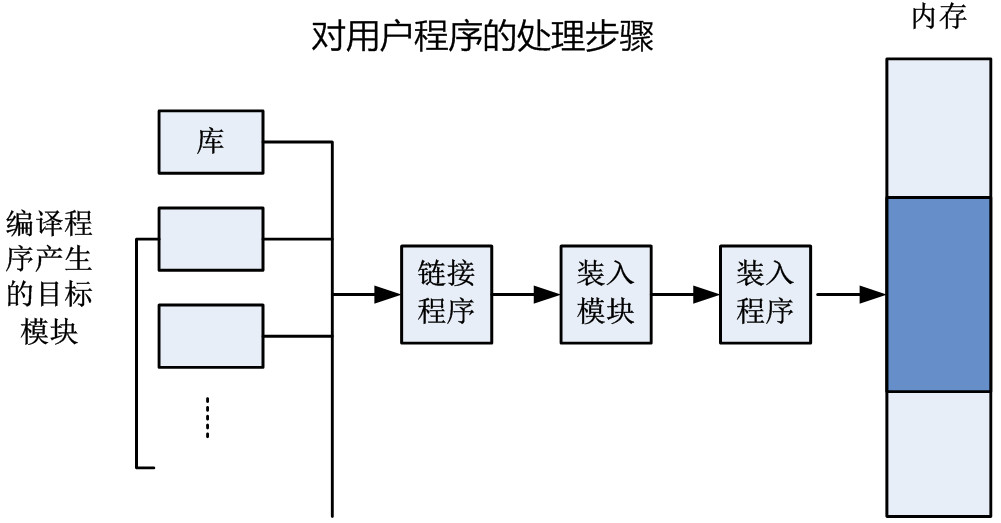
\includegraphics[width=0.9\textwidth]{figure/mem_link1.jpg}
  \end{center}
\end{frame}


\begin{frame}[fragile]{4.1.1 程序的装入 }
  \begin{easylist} 
    & 1、绝对装入(Absolute Loading Mode)
    && 编译后,装入前已产生了绝对地址(内存地址),装入时不再作地址重定位。
    && 绝对地址的产生:
    &&& (1) 由编译器完成
    &&& (2) 由程序员编程完成
    &&& 对(1)而言,编程用符号地址
    &&& 对(2)而言,要求程序员熟悉内存的使用情况,程序或数据修改后,可能要改变程序的原内存地址
  \end{easylist}
\end{frame}


\begin{frame}[fragile]{4.1.1 程序的装入 }
  \begin{easylist} 
    && 绝对装入的问题
    &&& 只能将目标模块装入到内存中事先指定的位置。在多道程序环境下,编译程序不可能预知所编译的目标模块应放在内存的何处,因此,只适用于单道程序环境。
  \end{easylist}
\end{frame}


\begin{frame}[fragile]{4.1.1 程序的装入}
  \begin{easylist} 
    & 2、可重定位装入(Relocation Loading Mode)
    && 装入时完成,主要工作是对相对地址中的指令和数据地址的调整过程,见图2
    && 地址变换通常是在装入时一次完成的,以后不再改变,故称为{\color{red}静态重定位}
    && 问题:
    &&& 不允许程序运行时在内存移动位置,但在实际运行过程中在内存中的位置要经常改变。
    &&& $\rightarrow$ 动态运行时装入方式
  \end{easylist}
\end{frame}



\begin{frame}[fragile]{作业装入内存的情况}
  \begin{center}
    \begin{tikzpicture}[c/.style={},
      a/.style={thick, -Latex}]

      \draw[thick] (0,0)--++(3,0) -- ++(0,-5)--++(-3,0)--++(0,5) ++(0,-1)--++(3,0)
      ++(0,-0.5)--++(-3,0) ++(0,-1)--++(3,0) ++(0,-0.5)--++(-3,0);

      \draw node[c] at(-0.2,0) {0} node[c] at(-0.5,-1) {1000} node[c] at(-0.5,-2.5) {2500} node[c] at(-0.5,-5) {5000} node at(1.5,-1.25) {LOAD 1, 2500};


      \draw[dotted, thick] (6,0)--++(0,1)--++(3,0)--++(0,-1);
      \draw[] (6,0)--++(3,0) -- ++(0,-5)--++(-3,0)--++(0,5) ++(0,-1)--++(3,0)
      ++(0,-0.5)--++(-3,0) ++(0,-1)--++(3,0) ++(0,-0.5)--++(-3,0);
      \draw[dotted, thick] (6,-5)--++(0,-1)--++(3,0)--++(0,1);

      \draw node[c] at(5.5,0) {10000} node[c] at(5.5,-1) {11000} node[c] at(5.5,-2.5) {12500} node[c] at(5.5,-5) {15000} node at(7.5,-1.25) {LOAD 1, 2500};
      
      \draw[thick, red!50, -Latex] (3,0)--(5,0);
      \draw[thick, red!50, -Latex] (3,-5)--(5,-5);

      \draw node at(1.5,-6) {作业地址空间} node at(7, -6) {内存空间};
    \end{tikzpicture}
  \end{center}
\end{frame}


\begin{frame}[fragile]{4.1.1 程序的装入 }
  \begin{easylist} 
    & 3.动态运行时装入
    && (Dynamic Run-time Loading)
    && 把装入模块装入内存时,并不立即把模块中的相对地址转换为绝对地址,而是推迟到程序真正要执行时才进行
    && 装入内存后的所有地址仍是相对地址
    && 一般在执行时才完成相对地址到绝对地址的转换,且有硬件的支持,能保证进程的可移动性。
  \end{easylist}
\end{frame}


\begin{frame}[fragile]{4.1.2 程序的链接}
  \begin{easylist} 
    & 1、静态链接(Static Linking)
    && a.对相对地址的修改
    && b.变换外部调用符号
    & 2、装入时动态链接(Load-time Dynamic Linking)
    && a.便于修改和更新
    && b.便于实现对目标模块的共享
    && e.g. DLL动态链接库
    & 3、运行时动态链接(Run-time Dynamic Linking)
    && e.g. Java Class Loader
  \end{easylist}
\end{frame}


\begin{frame}[fragile]{目标模块与装入模块示例}
  \begin{center}
    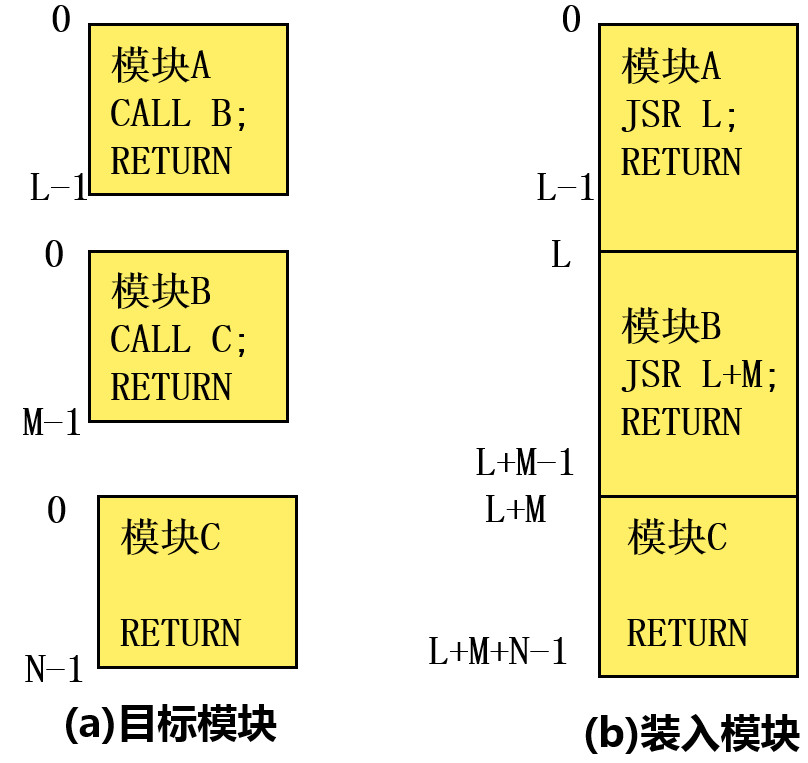
\includegraphics[width=0.6\textwidth]{figure/mem_link2.jpg}
  \end{center}
\end{frame}



\subsection{4.2 连续分配方式 }
\begin{frame}[fragile]{4.2 连续分配方式 }
  \begin{easylist} 
    & 4.2.1 单一连续分配
    && 用于单用户,单任务中
    & 4.2.2 固定分区分配
    & 4.2.3 动态分区分配
    & 4.2.4 可重定位分区分配
    & 4.2.5 对换
  \end{easylist}
\end{frame}



\begin{frame}[fragile]{4.2.1 单一连续分区}
  \begin{easylist} 
   & 最简单的存储管理方式,用于单用户、单任务OS
   & 内存划分为两部分:
   && 系统区:供OS使用,一般放在低址部分,Solaris则相反
   && 用户区
   & 存贮保护机构的设置
   && 一般不设置保护也可,因单任务运行。
   && 例如: MS-DOS, CP/M, RT-11            
  \end{easylist}
\end{frame}


\begin{frame}[fragile]{4.2.2 固定分区}
  \begin{easylist} 
  & 特点:有n个分区,则可同时装入n个作业/任务。
  & 一、分区大小:
  && 相等:
  && 不相等:不相等利用率更高。
  & 二、内存分配:
  && 数据结构: 固定分区使用表  
  &&& 将分区按大小排序,并将其地址、分配标识作记录
  & 三、特点:
  && 简单,有碎片(内零头)
  \end{easylist}
\end{frame}


\begin{frame}[fragile]{固定分区使用表}
  \begin{columns}[onlytextwidth,T]
    \begin{column}{0.5\textwidth}
      \begin{tabular}{|c|c|c|c|}
        \hline
        分区号 & 大小(k) & 起址(k) & 状态 \\ \hline
        1  & 12 & 20 & 已分配 \\ \hline
        2 & 32 & 32 & 已分配 \\ \hline
        3 & 64 & 64 & 已分配 \\ \hline
        4 & 128 & 128 & 已分配 \\ \hline
      \end{tabular}
    \end{column}

    \begin{column}{0.5\textwidth}
      \begin{tikzpicture}[c/.style={draw,thick, minimum width=2.5cm},
        tip/.style={yshift=0.2cm}]
        \small
        \draw[minimum height=1cm] node[c] (os) {操作系统}
        node[c,below=0 of os, minimum height=0.3cm, fill=yellow!60, dotted] {作业A} 
	node[c, below=0 of os, minimum height=0.8cm] (a) {}
        node[c,below=0 of a, minimum height=1cm, fill=yellow!60, dotted] {作业B} 
	node[c, below=0 of a, minimum height=1.6cm] (b) {}
        node[c,below=0 of b, minimum height=1.8cm, fill=yellow!60, dotted] {作业C} 
	node[c, below=0 of b, minimum height=2.5cm] (c) {}
        node[c, below=0 of c, minimum height=0.5cm] {$\cdots$};

        \draw[] node[below left=0 of os, tip] {20k}
        node[below left=0 of a, tip] {32k}
        node[below left=0 of b, tip] {64k}
        node[below left=0 of c, tip] {128k};
        \draw node[draw, shape=ellipse, dashed, inner sep=0cm, left=of c,minimum height=0.7cm, fill=red!15] (t) {内零头碎片};

        \path[-Latex] (t) edge (a.190) (t) edge (b.200) (t) edge (c.215);
      \end{tikzpicture}
    \end{column}
  \end{columns}
\end{frame}


\begin{frame}[fragile]{4.2.3 动态分区分配}
  \begin{easylist} 
    & 动态分区分配是根据进程的实际需要,动态为之分配内存空间。
    & 为实现动态分区分配,系统中必须配置相应的数据结构,用来描述空闲分区和已分配分区的情况。通常采用两种形式:
    && 空闲分区表
    && 空闲分区链
  \end{easylist}
\end{frame}


\begin{frame}[fragile]{一、动态分区分配的数据结构}
  \begin{easylist} 
  & 1 空闲分区表:记录每个空闲分区情况,表目包括:分区序号、分区始址及分区大小等.
  & 2 空闲分区链
  \begin{center}
    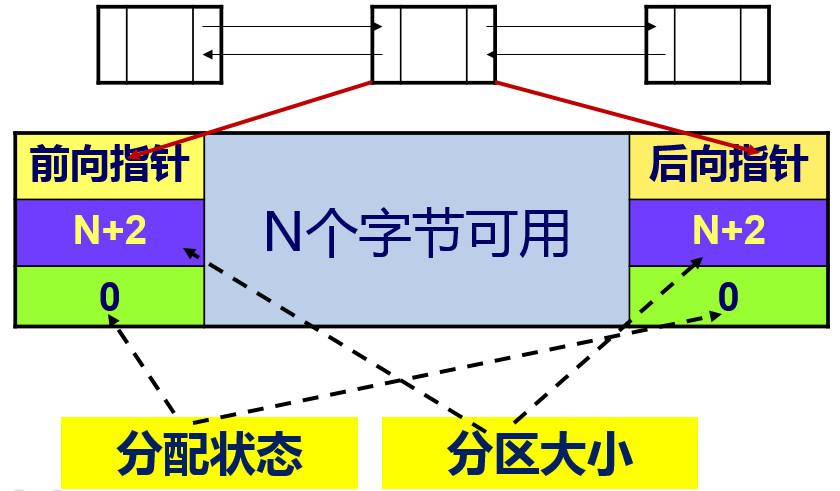
\includegraphics[width=0.6\textwidth]{figure/mem_fix1.jpg}
  \end{center}
  \end{easylist}
\end{frame}



\begin{frame}[fragile, allowframebreaks]{二、分区分配算法}
  \begin{easylist} 
    & 1 首次适应算法FF
    && 空闲区链:首址递增排列;
    && 申请:按分区的先后次序,从头查找,找到符合要求的第一个分区;
    && 优点:尽量使用低地址空间,高地址空间保持大的空闲区域。
    && 缺点:随着低地址分区不断划分而产生较多小分区(内存碎片),每次分配时查找
    时间开销会增大。

    \newpage
    & 2 循环首次适应算法
    && 空闲区链:首址递增排列;
    && 申请:从上次分配的分区起查找(到最后分区时再回到开头),找到符合要求的第一个分区,应设置一个查询指针。
    && 特点: 
    &&& 空闲分区分布均匀;
    &&& 大的空闲分区不易保留;
    &&& 查找时间开销会减小。

    \newpage
    & 3 最佳适应算法
    && 空闲区链:不是首址,而是分区容量递增排列;
    && 申请:找到符合要求的第一个分区。
    && 特点:碎片较小,但从整体来看,会形成较多的碎片。

    \newpage
    & 4 最差适应算法
    && 空闲区链:分区容量递减排列;
    && 申请:找到符合要求的第一个分区。
    && 特点:可以充分使用大的分区,但大的空闲分区不易保留。
  \end{easylist}
\end{frame}


\begin{frame}[fragile]{三、分区分配}
  \begin{easylist} 
    & 分配流程
    & 内存回收
  \end{easylist}
\end{frame}


\begin{frame}[fragile]{分配流程}
  \begin{center}
    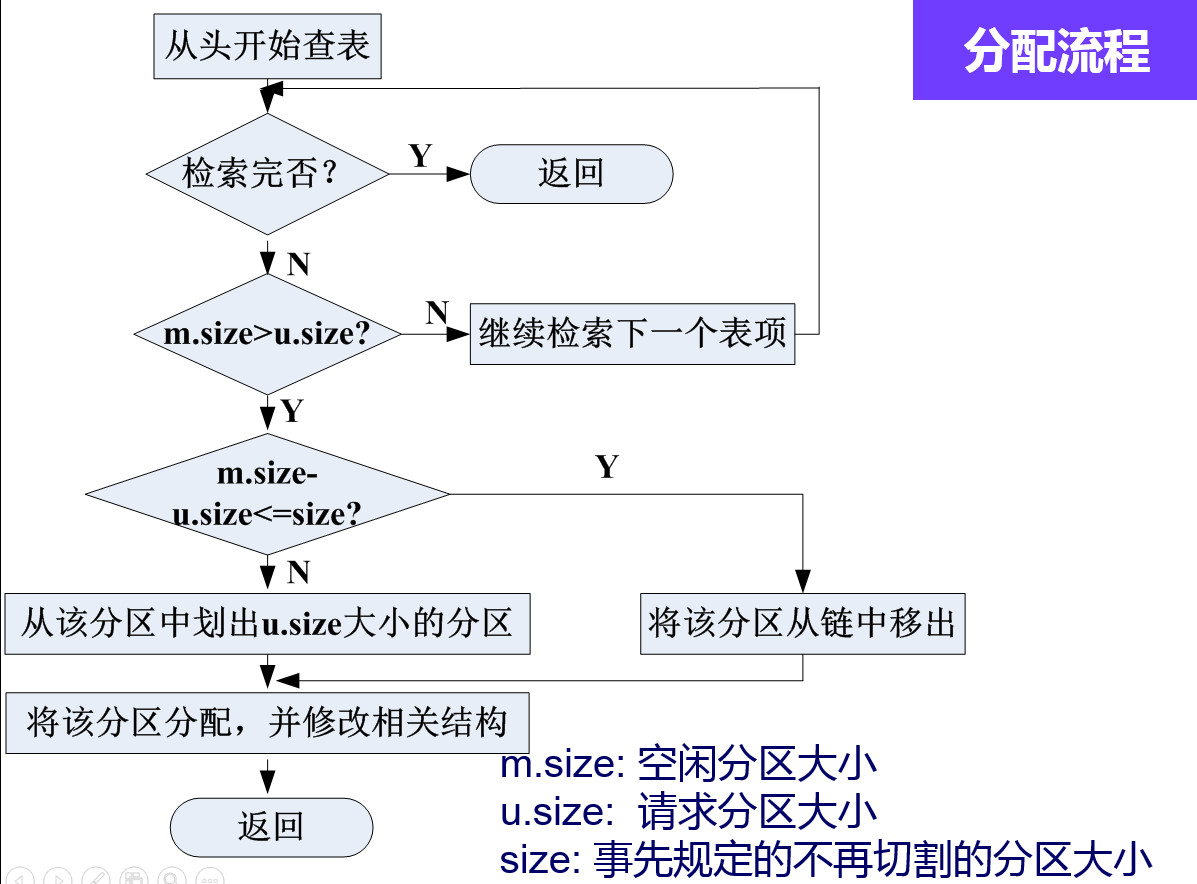
\includegraphics[width=0.8\textwidth]{figure/mem_fix2.jpg}
  \end{center}
\end{frame}


\begin{frame}[fragile]{内存回收}
  \begin{enumerate}
  \item 上邻空闲区:合并,改大小
  \item 下邻空闲区:合并,改大小,首址。
  \item 上、下邻空闲区:合并,改大小。
  \item 不邻接,则建立一新表项。
  \end{enumerate}
\end{frame}


\begin{frame}[fragile]{内存回收时的4种情况}
  \begin{center} 
    \begin{tikzpicture}[c/.style={draw,thick, minimum width=2cm, minimum height=1cm}]
      \draw[] node[c,fill=yellow!70](b1) {Free 1} 
      node[c, below=0 of b1, fill=orange!50] (b2) {回收区} 
      node[c, below=0 of b2, fill=gray!80] (b3) {Job B};
      
      \draw[] node[c,fill=yellow!70](b1) {Free 1} 
      node[c, below=0 of b1, fill=orange!50] (b2) {回收区} 
      node[c, below=0 of b2, fill=gray!80] (b3) {Job B};

      \draw[] node[c,fill=gray!80, right=of b1](b1) {Job A} 
      node[c, below=0 of b1, fill=orange!50] (b2) {回收区} 
      node[c, below=0 of b2, fill=yellow!70] (b3) {Free 2};

      \draw[] node[c,fill=yellow!70, right=of b1](b1) {Free 1} 
      node[c, below=0 of b1, fill=orange!50] (b2) {回收区} 
      node[c, below=0 of b2, fill=yellow!70] (b3) {Free 2};

      \draw[] node[c,fill=gray!80, right=of b1](b1) {Job A} 
      node[c, below=0 of b1, fill=orange!50] (b2) {回收区} 
      node[c, below=0 of b2, fill=gray!80] (b3) {Job B};
    \end{tikzpicture}
  \end{center}
\end{frame}



\begin{frame}[fragile]{课堂练习}
  \begin{easylist} 
  & 某系统采用动态分区分配方式管理内存,内存空间为640K,高端40K存放操作系统。在内
  存分配时,系统优先使用空闲区低端的空间。对下列请求序列:
  && 作业1申请130K、作业2申请60K、作业3申请100K
  && 作业2释放60K、作业4申请200K、作业3释放100K
  && 作业1释放130K、作业5申请140K、作业6申请60K
  && 作业7申请50K、作业6释放60K
  & 请分别画图表示出使用首次适应算法和最佳适应算法进行内存分配和回收后内存的实际使用情况。
  \end{easylist}
\end{frame}


\begin{frame}[fragile]{4.2.4 可重定位分区分配}
  \begin{easylist} 
  & 1 动态重定位的引入
  && 连续式分配中,总量大于作业大小的多个小分区不能容纳作业。
  && 紧凑
  &&& 通过作业移动将原来分散的小分区拼接成一个大分区。
  &&& 作业的移动需重定位。对程序和数据地址加以修改,以确保继续正常运行
  \end{easylist}
\end{frame}

\begin{frame}[fragile]{紧凑的示意}
  \begin{center}
    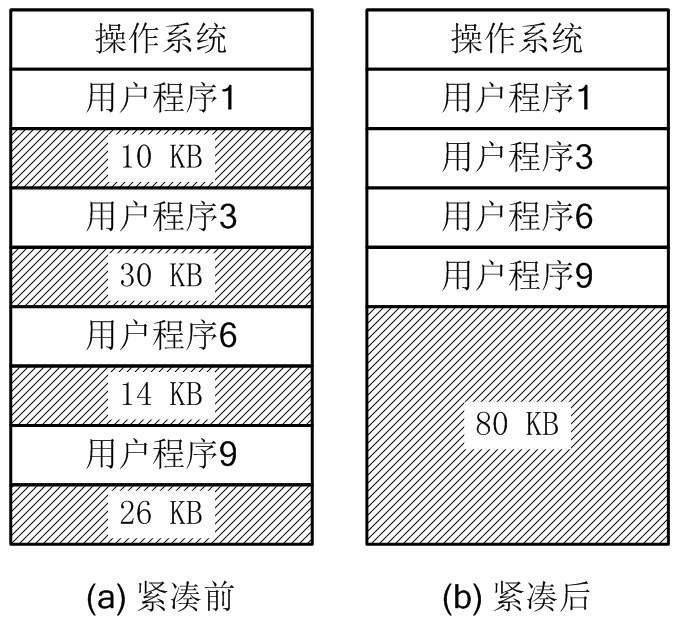
\includegraphics[width=0.6\textwidth]{figure/mem_fix_jincou.jpg}
  \end{center}
\end{frame}


\begin{frame}[fragile]{2 动态重定位的实现}
  \begin{center}
    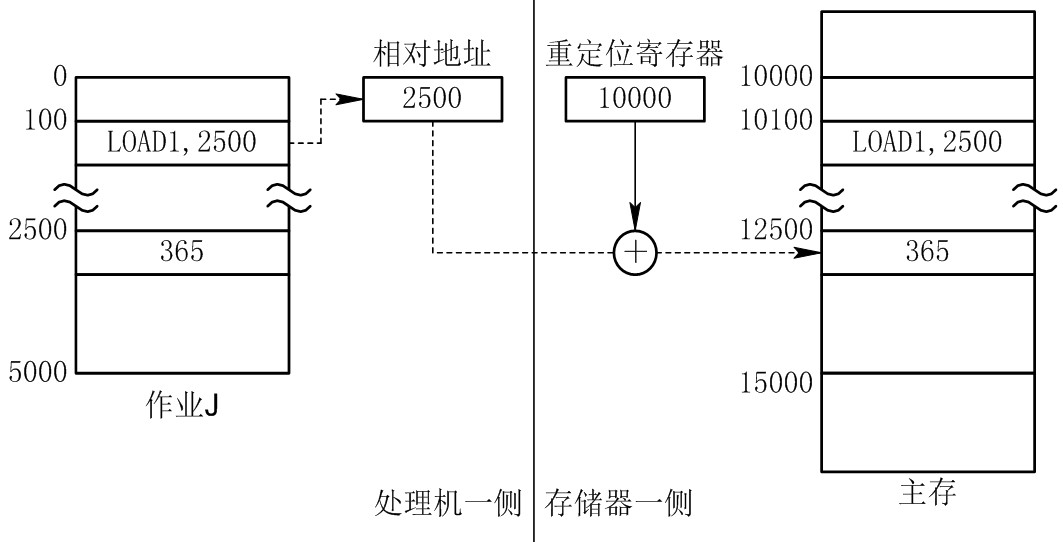
\includegraphics[width=0.9\textwidth]{figure/mem_fix_cdw.jpg}
  \end{center}
  \begin{easylist} 
   & 紧凑后,只需置换使用新起始地址即可
  \end{easylist}
\end{frame}


\begin{frame}[fragile]{动态分区分配算法流程图 }
  \begin{center}
    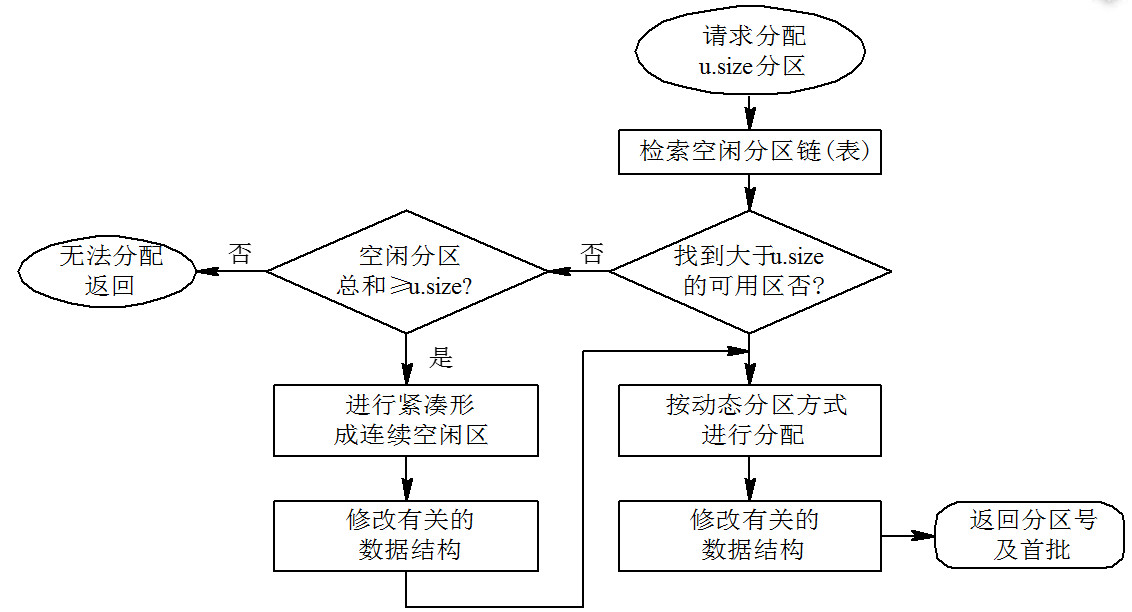
\includegraphics[width=1.0\textwidth]{figure/mem_fix_cdwlc.jpg}
  \end{center}
\end{frame}


\begin{frame}[fragile]{4.2.5 对换(Swapping)}
  \begin{easylist}
    \begin{enumerate}
      \item 对换的引入
      \item 对换空间的管理
      \item 进程的换出与换入
    \end{enumerate}
  \end{easylist}
\end{frame}


\begin{frame}[fragile]{1. 对换的引入}
  \begin{easylist} 
    & 在多道程序环境下,可以将暂时不能执行的程序送到外存中,从而获得空闲内存空间来装入新程序。
    & 所谓“对换”,是指把内存中暂时不能运行的进程或者暂时不用的程序和数据,调出
    到外存上,以便腾出足够的内存空间,再把已具备运行条件的进程或进程所需要的程序
    和数据,调入内存。对换是提高内存利用率的有效措施。
    & 如对换以整个进程为单位,称为“整体对换”或“进程对换”,广泛应用于分时系统中;
    如以“页”或“段”为单位,称为“页面对换”或“分段对换”
  \end{easylist}
\end{frame}

\begin{frame}[fragile]{对换的优缺点}
  \begin{easylist} 
   & 优点:
   && 增加并发运行的程序数目,并且给用户提供适当的响应时间;编写程序时不影响程序结构。
   & 缺点:
   && 对换入和换出的控制增加了处理机开销;
  \end{easylist}
\end{frame}


\begin{frame}[fragile]{2. 对换空间的管理}
  \begin{easylist} 
   & 把外存分为文件区和对换区。对换区用来存放从内存换出的进程。主要目标是提高进程换入和换出的速度。
   & 为了能对对换区中的空闲盘块进行管理,在系统中应配置相应的数据结构,以记录外存的使用情况。其形式与内存在动态分区分配方式中所用数据结构相似,即同样可以用空闲分区表或空闲分区链。在空闲分区表中的每个表目中应包含两项, 即对换区的首址及其大小,它们的单位是盘块号和盘块数。
  \end{easylist}
\end{frame}


\begin{frame}[fragile]{Linux下的对换空间使用情况举例}
  \begin{center}
    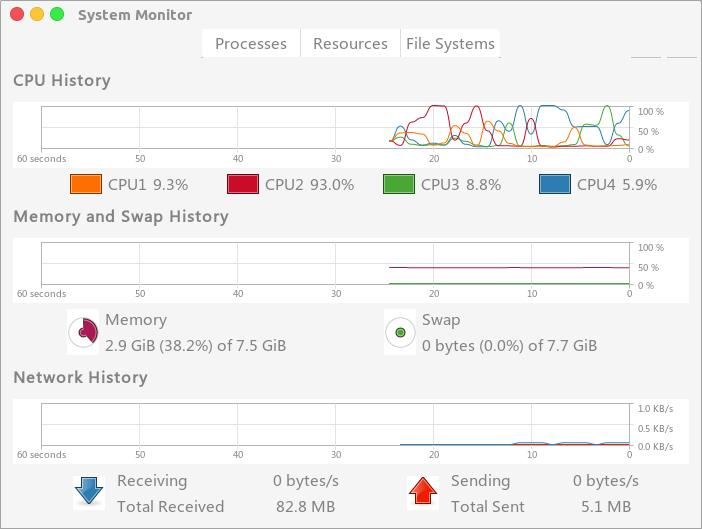
\includegraphics[width=0.8\textwidth]{figure/mem_swap_linux.jpg}
  \end{center}
\end{frame}

\begin{frame}[fragile]{Linux交换分区的大小设置建议}
  \begin{easylist} 
  & 基本原则:
  && 交换分区为内存大小的2倍
  && 交换分区不宜过大,如果内存大于2G,可以设为内存大小+2G
  && 例如:
  &&& 内存为512M,可以设为1G
  &&& 内存为4G,可以设为6G
  \vspace{1cm}
  &&& 如果内存很大的话,也可以不使用交换分区,前提是保证所有运行的程序内存总和不会超过实际内存大小
  \end{easylist}
\end{frame}


\begin{frame}[fragile]{3. 进程的换出与换入}
  \begin{easylist} 
    & 进程的换出。 
    && 每当一进程由于创建子进程而需要更多的内存空间,但又无足够的内存空间等情况发生时,系统应将某进程换出。 
    && 其过程是:系统首先选择处于阻塞状态且优先级最低的进程作为换出进程,然后启动盘块,将该进程的程序和数据传送到磁盘的对换区上。若传送过程未出现错误,便可回收该进程所占用的内存空间,并对该进程的进程控制块做相应的修改。 
    & 进程的换入
    && 系统应定时地查看所有进程的状态,从中找出“就绪”状态但已换出的进程,将其中换出时间(换出到磁盘上)最久的进程作为换入进程,将之换入,直至已无可换入的进程或无可换出的进程为止。
  \end{easylist}
\end{frame}


\begin{frame}[fragile]{PART2: 离散分配方式}
  \begin{easylist} 
  & 连续分配方式会形成许多碎片,虽然通过“紧凑”可以拼接,但是必须付出很多开销。因
  此产生了离散分配方式:
  && 分页
  && 分段
  && 段页
  \end{easylist}
\end{frame}


\subsection{4.3 基本分页存储管理方式}
\begin{frame}[fragile]{4.3 基本分页存储管理方式}
  \begin{easylist} 
   & 4.3.1 页面与页表
   & 4.3.2 地址变换机构
   & 4.3.3 两级或多级页表
  \end{easylist}
\end{frame}


\begin{frame}[fragile]{4.3.1 页面与页表 --- 页面}
  \begin{easylist} 
    & 1. 页面
    && 页面和物理块:逻辑空间和内存空间
    && 页面大小
    &&& 页太大,页内碎片大。
    &&& 页太小:页表可能很长,换入/出效率低
  \end{easylist}
\end{frame}

\begin{frame}[fragile]{页面和物理块}
  \begin{easylist} 
    & 分页存储管理,是将一个进程的逻辑地址空间分成若干个大小相等的片,称为页面或
    页,并为各页加以编号,从0开始,如第0页、第1页等。
    & 相应地,也把内存空间分成与页面相同大小的若干个存储块,称为(物理)块或页框
    (frame), 也同样为它们加以编号,如\#0、\#1等等。
    & 在为进程分配内存时,以块为单位将进程中的若干个页分别装入到多个可以不相邻接
    的物理块中。由于进程的最后一页经常装不满一块而形成了不可利用的碎片,称之为
    “页内碎片”。 
  \end{easylist}
\end{frame}


\begin{frame}[fragile]{页面大小的选择}
  \begin{easylist} 
    & 在分页系统中的页面其大小应适中。
    & 页面小:
    && 内存碎片减小,提高内存利用率
    && 每个进程占用较多页面,进程的页表过长,占用大量内存;
    && 降低页面换进换出的效率。
    & 页面大:
    && 减少页表长度,提高换进换出速度
    && 页内碎片增大
    & 页面的大小应选择应适中,且页面大小应是2的幂,通常为512B $\sim$ 8KB
  \end{easylist}
\end{frame}


\begin{frame}[fragile]{4.3.1 页面与页表 --- 地址结构}
  \begin{easylist} 
    & 2. 地址结构
    \begin{center}
      \begin{tikzpicture}[c/.style={draw,thick, minimum width=4cm, minimum height=1cm}]
	\draw[] node[c](p) {页号$P$} node[c, right=0 of p] (w) {位移量$W$};
	\draw[] node[above right=0 of w, xshift=-0.5cm] {0} node[above left=0 of w, xshift=0.7cm] {11}
        node[above right=0 of p, xshift=-0.7cm] {12} node[above left=0 of p, xshift=0.5cm] {31};
      \end{tikzpicture}
    \end{center}
   && 对某特定机器,其地址结构是一定的。若给定一个逻辑地址空间中的地址为$A$,页面
   的大小为$L$,则页号$P$和页内地址$d$可按下式求得:
   $$P=INT \left[\dfrac{A}{L} \right]$$
   $$d=[A] ~ MOD ~ L$$
   && 例: 设页大小L为1024,逻辑地址A=3186,则$P=?, d=?$
   \pause
   && Answer:$p=3, d=114$
  \end{easylist}
\end{frame}


\begin{frame}[fragile]{4.3.1 页面与页表 --- 页表}
  \begin{easylist} 
   & 3. 页表: 实现从页号到物理块号的地址映射
  \end{easylist}
  \begin{center}
    \begin{tikzpicture}[c/.style={draw,minimum height=0.5cm, minimum width=2cm},c2/.style={draw,,inner sep=0, minimum width=1.5cm,minimum height=0.5cm}]
      \draw[] node[] (up0) {用户程序};
      \foreach \x/\y in {0/0,0/1,1/2,2/3,3/4,4/5} 
      \draw[] node[c,below=0 of up\x] (up\y) {$\x$页};
      \draw[] node[c, below=0 of up5, minimum height=1cm] (up6) {$\cdots$}
      node[c, below=0 of up6] (up7) {$n$页};

      \draw[] node[right=of up0,minimum width=1.5cm] (tp0) {页号} node[right=0 of tp0,minimum width=1.5cm] (tb0) {块号};
      \draw[] node[above right=0 of tp0,xshift=-0.3cm] (tip2) {页表};
      \draw[] node[c2, below=0 of tp0] (tp0) {0}
      node[c2, below=0 of tp0] (tp1) {1} 
      node[c2, below=0 of tp1] (tp2) {2} 
      node[c2, below=0 of tp2] (tp3) {3} 
      node[c2, below=0 of tp3] (tp4) {4} 
      node[c2, below=0 of tp4] (tp5) {5} 
      node[c2, below=0 of tp5,minimum height=1cm] (tp6) {$\cdots$} ;
      \draw[] node[c2, below=0 of tb0] (tb2) {2}
      node[c2, below=0 of tb2] (tb3) {3} 
      node[c2, below=0 of tb3] (tb6) {6} 
      node[c2, below=0 of tb6] (tb8) {8} 
      node[c2, below=0 of tb8] (tb9) {9} 
      node[c2, below=0 of tb9] (tb5) {} 
      node[c2, below=0 of tb5,minimum height=1cm] (tp6) {$\cdots$} ;

      \draw[] node[right=3cm of tip2] (m0) {内存};
      \foreach \x/\y in {0/0,0/1,1/2,2/3,3/4,4/5,5/6,6/7,7/8,8/9,9/10} 
      \draw[] node[c,below=0 of m\x,minimum height=0.5cm] (m\y) {} node[right=0.1 of m\y]{$\y$};

      \path[-Latex] (tb2.east) edge (m2.west)
      (tb3.east) edge (m3.west)
      (tb6.east) edge (m6.west)
      (tb8.east) edge (m8.west)
      (tb9.east) edge (m9.west);
    \end{tikzpicture}
  \end{center}
\end{frame}


\begin{frame}[fragile]{4.3.2 地址变换机构}
  \begin{easylist} 
    & 借助于页表,实现从逻辑地址到物理地址的转换。
    & 1、基本地址变换机构:	
    && 越界保护
    && 每个进程对应一页表,其信息(如长度、始址)放在PCB中,执行时将其首地址装入页表寄存器。
  \end{easylist}
\end{frame}


\begin{frame}[fragile]{分页系统的地址变换机构}
  \begin{center}
    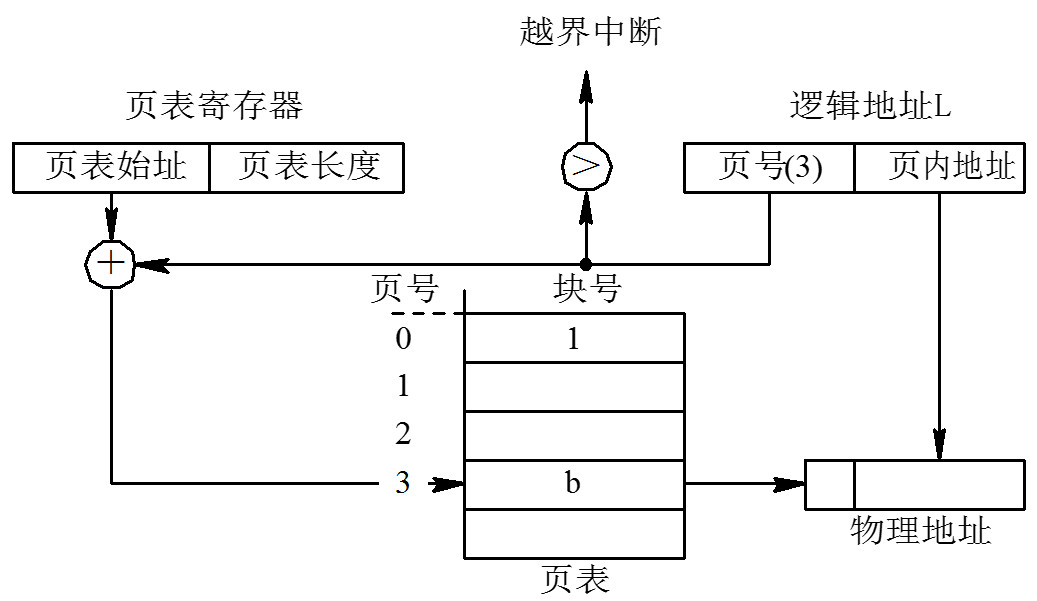
\includegraphics[width=0.9\textwidth]{figure/mem_page_dzbh.jpg}
  \end{center}
\end{frame}


\begin{frame}[fragile]{2 具有快表的地址变换机构 }
  \begin{easylist} 
    & 不具快表,则需两次访问内存。
    && (1)访页表
    && (2)得到绝对地址内容
    & 有快表,速度提高。
    & 快表贵,不能太多。
  \end{easylist}
\end{frame}


\begin{frame}[fragile]{快表}
  \begin{center}
    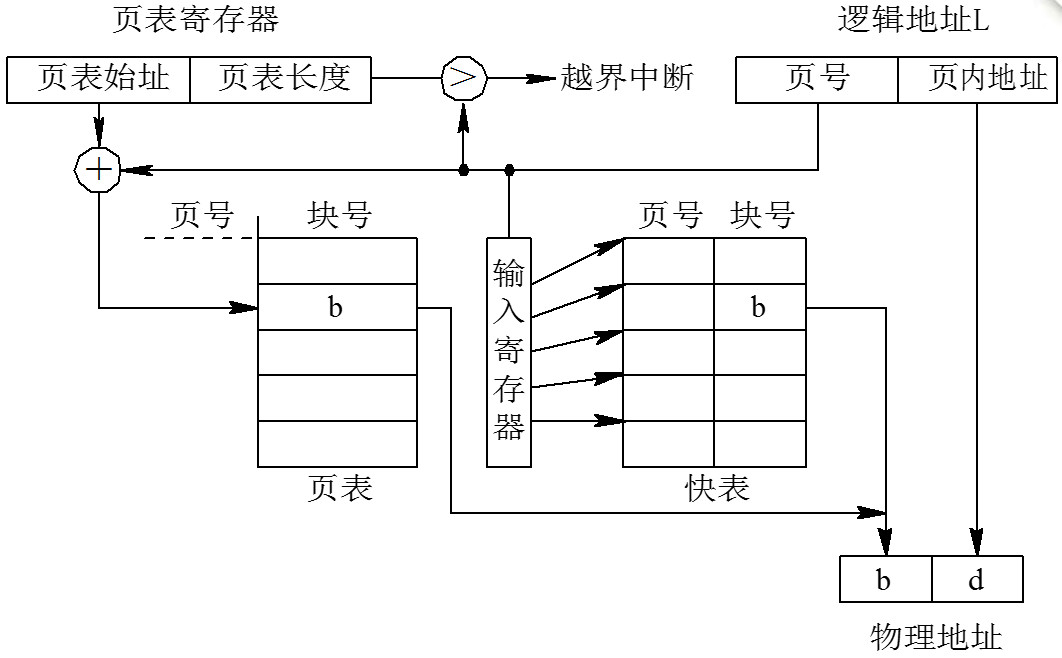
\includegraphics[width=0.9\textwidth]{figure/mem_page_cache.jpg}
  \end{center}
\end{frame}

\begin{frame}[fragile]{命中率}
  \begin{easylist} 
  & 命中率是指页号在快表中被查找到的百分比,记为$p$。则有效访问时间:
  && 访问快表的时间$\times p$ + 从内存中访问时间$\times (1-p)$
  \end{easylist}
\end{frame}


\begin{frame}[fragile]{练习}
  \begin{easylist} 
    & 有一页式系统,其页表存放在主存中:
    && 如果对主存的一次存取需要$1.5\mu s$,试问实现一次页面访问的存取时间是多少?
    && 如果系统加有快表,平均命中率为85\%,当页表项在快表中时,其查找时间忽略为0, 试问此时的存取时间是多少?
  \end{easylist}
\end{frame}

\begin{frame}[fragile]{Answer}
  \begin{easylist} 
   & 答:若页表存放在主存中,则要实现一次页面访问需两次访问主存:一次是访问页表,确定所存取页面的物理地址(称为定位)。第二次才根据该地址存取页面数据。
&& 页表在主存的存取访问时间
   $$=1.5 \times 2=3(\mu s)$$
&& 增加快表后的存取访问时间\\
  $$ =0.85 \times 1.5+(1-0.85) \times 2 \times 1.5=1.725(\mu s)$$
  \end{easylist}
\end{frame}


\begin{frame}[fragile]{练习}
  \begin{easylist} 
   & 在页式存储管理方法中,假定一页的大小为$1KB$,若一条指令在作业中的逻辑页号为
   2,页内偏移为200,该逻辑页对应的物理块的块号为7,则以四位十六进制表示的该指令
   的逻辑地址为(~~~~)H,物理地址为(~~~~)H。  \pause
   && 逻辑地址
   $$=P \times 1K+d=2×1024+200=(2248)_{10}$$
   $$ =(100011001000)_2=(08C8)_{16}$$  
   && 物理地址
   $$=f \times 1K+d=7×1024+200=(7368)_{10}$$
   $$ =(1110011001000)_2=(1CC8)_{16}$$
  \end{easylist}
\end{frame}


\begin{frame}[fragile]{4.3.3 两级和多级页表}
  \begin{easylist} 
  & 现代的大多数计算机系统,都支持非常大的逻辑地址空间($2^{32} \sim 2^{64}$)。在这样的环境下,
  页表就变得非常大,要占用相当大的内存空间。
  & 例子:
  && 对于一个具有32位逻辑地址空间的分页系统,规定页面大小为4KB即$2^{12}$B,则在
  每个进程页表中的页表项可达(~~~~)个。 
  && 每个页表项占用一个字节, 则每个进程仅其页表要占用的内存空间为(~~~~),该地址
  空间要求是(连续?|离散?)的。 \pause
  &&& 1M($\dfrac{2^{32}}{2^{12}}$)
  &&& 1M, 连续
   \end{easylist}
\end{frame}


\begin{frame}[fragile]{4.3.3 两级和多级页表}
  \begin{easylist} 
    & 解决办法:
    && 采用离散分配方式来解决难以找到一块连续的大内存空间的问题
    && 只将当前需要的部分页表项调入内存,其余的页表项仍驻留在磁盘上,需要时再调入
  \end{easylist}
\end{frame}


\begin{frame}[fragile]{1 两级页表(Two-Level Page Table)}
  \begin{easylist} 
   & 逻辑地址结构
  \end{easylist}
  \begin{center}
    \begin{tikzpicture}[]
      \coordinate (start) at (0,0);
      \draw[] node[minimum width=3cm, right=0 of start] (t1) {外层页号} node[right=0 of t1, minimum width=3cm] (t2){外层页内地址} node[right=0 of t2, minimum width=3.6cm] (t3){页内地址};
      \draw[yshift=-0.3cm, <->,blue,thick] (0,0)--(3,0);
      \draw[yshift=-0.3cm, <->,blue,thick] (3,0)--(6,0);
      \draw[yshift=-0.3cm, <->,blue,thick] (6,0)--(9.6,0);
      \draw[yshift=-1cm,thick] (0,0)--(9.6,0);
      \draw[thick] (0,-1)--(0,0.5) (3,-1)--(3,0.5) (6,-1)--(6,0.5) (9.6,-1)--(9.6,0.5);
      \draw[] node at(0,-1.5) {31} node at(2.75,-1.5) {22}  node at(3.25,-1.5) {21}
      node at(5.75,-1.5) {12}  node at(6.25,-1.5) {11}  node at(9.5,-1.5) {0};
    \end{tikzpicture}
  \end{center}
\end{frame}



\begin{frame}[fragile]{两级页表结构}
  \begin{center}
    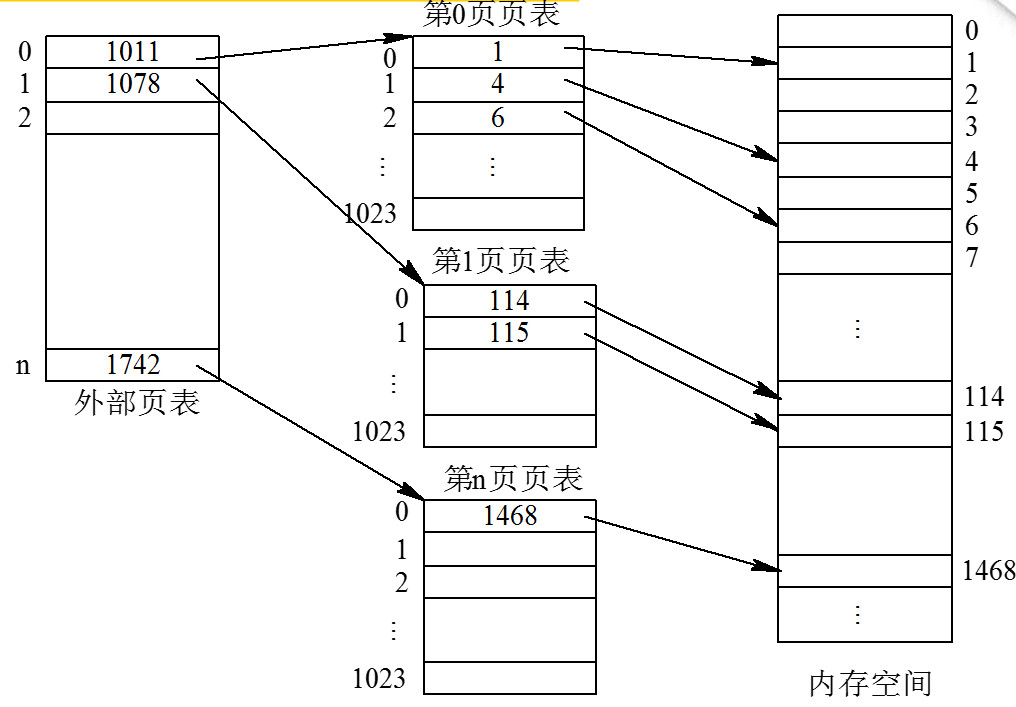
\includegraphics[width=0.9\textwidth]{figure/mem_page_ljyb.jpg}
  \end{center}
\end{frame}



\begin{frame}[fragile]{具有两级页表的地址变换机构}
  \begin{center}
    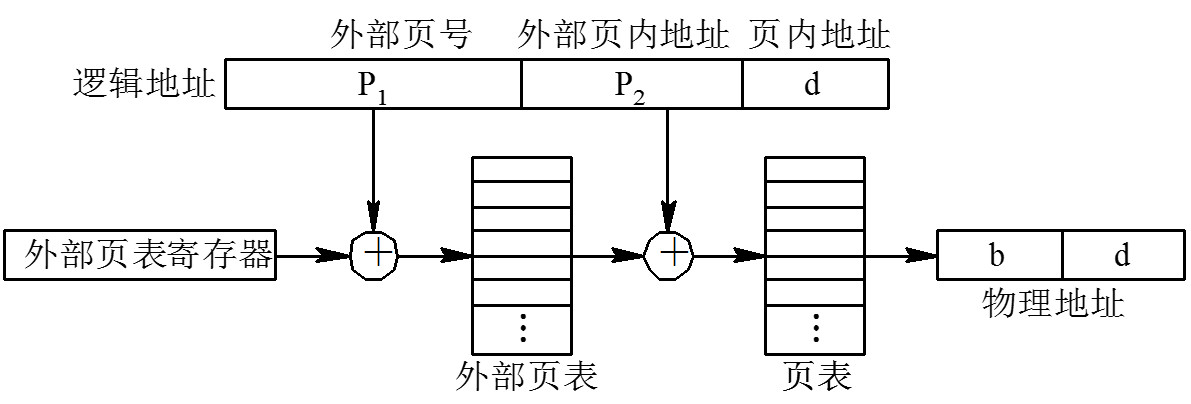
\includegraphics[width=0.9\textwidth]{figure/mem_page_ljyb2.jpg}
  \end{center}
\end{frame}


\begin{frame}[fragile]{2 多级页表}
  \begin{easylist} 
   & 对于32位的机器,采用两级页表结构是合适的;
   & 对于64位的机器,如果页面大小仍采用4KB即$2^{12}$B,即使按照两级页表划分,第
   二及页表的大小依然非常巨大
   && 引入多级页表
  \end{easylist}
\end{frame}

\begin{frame}[fragile]{NEXT}
  ~
\end{frame}


\subsection{4.4 基本分段式存储管理方式}
\begin{frame}[fragile]{4.4 基本分段式存储管理方式}
  \begin{easylist} 
    & 引入分页存储管理方式,主要是为了提高内存的利用率。而引入分段存储管理方式,主
    要是为了满足用户在编程和使用上多方面的要求。
    & 内容
    \begin{enumerate}
    \item 分段存储管理方式的引入
    \item 分段系统的基本原理
    \item 信息共享
    \item 段页式存储管理方式
    \end{enumerate}
  \end{easylist}
\end{frame}


\begin{frame}[fragile]{4.4.1分段存储管理方式的引入 }
  \begin{easylist} 
    & 引入分段存储管理方式,主要是为了满足用户和程序员的下述一系列需要:
    && 1) 方便编程
    && 2) 信息共享 
    && 3) 信息保护 
    && 4) 动态增长 
    && 5) 动态链接 
  \end{easylist}
\end{frame}



\begin{frame}[fragile]{4.4.2 分段系统的基本原理}
  \begin{easylist} 
    & 按程序自身的逻辑关系把作业的地址空间划分为若干个程序段,每个程序段都有一个
    段名,且有一个段号。段号从0开始,每一段也从0开始编址,段内地址是连续的。

  \end{easylist}
\end{frame}

\begin{frame}[fragile]{1. 分段的地址结构}
  \begin{easylist} 
  & 分段地址中的地址结构(二维的):\vspace{0.5cm}
  \begin{center}
    \begin{tikzpicture}[c/.style={draw,thick, minimum width=3cm, minimum height=0.8cm}]
      \draw[] node[c] (a) {段号} 
      node[c, right=0 of a] (b) {段内地址}
      node at (-1.5,-0.7) {31}
      node at (1.25,-0.7) {16} node at (1.75,-0.7) {15} node at (4.5,-0.7) {0} ;
    \end{tikzpicture}
  \end{center}
  & 分段方式已得到许多编译程序的支持,编译程序能自动地根据源程序的情况而产生若干
  个段。如Pascal、Fortran 
  \end{easylist}
\end{frame}

\begin{frame}[fragile]{2. 段表}
  \begin{easylist} 
  & 进程中每个分段分配一个连续的内存空间(分区),各个段可以离散地存放在内存中不
  同的分区。因此系统给每个进程建立一张映射表,简称“{\em 段表}”。{\em 段表是用于实现从逻辑段到物理内存分区的映射}。
  \end{easylist}
\end{frame}


\begin{frame}[fragile]{图:利用段表实现地址映射}
  \begin{center}
    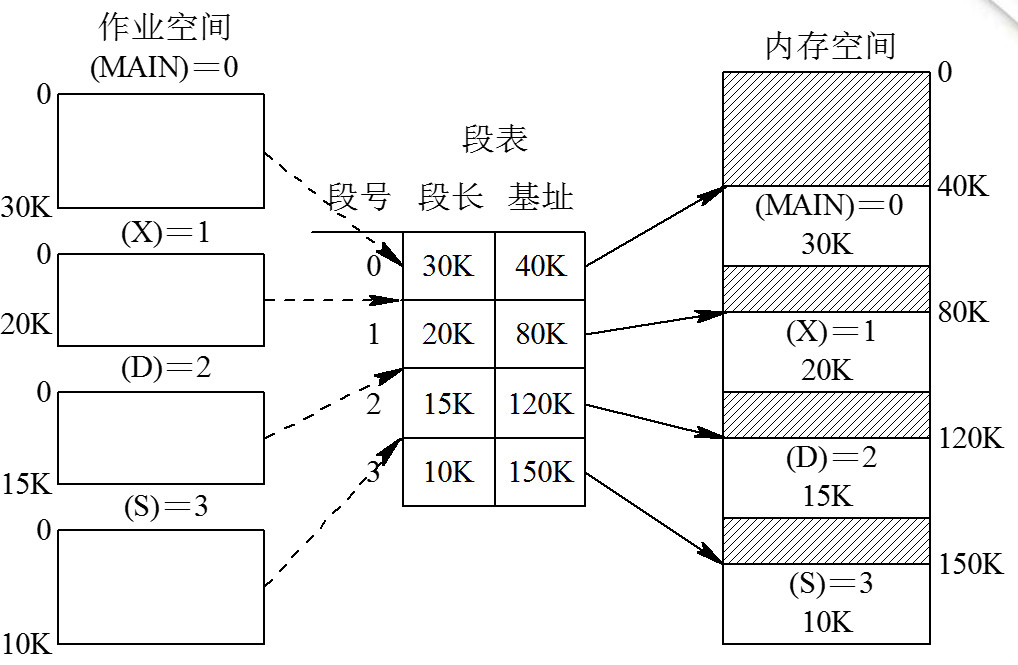
\includegraphics[width=0.8\textwidth]{figure/mem_seg1.jpg}
  \end{center}
\end{frame}

\begin{frame}[fragile]{3. 地址变换机构}
  \begin{center}
    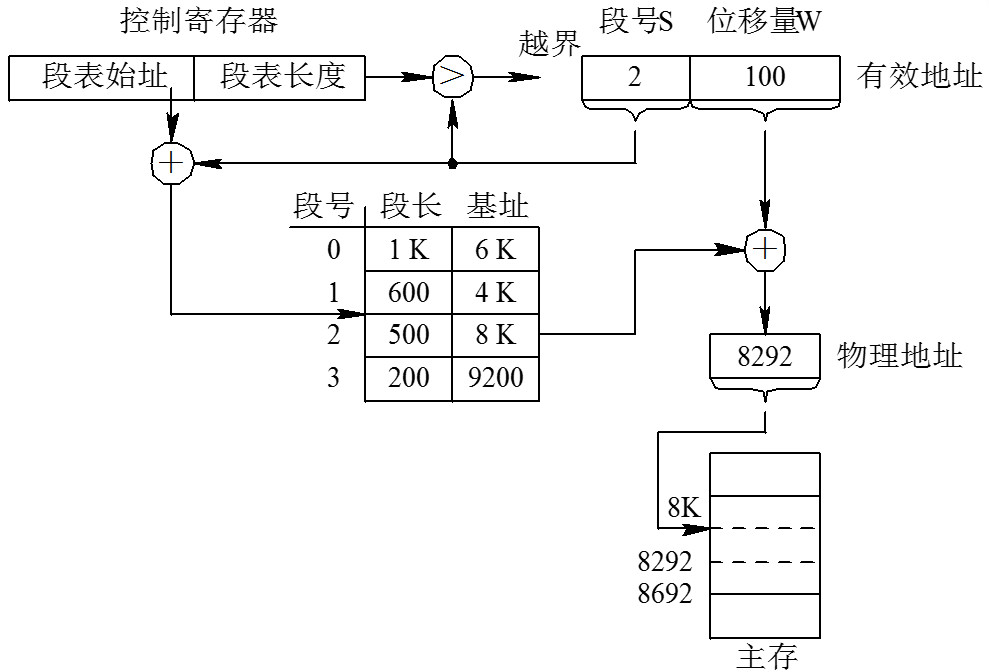
\includegraphics[width=0.8\textwidth]{figure/mem_seg2.jpg}
  \end{center}
\end{frame}

\begin{frame}[fragile]{问题}
  \begin{easylist} 
    & 要访问一个数据,需两次访问内存。同样也可以增设一个联想存储器(快表)。一般
    情况下段比页大,因而段表项的数目比页表项的数目少,其所需的联想存储器也比较小。
  \end{easylist}
\end{frame}

\begin{frame}[fragile]{4. 分页和分段的主要区别}
  \begin{easylist} 
    & [1] 页是信息的物理单位,分页是为实现离散分配方式,以消减内存的外零头, 提高
    内存的利用率。或者说, 分页仅仅是由于系统管理的需要而不是用户的需要。段则是信息
    的逻辑单位,它含有一组其意义相对完整的信息。 分段的目的是为了能更好地满足用户的
    需要。 
    & [2] 页的大小固定且由系统决定,由系统把逻辑地址划分为页号和页内地址两部分,是
    由机器硬件实现的,因而在系统中只能有一种大小的页面;而段的长度却不固定, 决定于
    用户所编写的程序,通常由编译程序在对源程序进行编译时,根据信息的性质来划分。
    & [3] 分页的作业地址空间是一维的,即单一的线性地址空间,程序员只需利用一个记忆
    符,即可表示一个地址; 而分段的作业地址空间则是二维的,程序员在标识一个地址时,
    既需给出段名,又需给出段内地址。
  \end{easylist}
\end{frame}



\begin{frame}[fragile]{4.4.3 信息共享}
  \begin{center}
    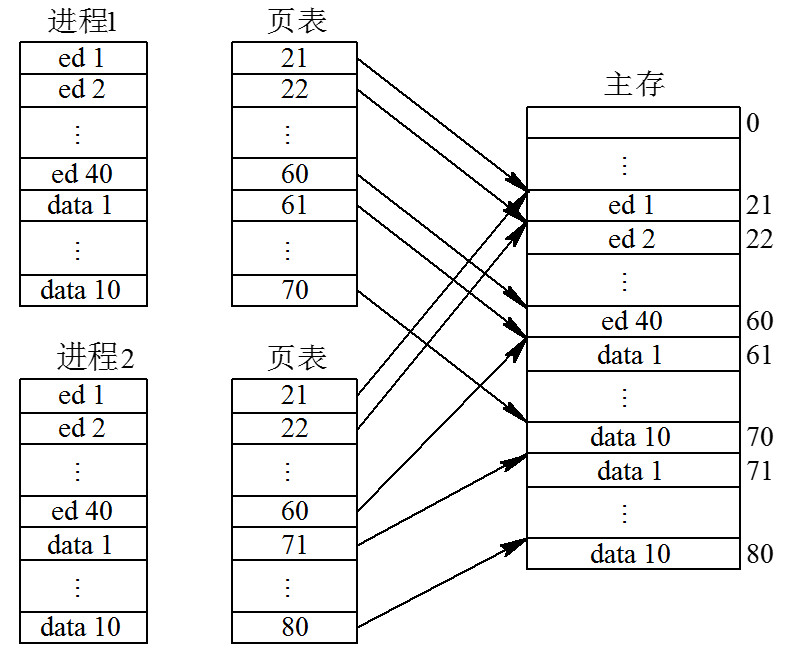
\includegraphics[width=0.7\textwidth]{figure/mem_seg3.jpg}
  \end{center}
\end{frame}


\begin{frame}[fragile]{分段系统中共享editor的示意图}
  分页系统中共享editor的示意图:
  \begin{center}
    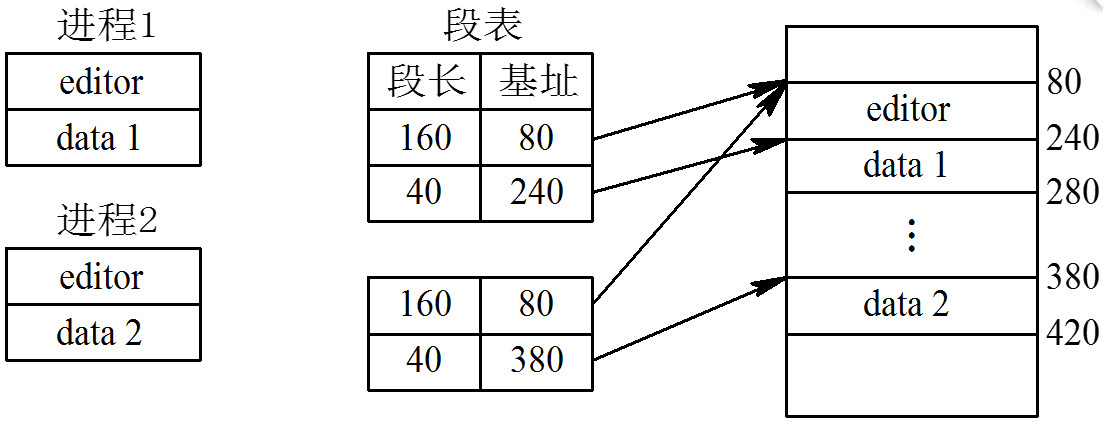
\includegraphics[width=0.8\textwidth]{figure/mem_seg4.jpg}
  \end{center}
\end{frame}


\begin{frame}[fragile]{可重入代码}
  \begin{easylist} 
    & 可重入代码又称为“纯代码”,是一种允许被多个进程同时访问的代码。
    && 为保证各个进程所执行的代码完全相同,绝对不允许可重入代码在执行中有任何改变。
    && 实际采用{\em 配备局部数据区},把执行中改变的部分拷贝到该数据区,程序执行
    只改变该进程私有的数据区,不改变共享的代码。
  \end{easylist}
\end{frame}

\begin{frame}[fragile]{4.4.4 段页式存储管理方式}
  \begin{easylist} 
    & 1 基本原理
    && 将用户程序划分若干个段,然后再把每个段分成若干页,并为每一段赋一个段名
  \end{easylist}
\end{frame}


\begin{frame}[fragile]{图: 作业地址空间和地址结构}
   \begin{center}
    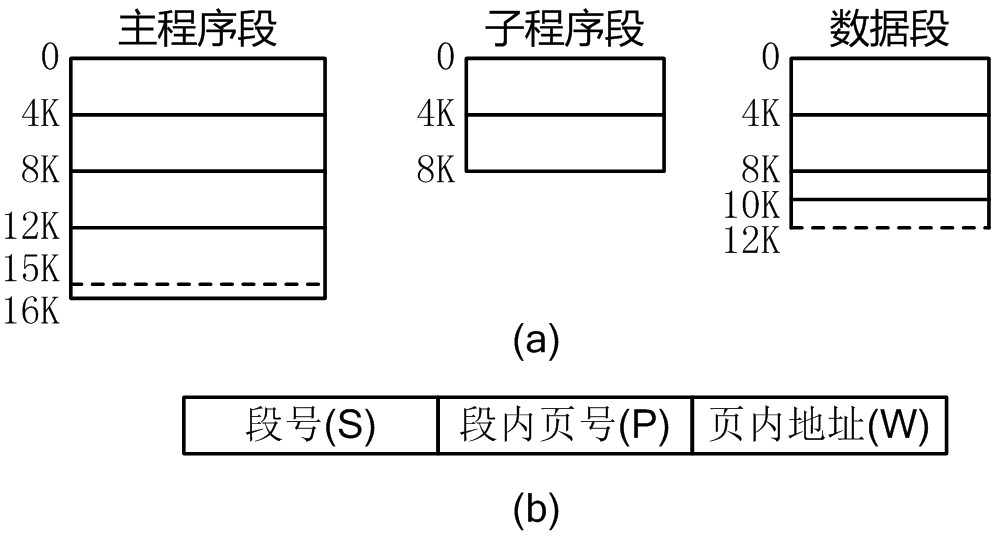
\includegraphics[width=0.8\textwidth]{figure/mem_seg5.jpg}
  \end{center}
\end{frame}


\begin{frame}[fragile]{图: 利用段表和页表实现地址映射}
 \begin{center}
    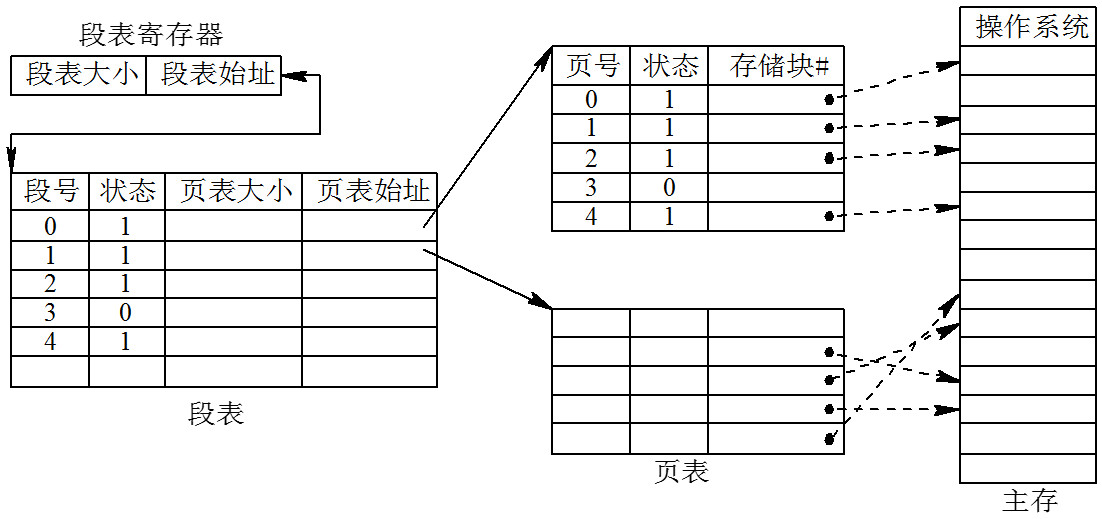
\includegraphics[width=1.0\textwidth]{figure/mem_seg6.jpg}
  \end{center}  
\end{frame}


\begin{frame}[fragile]{2 地址变换过程}
   \begin{center}
    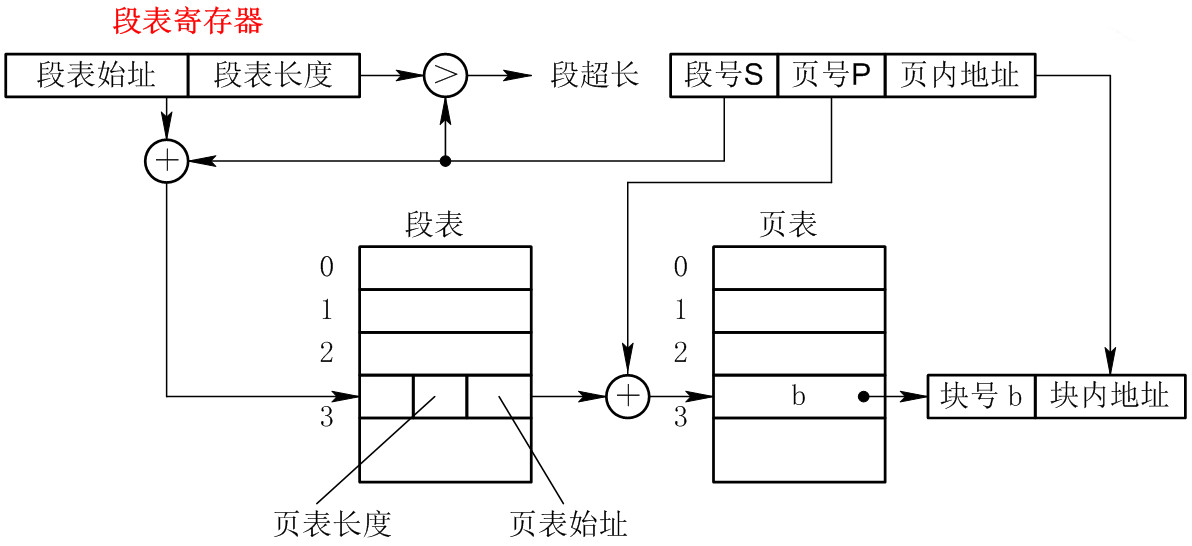
\includegraphics[width=1.0\textwidth]{figure/mem_seg7.jpg}
  \end{center}  
\end{frame}


\begin{frame}[fragile]{问题}
  \begin{easylist} 
  & 为获取一条指令或数据,需访问内存几次? \pause
  && 3次
  & 解决方法:
  && 要访问一个数据,需三次访问内存。同样也可以增设一个联想存储器(快表),存放段号和页号,访问时同时用段号和页号去检索高速缓存。
  \end{easylist}
\end{frame}

\begin{frame}[fragile]{问题}
  \begin{easylist} 
    & 连续分配方式和基本分页、分段方式的特点:要求作业全部装入内存后才能运行
    && (1) 有的作业很大,其所要求的内存空间超过了内存总容量,作业不能全部被装入
    内存,导致该作业无法运行。
    && (2) 有大量作业要求运行,但是由于内存容量不足以容纳所有这些作业,只能将少
    数的作业装入内存让它们先运行,而将其它大量的作业留在外存上等待。
    & 该怎么解决该问题?
  \end{easylist}
\end{frame}


\subsection{4.5 虚拟存储器的基本概念}
\begin{frame}[fragile]{4.5 虚拟存储器的基本概念}
  \begin{easylist} 
    & 4.5.1 虚拟存储器的引入
    & 4.5.2 虚拟存储器的实现方法
    & 4.5.3 虚拟存储器的特征
  \end{easylist}
\end{frame}

\begin{frame}[fragile]{4.5.1 虚拟存储器的引入}
  \begin{easylist} 
    & 1 常规存储器管理方式的特征
    && (1)一次性
    && (2) 驻留性
    \pause
    && 这两个特性使许多在运行中不用或暂时不用的程序/数据占据了大量的内存空间,使
    得一些需要运行的作业无法装入内存。
    && 这两个特性是否必须呢?
    &&& 程序执行的局部性
  \end{easylist}
\end{frame}

\begin{frame}[fragile]{2 局部性原理 — C++程序示例}
  \begin{center}
    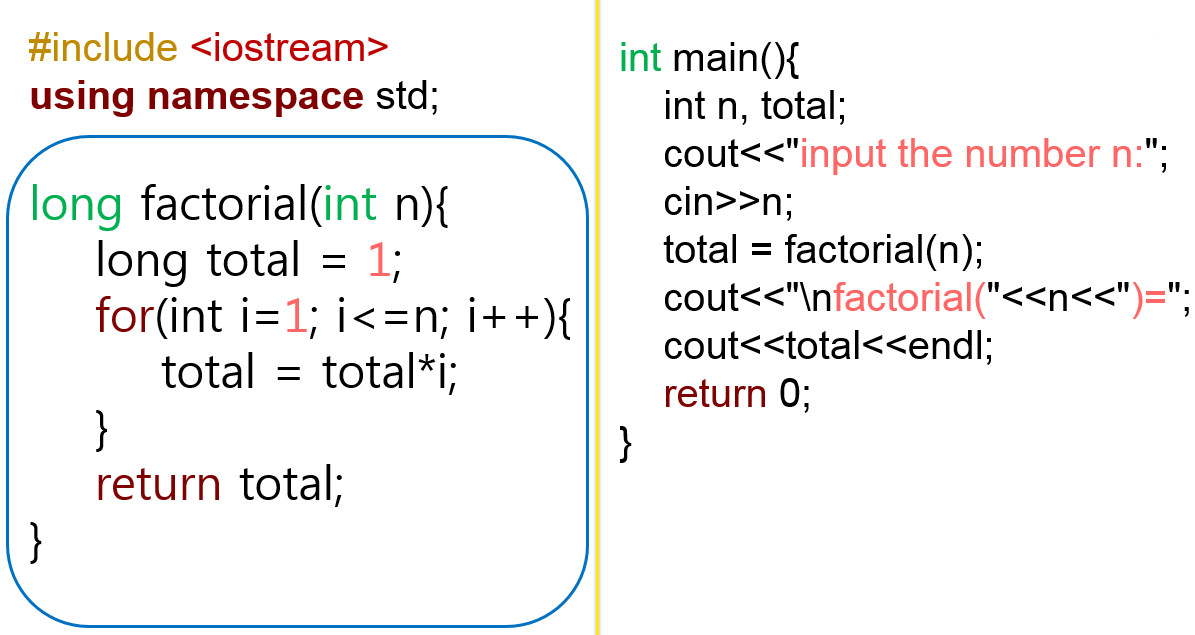
\includegraphics[width=1.0\textwidth]{figure/mem_virtual1.jpg}
  \end{center}
\end{frame}

\begin{frame}[fragile]{2 局部性原理}
  \begin{easylist} 
    & 早在1968年,Denning.P就曾指出: 
    && (1)程序执行时,除了少部分的转移和过程调用指令外,在大多数情况下仍是顺序执
    行的。
    && (2)过程调用将会使程序的执行轨迹由一部分区域转至另一部分区域,但经研究看出,
    过程调用的深度在大多数情况下都不超过5。
    && (3)程序中存在许多循环结构,这些虽然只由少数指令构成,但是它们将多次执行。
    && (4)程序中还包括许多对数据结构的处理,如对数组进行操作,它们往往都局限于很
    小的范围内。 
  \end{easylist}
\end{frame}

\begin{frame}[fragile]{局部性原理的表现方面}
  \begin{easylist} 
    & (1)时间局部性。
    && 如果程序中的某条指令一旦执行,则不久以后该指令可能再次执行;如果某数据被
    访问过, 则不久以后该数据可能再次被访问。产生时间局限性的典型原因,是由于在
    程序中存在着大量的循环操作。
    & (2)空间局部性。
    && 一旦程序访问了某个存储单元,在不久之后,其附近的存储单元也将被访问,即程
    序在一段时间内所访问的地址,可能集中在一定的范围之内,其典型情况便是程序的顺
    序执行
  \end{easylist}
\end{frame}

\begin{frame}[fragile]{3 虚拟存储器的定义}
  \begin{easylist} 
    & 虚拟存储器是指具有请求调入功能和置换功能,能从逻辑上对内存容量加以扩充的一
    种存储器系统。
    && 虚拟存储器的逻辑容量由内存容量和外存容量之和所决定,其运行速度接近于内存
    速度,而每比特的成本却又接近于外存。
    && 虚拟存储技术是一种性能非常优越的存储器管理技术,被广泛地应用于大、中、小
    型机器和微型机中。 
  \end{easylist}
\end{frame}

\begin{frame}[fragile]{4.5.2 虚拟存储器的实现方法}
  \begin{easylist} 
    & 1 分页请求系统 (以页面为单位)
    && (1)硬件支持
    &&& ①请求分页的页表机制,它是在纯分页的页表机制上增加若干项而形成的,作为请求分页的数据结构;
    &&& ②缺页中断机构,即每当用户程序要访问的页面尚未调入内存时便产生一缺页中断,以请求OS将所缺的页调入内存;
    &&& ③地址变换机构,它同样是在纯分页地址变换机构的基础上发展形成的。
    && (2)实现请求分页的软件(调页算法和置换算法)
  \end{easylist}
\end{frame}

\begin{frame}[fragile]{4.5.2 虚拟存储器的实现方法}
  \begin{easylist} 
    & 2 请求分段系统 (以段为单位)
    && (1)硬件支持
    &&& ①请求分段的段表机制,它是在纯分段的段表机制上增加若干项形成;
    &&& ②缺段中断机构,当访问尚未调入内存的分段时产生缺段中断,请求OS将所缺段调入;
    &&& ③地址变换机构。
    && (2)实现请求分段的软件(请求调段和段的置换)
  \end{easylist}
\end{frame}

\begin{frame}[fragile]{4.5.3 虚拟存储器的三个特征}
  \begin{easylist} 
    & 多次性
    && 多次性是指一个作业被分多次调入内存。多次性是虚拟存储器最重要的特征。
    & 对换性
    && 对换性是指允许在作业运行过程中换进、换出。换进和换出能够有效提高内存利用
    率。
    & 虚拟性
    && 虚拟性是指能够从逻辑上扩充内存容量,使用户所看到的内存容量远远大于实际容
    量。虚拟性是以多次性和对换性为基础的。
  \end{easylist}
\end{frame}

\begin{frame}[fragile]{Windows的虚拟内存设置}
  \begin{easylist} 
    & DEMO
  \end{easylist}
\end{frame}


\subsection{4.6 请求分页存储管理方式}
\begin{frame}[fragile]{4.6 请求分页存储管理方式}
  \begin{easylist} 
    & 建立在基本分页基础上,支持虚拟存储器功能,增加了请求调页和页面置换功能。
    && 每次调入和换出的基本单位都是长度固定的页面。
    && 比请求分段简单,是目前最常用的一种实现虚拟存储器的方式。
    \pause
    & 内容
    && 4.6.1 请求分页中的硬件支持
    && 4.6.2 内存分配策略和分配算法
    && 4.6.3 调页策略
  \end{easylist}
\end{frame}

\begin{frame}[fragile]{4.6.1 请求分页中的硬件支持}
  \begin{easylist} 
    & 1 页表机制
    & 2 缺页中断机构
    & 3 地址变换机构
  \end{easylist}
\end{frame}

\begin{frame}[fragile]{1 页表机制}
  \begin{center}
    \begin{tikzpicture}[c/.style={draw,thick, minimum width=1.5cm, minimum height=0.8cm}]
      \draw[] node[c] (a) {页号} 
      node[c, right=0 of a] (b) {物理块号}
      node[c, right=0 of b] (c) {状态位P}
      node[c, right=0 of c] (d) {访问字段A}
      node[c, right=0 of d] (e) {修改位M}
      node[c, right=0 of e] (f) {外存地址};

      \draw[draw,purple, dotted,-Latex, thick] node[c,below left=2 of c, xshift=1cm, rounded corners,fill=green!10] (g) {是否已经调入内存} (g.north)-- (c.south);

      \draw[draw, -Latex, dotted,thick, red] node[c,below left=4 of d, xshift=3cm, rounded corners,fill=green!10, align=center] (h) {被访问次数或多长时间未被访问,\\ 供选择换出页面时参考} (h.north)-- (d.south);

      \draw[draw, -Latex, dotted,thick, blue] node[c,below=2 of e,xshift=-0.5cm, rounded corners,fill=green!10] (f) {是否被修改过} (f.north)-- (e.south);
    \end{tikzpicture}
  \end{center}
\end{frame}

\begin{frame}[fragile]{2 缺页中断机构}
  \begin{easylist} 
    & 与一般中断的区别
    && 在指令执行期间产生和处理中断信号
    && 在一条指令执行期间,可能产生多次缺页中断
  \end{easylist}
\end{frame}

\begin{frame}[fragile]{图: 涉及6次缺页中断的指令}
  \begin{center}
    \begin{tikzpicture}[c/.style={draw,thick, minimum width=3cm, minimum height=0.8cm},
      c2/.style={draw,thick, minimum width=2cm, minimum height=0.5cm, red}]
      \draw[] node[c] (1) {} node[left=0.2 of 1] {1} 
      node[c, above=0 of 1] (2) {} node[left=0.2 of 2] {2}
      node[c, above=0 of 2] (3) {} node[left=0.2 of 3] {3}
      node[c, above=0 of 3] (4) {} node[left=0.2 of 4] {4}
      node[c, above=0 of 4] (5) {} node[left=0.2 of 5] {5}
      node[c, above=0 of 5] (6) {} node[left=0.2 of 6] {6} 
      node[above left=0 of 6] {页面};

      \draw[] node[c2, above=0 of 1]{copy $A$} node[c2, below=0 of 2]{to~~ $B$};
      \draw[] node[c2, above=0 of 3]{$A$ ...} node[c2, below=0 of 4]{$A$ ...};
      \draw[] node[c2, above=0 of 5]{$B$ ...} node[c2, below=0 of 6]{$B$ ...};
    \end{tikzpicture}
  \end{center}
\end{frame}

\begin{frame}[fragile]{3 地址变换机构}
  \begin{center}
    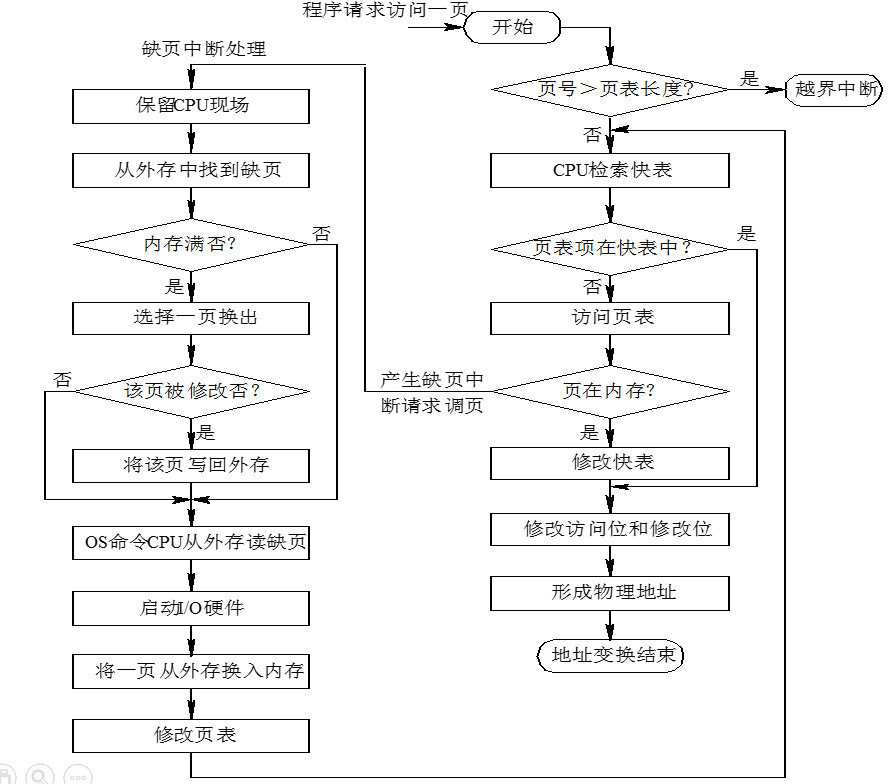
\includegraphics[width=0.8\textwidth]{figure/mem_virtual2.jpg}
  \end{center}
\end{frame}

\begin{frame}[fragile]{4.6.2 内存分配策略和分配算法}
  \begin{easylist} 
    & 1 最小物理块数的确定 
    && 最小物理块数是指能保证进程正常运行所需的最小物理块数。当系统为进程分配的
    物理块数少于此值时,进程将无法运行。
    && 最少物理块数与计算机硬件结构有关,取决于指令的格式、 功能和寻址方式。
    && 对于某些简单的机器,若是单地址指令且采用直接寻址方式,则所需的最少物理块
    数为2。
    其中,一块是用于存放指令的页面,另一块则是用于存放数据的页面。
    && 如果该机器允许间接寻址时,则至少要求有三个物理块。对于某些功能较强的机器,
    其指令长度可能是两个或多于两个字节,因而其指令本身有可能跨两个页面,且源地址
    和目标地址所涉及的区域也都可能跨两个页面。
  \end{easylist}
\end{frame}


\begin{frame}[fragile]{2 物理块的分配策略}
  \begin{easylist} 
    & 在请求分页系统中,可采取两种内存分配策略,即固定和可变分配策略。在进行置换
    时,也可采取两种策略,即全局置换和局部置换。于是可组合出以下三种适用的策略。
    && 1) 固定分配局部置换
    && 2) 可变分配全局置换 
    && 3) 可变分配局部置换
  \end{easylist}
\end{frame}

\begin{frame}[fragile]{固定分配局部置换}
  \begin{easylist} 
    & 为每个进程分配一定数目的物理块,在整个运行期间都不再改变。
    & 换出时,只能从该进程在内存的n个页面中选出一页换出,然后再调入一页,保证分
    配给该进程的内存空间不变。
    && 缺点:分配多少个物理块难以确定。
    &&& 太少,会频繁缺页,降低吞吐量;
    &&& 太多,则内存中驻留的进程数目减少,造成资源闲置。
  \end{easylist}
\end{frame}

\begin{frame}[fragile]{可变分配全局置换}
  \begin{easylist} 
    & 先为系统中的每个进程分配一定数目的物理块,OS自身也保持一个空闲物理块队列。
    缺页时,由系统从空闲物理块队列中,取出一个物理块分配给该进程。
    & 当空闲物理块用完后,OS从内存中选择任一进程的物理块调出。
  \end{easylist}
\end{frame}

\begin{frame}[fragile]{可变分配局部置换}
  \begin{easylist} 
    & 缺页时,从该进程在内存的页面中选择一页换出。(局部置换)
    & 如果频繁换页,则系统为该进程分配若干附加的物理块,直到缺页率减少到适当程度
    为止。(可变分配:增加)
    & 如缺页率特别低,则适当减少分配给该进程的物理块数。 (可变分配:减少)
  \end{easylist}
\end{frame}


\begin{frame}[fragile, allowframebreaks]{3 固定分配策略的分配算法}
  \begin{easylist} 
    & (1) 平均分配算法
    && 这是将系统中所有可供分配的物理块,平均分配给各个进程。
    && 例如,当系统中有100个物理块,有5个进程在运行时,每个进程可分得20个物理块。
    这种方式貌似公平,但实际上是不公平的,因为它未考虑到各进程本身的大小。如有一
    个进程其大小为200页,只分配给它20个块,这样,它必然会有很高的缺页率;而另一
    个进程只有10页,却有10个物理块闲置未用。
  \end{easylist}
  \newpage
  \begin{easylist} 
    & (2) 按比例分配算法
    && 这是根据进程的大小按比例分配物理块的算法。如果系统中共有$n$个进程,每个进程
    的页面数为$S_i$,则系统中各进程页面数的总和为:
    $$S=\sum_{i=1}^n S_i$$
    && 又假定系统中可用的物理块总数为$m$,则每个进程所能分到的物理块数为$b_i$,将
    有:
    $$b_i=\dfrac{S_i}{S} \cdot m$$
    &&& $b_i$应该取整,它必须大于最小物理块数。 
  \end{easylist}

  \newpage
  \begin{easylist}
    & (3) 考虑优先权的分配算法
    && 在实际应用中,为了照顾到重要的、紧迫的作业能尽快地完成,应为它分配较多的
    内存空间。
    && 通常采取的方法是把内存中可供分配的所有物理块分成两部分:
    &&& 一部分按比例地分配给各进程;
    &&& 另一部分则根据各进程的优先权,适当地增加其相应份额后,分配给各进程。在有
    的系统中,如重要的实时控制系统,则可能是完全按优先权来为各进程分配其物理块的。
  \end{easylist}
\end{frame}

\begin{frame}[fragile, allowframebreaks]{4.6.3 调页策略}
  \begin{easylist} 
    & 1 何时调入页面
    && 预调页策略
    &&& 将预计在不久之后便会访问的页面预先调入内存
    && 请求调页策略
    &&& 访问页不在内存时,立即提出请求,由OS将其调入内存。
    &&& 易于实现
    &&& 每次调入一页,开销较大
  \end{easylist}

  \newpage
  \begin{easylist}
    & 2 从何处调入页面
    && 在请求分页系统中的外存分为两部分:用于存放文件的文件区和用于存放对换页面
    的对换区。
    && 由于对换区是采用连续分配方式,而文件区是采用离散分配方式,故对换区的磁盘
    I/O速度比文件区的高。这样,每当发生缺页请求时,系统应从何处将缺页调入内存,
    可分成如下三种情况:
    \newpage
    &&& (1)系统拥有足够的对换区空间,这时可以全部从对换区调入所需页面,以提高调
    页速度。为此,在进程运行前,便须将与该进程有关的文件,从文件区拷贝到对换区。
    
    \newpage
    &&& (2)系统缺少足够的对换区空间,这时凡是不会被修改的文件,都直接从文件区调
    入;而当换出这些页面时,由于它们未被修改而不必再将它们换出,以后再调入时,仍
    从文件区直接调入。但对于那些可能被修改的部分,在将它们换出时,便须调到对换区,
    以后需要时,再从对换区调入。

    \newpage
    &&& (3)UNIX方式。由于与进程有关的文件都放在文件区,故凡是未运行过的页面,都
    应从文件区调入。而对于曾经运行过但又被换出的页面,由于是被放在对换区,因此在
    下次调入时,应从对换区调入。由于UNIX系统允许页面共享,因此, 某进程所请求的
    页面有可能已被其它进程调入内存,此时也就无须再从对换区调入。
  \end{easylist}

  \newpage
  \begin{easylist}
    & 3 页面调入过程
    && 页面未在内存时,便向CPU发出缺页中断,中断处理程序首先保留CPU环境,分析中
    断原因后, 转入缺页中断处理程序。
    && 该程序通过查找页表,得到该页在外存的物理块后, 如果此时内存能容纳新页,则
    启动磁盘I/O将所缺之页调入内存,然后修改页表。
    && 如果内存已满,则须先按照某种置换算法从内存中选出一页准备换出;如果该页未
    被修改过,就不必再写回磁盘;但如果已被修改,则必须将它写回磁盘,然后再把所缺
    的页调入内存,并修改页表中的相应表项,置其存在位为“1”,并写入快表。在缺页调
    入内存后,利用修改后的页表,去形成所要访问数据的物理地址,再去访问内存数据。
  \end{easylist}
\end{frame}


\begin{frame}[fragile]{~}
 ~
\end{frame}


\subsection{4.7 页面置换算法}
\begin{frame}[fragile]{4.7 页面置换算法}
  \begin{easylist} 
    & 页面置换算法是选择换出页面的算法。置换算法的好坏,将直接影响到系统的性能。
  \end{easylist}
\end{frame}


\begin{frame}[fragile]{4.7.1 最佳置换算法和先进先出置换算法}
  \begin{easylist} 
    & 1、最佳(Optimal)置换算法
    && 最佳置换算法是由Belady于1966年提出的一种理论上的算法。
    && 其所选择的被淘汰页面,将是以后永不使用的,或许是在最长(未来)时间内不再被
    访问的页面。
    && 采用最佳置换算法,通常可保证获得最低的缺页率。
  \end{easylist}
\end{frame}

\begin{frame}[fragile]{例}
  \begin{easylist} 
    & 假定系统为某进程分配了三个物理块, 并考虑有以下的页面号引用串:
    && 7,0,1,2,0,3,0,4,2,3,0,3,2,1,2,0,1,7,0,1
    && 进程运行时,先将7,0,1三个页面装入内存。以后,当进程要访问页面2时,将会
    产生缺页中断。此时OS根据最佳置换算法,将选择页面7予以淘汰。
  \end{easylist}
  \tiny
  \begin{center}
    \begin{tabular}{| l | c | c | c | c | c | c | c | c | c | c | c | c |c | c |c |c | c | c | c | c |}
      \hline
      \rowcolor{yellow!10}
      ~   & 7 & 0 & 1 & 2 & 0 & 3 & 0 & 4 & 2 & 3 & 0 & 3 & 2 & 1 & 2 & 0 & 1 & 7 & 0 & 1 \\
      \hline
      块1 & 7 & 7 & 7 & 2 & ~ & 2 & ~ & 2 & ~ & ~ & 2 & ~ & ~ & 2 & ~ & ~ & ~ & 7 & ~ & ~ \\ 
      块2 & ~ & 0 & 0 & 0 & ~ & 0 & ~ & 4 & ~ & ~ & 0 & ~ & ~ & 0 & ~ & ~ & ~ & 0 & ~ & ~ \\ 
      块3 & ~ & ~ & 1 & 1 & ~ & 3 & ~ & 3 & ~ & ~ & 3 & ~ & ~ & 1 & ~ & ~ & ~ & 1 & ~ & ~ \\ 
      \hline
    \end{tabular}
  \end{center}
\end{frame}

\begin{frame}[fragile]{2 先进先出(FIFO)页面置换算法}
  \tiny
  \begin{center}
    \begin{tabular}{| l | c | c | c | c | c | c | c | c | c | c | c | c |c | c |c |c | c | c | c | c |}
      \hline
      \rowcolor{yellow!10}
      ~   & 7 & 0 & 1 & 2 & 0 & 3 & 0 & 4 & 2 & 3 & 0 & 3 & 2 & 1 & 2 & 0 & 1 & 7 & 0 & 1 \\
      \hline
      块1 & 7 & 7 & 7 & 2 & ~ & 2 & 2 & 4 & 4 & 4 & 0 & ~ & ~ & 0 & 0 & ~ & ~ & 7 & 7 & 7 \\ 
      块2 & ~ & 0 & 0 & 0 & ~ & 3 & 3 & 3 & 2 & 2 & 2 & ~ & ~ & 1 & 1 & ~ & ~ & 1 & 0 & 0 \\ 
      块3 & ~ & ~ & 1 & 1 & ~ & 1 & 0 & 0 & 0 & 3 & 3 & ~ & ~ & 3 & 2 & ~ & ~ & 2 & 2 & 1 \\ 
      \hline
    \end{tabular}
  \end{center}
\end{frame}

\begin{frame}[fragile]{4.7.2 最近最久未使用(LRU)置换算法 }
  \begin{easylist} 
    & 1、LRU (Least Recently Used)置换算法的描述 
  \end{easylist}

  \tiny
  \begin{center}
    \begin{tabular}{| l | c | c | c | c | c | c | c | c | c | c | c | c |c | c |c |c | c | c | c | c |}
      \hline
      \rowcolor{yellow!10}
      ~   & 7 & 0 & 1 & 2 & 0 & 3 & 0 & 4 & 2 & 3 & 0 & 3 & 2 & 1 & 2 & 0 & 1 & 7 & 0 & 1 \\
      \hline
      块1 & 7 & 7 & 7 & 2 & ~ & 2 & ~ & 4 & 4 & 4 & 0 & ~ & ~ & 1 & ~ & 1 & ~ & 1 & ~ & ~ \\ 
      块2 & ~ & 0 & 0 & 0 & ~ & 0 & ~ & 0 & 0 & 3 & 3 & ~ & ~ & 3 & ~ & 0 & ~ & 0 & ~ & ~ \\ 
      块3 & ~ & ~ & 1 & 1 & ~ & 3 & ~ & 3 & 2 & 2 & 2 & ~ & ~ & 2 & ~ & 2 & ~ & 7 & ~ & ~ \\ 
      \hline
    \end{tabular}
  \end{center}
\end{frame}

\begin{frame}[fragile]{2、LRU算法的硬件支持}
  \begin{easylist} 
    & 1)寄存器
    && 为了记录某进程在内存中各页的使用情况,须为每个在内存中的页面配置一个移位
    寄存器,可表示为 
    $$R=R_{n-1}R_{n-2}R_{n-3} \cdots R_2 R_1 R_0$$
  \end{easylist}
\end{frame}

\begin{frame}[fragile]{图:某进程具有8个页面时的LRU访问情况}
  \begin{center}
    \begin{tabular}{| l | c | c | c | c | c | c |c |c | c | c | c | c |}
      \hline
      \rowcolor{yellow!10}
      ~   & 4 & 3 & 2 & 1 & 4 & 3 & 5 & 4 & 3 & 2 & 1 & 5  \\
      \hline
      块1 & 4 & 4 & 4 & 1 & 1 & 1 & 5 & ~ & ~ & 2 & 2 & 2 \\ 
      块2 & ~ & 3 & 3 & 3 & 4 & 4 & 4 & ~ & ~ & 4 & 1 & 1 \\ 
      块3 & ~ & ~ & 2 & 2 & 2 & 3 & 3 & ~ & ~ & 3 & 3 & 5 \\ 
      \hline
    \end{tabular}
  \end{center}
\end{frame}

\begin{frame}[fragile]{2) 栈}
  \begin{easylist} 
    & 用栈保存当前使用页面时栈的变化情况
  \end{easylist}

  \begin{center}
    \newcolumntype{g}{>{\columncolor{black!2}}c}
    \begin{tabular}{| g | c | c | c | c | c | c | c | c |}
      \hline
      \rowcolor{yellow!10}
      分页  & $R_7$ & $R_6$ & $R_5$ & $R_4$ & $R_3$ & $R_2$ & $R_1$ & $R_0$ \\
      \hline
      1 & 0 & 1 & 0 & 1 & 0 & 0 & 1 & 0 \\
      2 & 1 & 0 & 1 & 0 & 1 & 1 & 0 & 0 \\
      3 & 0 & 0 & 0 & 0 & 0 & 1 & 0 & 0 \\
      4 & 0 & 1 & 1 & 0 & 1 & 0 & 1 & 1 \\
      5 & 1 & 1 & 0 & 1 & 1 & 1 & 1 & 0 \\
      6 & 0 & 0 & 1 & 0 & 1 & 0 & 1 & 1 \\
      7 & 0 & 0 & 0 & 0 & 0 & 1 & 1 & 1 \\
      8 & 0 & 1 & 1 & 0 & 1 & 1 & 0 & 1 \\
      \hline
    \end{tabular}
  \end{center}
\end{frame}

\begin{frame}[fragile]{4.7.3 Clock置换算法}
  \begin{easylist} 
    & 1、简单的Clock置换算法 
  \end{easylist}
  \begin{center}
    \begin{tikzpicture}[b/.style={draw,minimum width=2cm, minimum height=0.6cm},
      b4/.style={draw,minimum width=1cm, minimum height=0.6cm, fill=yellow!15}]
      \draw node[b, fill=green!10](h1){块号} node[b,right=0 of h1, fill=green!10](h2){ 页号 }  node[b,right=0 of h2, fill=green!10](h3){访问位}  node[b4,right=0 of h3, fill=green!10](h4){指针} ;
      \draw node[b, below=0 of h1](b01){0} node[b,right=0 of b01](b02){ }  node[b,right=0 of b02](b03){ }  node[b4,right=0 of b03](b04){ } ;
      \draw node[b, below=0 of b01](b11){1} node[b,right=0 of b11](b12){ }  node[b,right=0 of b12](b13){ }  node[b4,right=0 of b13](b14){ } ;
      \draw node[b, below=0 of b11](b21){2} node[b,right=0 of b21](b22){4 }  node[b,right=0 of b22](b23){0 }  node[b4,right=0 of b23](b24){ } ;
      \draw node[b, below=0 of b21](b31){3} node[b,right=0 of b31](b32){ }  node[b,right=0 of b32](b33){ }  node[b4,right=0 of b33](b34){ } ;
      \draw node[b, below=0 of b31](b41){4} node[b,right=0 of b41](b42){2 }  node[b,right=0 of b42](b43){1 }  node[b4,right=0 of b43](b44){ } ;
      \draw node[b, below=0 of b41](b51){5} node[b,right=0 of b51](b52){ }  node[b,right=0 of b52](b53){ }  node[b4,right=0 of b53](b54){ } ;
      \draw node[b, below=0 of b51](b61){6} node[b,right=0 of b61](b62){5 }  node[b,right=0 of b62](b63){ 0}  node[b4,right=0 of b63](b64){ } ;
      \draw node[b, below=0 of b61](b71){7} node[b,right=0 of b71](b72){ 1}  node[b,right=0 of b72](b73){1 }  node[b4,right=0 of b73](b74){ } ;

      \draw node[right=of b24, yshift=0.15cm](p){替换指针};
      \draw[-latex, thick] (p) -- +(-2.3,0);

      \draw[-latex, thick] (b24.345) --+(-0.3,0) -- ++(1,0) -- ++(0,-1) -- ++(-1.5,0);
      \draw[-latex, thick] (b44.345) --+(-0.3,0) -- ++(1,0) -- ++(0,-1) -- ++(-1.5,0);
      \draw[-latex, thick] (b64.345) --+(-0.3,0) -- ++(1,0) -- ++(0,-0.5) -- ++(-1.5,0);
    \end{tikzpicture}
  \end{center}
\end{frame}

\begin{frame}[fragile]{2 改进的Clock置换算法}
  \begin{easylist}
    & 由访问位A和修改位M可以组合成下面四种类型的页面:
    && 1类(A=0, M=0):表示该页最近既未被访问,又未被修改,是最佳淘汰页。
    && 2类(A=0, M=1):表示该页最近未被访问, 但已被修改,并不是很好的淘汰页。
    && 3类(A=1, M=0):最近已被访问,但未被修改,该页有可能再被访问。
    && 4类(A=1, M=1):最近已被访问且被修改, 该页可能再被访问。
  \end{easylist}
\end{frame}


\begin{frame}[fragile]{执行过程}
  \begin{easylist}
    & (1)从指针所指示的当前位置开始,扫描循环队列,寻找A=0且M=0的第一类页面,将
    所遇到的第一个页面作为所选中的淘汰页。在第一次扫描期间不改变访问位A。
    & (2)如果第一步失败,即查找一周后未遇到第一类页面,则开始第二轮扫描,寻找A=0
    且M=1的第二类页面,将所遇到的第一个这类页面作为淘汰页。在第二轮扫描期间,将
    所有扫描过的页面的访问位都置0。
    & (3)如果第二步也失败,亦即未找到第二类页面,则将指针返回到开始的位置,并将
    所有的访问位复0。然后重复第一步,如果仍失败,必要时再重复第二步,此时就一定
    能找到被淘汰的页。 
  \end{easylist}
\end{frame}

\begin{frame}[fragile]{4.7.4 其他置换算法}
  \begin{easylist}
    & 最少使用置换算法
    && (LFU:Least Frequently Used)
    & 页面缓冲算法
    && (PBA:Page Buffering Algorithm) 
  \end{easylist}
\end{frame}

\begin{frame}[fragile]{练习}
  \begin{easylist}
& 在一个请求分页存储管理系统中,一个作业的页面走向为4、3、2、1、4、3、5、4、3、2、1、5,当分配给该作业的物理块数分别为3、4时,试计算采用下述页面算法时的缺页次数(假设开始执行时主存中没有页面),并比较所得结果。
&& (1) 最佳置换法(OPT)
&& (2) 先进先出法(FIFO)
  \end{easylist}
\end{frame}

\begin{frame}[fragile]{解:OPT,物理块为3时}
  (1) 根据所给页面走向,使用最佳置换算法时,页面置换情况如下:
  
  \begin{center}
    \begin{tabular}{| l | c | c | c | c | c | c | c | c | c | c | c | c |}
      \hline
      \rowcolor{yellow!10}
      ~   & 4 & 3 & 2 & 1 & 4 & 3 & 5 & 4 & 3 & 2 & 1 & 5 \\
      \hline
      块1 & 4 & 4 & 4 & 4 & ~ & ~ & 4 & ~ & ~ & 2 & 2 & ~ \\ 
      块2 & ~ & 3 & 3 & 3 & ~ & ~ & 3 & ~ & ~ & 3 & 1 & ~ \\ 
      块3 & ~ & ~ & 2 & 1 & ~ & ~ & 5 & ~ & ~ & 5 & 5 & ~ \\
      \hline
    \end{tabular}
  \end{center}

  因此,缺页次数为7;
\end{frame}

\begin{frame}[fragile]{解:OPT,物理块为4时}
  \begin{center}
    \begin{tabular}{| l | c | c | c | c | c | c | c | c | c | c | c | c |}
      \hline
      \rowcolor{yellow!10}
      ~   & 4 & 3 & 2 & 1 & 4 & 3 & 5 & 4 & 3 & 2 & 1 & 5 \\
      \hline
      块1 & 4 & 4 & 4 & 4 & ~ & ~ & 4 & ~ & ~ & ~ & 1 & ~ \\ 
      块2 & ~ & 3 & 3 & 3 & ~ & ~ & 3 & ~ & ~ & ~ & 3 & ~ \\ 
      块3 & ~ & ~ & 2 & 2 & ~ & ~ & 2 & ~ & ~ & ~ & 2 & ~ \\
      块4 & ~ & ~ & ~ & 1 & ~ & ~ & 5 & ~ & ~ & ~ & 5 & ~ \\
      \hline
    \end{tabular}
  \end{center}

  \begin{easylist}
    & 因此,缺页次数为6。
    & 由上述结果可以看出,增加分配给作业的内存块数可以降低缺页次数。
  \end{easylist}
\end{frame}

\begin{frame}[fragile]{解:FIFO,物理块为3时}
  (2) 根据所给页面走向,使用先进先出页面置换算法时,页面置换情况如下:
    % \includegraphics[width=0.9\textwidth]{figure/mem_replace8.jpg}

  \begin{center}
    \begin{tabular}{| l | c | c | c | c | c | c | c | c | c | c | c | c |}
      \hline
      \rowcolor{yellow!10}
      ~   & 4 & 3 & 2 & 1 & 4 & 3 & 5 & 4 & 3 & 2 & 1 & 5 \\
      \hline
      块1 & 4 & 4 & 4 & 1 & 1 & 1 & 5 & ~ & ~ & 5 & 5 & ~ \\ 
      块2 & ~ & 3 & 3 & 3 & 4 & 4 & 4 & ~ & ~ & 2 & 2 & ~ \\ 
      块3 & ~ & ~ & 2 & 2 & 2 & 3 & 3 & ~ & ~ & 3 & 1 & ~ \\
      \hline
    \end{tabular}
  \end{center}

  因此,缺页次数为9;
\end{frame}


\begin{frame}[fragile]{解:FIFO,物理块为4时}
  \begin{center}
    \begin{tabular}{| l | c | c | c | c | c | c | c | c | c | c | c | c |}
      \hline
      \rowcolor{yellow!10}
      ~   & 4 & 3 & 2 & 1 & 4 & 3 & 5 & 4 & 3 & 2 & 1 & 5 \\
      \hline
      块1 & 4 & 4 & 4 & 4 & ~ & ~ & 5 & 5 & 5 & 5 & 1 & 1 \\ 
      块2 & ~ & 3 & 3 & 3 & ~ & ~ & 3 & 4 & 4 & 4 & 4 & 5 \\ 
      块3 & ~ & ~ & 2 & 2 & ~ & ~ & 2 & 2 & 3 & 3 & 3 & 3 \\
      块4 & ~ & ~ & ~ & 1 & ~ & ~ & 1 & 1 & 1 & 2 & 2 & 2 \\
      \hline
    \end{tabular}
  \end{center}

  \begin{easylist}
    & 因此,缺页次数为10;
    & 由上述结果可以看出,对先进先出算法而言,增加分配给作业的内存块数反而出现缺页次数增加的异常现象。
  \end{easylist}
\end{frame}


\subsection{4.8 请求分段存储管理方式}
\begin{frame}[fragile]{4.8 请求分段存储管理方式}
  略...
\end{frame}


\begin{frame}[fragile]{练习}
  \begin{easylist} \easyitem
    & 简述逻辑地址和物理地址
    & 固定分区、可变分区和页式存储管理各有什么样的优缺点
    & 分页管理中为什么需要页表?简述其作用。
    & 简述利用请求分页实现虚拟存储器的基本原理
  \end{easylist}
\end{frame}

\begin{frame}[fragile]{实验}
  \begin{easylist}
    & 实现LRU算法和FIFO算法
    & 要求
    && 给出任意的输入流、计算缺页率。
    && 输入流长度、分配的物理块$B$的大小可定制。
    && 例如:
    &&& $B=5$, 逻辑页为0-9个数字的任意排序,输入流的长度为30。
    &&& 输入流:1 2 5 6 8 3 6 5 3 6 5 6 8 9 2 7 0 4 9 5 3 6 7 4 5 8 7 3 4 5
  \end{easylist}
\end{frame}

\begin{frame}
  \begin{center}
    \Huge END
  \end{center}
\end{frame}

%%% Local Variables:
%%% mode: latex
%%% TeX-master: "../os"
%%% End:

%\section{设备管理}

\begin{frame}[fragile]{CH5 设备管理}
  \begin{easylist} \easyitem
    & 5.0 引言
    & 5.1 I/O系统的硬件组成
    & 5.2 I/O控制方式
    & 5.3 缓冲管理
    & 5.4 设备分配
    & 5.5 设备处理
    & 5.6 磁盘存储器管理
  \end{easylist}
\end{frame}


\subsection{引言}
\begin{frame}[fragile]{问题}
  \begin{easylist}
    & 设备管理的主要目标是什么?
    & 对应的主要解决途径是什么?
  \end{easylist}
\end{frame}

\begin{frame}[fragile]{引言}
  \begin{easylist}
    & “设备”泛指计算机系统中的外部设备,即除主机以外的其他所有设备。在多道程序设
    计环境下,计算机系统允许多个用户作业同时在内存,它们的运行势必涉及到I/O设备。
    & 带来三个问题 \pause
    && 对于设备本身,如何有效利用的问题;
    && 对于设备和CPU,如何发挥并行工作能力的问题;
    && 对于设备和用户,有一个如何方便使用的问题。
  \end{easylist}
\end{frame}

\begin{frame}[fragile]{引言}
  \begin{easylist}
    & 设备无关性
    && 操作系统必须向设备发送命令,捕捉中断,并处理设备的各种错误,还应提供其他
    部分使用设备的简单接口,如有可能,这个接口对所有设备都相同,这就是所谓的“与
    设备无关性”。
    & 虚拟设备
    && 在众多的I/O设备中,并不是所有的设备都是可以共享使用的。也就是说,当一个作
    业使用某种设备时,另一个要使用的作业只能暂时等待,一直到对方使用完毕,它才能
    去使用,这影响了系统效率的发挥。在设备管理中,仍然可以借助于磁盘,把只能独享
    的设备变为共享,这就是所谓的“虚拟设备”
  \end{easylist}
\end{frame}

\begin{frame}[fragile]{引言:设备管理的功能}
  \begin{easylist}
    & 缓冲区管理
    & 设备分配
    & 设备处理
    & 虚拟设备
    & 设备独立性
  \end{easylist}
\end{frame}

\begin{frame}[fragile]{通用设备管理分层模型}
  \begin{easylist}
    & 现代操作系统都采用分层结构构建设备管理模型,一种常见的设备管理模型如图
  \end{easylist}
  \begin{center} 
    \scalebox{0.8}{
      \begin{tikzpicture}[c/.style={draw,thick, minimum width=3cm, minimum height=0.75cm}, a/.style={<->, very thick}]
        \draw[] node[c] (b1) {用户进程} 
        node[c, below=0.5 of b1] (b2) {设备硬件无关层}
        node[c, below=0.5 of b2] (b3) {设备硬件相关层}
        node[c, below=0.5 of b3] (b4) {设备硬件} ;
        \draw[a] (b1)--(b2);
        \draw[a] (b2)--(b3);
        \draw[a] (b3)--(b4);
        \scriptsize
        \draw[] node[align=center,shape=ellipse, dotted, draw, fill=gray!5, minimum height=1cm,inner sep=0.1cm, left=0.5 of b3] (tip1) {实现\\I/O缓冲区管理\\以及\\设备映射功能};
        \draw[] node[align=center,shape=ellipse, dotted, draw, fill=gray!5, minimum height=1cm,inner sep=0cm, right=0.5cm of b2] (tip2) {将设备硬件无关层与硬件设备隔离开来。\\ 从设备硬件无关层看,设备硬件相关层为\\其提供了一个相对简洁的I/O功能接口;\\该接口屏蔽了设备硬件复杂的操作细节。\\从设备硬件相关层内部看,\\该层主要实现了设备驱动功能
        };
        \draw[->] (tip1)--(b2.west);
        \draw[->] (tip2)--(b3.east);
      \end{tikzpicture}
    }
  \end{center}
\end{frame}


\subsection{5.1 I/O系统的硬件组成}
\begin{frame}[fragile]{5.1 I/O系统的硬件组成}
  \begin{easylist}
    & 5.1.1 IO设备
    & 5.1.2 设备控制器
    & 5.1.3 IO通道
    & 5.1.4 总线系统
  \end{easylist}
\end{frame}

\subsubsection{5.1.1 IO设备}
\begin{frame}[fragile]{5.1.1 IO设备}
  \begin{enumerate}
    \item IO设备的类型
    \item 设备与控制器之间的接口
  \end{enumerate}
\end{frame}

\begin{frame}[fragile, allowframebreaks]{I/O设备的类型}
  \begin{easylist}
    & (1)按速度分:
    && 低速设备:典型设备有键盘、 鼠标器、语音的输入和输出等设备
    && 中速设备:典型设备有行式打印机、激光打印机等
    && 高速设备:典型设备有磁带机、 磁盘机、 光盘机等
    & (2)按信息交换的单位分类
    && 块设备(Block Device):用于存储信息,属于有结构设备。典型的块设备是磁盘。
    磁盘设备的基本特征是其传输速率较高,另一特征是可寻址,即对它可随机地读/写任
    一块;此外,磁盘设备的I/O常采用DMA方式
    && 字符设备(Character Device):用于数据的输入和输出,属于无结构设备。典型字
    符设备如交互式终端、打印机等。基本特征是其传输速率较低,另一特征是不可寻址;
    此外,常采用中断驱动方式
    \newpage
    & (3)按设备的共享属性分:
    && 独占:如临界资源
    && 共享:磁盘
    && 虚拟:本身为独占,但将其虚拟为几个逻辑设备。
  \end{easylist}
\end{frame}

\begin{frame}[fragile]{设备与控制器之间的接口}
  \begin{easylist}
    & CPU $\leftrightarrow$ 控制器 $\leftrightarrow$ 设备
    & 传统的设备由机械部分和电子部分组成,电子部分在系统的控制下驱动机械部分运转,
    形成I/O操作。
    & 电子部分比机械部分速度快,为降低硬件成本,将电子部分从设备中分立出来作为一
    个独立的部件,即设备控制器。
    & 设备不直接与CPU通信,而是通过设备控制器通信。
  \end{easylist}
\end{frame}

\begin{frame}[fragile]{设备与设备控制器间的接口}
  \begin{center}
    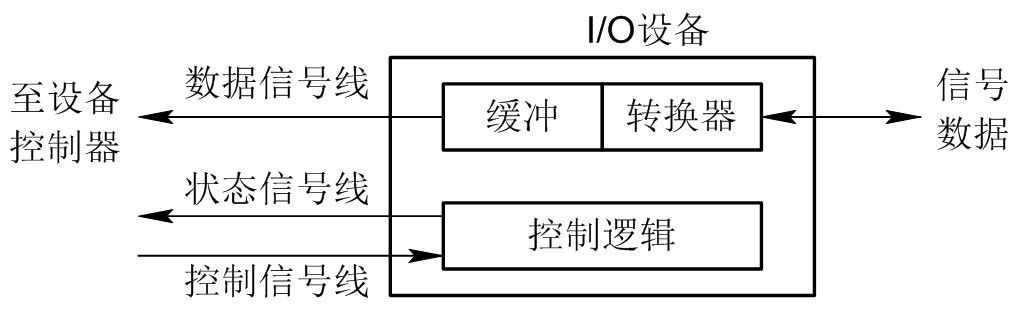
\includegraphics[width=0.9\textwidth]{figure/dev-interface.jpg}
  \end{center}
  \begin{easylist}
    & 数据信号线
    && 在设备与设备控制器之间传送数据信号
    & 状态信号线
    && 传送指示设备当前状态的信号
    & 控制信号线
    && 设备控制器向I/O设备发送控制信号用
  \end{easylist}
\end{frame}

\begin{frame}[fragile]{设备与控制器之间的接口传递的信号}
  \begin{enumerate}
    \item 数据信号:——双向,有缓存
    \item 控制信号:控制器发给设备;要求其完成相关操作
    \item 状态信号:设备发给控制器,后者“显示”;
  \end{enumerate}

  \begin{easylist}
    & IO设备控制的变化
    && 两级(CPU $\leftrightarrow$ IO设备)
    && 三级(CPU $\leftrightarrow$ 控制器  $\leftrightarrow$ IO设备)
    && 四级(CPU $\leftrightarrow$ IO通道 $\leftrightarrow$ 控制器  $\leftrightarrow$ IO设备)
  \end{easylist}
\end{frame}

\begin{frame}[fragile]{讨论:促使IO控制不断发展的推动因素}
  \pause
  \begin{easylist}
    & 减少CPU对IO的干预,充分利用CPU的处理能力
    & 缓和速度不匹配问题
    & 提高CPU和IO的并行程度,使CPU和IO尽可能忙碌。
  \end{easylist}
\end{frame}


\subsubsection{5.1.2 设备控制器}
\begin{frame}[fragile]{5.1.2 设备控制器}
  \begin{easylist}
    & 分类
    && 控制块设备的控制器
    && 控制字符设备的控制器
    & 设备控制器的基本功能
    & 设备控制器的组成
  \end{easylist}
\end{frame}

\begin{frame}[fragile]{设备控制器的基本功能}
  \begin{easylist}
    & 接收CPU命令,控制I/O设备工作,解放CPU.
    & 1.接收和识别命令。
    && 应有相应的Register来存放命令(“命令寄存器”)
    & 2.数据交换:\small{ CPU $\leftrightarrow$ 控制器的数据寄存器  $\leftrightarrow$ 设备}
    & 3.设备状态的了解和报告
    && 设备控制器中的“状态寄存器” 
    & 4.地址识别
    && CPU通过“地址”与设备通信,设备控制器应能识别它所控制的设备地址以及其各寄存
    器的地址。
    & 5.数据缓冲
    && 适配高速的CUP和内存与低速的外设之间的问题
    & 6.差错控制
    && 对由IO设备传来的数据进行差错检测
  \end{easylist}
\end{frame}

\begin{frame}[fragile]{设备控制器组成}
  \begin{easylist}
    & 设备控制器与处理机的接口
    && 实现CPU与控制器通信,共有三类信号线:数据线、地址线和控制线
    && 两类寄存器:数据寄存器、控制/状态寄存器
    & 设备控制器与设备的接口
    && 一个设备控制器连接一个或多个设备,每个接口中都存有数据、控制、状态三种类型的信号
    & I/O逻辑:在其控制下完成与CPU、设备的通信。
  \end{easylist}
\end{frame}

\begin{frame}[fragile]{设备控制器的组成示意图}
  \begin{center}
    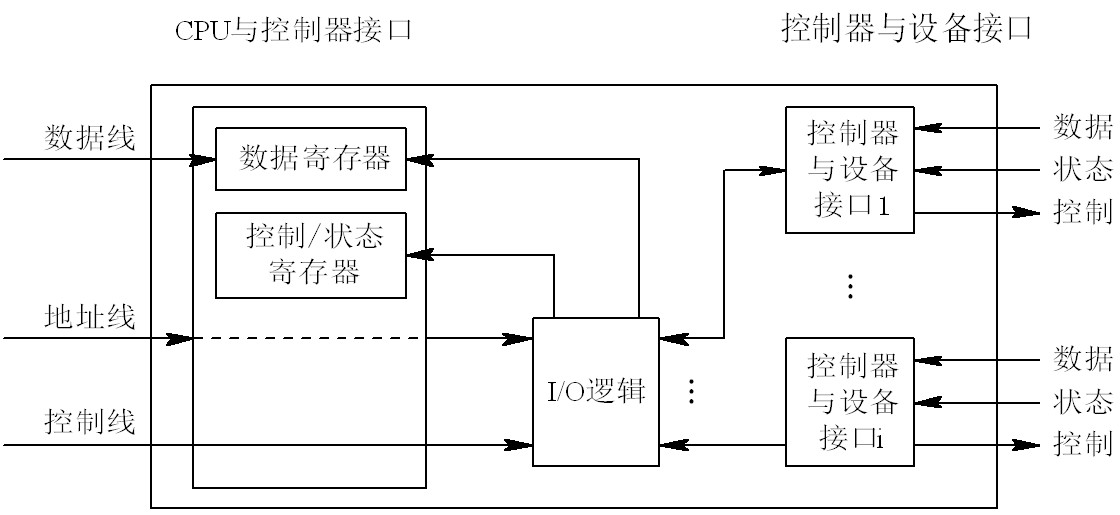
\includegraphics[width=0.9\textwidth]{figure/dev-controller.jpg}
  \end{center}
\end{frame}


\subsubsection{5.1.3 IO通道}
\begin{frame}[fragile]{5.1.3 IO通道}
  \begin{easylist}
    & 通道
    && 一种特殊的执行I/O指令的处理机,与CPU共享内存,可以有自己的总线。
    & 引入目的
    && 解脱CPU对I/O的组织、管理:建立独立的I/O操作,不仅使数据的传送能力独立于
    CPU,而且对有关对I/O操作的组织、管理及其结束处理也尽量独立,以保证CPU有更多
    的时间去进行数据处理。
    & CPU只需发送I/O命令给通道,通道通过调用内存中的相应通道程序完成任务。
    & I/O通道是一种特殊的处理机,具有执行I/O指令的能力,并通过执行通道(I/O)程序
    来控制I/O操作
  \end{easylist}
\end{frame}

\begin{frame}[fragile]{I/O通道与一般的处理机的区别}
  \begin{easylist}
    & 指令类型单一
    & 通道没有自己的内存,通道与CPU共享内存
    & 因为简单,所以价格便宜
  \end{easylist}
\end{frame}

\begin{frame}[fragile]{IO通道的类型}
  \begin{easylist}
    & 1.字节多路通道:
    && 各子通道以时间片轮转方式共享通道,适用于低、中速设备。
    & 2.数组选择通道:
    && 无子通道,仅一主通道,某时间由某设备独占,适于高速设备。
    && 但通道未共享,利用率低。
    & 3.数组多路通道:
    && 多子通道不是以时间片方式,而是“按需分配”,综合了前面2种通道类型的优点。
  \end{easylist}
\end{frame}

\begin{frame}[fragile]{I/O设备通道连接方式 }
  \begin{center}
    \includegraphics[width=0.9\textwidth]{figure/dev-channel.jpg}
  \end{center}
\end{frame}

\begin{frame}[fragile]{单通路通道“瓶颈”问题}
  \begin{center}
    \includegraphics[width=0.9\textwidth]{figure/dev-channel2.jpg}
  \end{center}
\end{frame}

\begin{frame}[fragile]{采用复联方式-多通路}
  \begin{center}
    \includegraphics[width=0.9\textwidth]{figure/dev-channel3.jpg}
  \end{center}
\end{frame}

\subsubsection{5.1.4 总线系统}
\begin{frame}[fragile]{5.1.4 总线系统}
  \begin{easylist}
    & 一、微机I/O系统
    \includegraphics[width=0.8\textwidth]{figure/dev-bus.jpg}

    && 处理机与I/O设备之间的基本连接都是通过总线实现的。即处理机连接在总线上,与
设备无关。设备则根据需要连接在相应的总线上,可多可少,结构和安装均十分灵活
    &&& 如:磁盘设备,打印设备; 缺点:总线瓶颈,CPU瓶颈。
    && ISA/EISA/Local BUS/VESA/PCI 

    & 二、主机I/O系统(四级结构)
    && 计算机—I/O通道—I/O控制器—设备
    && I/O通道相当于对总线的扩展,即多总线方式,且通道有一定的智能性,能与CPU并
行,解决其负担。
    \end{easylist}
\end{frame}


\subsection{5.2 I/O控制方式}
\begin{frame}[fragile]{5.2 I/O控制方式}
  \begin{easylist}
    & 四个发展阶段:
    && 程序I/O
    && 中断I/O
    && DMA控制
    && 通道控制。
    \vspace{1cm}
    & 趋势:提高并行度。
  \end{easylist}
\end{frame}

\subsubsection{5.2.1 程序I/O(忙—等待方式)}
\begin{frame}[fragile]{5.2.1 程序I/O(忙—等待方式)}
  \begin{columns}[onlytextwidth,T]
    \begin{column}{0.45\textwidth}
      \begin{itemize}
        \item 查询方式:CPU需花代价不断查询I/O状态
        \item CPU资源浪费极大。
        \item 例:99.9ms+0.1ms=100ms  
        \item 99.9在忙等
      \end{itemize}
    \end{column}
    \begin{column}{0.55\textwidth}
      \scalebox{0.6}{        
        \begin{tikzpicture}[c/.style={align=center, draw, minimum width=3cm}]
          \small
          \coordinate (top) at (0,0);
          \coordinate (ltop) at (-3,0);
          \draw node[c, below=0.5 of top] (b1) {向I/O控制器\\发读命令} node[right=0.5 of b1] {CPU $\rightarrow$ I/O}
          node[c, below=0.5 of b1] (b2) {读I/O控制器\\的状态}  node[right=0.5 of b2] {I/O $\rightarrow$ CPU}
          node[c, below=0.5 of b2, diamond, inner sep=-0.1cm] (b3) {检查\\状态?} node[right=of b3] (b3r) {出错}
          node[c, below=0.5 of b3] (b4) {从I/O控制器\\中读入字}  node[right=0.5 of b4] {I/O $\rightarrow$ CPU}
          node[c, below=0.5 of b4] (b5) {向存储器\\中写字}  node[right=0.5 of b5] {CPU $\rightarrow$ 内存}
          node[c, below=0.5 of b5, diamond, inner sep=-0.1cm] (b6) {传送\\完成?}
          node[below=0.5 of b6] (b7) {下条指令};

          \coordinate (mtop) at ($(b1)!.45!(b2)$);
          \coordinate (lmtop) at (mtop)[xshift=-2cm];

          \path[->] (b1) edge (b2) (b2) edge (b3) (b3) edge (b4) (b4) edge (b5) (b5) edge (b6) (b6) edge node[right]{完成} (b7) (b3) edge (b3r) (top) ++(0,0.3cm) edge (b1);

          \draw[->] (b3.west) -- ++(-1,0) |- ($(b1)!.45!(b2)$) node[align=center, left=0.5 of b2]{未\\就\\绪};
          \draw[->] (b6.west) -| (ltop) --(top) node[align=center, left=0.1 of b6, yshift=0.3cm]{未完};
        \end{tikzpicture}
      }
    \end{column}
  \end{columns}
\end{frame}


\subsubsection{5.2.2 中断I/O}
\begin{frame}[fragile]{5.2.2 中断I/O}
  \begin{columns}[onlytextwidth,T]
    \begin{column}{0.45\textwidth}
      \begin{itemize}
        \item 向I/O发命令$\rightarrow$返回$\rightarrow$执行其它任务。
        \item I/O中断产生$\rightarrow$CPU转相应中断处理程序。
        \item 如:读数据,读完后以中断方式通知CPU,CPU完成数据从I/O$\rightarrow$内存
        \item 以字(节)为单位进行干预
        \item CPU、设备并行工作
        \item 提高了系统的资源利用率和吞吐量
      \end{itemize}
    \end{column}
    \begin{column}{0.55\textwidth}
      \scalebox{0.6}{        
        \begin{tikzpicture}[c/.style={align=center, draw, minimum width=3cm}]
          \small
          \coordinate (top) at (0,0);
          \coordinate (ltop) at (-3,0);
          \draw node[c, below=0.5 of top] (b1) {向I/O控制器\\发读命令} node[right=0.5 of b1, yshift=0.3cm] {CPU $\rightarrow$ I/O} node[right=0.8 of b1, yshift=-0.3cm] (b1r2) {CPU做其他事情}
          node[c, below=0.5 of b1] (b2) {读I/O控制器\\的状态}  node[right=0.5 of b2,yshift=-0.3cm] {I/O $\rightarrow$ CPU} node[right=0.8 of b2,yshift=0.3cm] (b2r1) {中断} 
          node[c, below=0.5 of b2, diamond, inner sep=-0.1cm] (b3) {检查\\状态?} node[right=of b3] (b3r) {出错}
          node[c, below=0.5 of b3] (b4) {从I/O控制器\\中读入字}  node[right=0.5 of b4] {I/O $\rightarrow$ CPU}
          node[c, below=0.5 of b4] (b5) {向存储器\\中写字}  node[right=0.5 of b5] {CPU $\rightarrow$ 内存}
          node[c, below=0.5 of b5, diamond, inner sep=-0.1cm] (b6) {传送\\完成?}
          node[below=0.5 of b6] (b7) {下条指令};

          \draw[<-, dashed] (b1r2.west)--++(-0.7,0);
          \draw[->, dashed] (b2r1.west)--++(-0.7,0);
          \path[->] (b1) edge (b2) (b2) edge (b3) (b3) edge (b4) (b4) edge (b5) (b5) edge (b6) (b6) edge node[right]{完成} (b7) (b3) edge (b3r) (top) ++(0,0.3cm) edge (b1);

          \draw[->] (b6.west) -| (ltop) --(top) node[align=center, left=0.1 of b6, yshift=0.3cm]{未完};
        \end{tikzpicture}
      }
    \end{column}
  \end{columns}
\end{frame}


\subsubsection{5.2.3 DMA方式——用于块设备中}
\begin{frame}[fragile]{5.2.3 DMA方式——用于块设备中}
  \begin{easylist}
    & 一、DMA(Direct Memory Access)控制方式的引入
    && 中断I/O,CPU按字节干预,即每字节传送产生一次中断。
    && DMA:由DMA控制器直接控制总线传递数据块。DMA控制器完成从I/O——内存。
    & 特点:
    && ① 数据传输的基本单位是数据块,即在CPU与I/O设备之间,每次传送至少一个数据
    块;
    && ② 所传送数据从设备直接送入内存,或者相反;
    && ③ 仅在传送一个或多个数据块的开始和结束时,才需CPU干预,整块数据的传送由控
    制器控制完成。
    & 二、组成
    && 一组寄存器+控制逻辑。
    && CR(命令/状态);  DR(数据);  MAR(内存地址);  DC(计数)
  \end{easylist}
\end{frame}

\begin{frame}[fragile]{DMA控制器的组成图}
  \begin{center}
    \scalebox{0.7}{
      \begin{tikzpicture}[c/.style={align=center, draw, minimum width=1cm, minimum height=0.5cm}]
        \draw node[draw, minimum height=3.2cm, minimum width=2cm] (cpu) {} node[above=0.2 of cpu]{CPU}
        node[draw, minimum height=3.2cm, minimum width=2cm, right=0.5 of cpu] (mem) {} node[above=0.2 of mem]{内存}
        node[draw, minimum height=3.2cm, minimum width=6cm, right=0.5 of mem] (dma) {} node[above=0.2 of dma]{主机--控制器接口~~~控制器与块设备接口};

        \draw node[c, minimum height=1.6cm, minimum width=0.6cm, left=0.2 of mem.east, yshift=0.2cm] (mb){} node[left=0.1 of mb](count){count};
        \draw[] (mb.north)--++(-1,0)  (mb.south)--++(-1,0) ;
        \draw[<-] (mb.north) ++(-0.8,0) --++(0,-0.6);
        \draw[<-] (mb.south) ++(-0.8,0) --++(0,0.6);

        \draw node[c, right=1 of mem, yshift=1cm] (dr) {DR}  node[c, below=0.2 of dr] (mar) {MAR}   node[c, below=0.2 of mar] (dc) {DC}   node[c, below=0.2 of dc] (cr) {CR} 
        node[c, right=0.5 of dr, minimum height=2.6cm, yshift=-1.1cm](io) {I/O\\控\\制\\逻\\辑}
        node[c, right=0.5 of io, minimum height=1cm, minimum width=2cm, yshift=0.8cm] (block1) {} node[c, minimum height=1cm, minimum width=2cm, below=0.5 of block1]{};

        \draw[-latex] (mar.west) -- ($(mb.east) + (0,0.8)$);
        \draw[-latex] (dc.west)--(count.south);
        \draw[] (cpu.south) -- ++(0,-1) -| (mem) (mem.south) ++(0,-1) -| (dma);
        \path[-Latex] (cpu.south) ++(0.5,-0.5) edge node[above] {命令} ++(1.5,0);
        \draw node[below=0.3 of mem, xshift=2cm]{系统总线} node[below=0.2 of dma, xshift=2cm]{DMA控制器};
      \end{tikzpicture}
    }
  \end{center}
  \small
  \begin{easylist}
    && 数据寄存器DR: 用于暂存从设备到内存,或从内存到设备的数据
    && 内存地址寄存器MAR: 在输入时,它存放把数据从设备传送到内存的起始目标地址;
    在输出时,它存放由内存到设备的内存源地址
    && 数据计数器DC:  存放本次CPU要读或写的字(节)数
    && 命令/状态寄存器CR。用于接收从CPU发来的I/O命令或有关控制信息, 或设备的状
    态
  \end{easylist}
\end{frame}

\begin{frame}[fragile, plain]
  % \frametitle{DMA示意图}
  \begin{center}
    \includegraphics[width=0.9\textwidth]{figure/DMA.jpg}
  \end{center}
\end{frame}

\begin{frame}[fragile]{DMA工作过程}
  \begin{center}
    \includegraphics[width=0.75\textwidth]{figure/dev-dma2.jpg}
  \end{center}
\end{frame}

\begin{frame}[fragile]{讨论:中断驱动IO和DMA的区别}
  \begin{easylist}
    & 中断频率
    & 数据的传送方式
  \end{easylist}
\end{frame}

\subsubsection{5.2.4 I/O通道控制方式}
\begin{frame}[fragile]{5.2.4 I/O通道控制方式(1)}
  \begin{easylist}
    & I/O通道控制方式的引入
    && DMA方式:对许多离散块的读取仍需要多次中断。
    && 对一组数据块的读(或写)及有关的控制和管理为单位的干预
    && 实现CPU、通道和I/O设备三者的并行操作,从而更有效地提高整个系统的资源利用率
  \end{easylist}
\end{frame}

\begin{frame}[fragile]{5-2-4  I/O通道控制方式(2)}
  \begin{easylist}
    & 通道方式:CPU只需给出
    && (1)通道程序首址。
    && (2)要访问I/O设备后,通道程序就可完成一组块操作 
  \end{easylist}
\end{frame}

\begin{frame}[fragile]{通道程序的指令信息}
  \begin{easylist}
    & (1)操作码:指令所执行的操作
    & (2)内存地址:字符送入内存(读操作)或从内存取出(写操作)时的内存首址
    & (3)计数:要读写的字节数
    & (4)通道程序结束位P:P=1表示最后一条指令
    & (5)记录结束标志R,R=0,表示本指令和下一条指令处理的数据同属于一个记录。
  \end{easylist}
\end{frame}

\begin{frame}[fragile]{通道程序}
  \begin{easylist}
    & (1) 操作码	(2) 内存地址
    & (3) 计数 	(4) 通道程序结束位P 
    & (5) 记录结束标志R 
  \end{easylist}
  \begin{center}
    \begin{tabular}{|c|c|c|c|c|}
      \hline
      操作 & P & R & 计数 & 内存地址 \\ \hline
      WRITE & 0 & 0 & 80 & 813 \\ \hline
      WRITE & 0 & 0 & 140 & 1034 \\ \hline
      WRITE & 0 & 1 & 60 & 5830 \\ \hline
      WRITE & 0 & 1 & 300 & 2000 \\ \hline
      WRITE & 0 & 0 & 250 & 1850 \\ \hline
      WRITE & 1 & 1 & 250 & 720 \\ \hline
    \end{tabular}
  \end{center}
\end{frame}


\subsection{5.3 缓冲管理}
\begin{frame}[fragile]{5.3 缓冲管理}
~
\end{frame}

\subsubsection{5.3.1 缓冲的引入}
\begin{frame}[fragile]{5.3.1 缓冲的引入}
  \begin{easylist}
    & 1.缓和CPU和I/O设备间速度不匹配的矛盾。
    && 如:计算——打印buffer——打印
    & 2.减少对CPU的中断频率
    && 如:buffer越大,“buffer满”信号发生频率越低。
    & 3.提高CPU和I/O并行性 
  \end{easylist}
\end{frame}

\begin{frame}[fragile]{例子}
  \begin{center}
    \includegraphics[width=0.7\textwidth]{figure/dev-buffer-demo.jpg}
  \end{center}
  \begin{easylist}
    & (a) CPU中断频率:9.6Kb/s; CPU响应时间:约100us
    & (b) CPU中断频率:1.2Kb/s; CPU响应时间:约800us
    & (c) CPU中断频率:0.6Kb/s; CPU响应时间:约1600us
  \end{easylist}
\end{frame}

\subsubsection{5.3.2 单缓冲和双缓冲}
\begin{frame}[fragile]{5.3.2 单缓冲和双缓冲(1)}
  \begin{easylist}
    & 单缓冲(Single Buffer)
    & 系统对数据的处理时间:Max(C,T)+M
  \end{easylist}
  \begin{center}
    \includegraphics[width=0.9\textwidth]{figure/dev-buffer-single.jpg}
  \end{center}
\end{frame}

\begin{frame}[fragile]{5.3.2 单缓冲和双缓冲(2)}
  \begin{easylist}
    & 双缓冲(Double Buffer)
    & 系统对数据的处理时间:$Max(C+M,T) \approx Max(C, T)$
  \end{easylist}
  \begin{center}
    \includegraphics[width=0.8\textwidth]{figure/dev-buffer-double.jpg}
  \end{center}
\end{frame}

\begin{frame}[fragile]{5.3.2 单缓冲和双缓冲(3)}
  \begin{easylist}
    & 双机通信时缓冲区的设置
  \end{easylist}
  \begin{center}
    \includegraphics[width=0.9\textwidth]{figure/dev-buffer-two.jpg}
  \end{center}
\end{frame}

\subsubsection{5.3.3 循环缓冲}
\begin{frame}[fragile]{5.3.3 循环缓冲}
  \begin{easylist}
    & 1.循环缓冲的组成 
    && (1)多个缓冲区,三种类型
    &&& 用于装输入数据的空缓冲区R
    &&& 已装满数据的缓冲区G
    &&& 计算进程正在使用的现行工作缓冲区C
    && (2)多个指针
    &&& 指示计算进程下一个可用缓冲区G的指针NextG
    &&& 指示输入进程下次可用的空缓冲区R的指针Nexti
    &&& 指示计算进程正在使用的缓冲区C的指针Current
  \end{easylist}
\end{frame}

\begin{frame}[fragile]{循环缓冲组成示意图}
  \begin{center}
    \includegraphics[width=0.8\textwidth]{figure/dev-buffer-loop.jpg}
  \end{center}
  \small
  \begin{easylist}
    & R: 空缓冲区; G: 已装满数据的缓冲区
    & C: 正在使用的现行工作缓冲区
    & Nextg: 指示计算进程下次可用的数据缓冲区的指针
    & Nexti: 指示输入进程下次可用的空缓冲区的指针
    & current: 指示计算进程正在使用的数据缓冲区的指针
  \end{easylist}
\end{frame}

\begin{frame}[fragile]{循环多缓冲的使用}
  \begin{easylist}
    & nextg:指示下一个计算进程应取数据的buf
    & nexti:指示下一个空buf供输入进程使用.
    & Getbuf:
    && 计算进程:取nextg对应缓冲区提供使用,将Nextg置为空,Nextg=(Nextg+1)Mod N
    && 输入进程:将Nexti对应缓冲区提供使用,将Nexti置为满,Nexti=(Nexti+1)Mod N
    & Releasebuf:
    && 输入进程:当把缓冲区C装满后,则改为G缓冲区;
    && 计算进程:当把缓冲区C中的数据提取完毕后,则把C改为R;
  \end{easylist}
\end{frame}

\begin{frame}[fragile]{循环多缓冲的同步问题}
  \begin{easylist}
    & Nexti 追上Nextg:
    && 表示输入速度>输出速度,全部buf满,这时输入进程阻塞,系统受计算能力限制。
    & Nextg追上Nexti:
    && 输入速度<输出速度,全部buf空,这时输出进程阻塞。系统受I/O能力限制。 
  \end{easylist}
\end{frame}

\subsubsection{5.3.4  缓冲池}
\begin{frame}[fragile]{5.3.4  缓冲池}
  \begin{easylist}
    & 缓冲池:系统提供的公用缓冲 
    && 前面的缓冲区仅适用于特定的IO进程和计算进程,属于专用缓冲。
    && 提供可供进程共享的公用缓冲,提高缓冲区利用率
  \end{easylist}
\end{frame}

\begin{frame}[fragile]{1. 缓冲池的组成}
  \begin{easylist}
    & 一、组成:
    && 3个队列:
    &&& 空缓冲队列emq
    &&& 输入队列inq
    &&& 输出队列outq
    && 四个工作缓冲区:
    &&& hin:收容输入数据
    &&& sin:提取输入数据
    &&& hout:收容输出数据
    &&& sout:提取输出数据
  \end{easylist}
\end{frame}

\begin{frame}[fragile]{2. 缓冲池的4种工作方式}
  \begin{easylist}
    & 1.收容输入;
    & 2.提取输入
    & 3.收容输出;
    & 4.提取输出
  \end{easylist}
  \begin{center}
    \includegraphics[width=0.9\textwidth]{figure/dev-buffer-pool.jpg}
  \end{center}
\end{frame}

\begin{frame}[fragile]{工作方式}
  \begin{easylist}
    & 1. hin=getbuf(emq);\\
    ~~~ putbuf(inq,hin)
    & 2. sin=getbuf(inq);	\\
    ~~~计算;\\
    ~~~putbuf(emq,sin)
    & 3. hout=getbuf(emq);\\
    ~~~putbuf(outq, hout);
    & 4. sout=getbuf(outq); \\
    ~~~输出;\\
    ~~~putbuf(emq,sout)
  \end{easylist}
\end{frame}

\begin{frame}[fragile]{3. Getbuf和Putbuf过程}
  \begin{columns}[onlytextwidth,T]
    \begin{column}{0.5\textwidth}
      \begin{lstlisting}[tabsize=8,keywordstyle=\color{red},basicstyle=\small,
        language=Pascal, numbers=none]
Getbuf(type)
Begin
  wait(RS(type));
  wait(MS(type));
  B(number):=takebuf(type);
  signal(MS(type));
end
      \end{lstlisting}
    \end{column}      
    \begin{column}{0.5\textwidth}
      \begin{lstlisting}[tabsize=8,keywordstyle=\color{red},basicstyle=\small,
        language=Pascal, numbers=none]
Putbuf(type)
Begin
  wait(MS(type));
  addbuf(type,number);
  signal(MS(type));
  signal(RS(type));
end
      \end{lstlisting}
    \end{column}
  \end{columns}
  \begin{easylist}
    & MS(type)为type类型队列的互斥信号量,保证队列的互斥访问
    & RS(type)为type类型队列的资源信号量,记录资源数量
  \end{easylist}
\end{frame}

\begin{frame}[fragile]{~}
  \begin{easylist}

  \end{easylist}
\end{frame}

\subsection{5.4  设备分配}
\begin{frame}[fragile]{5.4  设备分配}
  \begin{easylist}
    & 多道程序环境下,设备供所有进程共享,为防止进程对系统资源的无序竞争,规定系统设备只能由系统统一分配。设备分配程序按照一定的策略,把设备分配给请求用户。
    & 包括:对设备、设备控制器、通道的分配
  \end{easylist}
\end{frame}


\subsubsection{5.4.1 设备分配的数据结构}
\begin{frame}[fragile]{5.4.1 设备分配的数据结构}
  \begin{easylist}
    & 一、设备控制表DCT:
    && 每个设备一张,记录本设备的情况
    & 二、控制器控制表(COCT),通道表(CHCT),系统设备表(SDT)
    && SDT:记录了系统中全部设备及其驱动程序地址等信息。
  \end{easylist}
\end{frame}

\begin{frame}[fragile]{设备控制表DCT}
  \begin{center}
    \begin{tikzpicture}[c/.style={draw, minimum height=1cm, minimum width=2.5cm},c2/.style={draw, minimum height=0.6cm, minimum width=5.5cm, align=left, text justified=left}]
      \draw[] node[c] (dct1) {$DCT_1$}
      node[c, below=0 of dct1, minimum height=1cm] (dct2) {$\vdots$} 
      node[c, below=0 of dct2] (dct2) {$DCT_i$} 
      node[c, below=0 of dct2, minimum height=1cm] (dcti) {$\vdots$}  node[c, below=0 of dcti] (dctn) {$DCT_n$} 
      node[left=0.5 of dcti, rotate=90, xshift=2cm]{设备控制表集合};

      \draw[] node[c2, right=2 of dct1, yshift=-0.5cm] (t1) {设备类型type~~~~~~~~~~~}
      node[c2, below=0 of t1] (t2) {设备标识符:device\_id}
      node[c2, below=0 of t2] (t3) {设备状态:等待/不等待, 忙/闲}
      node[c2, below=0 of t3, fill=red!10] (t4) {指向控制器表的指针}
      node[c2, below=0 of t4, fill=red!10] (t5) {重复执行次数或时间}
      node[c2, below=0 of t5, fill=red!10] (t6) {设备队列的队首指针};

      \draw[-Latex, dashed, thick] (dct2.east) ++(0,0.5) -- ($(t1.west) + (0,0.3)$);
      \draw[-Latex, dashed, thick] (dct2.east) ++(0,-0.5) -- ($(t6.west) + (0,-0.3)$);
    \end{tikzpicture} 
  \end{center}
  \begin{easylist}
    & 一个设备一张设备控制表,记录本设备的情况
  \end{easylist}
\end{frame}

\begin{frame}[fragile]{控制器控制表}
  \begin{easylist}
    & 一个控制器一个COCT表,记录本控制器情况
  \end{easylist}
  \begin{center}
    \begin{tikzpicture}[c/.style={draw, minimum height=1cm, minimum width=5cm}]
      \draw[] node[c] (t1) {控制器标识符:controller\_id}
      node[c, below=0 of t1] (t2) {控制器状态:忙/闲}
      node[c, below=0 of t2] (t3) {与控制器连接的通道表指针}
      node[c, below=0 of t3] (t4) {控制器队列的队首指针}
      node[c, below=0 of t4] (t5) {控制器队列的队尾指针}
      node[below=0.5 of t5] {控制器表COCT};
    \end{tikzpicture} 
  \end{center}
\end{frame}

\begin{frame}[fragile]{通道控制表}
  \begin{easylist}
    & 一个通道一张通道控制表
  \end{easylist}
  \begin{center}
    \begin{tikzpicture}[c/.style={draw, minimum height=1cm, minimum width=5cm}]
      \draw[] node[c] (t1) {通道标识符:channel\_id}
      node[c, below=0 of t1] (t2) {通道状态:忙/闲}
      node[c, below=0 of t2] (t3) {与通道连接的控制器表指针}
      node[c, below=0 of t3] (t4) {通道队列的队首指针}
      node[c, below=0 of t4] (t5) {通道队列的队尾指针}
      node[below=0.5 of t5] {通道表CHCT};
    \end{tikzpicture} 
  \end{center}
\end{frame}

\begin{frame}[fragile]{系统设备表}
  \begin{easylist}
    & 记录系统中全部设备的情况
  \end{easylist}
  \begin{center}
    \begin{tikzpicture}[c/.style={draw, minimum height=1cm, minimum width=2.5cm},c2/.style={draw, minimum height=0.8cm, minimum width=4cm, align=left, text justified=left}]
      \draw[] node[c] (dct1) {表目1}
      node[c, below=0 of dct1, minimum height=1cm] (dct2) {$\vdots$} 
      node[c, below=0 of dct2] (dct2) {表目i} 
      node[c, below=0 of dct2, minimum height=1cm] (dcti) {$\vdots$}
      node[below=0.5 of dcti, xshift=3cm]{系统设备表SDT} ;

      \draw[] node[c2, right=2 of dct1] (t1) {设备类}
      node[c2, below=0 of t1] (t2) {设备标识符}
      node[c2, below=0 of t2] (t3) {DCT}
      node[c2, below=0 of t3, fill=red!10] (t4) {驱动程序入口};

      \draw[-Latex, dashed, thick] (dct2.east) ++(0,0.5) -- ($(t1.west) + (0,0.3)$);
      \draw[-Latex, dashed, thick] (dct2.east) ++(0,-0.5) -- ($(t4.west) + (0,-0.3)$);
    \end{tikzpicture} 
  \end{center}
\end{frame}

\subsubsection{5.4.2 设备分配应考虑的若干因素}
\begin{frame}[fragile, allowframebreaks]{5.4.2 设备分配应考虑的若干因素}
  \begin{easylist}
    & 一、设备的固有属性:
    && (1) 独享设备:采用独享分配策略 
    && (2) 共享设备:注意调度 
    && (3) 虚拟设备
    & 二、分配算法:
    && (1) FIFO;
    && (2) 优先权。
    & 三、安全性:
    && 方式1:安全分配(同步):每进程获得一I/O后,即block,直到其I/O完成。
    &&& 即打破了死锁条件。
    &&& 缺点:CPU、I/O对该进程是串行,进程进展缓慢。
    && 方式2:不安全分配(异步):进程在发出IO请求后仍继续运行,可继续请求第二个
    IO需求;
    &&& 需进行安全性检查,进程执行效率高。
    & 四、设备独立性
    && 5.4.3内容
  \end{easylist}
\end{frame}

\subsubsection{5.4.3 设备独立性}
\begin{frame}[fragile]{5.4.3 设备独立性}
  \begin{easylist}
    & 1、设备独立性概念
    && 即设备无关性,指应用程序独立于具体使用的物理设备。
    &&& 例:打印时的打印机选择
    && 为实现设备独立性引入逻辑设备和物理设备概念
    &&& 在应用程序中,使用逻辑设备名称来请求使用某类设备;而系统在实际执行时,还
    必须使用物理设备名称。因此,系统须具有将逻辑设备名称转换为某物理设备名称的功
    能,类似于存储器管理中的逻辑地址与物理地址关系。
    && 逻辑设备表(LUT:Logical Unit Table):
  \end{easylist}
  \begin{center}
    \begin{tikzpicture}[c/.style={draw, minimum height=1cm, minimum width=2.5cm}]
      \draw[] node[c] (b1) {逻辑设备} node[c, right=0 of b1] (b2) {物理设备} node[c, right=0 of b2]{Driver入口};
    \end{tikzpicture} 
  \end{center}
\end{frame}

\begin{frame}[fragile]{1、设备独立性的概念-续}
  \begin{easylist}
    & 分配流程:进程给出逻辑名$\rightarrow$通过LUT得到物理设备及其driver入口。
    & 优点:
    && 设备分配更灵活;
    &&& 逻辑设备和物理设备间可以是多---多的映射关系。提高了物理设备的共享性,以及使用的灵活性。如:
    &&&& 某逻辑名可对应这一类设备,提高均衡性与容错性。
    &&&& 几个逻辑名可对应某一个设备,提高共享性。
    && 易于实现I/O重定向。
    &&& 不变程序,只需改变LUT表的映射关系。
    &&& 如调式时输出到屏幕,测试成功后输出到打印机
  \end{easylist}
\end{frame}

\begin{frame}[fragile]{2、设备独立性软件}
  \begin{easylist}
    & 执行所有设备的公有操作
    && 分配回收:对独立设备的分配与回收
    && 名字映射:将逻辑设备名映射为物理设备名,进一步可以找到相应物理设备的驱动程序
    && 保护:对设备进行保护,禁止用户直接访问设备
    && 缓冲管理:即对字符设备和块设备的缓冲区进行有效的管理, 以提高I/O的效率;
    && 差错控制:处理设备驱动程序无法处理的错误
    & 向用户层软件提供统一接口
    && 无论何种设备, 它们向用户所提供的接口应该是相同的,如统一的Read和Write操作
  \end{easylist}
\end{frame}

\begin{frame}[fragile]{例}
  \begin{lstlisting}[tabsize=8,keywordstyle=\color{red},basicstyle=\small,
    language=Pascal, numbers=none]
struct general_op{
    int (*read)(…)
    int (*write)(…)
};

driver1: struct  general_op dev_op={  
    dev1_read,
    dev1_write
};
driver2: struct  general_op dev_op={  
    dev2_read,
    dev2_write
};
Gen_read(fd,…){
    dev_op=map(fd);
    dev_op->read(…);
}
  \end{lstlisting}
\end{frame}

\begin{frame}[fragile]{3、逻辑设备名到物理设备名映射的实现}
  \begin{easylist}
    & 1) 逻辑设备表:用于将应用程序中所使用的逻辑设备名映射为物理设备名
    & 2) LUT的设置问题:
    && (a) 系统中只设置一张LUT: 所有用户之间不允许有相关的逻辑设备名
    && (b) 一个用户一张LUT: 多用户系统中通常都配置系统设备表,故只需给出系统设备
    表的指针即可
  \end{easylist}

  \small
  \begin{columns}[onlytextwidth,T]
    \begin{column}{0.45\textwidth}
      \begin{tabular}{|c|c|c|}
        \hline
        \rowcolor{green!10}
        逻辑设备名 & 物理设备名 & \tabincell{c}{驱动程序\\入口地址} \\ \hline
        /dev/tty & 3 & 1024 \\ \hline
        /dev/printer & 5 & 2046 \\ \hline
        $\cdots$ & $\cdots$ & $\cdots$ \\ \hline
      \end{tabular}
      \begin{center}
        (a)
      \end{center}
    \end{column} 

    \begin{column}{0.45\textwidth}
      \begin{tabular}{|c|c|}
        \hline
        \rowcolor{green!10}
        逻辑设备名 & \tabincell{c}{系统设备\\表指针} \\ \hline
        /dev/tty & 3 \\ \hline
        /dev/printer & 5 \\ \hline
        $\cdots$ & $\cdots$ \\ \hline
      \end{tabular}
      \begin{center}
        (b)
      \end{center}
    \end{column}
  \end{columns}
\end{frame}

\subsubsection{5.4.4 独占设备的分配程序}
\begin{frame}[fragile, allowframebreaks]{5.4.4 独占设备的分配程序}
  \begin{easylist}
    & 1. 基本的设备分配程序 
    && 1)分配设备 
    && 2)分配控制器 
    && 3)分配通道 
    && 只有在设备、控制器和通道三者都分配成功时,此次设备分配才算成功
    \newpage
    & 2. 设备分配程序的改进
    && 1)增加设备的独立性:使用逻辑设备名请求I/O 
    &&& 系统首先从SDT中找出第一个该类设备的DCT,如忙,则找下一个,仅当所有该类设
    备都忙时,才把进程挂在该类设备的等待队列上。
    && 2)考虑多通路情况 
    &&& 设备(控制器)所连接的第一个控制器(通道)忙时,则查看所连接的第二个控制
    器(通道),只有都忙时,才把进程挂在控制器(通道)的等待队列上
  \end{easylist}
\end{frame}

\begin{frame}[fragile, allowframebreaks]{分配程序示例}
  \begin{easylist}
    & 进程n请求设备:
  \end{easylist}

  \begin{lstlisting}[tabsize=8,keywordstyle=\color{red},basicstyle=\small,
    language=Pascal]
  search (sdt, phdevice);

  if not busy (phdevice) then
    begin
      compute(safe); //对独占设备
      if safe then
         alloc (n, phdevice);
      else begin
         insert (DL(phdevice), n); //将n插入设备等待队列DL上
         return;
      end;
    end;
  else begin //设备忙
      insert (DL (phdevice), n);
      return;	
  end;

  //device分配成功
  
  controllerid=controllerid (COCT ptr(dct)); 
  if not busy (COCT (controllerid)) then
      alloc (n, controllerid); 
  else begin
     insert (col, n);
     return;
  end;

  //控制器分配成功

  channeled=channeled(chatptr (controllerid)); 
  if not busy (chct (channelid)) then
      allocation (n, channelid);
  else begin
     insert (chl, n)
     return;
   end;
  \end{lstlisting}  

  \begin{easylist}
    & 优化:
    && 1)增加设备的独立性
    && 2)考虑多通路情况
  \end{easylist}
\end{frame}


\subsubsection{5.4.5 SPOOLing技术 }
\begin{frame}[fragile]{5.4.5 SPOOLing技术 }
  虚拟性:单一物理CPU被虚拟成多台逻辑CPU,同样可以想法把单一物理设备虚拟为多台逻
  辑设备

  \begin{easylist}
    & 1. SPOOLling的基本概念
    & 2. SPOOLing组成
    & 3. 共享打印机
    & 4. SPOOLing的特点
  \end{easylist}
\end{frame}

\begin{frame}[fragile]{1. SPOOLing的基本概念}
  \begin{easylist}
    & 把在联机情况下实现的同时外围操作称为SPOOLing (Simultaneaus Periphernal
    Operating On-Line),或称为假脱机操作。
    & 作用:
    && 通过缓冲方式,将独占设备改造为共享设备 
  \end{easylist}
\end{frame}

\begin{frame}[fragile]{2. SPOOLing组成}
  \begin{easylist}
    & 1.输入井和输出井:
    && 在磁盘上开辟的2个大存储空间,模拟输入和输出设备。
    & 2.输入buf和输出buf(内存中)
    && (1) 输入设备 $\rightarrow$ 输入buf $\rightarrow$ 输入井 $\rightarrow$ 用户区
    && (2) 用户区 $\rightarrow$ 输出井 $\rightarrow$ 输出buf $\rightarrow$ 设备
    & 3.输入$SP_i$和输出$SP_o$进程。
    && 分别控制(1), (2)的动作。
    && $SP_i$相当于脱机输入控制器。
    && $SP_o$相当于脱机输出控制器。
  \end{easylist}
\end{frame}

\begin{frame}[fragile]{SPOOLing系统的组成示意图}
  \begin{center}
    \includegraphics[width=0.9\textwidth]{figure/dev-spooling.jpg}
  \end{center}
\end{frame}

\begin{frame}[fragile]{3. 共享打印机}
  \begin{easylist}
    & 共享打印机技术已被广泛地用于多用户系统和局域网络中。当用户进程请求打印输出
    时,SPOOLing系统同意为它打印输出, 但并不真正立即把打印机分配给该用户进程,
    而只为它做两件事: 
    && (1) 由输出进程在输出井中为之申请一个空闲磁盘块区,并将要打印的数据送入其
    中
    && (2) 输出进程再为用户进程申请一张空白的用户请求打印表,并将用户的打印要求
    填入其中, 再将该表挂到请求打印队列上
  \end{easylist}
\end{frame}

% \begin{frame}[fragile]{共享打印机过程}
%   \begin{easylist}
%     & (1)输入
%     && a. 进程n请求 $\rightarrow$ SPi为n在输入井中分配空间 $\rightarrow$ 设备数
%     据由输入buf送输入井 $\rightarrow$ 生成输入请求表挂输入请求队列。
%     && b. CPU空闲 $\rightarrow$ 取请求表中的任务,送进程缓冲区。
%     & (2)输出:(打印)
%     && a. 进程n请求 $\rightarrow$ SPo为n在输出井中分配空间 $\rightarrow$ 将数据
%     由进程buf转到输出井 $\rightarrow$ 生成一打印请求表挂打印请求队列。
%     && b. 打印机空 $\rightarrow$ 查打印请求表中的任务 $\rightarrow$ 取输出井中对
%     应数据 $\rightarrow$ 输出buf $\rightarrow$ 打印
%   \end{easylist}
% \end{frame}

\begin{frame}[fragile]{4. SPOOLing的特点 }
  \begin{easylist}
    & 1.提高I/O速度:
    && 对低速设备操作 $\rightarrow$ 变为对输入/输出井操作。
    & 2.将独占设备改造为共享设备
    && 分配设备的实质是分配输入/出井
    & 3.实现了虚拟设备功能
    && 对于独占设备,用户都感到是自己独占了该设备。
  \end{easylist}
\end{frame}

\begin{frame}[fragile]{讨论:SPOOLing和缓冲的区别}
  \pause
  \begin{easylist}
    & 目的不同:
    && SPOOLing解决的是独占I/O设备如何共享使用的问题
    && 缓冲解决的是I/O设备和CPU的速度不匹配的问题。
    & 数据存放的位置
    && SPOOLing在磁盘上开辟输入井和输出井
    && 缓冲在内存中设置缓冲区
    & 管理
    && SPOOLing由井管理程序负责
    && 缓冲由缓冲区管理软件负责
  \end{easylist}
\end{frame}



\subsection{5.5 设备处理}
\begin{frame}[fragile]{5.5 设备处理}
  \begin{easylist}
    & 设备处理程序即是设备驱动程序
    && 设备处理程序用于实现I/O进程与设备控制器之间的通信,由于常以进程形式存在,
    故可简称为设备驱动进程
    && 负责接收上层软件发来的抽象要求,再转换为具体要求后,发送给设备控制器,启
    动设备执行;或者将设备控制器发来的信号传送给上层软件。
  \end{easylist}
\end{frame}


\subsubsection{5.5.1 设备驱动程序的功能和特点-I}
\begin{frame}[fragile]{5.5.1 设备驱动程序的功能和特点}
  \begin{easylist}
    & 1. 设备驱动程序的功能:
    && (1) 接收由I/O进程发来的命令和参数,并将命令中的抽象要求转换为具体要求
    && (2) 检查用户I/O请求的合法性,了解I/O设备状态,传递有关参数,设置设备的工作方
    式
    && (3) 发出I/O命令,如果设备空闲,便立即启动I/O设备去完成指定的I/O操作;如果
    设备处于忙碌状态,则将请求者的请求块挂在设备队列上等待。
    && (4)及时响应由控制器或通道发来的中断请求,并根据其中断类型调用相应的中断处
    理程序进行处理。
    && (5)对于设置有通道的计算机系统,驱动程序还应能够根据用户的I/O请求,自动地
    构成通道程序。
  \end{easylist}
\end{frame}

\begin{frame}[fragile]{5.5.1 设备驱动程序的功能和特点-II}
  \begin{easylist}
    & 2. 设备处理的三类方式
    && (1) 为每一类设备设置一个进程,专门用于执行这类设备的I/O操作.
    && (2) 在整个系统中设置一个I/O进程,专门用于执行系统中所有各类设备的I/O操作。
    或者设置一个输入进程和一个输出进程,处理系统中所有设备的输入和输出操作。
    && (3) 不设置专门的设备处理进程,而只为各类设备设置相应的设备处理程序(模块),
    供用户进程或系统进程调用。
  \end{easylist}
\end{frame}

\begin{frame}[fragile]{5.5.1 设备驱动程序的功能和特点-III}
  \begin{easylist}
    & 3. 设备驱动程序的特点:属于低级的系统例程
    && (1)驱动程序主要是指在请求I/O的进程与设备控制器之间的一个通信和转换程序。 
    && (2)驱动程序与设备控制器和I/O设备的硬件特性紧密相关, 因而对不同类型的设备
    应配置不同的驱动程序。 
    && (3)驱动程序与I/O设备所采用的I/O控制方式紧密相关。如中断驱动或DMA方式 
    && (4)由于驱动程序与硬件紧密相关,因而其中的一部分必须用汇编语言书写。许多驱
    动固化在ROM中 
  \end{easylist}
\end{frame}


\subsubsection{5.5.2 设备驱动程序处理过程}
\begin{frame}[fragile]{5.5.2 设备驱动程序处理过程}
  \begin{easylist}
    & 包括
    && 启动过程
    && 中断处理过程
    & 启动过程
    && (1) 将抽象要求转化为具体要求,如抽象的盘块号转换为盘面、磁道及扇区号。
    && (2) 检查I/O请求合法性,如试图从打印机输入数据
    && (3) 读出和检查设备状态,如只能在就绪时写入数据
    && (4) 传送必要的参数,如块设备需要的字节数参数
    && (5) 设置工作方式
    && (6) 启动I/O设备,向控制器中的命令寄存器发控制命令
  \end{easylist}
\end{frame}


\subsubsection{5.5.3 中断处理程序}
\begin{frame}[fragile]{5.5.3 中断处理程序}
  \begin{easylist}
    & 流程
    && 设备启动 $\rightarrow$ I/O完成 $\rightarrow$ 发送中断 $\rightarrow$ CPU调
    用中断处理过程
    & 中断处理过程
    && (1) 唤醒被阻塞的驱动程序进程
    && (2) 保护被中断进程环境
    && (3) 转入相应的设备处理程序
    && (4) 中断处理
    && (5) 恢复被中断进程的现场
  \end{easylist}
\end{frame}

\begin{frame}[fragile]{中断处理流程}
  \begin{center}
    \includegraphics[width=0.5\textwidth]{figure/dev-int-process.jpg}
  \end{center}
\end{frame}

\begin{frame}[fragile]{~}
  ~
\end{frame}



\subsection{5.6 磁盘存储器管理}
\begin{frame}[fragile]{5.6 磁盘存储器管理}
  \begin{easylist}
    & 磁盘存储容量巨大,速度快,支持随机存取,因此现代计算机都配置了磁盘存储器。
    改善磁盘性能,是现代操作系统的重要任务之一。
    & 日常问题
    && 磁盘擦写次数
    && 
  \end{easylist}
\end{frame}

\note{还有就是,硬盘是可以重复擦写的。这些大家应该都知道的。但是擦写次数有限制的,
  有的朋友也不要刻意的去装系统。这样对于我们的硬盘也是不好的。也不要多格式化,尽
  量少对硬盘有读写的操作,是尽量,比如大量的复制和删除电影文件,等等一系列的类似
  操作!

  磁盘设备应包括磁盘驱动器、适配器及盘片,它们既可以作为输入设备,也可作为输出设
  备或称载体。控制软盘读和写,即输入或输出是由磁盘驱动器及其适配器来完成的,从功
  能上来说,一台磁盘设备与一台录放机的作用是相同的,一盘录音带可反复地录音, 那么
  软盘片或硬盘片,或称信息载体,也可以反复地被改写。}

\begin{frame}[fragile]{5.6 磁盘存储器管理}
  \begin{easylist}
    & 5.6.0 硬盘的发展历史
    & 5.6.1 磁盘性能简述
    & 5.6.2 磁盘调度
    & 5.6.3 磁盘高速缓存
    & 5.6.4 提高磁盘I/O速度的其他方法
    & 5.6.5 独立磁盘冗余阵列
  \end{easylist}
\end{frame}

\begin{frame}[fragile, allowframebreaks]{硬盘的发展历史}
  \includegraphics[width=0.7\textwidth]{figure/disk_ramac350.jpg}

  \pause

  1956年,IBM发明了第一块硬盘RAMAC 350(Random Access Method of Accounting and
  Control),支持随机读取,硬盘比冰箱大,容量是5MB

  \newpage

数据是新时代的石油。今天被记录下来的数据容量每年增长 30\% 到 40\%,但现代硬盘的容量增长速度不到这个增速的一半。幸运的是,绝大部分信息并不需要即时存取。对于此类信息磁带是完美的解决方案。是的,世界大部分的数据仍然保存在磁带上,包括基础科学如粒子物理学和射电天文学,文化遗产和国家档案,电影,金融、保险和石油勘探等。最近微软的 Azure Archive Storage 还使用了 IBM 的磁带存储设备。磁带的一大优势是廉价,而且其容量仍然在不断增长,平均每年增长 33\%,意味着每两年或三年其容量将会翻一番。磁带可能属于最后一批仍然遵循摩尔定律的信息技术。

 https://www.solidot.org/story?sid=57763

\end{frame}


\subsubsection{5.6.1 磁盘性能简述}
\begin{frame}[fragile]{5.6.1 磁盘性能简述}
  \begin{center}
    \includegraphics[width=0.45\textwidth]{figure/dev-disk.jpg}
  \end{center}
  \begin{easylist}
    & 1. 物理结构 
    && 包括一或多个盘片,每个盘片分两面
    && 每个盘面分若干磁道,各盘面上序号相同的磁道构成一个柱面
  \end{easylist}
\end{frame}


\begin{frame}[fragile]{2. 磁盘格式化}
  \begin{center}
    \includegraphics[width=0.85\textwidth]{figure/dev-disk-format.jpg}
  \end{center}
\end{frame}

\begin{frame}[fragile]{格式化的处理}
  \begin{easylist}
    & 格式化就是把一张空白的盘划分成一个个小的区域,并编号,供计算机储存,读取数
    据。没有这个工作的话,计算机就不知道在哪写,从哪读。
  \end{easylist}
\end{frame}

\begin{frame}[fragile]{3. 磁盘的类型}
  \begin{easylist}
    & 1) 固定头磁盘
    && 每条磁道上都有一个读写磁头,实现并行读/写,有效地提高了磁盘的I/O速度。主要用于大容量磁盘上
    & 2)移动头磁盘
    && 每个盘面配有一个磁头,为访问磁盘上的所有磁道,磁头必须能移动以寻道。
    && 串行方式读/写,致使其I/O速度较慢
    && 结构简单,广泛应用于中小型磁盘设备中
  \end{easylist}
\end{frame}

\begin{frame}[fragile]{4. 磁盘访问时间 I}
  \begin{easylist}
    & 寻道时间+旋转延迟时间+传输时间
    & 1) 寻道时间$T_s$ (seek time)
    && 这是指把磁臂(磁头)移动到指定磁道上所经历的时间。该时间是启动磁臂的时间s与
    磁头移动n条磁道所花费的时间之和, 即
    $$T_s = m \times n + s$$
    && 其中,m是一常数,与磁盘驱动器的速度有关,对一般磁盘, m=0.2;对高速磁
    盘,$m \leq 0.1$m,磁臂的启动时间约为2 ms。 这样,对一般的温盘, 其寻道时间将
    随寻道距离的增加而增大, 大体上是5--30 ms。
  \end{easylist}
\end{frame}

\begin{frame}[fragile]{4. 磁盘访问时间 II}
  \begin{easylist}
    & 2) 旋转延迟时间$T_r$ (rotational delay)
    && 这是指定扇区移动到磁头下面所经历的时间
    && 平均旋转延迟时间:
    $$E(T_r)=\dfrac{1}{2r}$$
    && $r$:磁盘转速
    \vspace{1cm}
    && 典型的旋转速度为5400r/min,即每转需要11.1ms,平均旋转延迟为5.55ms
  \end{easylist}
\end{frame}

\begin{frame}[fragile]{4. 磁盘访问时间 III}
  \begin{easylist}
  & 3) 传输时间$T_t$ (transfer time)
  && 这是指把数据从磁盘读出或向磁盘写入数据所经历的时间。Tt的大小与每次所读/写的字节数b和旋转速度有关: 
  $$T_t = \dfrac{b}{rN}$$
  && 其中,r为磁盘每秒钟的转数;N为一条磁道上的字节数, 当一次读/写的字节数相当
  于半条磁道上的字节数时,$T_t$与$T_r$相同
  \end{easylist}
\end{frame}

\begin{frame}[fragile]{例子}
  \begin{easylist}
    & 由于特定磁盘,只有集中放数据,集中读写(读写字节数b大)才能更好提高传输效率,例:
    && 寻道时间: 20ms
    && 磁盘通道传输速率: 1MB/s
    && 转速r=3600rpm
    && 每扇区512字节
    && 每磁道32 扇区
    && 目标:读 128k 数据
  \end{easylist}
\end{frame}

\begin{frame}[fragile]{Question}
  \begin{easylist}
    & 每转所需要的时间是多少?
    & 计算平均旋转延迟时间?
    & 每一条磁道上的字节数是多少?
    & 读取每个扇区数据的传输时间为多少?
    & 128K数据需要存放多少个扇区?
    & 128K数据需要存放多少个磁道?
  \end{easylist}
\end{frame}

\begin{frame}[fragile]{Answer}
  \begin{easylist}
    & 每转所需要的时间为:60*1000/3600=16.7ms
    & 平均旋转延迟时间为:60*1000/3600/2=8.3ms
    & 一条磁道上的字节数为:512*32=16384字节,即16K
    & 读取每个扇区数据的传输时间:0.5K/16K*(每转的时间)=(1/32)*(60*1000/3600)ms=0.521ms
    & 128K数据需要存放多少个扇区:128/(512/1024)=256
    & 128K数据需要存放多少个磁道:256/32=8
  \end{easylist}
\end{frame}

\begin{frame}[fragile]{时间比较}
  \begin{easylist}
    & 顺序组织
    && 20+(8.3+16.7)×8=220(ms)
    & 随机组织
    && (20+8.3+0.5)×256=7373(ms)
  \end{easylist}
\end{frame}


\begin{frame}[fragile]{磁盘交叉编址}
  \begin{center}
    \scalebox{1.0}{
      \begin{tikzpicture}[scale=1]
        \draw[thin,fill=yellow!5] (0,0) circle (1.5cm) ;
	\draw[] (-1.5,0) -- (1.5,0) (0,-1.5)--(0,1.5);
	\draw[] (225:1.5)--(45:1.5) (-45:1.5)--(135:1.5);
	\draw node at(20:1) {1} node at(65:1) {0} node at(110:1) {7}
        node at(155:1){6} node at(200:1){5} node at(245:1){4}
	node at (290:1){3} node at (335:1){2};
	\draw node at (-90:2) {无交叉编址};
      \end{tikzpicture} \hspace{0.2cm}
      \begin{tikzpicture}[scale=1]
        \draw[thin,fill=blue!5] (0,0) circle (1.5cm) ;
	\draw[] (-1.5,0) -- (1.5,0) (0,-1.5)--(0,1.5);
	\draw[] (225:1.5)--(45:1.5) (-45:1.5)--(135:1.5);
	\draw node at(20:1) {4} node at(65:1) {0} node at(110:1) {7}
        node at(155:1){3} node at(200:1){6} node at(245:1){2}
	node at (290:1){5} node at (335:1){1};
	\draw node at (-90:2) {单交叉编址};
      \end{tikzpicture} \hspace{0.2cm}
      \begin{tikzpicture}[]
        \draw[thin,fill=red!5] (0,0) circle (1.5cm) ;
	\draw[] (-1.5,0) -- (1.5,0) (0,-1.5)--(0,1.5);
	\draw[] (225:1.5)--(45:1.5) (-45:1.5)--(135:1.5);
	\draw node at(20:1) {3} node at(65:1) {0} node at(110:1) {5}
        node at(155:1){2} node at(200:1){7} node at(245:1){4}
	node at (290:1){1} node at (335:1){6};
	\draw node at (-90:2) {双交叉编址};
      \end{tikzpicture}
    }
  \end{center}
\end{frame}


\begin{frame}[fragile]{练习}
  \begin{easylist}
    & 假定磁盘转速为20ms/圈,磁盘格式化时每个磁道被划分成10个扇区,今有10个逻辑记
    录(每个记录的大小刚好和扇区的大小相等)存放在同一磁道上,处理程序每次从磁盘
    读出一个记录后要花4ms进行处理,现要求顺序处理这10个记录,若磁头现在正处在首个
    逻辑记录的始点位置,请问:

    && 1. 按逆时针方向安排10个逻辑记录(磁盘顺时针方向转),处理程序处理完这10个
    记录所花费的时间是多少?%6+9×(12+6)=168

    && 2. 按最优化分布重新安排这10个逻辑记录,写出记录的安排,并计算出所需要处理
    的时间。
  \end{easylist}
\end{frame}


\subsubsection{5.6.2 磁盘调度 }

\begin{frame}[fragile]{5.6.2 磁盘调度 }
  \begin{block}{目标:减少寻道时间}
    在多道程序环境下,OS为每个I/O设备维护一条请求队列,对一个磁盘,队列中可能有来
    自多个进程的许多I/O请求,如果随机地从队列中选择一个进程,则磁道访问完全随机,
    性能很差,因此需要更好的调度策略。
  \end{block}
\end{frame}


\begin{frame}[fragile]{5.6.2 磁盘调度 }
  \begin{easylist}
    & 一、FCFS(Fisrt Come, First Served)
    && 也可以称为FIFO
    && 特点:简单,寻道时间长,相当于随机访问模式。
    && 另一种较好的调度策略---LIFO
    & 二、SSTF(最短寻道优先)
  \end{easylist}
  \begin{block}{练习}
    假设当前时刻先后需要访问的磁道编号分别为:55, 58, 39, 18, 90, 160, 150, 38,
    184,假设磁头位于磁道100位置 \\ 分别计算FCFS和SSTF的平均寻道长度
  \end{block}
\end{frame}


\begin{frame}[fragile]{FSFS vs. SSTF}
  \begin{columns}[onlytextwidth,T]
    \begin{column}{0.45\textwidth}
      \begin{table}
        \caption{FCFS调度算法}
        \begin{tabular}{|c|c|}
          \hline
          下一个访问磁道 & 移动距离 \\ \hline
          55 & 45\\ \hline
          58 & 3\\ \hline
          39 & 19\\ \hline
          18 & 21\\ \hline
          90 & 72\\ \hline
          160 & 70\\ \hline
          150 & 10\\ \hline
          38 & 112\\ \hline
          184 & 146\\ \hline
        \end{tabular}
      \end{table}

      平均寻道长度:55.3
    \end{column}
    \begin{column}{0.45\textwidth}
      \begin{table}
        \caption{SSTF调度算法}
        \begin{tabular}{|c|c|}
          \hline
          下一个访问磁道 & 移动距离 \\ \hline
          90 & 10 \\ \hline
          58 & 32 \\ \hline
          55 & 3 \\ \hline
          39 & 16 \\ \hline
          38 & 1 \\ \hline
          18 & 20 \\ \hline
          150 & 132 \\ \hline
          160 & 10 \\ \hline
          184 & 24 \\ \hline
        \end{tabular}
      \end{table}

      平均寻道长度:27.5
    \end{column}
  \end{columns}

  假设均从100磁道开始.
\end{frame}


\begin{frame}[fragile]{5.6.2 磁盘调度 - cont.}
  \begin{easylist}
    & 三、扫描算法。
    && 1.进程“饥饿现象”
    &&& SSTF存在。
    && 2.SCAN算法(电梯调度算法):
    &&& 在移动方向固定的情况下采用了SSTF,以避免饥饿现象 
  \end{easylist}
\end{frame}

\begin{frame}[fragile]{5.6.2 磁盘调度 - cont.}
  \begin{easylist}
    & 四、循环扫描CSCAN(图9-5)
    && 一个方向读完,不是象SCAN那样回头,而是循环。
    && 最迟访问时间:2T xx T+Smax
    & 五、N—Step—SCAN和FSCAN算法。
    && 1. N—Step—SCAN
    &&& 粘臂:由于连续对某磁道访问引起的垄断访问,将磁盘请求队列分为长为N的子队
    列m个,如下图处理。当N=1时,为FCFS。当N取值很大时,为SCAN.
  \end{easylist}

  \begin{center}
    \begin{tikzpicture}[c/.style={draw, minimum height=0.5cm, minimum width=0.8cm}]
      \coordinate (b11) at (0,0);
      \foreach \line in {1,2,m}{
        \draw[] node[c, below=0.35 of b11] (b11) {} node[c, right=0 of b11] (b12) {}  node[c, right=0 of b12] (b13) {}  node[c, right=0 of b13] (b14) {}  node[c, right=0 of b14, minimum width=2cm] (b15) {$\cdots$}  node[c, right=0 of b15] (b16) {$n$} node[left=0.5 of b11]{\line};
      };

      \path[->, thick] (6.5,-0.5) edge node[rotate=-90, yshift=0.5cm]{FCFS} ++(0,-2);
    \end{tikzpicture}
  \end{center}
\end{frame}

\begin{frame}[fragile]{5.6.2 磁盘调度 - cont.}
  \begin{easylist}
    && 2. FSCAN 
  \end{easylist}

  \begin{center}
    \begin{tikzpicture}[c/.style={draw, minimum height=0.5cm, minimum width=0.8cm}]
      \draw[] node[c] (b11) {} node[c, right=0 of b11] (b12) {}  node[c, right=0 of b12] (b13) {}  node[c, right=0 of b13] (b14) {}  node[c, right=0 of b14, minimum width=2cm] (b15) {$\cdots$}  node[c, right=0 of b15] (b16) {$n$} node[left=0.5 of b11]{当前请求队列};
      \draw[] node[c, below=of b11] (b21) {} node[c, right=0 of b21] (b22) {}  node[c, right=0 of b22] (b23) {}  node[c, right=0 of b23] (b24) {}  node[c, right=0 of b24, minimum width=2cm] (b25) {$\cdots$}  node[c, right=0 of b25] (b26) {$n$} node[left=0.5 of b21]{新请求队列};

      \path[->, thick] ($(b21.south) + (0,-0.5)$) edge node[below]{SCAN} ($(b26.south) + (0,-0.5)$);
      \path[->, thick] (6.5,0.2) edge node[rotate=-90, yshift=0.5cm]{FCFS} ++(0,-2);
    \end{tikzpicture}
  \end{center}
\end{frame}


\begin{frame}[fragile]{FSFS vs. SSTF}
  \begin{easylist}
    & 假设当前时刻先后需要访问的磁道编号分别为:55,58,39,18,90,160,150,38,184,
    假设磁头位于磁道100位置
    && 分别计算SCAN和CSCAN的平均寻道长度(磁头向增加方向移动)
  \end{easylist}
\end{frame}


\begin{frame}[fragile]{SCAN vs. CSCAN}
  \begin{columns}[onlytextwidth,T]
    \begin{column}{0.45\textwidth}
      \begin{table}
        \caption{SCAN调度算法}
        \begin{tabular}{|c|c|}
          \hline
          下一个访问磁道 & 移动距离 \\ \hline
          150 & 50\\ \hline
          160 & 10\\ \hline
          184 & 24\\ \hline
          90 & 94\\ \hline
          58 & 32\\ \hline
          55 & 3\\ \hline
          39 & 16\\ \hline
          38 & 1\\ \hline
          18 & 20\\ \hline
        \end{tabular}
      \end{table}

      平均寻道长度:27.8
    \end{column}
    \begin{column}{0.45\textwidth}
      \begin{table}
        \caption{CSCAN调度算法}
        \begin{tabular}{|c|c|}
          \hline
          下一个访问磁道 & 移动距离 \\ \hline
          150 & 50 \\ \hline
          160 & 10 \\ \hline
          184 & 24 \\ \hline
          18 & 166 \\ \hline
          38 & 20 \\ \hline
          39 & 1 \\ \hline
          55 & 16 \\ \hline
          58 & 3 \\ \hline
          90 & 32 \\ \hline
        \end{tabular}
      \end{table}

      平均寻道长度:35.8
    \end{column}
  \end{columns}
\end{frame}


\subsubsection{5.6.3 磁盘高速缓存}
\begin{frame}[fragile, allowframebreaks]{5.6.3 磁盘高速缓存}
  \begin{easylist}
    & 形式
    && 逻辑上是磁盘、物理上是驻留在内存中的盘块
    && 固定大小和可变大小
    & 数据交付方式
    && 数据交付指将磁盘高速缓存中的数据传送给请求者进程
    && 步骤:先查缓存、后查磁盘并更新缓存
    && 方式:
    &&& 数据交付
    &&& 指针交付:只指向高速缓存中某区域的指针

    \newpage

    & 置换算法
    && 最近最久
    && 访问频率
    && 可预见性
    && 数据一致性:将需要一致性的块放在替换队列的头部,优先回写。
    & 周期性回写磁盘
    && 例:
    &&& Unix周期性调用SYNC
    &&& ms-dos采用写穿透方式
  \end{easylist}
\end{frame}


\subsubsection{5.6.4 提高磁盘I/O速度的其它方法}
\begin{frame}[fragile]{5.6.4 提高磁盘I/O速度的其它方法}
  \begin{easylist}
    & 提前读
    & 延迟写
    && 访问频率高的磁盘块放在替换队列的尾部,减少回写次数
    & 优化物理块的分布
    && 目的是减小磁头移动距离
    && 簇分配方式:一个簇为多个连续的块
    & 虚拟盘(RAM盘)
    && 和磁盘高速缓存区别:虚拟盘由用户控制;磁盘高速缓存由系统控制。
  \end{easylist}
\end{frame}

\subsubsection{5.6.5 独立磁盘冗余阵列}
\begin{frame}[fragile]{5.6.5 独立磁盘冗余阵列}
  \begin{easylist}
    & 辅存性能的提高速度远远低于处理器和内存的提高速度,使得磁盘存储系统称为提高
    计算机整体性能的主要问题
    & 如单个组件性能提升有限,可采用多个组件并行的方式
    & 加州大学伯克利分校的研究小组于1988年首次提出RAID术语
    && Redundant Array of Independent Disks: 独立磁盘冗余阵列
    & 思路
    && RAID是一组物理磁盘驱动器,OS把他们看做是一个单独的逻辑驱动器
    && 数据分布在物理驱动器阵列中
    && 使用冗余的磁盘容量保存校验信息,从而保证当一个磁盘失效时,数据具有可恢复
    性。
    & RAID共有7个级别,从0到6,这些级别并不隐含一种层次关系
  \end{easylist}
\end{frame}

\begin{frame}[fragile]{RAID的特点}
  \begin{easylist}
    & 并行交叉存取(条化存取)
    & 冗余存取
    & 校验存取
    & 优点
    && 可靠性高
    && 磁盘I/O速度高
    && 性价比高
  \end{easylist}
\end{frame}

\begin{frame}[fragile]{RAID5}
  \begin{easylist}
    & 容错性:有 冗余类型:奇偶校验
    & 热备盘选项:有 读性能:高
    & 随机写性能:低 连续写性能:低
    & 需要的磁盘数:三个或更多
    & 可用容量:(n-1)/n的总磁盘容量(n为磁盘数)
    & 典型应用:随机数据传输要求安全性高,如金融、税务等。 
  \end{easylist}
\end{frame}


\begin{frame}[fragile]{本章实验}
  \begin{easylist}
    & 调查:硬盘的发展历史
    & 实现SSTF算法和SCAN算法
    && 要求
    &&& 给出任意的输入流、计算平均寻道长度。
    &&& 输入流长度、磁头移动方向可定制。
    &&& 测试:设有100各磁道,访问序列如下:
    &&&& 23,5,98, 14,66,25,78,34,66,74,56,87,12,39,71,49,58
    &&&& 当前磁头在50道,上次访问的磁道是18道,SCAN算法由内到外移动
  \end{easylist}
\end{frame}

\begin{frame}
  \begin{center}
    \Huge END
  \end{center}
\end{frame}

%\section{文件管理}

\begin{frame}[fragile]{CH6 文件管理}
  \begin{easylist} \easyitem
    & 6.1 文件和文件系统
    & 6.2 文件的逻辑结构
    & 6.3 外存分配方式 
    & 6.4 目录管理
    & 6.5 文件存储空间的管理
    & 6.6 文件共享与文件保护
    & 6.7 数据一致性控制
  \end{easylist}
  TODO: 增加HDF5文件格式介绍
\end{frame}


\subsection{6.1 文件和文件系统}
\begin{frame}[fragile]{6.1 文件和文件系统}
  \begin{easylist}
    & 重点
    && 文件、记录和数据项
    && 文件类型和文件系统模型
    && 文件操作
  \end{easylist}
\end{frame}


\begin{frame}[fragile]{6.1.1 文件、记录和数据项}
  \begin{easylist}
    & 1. 数据项
    && 基本的数据单位,用于描述一个对象的某种属性 
    \vspace{1cm}
    && (1) 基本数据项:数据名、数据类型
    && (2) 组合数据项:由基本数据项组成
  \end{easylist}
\end{frame}

\begin{frame}[fragile]{2. 记录}
  \begin{easylist}
    & 记录是一组相关数据项的集合,用于描述一个对象在某方面的属性。
    & 关键字是唯一能标志一个记录的数据项
  \end{easylist}
\end{frame}

\begin{frame}[fragile]{3. 文件}
  \begin{easylist}
    & 文件是指由创建者所定义的、具有文件名的一组相关元素的集合。可分为有结构文件和无结构文件两种
    && 在有结构的文件中,文件由若干个相关记录组成
    && 无结构文件则被看成是一个字符流
    && 文件在文件系统中是一个最大的数据单位,它描述了一个对象集,用户利用文件名访问文件
    && 文件具有属性:类型、长度、物理位置、建立时间
  \end{easylist}
\end{frame}

\begin{frame}[fragile]{文件、记录和数据项之间的层次关系}
  \begin{easylist}

  \end{easylist}
\end{frame}

\begin{frame}[fragile]{6.1.2 文件类型和文件系统模型}
  \begin{easylist}
    & 类型
    && 一、按用途分类:
    &&& 系统文件,用户文件,库文件。
    &&& (用户对以上三者的访问权限不同)
    && 二、按文件中的数据形式分类
    &&& 源,目标,可执行。
    && 三、按存取控制属性分类
    &&& X,R,R/W
  \end{easylist}
\end{frame}

\begin{frame}[fragile]{文件类型(续)}
  \begin{easylist}
    && 四、逻辑结构
    &&& (1)有结构(记录式)
    &&& (2)无结构(流式)
    && 五、物理安排
    &&& (1)顺序文件;数据(连续放)
    &&& (2)链接文件;
    &&& (3)索引文件;
    && 六、文件与目录文件
  \end{easylist}
\end{frame}

\begin{frame}[fragile]{文件系统模型}
  \begin{easylist}
    & 概念:文件和对文件进行操纵和管理的软件集合。
    && 三个层:文件(对象及属性), 文件操作, 文件访问接口
    & 一、对象及属性
    && (1)文件
    && (2)目录:用于方便用户(提供文件逻辑名来访问文件)和提高文件存取速度。
    && (3)物理存贮空间的管理:提高外存利用率和文件存取速度。
  \end{easylist}
\end{frame}

\begin{frame}[fragile]{文件系统模型}
  \begin{easylist}
    & 二、对对象操纵和管理的软件集合
    && 文件管理系统的核心部分,包括:文件存储空间的管理、文件目录的管理、将文件的逻辑地址转换为物理地址的机制、读写管理、共享与保护等
    & 三、文件系统接口
    && 命令接口:
    && 程序接口:系统调用
    && GUI接口
  \end{easylist}
\end{frame}

\begin{frame}[fragile]{文件系统模型}
  \begin{center}
    \begin{tikzpicture}[c/.style={draw, minimum height=1cm, minimum width=5cm, align=center, fill=red!10}]
      \draw[] node[c](b1) {对象及其属性} node[c, above=0 of b1] (b2) {对对象操纵和管理的\\软件集合 }
      node[c, above=0 of b2] (b3) {文件系统接口} node[above=0.5 of b3](b4) {用户(程序)};

      \draw[->, very thick] (b4) -- (b3);
      \draw[->, very thick] ($(b4.south)+(-0.5,0)$) -- ($(b3.north)+(-0.5,0)$);
      \draw[->, very thick] ($(b4.south)+(0.5,0)$) -- ($(b3.north)+(0.5,0)$);
    \end{tikzpicture}
  \end{center}
\end{frame}

\begin{frame}[fragile]{6.1.3 文件操作}
  \begin{easylist}
    & 一、对记录操作——类似数据库
    & 二、对文件操作:
    && 创/删/读/写/截断(清空)/设置指针
    && 文件粉碎机的原理…
    & 三、打开关闭操作
    && 打开:将文件的属性从外存拷贝到内存打开文件表的一个表目中,并将该表目的编号(索引)返回给用户
    & 四、其它
    && 更名、更改属性/所有者/权限…
  \end{easylist}
\end{frame}

\begin{frame}[fragile]{常用文件操作命令}
  \begin{easylist}
    & 创建文件:touch
    & 删除文件:rm
    & 读/写文件:cat test.txt
    & 编辑文件:vi
    & 更改名称:mv
    & 更改属性:chmod
  \end{easylist}
\end{frame}

\begin{frame}[fragile]{补充:Docker}
  \includegraphics[width=0.8\textwidth]{figure/docker.png}
\end{frame}

\subsection{6.2 文件的逻辑结构}
\begin{frame}[fragile]{6.2 文件的逻辑结构}
  \begin{easylist}
    & 概念:用户所能观察和访问到的文件的数据结构组织,独立于物理特性,容易检索和修改。
    && (1) 文件的逻辑结构(File Logical Structure):又称文件组织
    && (2) 文件的物理结构,又称为文件的存储结构,是指文件在外存上的存储组织形式 
    & 无论是逻辑还是物理结构,都会影响到文件的检索速度
  \end{easylist}
\end{frame}

\begin{frame}[fragile]{6.2.1 逻辑结构类型}
  \begin{easylist}
    & 对文件逻辑结构的基本要求
    && 能提高检索速度
    && 便于修改
    && 降低文件存储费用:减少文件占用的存储空间,不要求大片连续的存储空间
  \end{easylist}
\end{frame}

\begin{frame}[fragile]{类型1:有结构文件}
  \begin{easylist}
    & 有结构文件:由一个以上的记录构成的文件,又称记录式文件
    & 分类:
    && 按记录长度
    &&& 定长记录
    &&& 变长记录
    && 按组织方式
    &&& 顺序文件
    &&& 索引文件
    &&& 索引顺序文件
  \end{easylist}
\end{frame}

\begin{frame}[fragile]{类型2:无结构文件}
  \begin{easylist}
    & 由字符流构成的文件,又称流式文件
    && 长度以字节为单位
    && 采用读写指针来指出下一个要访问的字符
    && 可以把流式文件看作是记录式文件的一个特例
    && 所有的文件都可以看作是流式文件
  \end{easylist}
\end{frame}


\begin{frame}[fragile]{文件组织原则}
  \begin{easylist}
    & 文件组织的原则
    && 访问快速
    && 易于修改
    && 节约存储空间
    && 维护简单
    && 可靠
    & 以上原则可能矛盾:
    && 节约空间,则需要尽量避免冗余
    && 而冗余可以提高数据访问速度,如索引。
    &   下面按照组织方式分别讨论顺序、索引和索引顺序文件
  \end{easylist}
\end{frame}

\begin{frame}[fragile]{6.2.2 顺序文件}
  \begin{easylist}
    & 1、逻辑记录的排序
    && 串结构:各记录之间的顺序与关键字无关
    && 顺序结构:指文件中的所有记录按关键字(词)排列
    \vspace{1cm}
    && 思考:哪种查找效率更高?
  \end{easylist}
\end{frame}

\begin{frame}[fragile]{2 对顺序文件的读/写操作}
  \begin{center}
    \includegraphics[width=0.8\textwidth]{figure/file/logic-sequence.jpg}
  \end{center}
\end{frame}

\begin{frame}[fragile]{3 顺序文件的优缺点}
  \begin{easylist}
    & 最佳应用场合,是在对诸记录进行批量存取时,即每次要读或写一大批记录
    & 顺序文件适合存储在磁带上
    & 交互应用的场合,当用户(程序)要求查找或修改单个记录时,顺序文件所表现出来的性能就可能很差,尤其是当文件较大时,情况更为严重
    & 如果想增加或删除一个记录,都比较困难
    && 为顺序文件配置一个运行记录文件(事务文件),把试图修改的信息记录下来,每隔一定时间与主文件合并,产生一个按关键字排序的新文件。
    && 类似于Hadoop的SequenceFile
  \end{easylist}
\end{frame}

\begin{frame}[fragile]{6.2.3 索引文件}
  \begin{easylist}
    & 定长记录文件第i个记录相对于第一个记录首址的地址:
    $$A_i = i \times L$$
    & 可变长度记录的文件假定在每个记录前用一个字节指明该记录的长度,则:

    && 对变长记录需要顺序访问前面的记录,难以实现直接存取
  \end{easylist}
\end{frame}

\begin{frame}[fragile]{变长记录存取问题}
  \begin{easylist}
    & 定长记录的顺序文件:顺序存取和直接存取都比较方便
    & 变长记录如何处理?
  \end{easylist}
\end{frame}

\begin{frame}[fragile]{索引表}
  \begin{easylist}
    & 为变长记录文件建立索引表,主文件的每个记录,在索引表中设有相应的表项,用于记录该记录的长度L及指向该记录的指针
    & 索引表本身是定长记录的顺序文件
  \end{easylist}
  \begin{center}
    \includegraphics[width=0.8\textwidth]{figure/file/logic-index.jpg}
  \end{center}
\end{frame}

\begin{frame}[fragile]{索引表}
  \begin{easylist}
    & 索引文件的检索:关键字查找
    & 索引文件的使用场合:对信息处理的及时性要求较高
    & 增加了存储开销,除了主文件外,一般还有一个索引表文件
    \vspace{1cm}
    & 类似于Hadoop的MapFile
  \end{easylist}
\end{frame}

\begin{frame}[fragile]{6.2.4 索引顺序文件}
  \begin{easylist}
    & 记录分组,一组一个索引项 
  \end{easylist}
\begin{center}
    \includegraphics[width=0.8\textwidth]{figure/file/logic-index2.jpg}
  \end{center}
\end{frame}

\begin{frame}[fragile]{索引顺序文件}
  \begin{easylist}
    & 性能大大优于顺序文件
    & 记录较多时可以建立多级索引

    & E.g.
    && 汉语词典的首字二分查找法
  \end{easylist}
\end{frame}

\begin{frame}[fragile]{6.2.5 直接文件和哈希文件}
  \begin{easylist}
    & 1、直接文件
    && 根据给定的记录键值,直接获得指定记录的物理地址。即记录键值本身就决定了记录的物理地址。这种由记录键值到记录物理地址的转换被称为:
    &&& 键值转换(Key to address transformation)。
    && 组织直接文件的关键,在于用什么方法进行从记录值到物理地址的转换。
  \end{easylist}
\end{frame}

\begin{frame}[fragile]{哈希文件}
  \begin{easylist}
    & 2、哈希(Hash)文件 
    && 应用最为广泛的一种直接文件
    && 利用Hash函数将记录键值转换为相应记录的地址
  \end{easylist}

  \begin{center}
    \includegraphics[width=0.5\textwidth]{figure/file/logic-hash.jpg}
  \end{center}
\end{frame}

\begin{frame}[fragile]{几种哈希函数的构造方法}
  \begin{easylist}
    & 平方取中法
    & 折叠法:如ISDN号码,可以折叠相加
    & 除留余数法:除数一般选择质数
    & 随机数法
  \end{easylist}
\end{frame}


\subsection{6.3 外存分配方式}
\begin{frame}[fragile]{6.3 外存分配方式}
  \begin{easylist}
    & 为文件分配外存时考虑的主要问题:
    && 提高外存空间的利用率
    && 提高文件访问速度
    & 常用的分配方法
    && 连续分配
    && 链接分配
    && 索引分配
  \end{easylist}
\end{frame}

\begin{frame}[fragile]{新创建文件的存储空间分配方法}
  \begin{easylist}
    & 预分配(preallocation):创建时(这时已知文件长度)一次分配指定的存储空间
    && 文件复制时的目标文件
    && 从网络下载文件
    & 动态分配(dynamic allocation):需要存储空间时才分配(创建时无法确定文件长度),如写入数据到文件。
  \end{easylist}
\end{frame}

\begin{frame}[fragile]{文件存储单位:簇(cluster)}
  \begin{easylist}
    & 文件的存储空间通常由多个分立的簇组成,而每个簇包含若干个连续的扇区(sector)。
    & 簇的大小
    && 两个极端:大到能容纳整个文件,小到一个外存存储块;
    && 簇较大:提高I/O访问性能,减小管理开销;但簇内碎片浪费问题较严重;
    && 簇较小:簇内的碎片浪费较小,特别是大量小文件时有利;但存在簇编号空间不够的问题(如FAT12、16、32);
  \end{easylist}
\end{frame}

\begin{frame}[fragile]{~}
  \begin{easylist}
    & 簇的分配方法:两种
    && 簇大小可变,其上限较大:I/O访问性能较好,文件存储空间的管理困难(类似于动态分区存储管理)
    && 簇大小固定,较小:文件存储空间使用灵活,但I/O访问性能下降,文件管理所需空间开销较大
    & 文件卷容量与簇大小的关系
    && 文件卷容量越大,若簇的总数保持不变即簇编号所需位数保持不变,则簇越大。缺点:簇内碎片浪费越多
    && 文件卷容量越大,若簇大小不变,则簇总数越多,相应簇编号所需位数越多。如簇编号长度为12、16、32二进制位,即构成FAT12、FAT16、FAT32。
  \end{easylist}
\end{frame}

\begin{frame}[fragile]{6.3.1 连续分配}
  \begin{center}
    \includegraphics[width=0.8\textwidth]{figure/file/alloc-sequence.jpg}
  \end{center}
\end{frame}

\begin{frame}[fragile]{说明}
  \begin{easylist}
    & 连续分配方式形成的文件为顺序文件结构,此时的物理文件称为顺序文件
    & 保证了逻辑文件中的记录顺序与存储器中占用盘块的顺序的一致性
    \vspace{1cm}
    & ★紧凑问题
  \end{easylist}
\end{frame}

\begin{frame}[fragile]{连续分配的优缺点}
  \begin{easylist}
    & 优点
    && (1)顺序访问容易。 
    && (2)顺序访问速度快。
    & 缺点
    && (1)要求有连续的存储空间。 
    && (2)必须事先知道文件的长度。
  \end{easylist}
\end{frame}

\begin{frame}[fragile]{6.3.2 链接分配}
  \begin{easylist}
    & 在每个盘块上设置链接指针,将同属于一个文件的多个离散的盘块链接成一个链表——链接文件
    && 离散分配方式
    && 无需事先知道文件大小
    && 对文件的增、删、改非常方便 
  \end{easylist}
\end{frame}

\begin{frame}[fragile]{1.隐式链接}
  \begin{center}
    \includegraphics[width=0.8\textwidth]{figure/file/alloc-link.jpg}
  \end{center}
\end{frame}

\begin{frame}[fragile]{隐式链接分配的特点}
  \begin{easylist}
    & 只适合顺序访问
    & 可靠性差
  \end{easylist}
\end{frame}

\begin{frame}[fragile]{2.显式链接}
\begin{center}
    \includegraphics[width=0.8\textwidth]{figure/file/alloc-link-explict.jpg}
  \end{center}
  \begin{easylist}
    & 分配给文件的所有盘块号都放在表中,该表又称为文件分配表FAT, MS-DOS/Windows/OS2都采用了FAT
  \end{easylist}
\end{frame}

\begin{frame}[fragile]{2.显式链接}
  \begin{columns}[T]
    \begin{column}{0.6\textwidth}
      \includegraphics[width=0.8\textwidth]{figure/file/alloc-fat.jpg}
    \end{column}
    \begin{column}{0.4\textwidth}
      FAT在内存中,速度很快,整个系统一张FAT,FAT需要占用一定的内存空间 \\
      文件的初始指针保存在FCB中(什么是FCB?)
    \end{column}
  \end{columns}
\end{frame}

\begin{frame}[fragile]{6.3.3 索引分配}
  \begin{easylist}
    & 链接分配方式虽然解决了连续分配方式所存在的问题,但又出现了另外两个问题,即:
    && (1) 不能支持高效的直接存取。要对一个较大的文件进行直接存取,须首先在FAT中顺序地查找许多盘块号。
    && (2) FAT需占用较大的内存空间。 
  \end{easylist}
\end{frame}

\begin{frame}[fragile]{思想}
  \begin{easylist}
    & 打开文件时,只需要把该文件占用的盘块号调入内存即可,不需把整个FAT都调入
    & 把每个文件对应的盘块号集中到一起,为文件分配一个索引块,把分配给该文件的所有盘块号,都放在该索引块中。
  \end{easylist}
\end{frame}

\begin{frame}[fragile]{1. 单级索引分配}
  \begin{center}
    \includegraphics[width=0.8\textwidth]{figure/file/alloc-index.jpg}
  \end{center}
\end{frame}

\begin{frame}[fragile]{2. 多级索引分配}
  \begin{center}
    \includegraphics[width=0.6\textwidth]{figure/file/alloc-index2.jpg}
  \end{center}  
\end{frame}

\begin{frame}[fragile]{3. 混合索引分配}
  \begin{center}
    \includegraphics[width=0.8\textwidth]{figure/file/alloc-index3.jpg}
  \end{center}  
\end{frame}


\subsection{6.4 目录管理}
\begin{frame}[fragile]{6.4 目录管理}
  \begin{easylist}
    & 目录管理的要求
    && (1)实现“按名存取”:最基本的功能和服务 
    && (2)提高对目录的检索速度。 
    && (3)文件共享:多用户系统中允许多个用户共享一个文件,只保留一个副本,提供存储利用率,方便用户操作 
    && (4)允许文件重名。
  \end{easylist}
\end{frame}

\begin{frame}[fragile]{6.4.1 文件控制块和索引结点}
  \begin{easylist}
    & 文件控制块
    && 为了能对一个文件进行正确的存取,必须为文件设置用于描述和控制文件的数据结构,称为“文件控制块FCB”
    && 文件与文件控制块一一对应,把文件控制块的有序集合称为文件目录。
    && 一个文件目录也被看成是一个文件,称为目录文件
  \end{easylist}
\end{frame}

\begin{frame}[fragile]{1 文件控制块}
  \begin{easylist}
    & 通常包含三类信息:
    && 基本信息:文件名、文件物理位置、逻辑结构、物理结构
    && 存取控制信息:文件主的存取权限、核准用户的存取权限、一般用户的存取权限
    && 使用信息:文件建立时间、上次修改时间、当前使用信息(已打开文件的进程数、是否锁定、是否被修改尚未拷回磁盘)
  \end{easylist}
\end{frame}

\begin{frame}[fragile]{MS-DOS的文件控制块举例}
  \begin{center}
    \begin{tikzpicture}[c/.style={draw,align=center,minimum height=0.8cm}]
	\draw node[c, minimum width=2.5cm](b1){文件名} 
        node[c,right=0 of b1](b2){扩展名}
        node[c,right=0 of b2](b3){属性} 
        node[c,right=0 of b3, minimum width=2cm](b4){备用} 
        node[c,right=0 of b4](b5){时间} 
        node[c,right=0 of b5](b6){日期} 
        node[c,right=0 of b6](b7){第一块号} 
        node[c,right=0 of b7](b8){盘块数};
      \end{tikzpicture}
  \end{center}
  \begin{easylist}
    & 文件名:8字节
    & 扩展名:3字节
    & 属性:01H—只读、02H—隐含、04H—系统文件、08H—卷标、10H子目录、20H—存档文件。可组合成复合属性,如27H—已存档、系统文件、隐含、只读
    & 时间:2字节,第0~4位:为2x秒(0~29); 第5~10位:分(0~59); 第11~15位:时(0~23)
    & 日期:2字节,第0~4位:日(1~31); 第5~8位:月(1~12); 第9~15位:年(1980年基准)
  \end{easylist}
\end{frame}

\begin{frame}[fragile]{2 索引节点}
  \begin{easylist}
    & 1) 索引结点的引入 
    && 必要性
    &&& 文件目录存放在磁盘上,且可能要占用大量盘块N ,检索开销很大(盘块调入次数 $\dfrac{N+1}{2}$)
    && 可行性
    &&& 只有文件名对目录检索有用,对文件进行描述的信息,在检索时用不到。
  \end{easylist}
\end{frame}

\begin{frame}[fragile]{UNIX方式}
  \begin{easylist}
    & 采用把文件名和文件描述信息分开的办法,使文件描述信息单独形成一个称为索引结点的数据结构,称为i结点。每一个目录仅占16字节,其中14个字节为文件名,2个字节为i结点指针。
  \end{easylist}
  \begin{center}
    \begin{tikzpicture}[a/.style={draw,align=center,minimum height=0.8cm, minimum width=2cm},
      b/.style={draw,align=center,minimum height=0.8cm, minimum width=2.5cm},
      c/.style={draw,align=center,minimum height=0.8cm, minimum width=4cm}]
      \draw node[a, minimum width=2.5cm](a0){文件名} node[b,right=0 of a0](b0){索引结点编号} node[c,right=of b0](c0){文件描述控制信息} 
      node[a, minimum width=2.5cm, below=0 of a0](a1){文件名1} node[b,right=0 of a1](b1){} node[c,right=of b1](c1){} 
      node[a, minimum width=2.5cm, below=0 of a1](a2){文件名2} node[b,right=0 of a2](b2){} node[c,right=of b2](c2){} 
      node[a, minimum width=2.5cm, below=0 of a2](a3){文件名3} node[b,right=0 of a3](b3){} node[c,right=of b3](c3){} ;
      \draw node[below=0.5 of a3, xshift=1.5cm]{UNIX文件目录} node[below=0.5 of c3]{索引结点(i结点)集合};
    \end{tikzpicture}
  \end{center}
  Question: 文件名称有长度限制吗?%Linux文件名称的长度限制是255个字符
\end{frame}

\begin{frame}[fragile]{iNode示意图}
  \includegraphics[width=0.9\textwidth]{figure/inode.png}
\end{frame}

\begin{frame}[fragile]{索引结点检索开销分析}
  \begin{easylist}
    & 举例说明
    && 盘块大小1KB,文件目录共3200个FCB
    & 引入索引结点前
    && FCB占64B,每盘块包含16个FCB,文件目录共需占用200个盘块,故查找一个文件平均需启动磁盘100次
    & 引入索引结点后
    && 目录项仅占16B(文件名和索引结点指针分别占用14B和2B),每盘块包含64个目录项,文件目录共需占用50个盘块,故查找一个文件平均需启动磁盘25次
  \end{easylist}
\end{frame}

\begin{frame}[fragile]{磁盘索引节点}
  \begin{easylist}
    & 2) 磁盘索引结点:
    && 存放在磁盘上的索引结点,每个文件有唯一的磁盘索引结点,包括: 
    &&& (1) 文件主标识符:文件拥有者的标识符 
    &&& (2) 文件类型:正规文件、目录文件或特殊文件 
    &&& (3) 文件存取权限 
    &&& (4) 文件物理地址:以直接或间接方式给出数据文件所在盘块的编号 
    &&& (5) 文件长度 
    &&& (6) 文件连接计数:指向该文件的指针计数 
    &&& (7) 文件存取时间:
  \end{easylist}
\end{frame}


\begin{frame}[fragile]{iNode查看: stat test.xml}
  \includegraphics[width=0.9\textwidth]{figure/inode-demo.png}
\end{frame}

\begin{frame}[fragile]{查看系统iNode的总体使用情况}
  \includegraphics[width=0.9\textwidth]{figure/inode-df.png}
\end{frame}

\begin{frame}[fragile]{inode的特殊作用}
  由于inode号码与文件名分离,这种机制导致了一些Unix/Linux系统特有的现象。
  \begin{itemize}
    
  \item 有时,文件名包含特殊字符,无法正常删除。这时,直接删除inode节点,就能起到
    删除文件的作用。
  \item 移动文件或重命名文件,只是改变文件名,不影响inode号码。
  \item  打开一个文件以后,系统就以inode号码来识别这个文件,不再考虑文件名。因此,
    通常来说,系统无法从inode号码得知文件名。
  \end{itemize}
  
  第3点使得软件更新变得简单,可以在不关闭软件的情况下进行更新,不需要重启。
\end{frame}

\begin{frame}[fragile]{内存索引节点}
  \begin{easylist}
    & 3) 内存索引结点:文件被打开时,将磁盘索引结点拷贝到内存的索引节点中,便于以后使用,内存索引结点又增加如下内容:
    && (1) 索引结点编号:用于标识内存索引结点。
    && (2) 状态:指示i 结点是否上锁或被修改。
    && (3) 访问计数:每当有一进程要访问此i 结点时, 将该访问计数加1,访问完再减1。
    && (4) 文件所属文件系统的逻辑设备号。
    && (5) 链接指针:设置有分别指向空闲链表和散列队列的指针。 
  \end{easylist}
\end{frame}

\begin{frame}[fragile]{6.4.2 目录结构}
  \begin{easylist}
    & 单级目录结构
    & 两级目录结构
    & 多级目录结构
  \end{easylist}
\end{frame}

\begin{frame}[fragile]{1 单级目录结构}
  \begin{easylist}
    & 在整个文件系统中只建立一张目录表,每个文件占一个目录项。
    && 目录项含有文件名、扩展名、长度、类型、物理地址及其他属性信息。同时设置一个状态位表示目录项是否空闲。
    && 新建文件时检索目录项,确保文件名唯一;删除时,回收空间,清除目录项。
  \end{easylist}
  \begin{center}
    \begin{tabular}{|c|c|c|c|}
      \hline
      文件名 & 物理地址 & 文件说明 & 状态位 \\ \hline
      文件名1 & & & \\ \hline
      文件名2 & & & \\ \hline
      $\cdots$ & & & \\ \hline
    \end{tabular}
  \end{center}
\end{frame}

\begin{frame}[fragile]{单级目录结构}
  \begin{easylist}
    & 单级目录的优点是简单且能实现目录管理的基本功能——按名存取,但却存在下述一些缺点:
    && (1) 查找速度慢 
    && (2) 不允许重名 
    && (3) 不便于实现文件共享:无法实现不同用户使用不同文件名来访问同一个文件。 
  \end{easylist}
\end{frame}

\begin{frame}[fragile]{2 两级目录结构}
  \begin{easylist}
    & 为每一个用户建立一个单独的用户文件目录UFD (User File Directory):
    & 在系统中再建立一个主文件目录MFD (Master File Directory)
    && 用户在创建文件时,在自己的用户目录下操作,不同的用户可以拥有同名文件
  \end{easylist}
\end{frame}

\begin{frame}[fragile]{两级目录结构}
  \begin{center}
    \includegraphics[width=0.8\textwidth]{figure/file/dir-two.jpg}
  \end{center}
\end{frame}

\begin{frame}[fragile]{两级目录结构}
  \begin{easylist}
    & 优点
    && (1)提高了检索目录的速度 
    && (2)在不同的用户目录中,可以使用相同的文件名。 
    && (3)不同用户还可使用不同的文件名来访问系统中的同一个共享文件 
    & 缺点
    && 各用户之间的相互隔离不便于文件的共享,不利于用户之间合作完成一个大任务。
  \end{easylist}
\end{frame}

\begin{frame}[fragile]{3 多级目录结构}
  \begin{easylist}
    & 大型文件系统通常采用三级或以上的目录结构,以提高目录检索速度和文件系统性能。
    & 多级目录结构又称为树型目录结构,主目录称为根目录,数据文件称为树叶。
  \end{easylist}
\end{frame}

\begin{frame}[fragile]{多级目录结构}
  \begin{easylist}
    & (1)目录结构 
  \end{easylist}
  \begin{center}
    \includegraphics[width=0.8\textwidth]{figure/file/dir-many.jpg}
  \end{center}
\end{frame}

\begin{frame}[fragile]{多级目录结构}
  \begin{easylist}
    & (2)路径名
    && 在树形目录结构中,从根目录到任何数据文件,都只有一条唯一的通路。在该路径上从树的根(即主目录)开始, 把全部目录文件名与数据文件名,依次地用“/”连接起来,即构成该数据文件的路径名(path name)。系统中的每一个文件都有唯一的路径名。
  \end{easylist}
\end{frame}

\begin{frame}[fragile]{多级目录结构}
  \begin{easylist}
    & (3)当前目录(Current Directory)
    && 从当前目录开始直到数据文件为止所构成的路径名,称为相对路径名(relative path name);
    && 从树根开始的路径名称为绝对路径名(absolute path name)。
    && 每个进程当前所在的目录,称为当前目录或工作目录。
    && pwd  command (print work directory)
  \end{easylist}
\end{frame}

\begin{frame}[fragile]{多级目录结构}
  \begin{easylist}
    & (4)增加和删除目录
    && (1)不删除非空目录
    && (2)可删除非空目录

    && rm command
  \end{easylist}
\end{frame}

\begin{frame}[fragile]{6.4.3 目录查询技术}
  \begin{easylist}
    & 当访问一个已存在的文件时,系统首先利用用户提供的文件名对目录进行查询,找出该文件的文件控制块或对应的索引节点;然后根据FCB或索引结点中所记录的文件物理地址,换算出文件在磁盘的物理位置;最后,再通过磁盘驱动程序,将所需文件读入内存。常用的查询方式有:
    && 线性检索法
    && Hash
  \end{easylist}
\end{frame}

\begin{frame}[fragile]{1 线性检索法}
  \begin{easylist}
    & 查找/usr/ast/mbox的步骤
  \end{easylist}
  \begin{center}
    \includegraphics[width=0.8\textwidth]{figure/file/dir-query.jpg}
  \end{center}
\end{frame}

\begin{frame}[fragile]{2 Hash方法}
  \begin{easylist}
    & 处理“冲突”的规则:
    && (1)在利用Hash法索引查找目录时,如果目录表中相应的目录项是空的,则表示系统中并无指定文件。
    && (2)如果目录项中的文件名与指定文件名相匹配,则表示该目录项正是所要寻找的文件所对应的目录项,故而可从中找到该文件所在的物理地址。
    && (3)如果在目录表的相应目录项中的文件名与指定文件名并不匹配,则表示发生了“冲突”,此时须将其Hash值再加上一个常数(该常数应与目录的长度值互质),形成新的索引值,再返回到第一步重新开始查找。
    & “*”, “?”等目录模式匹配问题
  \end{easylist}
\end{frame}

\begin{frame}[fragile]{6.4.4 文件和目录的使用}
  \begin{easylist}
    & 文件访问
    & 文件控制
    & 目录管理
    & 伪文件(Pseudo file)
  \end{easylist}
\end{frame}

\begin{frame}[fragile]{文件访问}
  \begin{easylist}
    & 文件访问是指围绕文件内容读写进行的文件操作。
    && 打开open:为文件读写所进行的准备。给出文件路径,获得文件句柄(file handle),或文件描述符(file descriptor)。需将该文件的目录项读入到内存中。
    && 关闭close:释放文件描述符,把该文件在内存缓冲区的内容更新到外存上。
    && 复制文件句柄dup:用于子进程与父进程间的文件共享,复制前后的文件句柄有相同的文件名、文件指针和访问权限;
  \end{easylist}
\end{frame}

\begin{frame}[fragile]{文件访问}
  \begin{easylist}
    && 读read、写write和移动文件读写指针lseek:系统为每个打开文件维护一个读写指针(read-write pointer),它是相对于文件开头的偏移地址(offset)。读写指针指向每次文件读写的开始位置,在每次读写完成后,读写指针按照读写的数据量自动后移相应数值。
    && 执行exec:执行一个可执行文件;
    && 修改文件的访问模式(fcntl和ioctl):提供对打开文件的控制,如:文件句柄复制、读写文件句柄标志、读写文件状态标志、文件锁定控制、流(stream)的控制;
  \end{easylist}
\end{frame}

\begin{frame}[fragile]{文件控制}
  \begin{easylist}
    & 文件控制是指围绕文件属性控制进行的文件操作。
    && 创建(creat和open):给出文件路径,获得新文件的文件句柄;
    && 删除unlink:对于symbolic link和hard link,删除效果是不同的;
    && 获取文件属性(stat和fstat):stat的参数为文件名,fstat的参数为文件句柄;
    && 修改文件名rename;
    && 修改文件属主chown,修改访问权限chmod:与相应系统命令类似;
    && 文件别名控制:创建symlink或link,读取链接路径readlink;
  \end{easylist}
\end{frame}

\begin{frame}[fragile]{目录管理}
  \begin{easylist}
    & 目录访问和目录属性控制
    && 进行文件访问和控制时,由操作系统自动更新目录内容
    && 目录创建mkdir,删除rmdir,修改目录名rename。只适用于超级用户:mknod(建立文件目录项)和unlink(删除目录项)
    && 更改当前目录chdir;
  \end{easylist}
\end{frame}

\begin{frame}[fragile]{伪文件- pseudo file}
  \begin{easylist}
    & 伪文件是指具有文件某些特征的系统资源或设备,它们的访问和控制方式与文件类似。
    & 特点
    && 内容并不保存在外存上,而是在其他外部设备上或内存里
    && 随文件类型的不同,适用于某些文件访问和控制的系统调用,如:open, read, write, close, chmod, chown。
    && 创建时使用特定的系统调用,如:创建管道pipe,创建管套socket,创建设备文件mknod

    & 类型
    && 设备:字符设备或块设备,可以直接访问设备中的字节数据或数据块。如终端、硬盘、内存等。在UNIX中称为特殊文件(special file)。
    && 进程间通信:本计算机或通过网络。如:管道,管套等。
  \end{easylist}
\end{frame}


\subsection{6.5 文件存储空间的管理}
\begin{frame}[fragile]{6.5 文件存储空间的管理}
  \begin{easylist}
    & 解决如何为新创建的文件分配存储空间,类似于内存的分配,可采用连续或离散分配方式。存储空间的分配单位为磁盘块,而非字节。
    & 为实现存储空间的分配,系统必须能记住磁盘空间的使用情况,应设置响应的数据结构;其次实现对存储空间的分配和回收。
    & 常用的文件存储空间的管理方法:
    && 空闲表法和空闲链表法
    && 位示图法
    && 成组链接法
  \end{easylist}
\end{frame}

\begin{frame}[fragile]{6.5.1 空闲表法和空闲链表法}
  \begin{easylist}
    & 空闲表法
    && 属于连续分配方式,为每个文件分配一块连续的存储空间,系统为外存上的所有空闲区建立一张空闲表。 
  \end{easylist}
  \begin{center}
    \begin{tabular}{|c|c|c|}
      \hline
      序号 & 第一空闲盘块号 & 空闲盘块数 \\ \hline
      1 & 2 & 4 \\ \hline
      2 & 9 & 3 \\ \hline
      3 & 15 & 5 \\ \hline
      4 & --- & --- \\ \hline
    \end{tabular}
  \end{center}
\end{frame}

\begin{frame}[fragile]{空闲表法}
  \begin{easylist}
    & 存储空间的分配与回收
    && 空闲盘区的分配与内存的动态分配类似,同样是采用首次适应算法、循环首次适应算法等
    && 系统在对用户所释放的存储空间进行回收时,也采取类似于内存回收的方法,即要考虑回收区是否与空闲表中插入点的前区和后区相邻接,对相邻接者应予以合并。
    && 对换空间一般采用连续分配方式
  \end{easylist}
\end{frame}

\begin{frame}[fragile]{空闲链表法}
  \begin{easylist}
    & (1)空闲盘块链

    & (2)空闲盘区链 
    && 每个盘区除含有用于指示下一个空闲盘区的指针外,还包含指明本盘区大小的信息。
  \end{easylist}
\end{frame}

\begin{frame}[fragile]{6.5.2 位示图法}
  \begin{easylist}
    & 位示图 
    && 利用二进制的一位表示磁盘中一个盘块的使用情况。所有盘块对应的位构成一个集合,称为位示图
  \end{easylist}
  \begin{center}
    \begin{tabular}{c| c c c c c c c c c c c c c c c c|}
      ~ & 0 & 1 & 2 & 3 & 4 & 5 & 6 & 7 & 8 & 9 & 10 & 11 & 12 & 13 & 14 & 15\\
      \hline
      0 & 1 & 1 & 1 & 1 & 1 & 1 & 1 & 1 & 1 & 1 & 1 & 1 & 1 & 1 & 1 & 1 \\
      1 & 1 & 1 & 1 & 1 & 1 & 1 & 1 & 1 & 1 & 1 & 1 & 1 & 1 & 1 & 1 & 1 \\
      2 & 1 & 1 & 0 & 1 & 1 & 1 & 1 & 1 & 1 & 1 & 1 & 1 & 1 & 1 & 1 & 1 \\
      3 & 1 & 1 & 1 & 1 & 1 & 1 & 0 & 1 & 1 & 1 & 1 & 0 & 1 & 1 & 1 & 1 \\
      4 & 0 & 0 & 0 & 0 & 0 & 0 & 0 & 0 & 0 & 0 & 0 & 0 & 0 & 0 & 0 & 0 \\
      \hline
    \end{tabular}
  \end{center}
\end{frame}

\begin{frame}[fragile]{盘块的分配}
  \begin{easylist}
    & 2.盘块的分配 
    && (1)顺序扫描位示图,从中找出一个或一组其值为“0”的二进制位(“0”表示空闲时)。
    && (2)将所找到的一个或一组二进制位,转换成与之相应的盘块号。假定找到的其值为
    “0”的二进制位,位于位示的第i行、第j列,则其相应的盘块号应按下式计算:  
    $$b=n \cdot (i-1) + j $$
    式中,n代表每行的位数。
    && (3) 修改位示图,令$map[i, j]=1$
  \end{easylist}
\end{frame}

\begin{frame}[fragile]{盘块的回收}
  \begin{easylist}
    & 3.盘块的回收
    && (1)将回收盘块的盘块号转换成位示图中的行号和列号。转换公式为:
    $$ i=(b-1) div  n+1 $$
    $$ j=(b-1) mod n+1 $$

    && (2)修改位示图。令$map[i, j]=0$
  \end{easylist}
\end{frame}

\begin{frame}[fragile]{例}
  \begin{easylist}
    & 有一计算机系统利用如图所示的位示图(行号、列号都从0开始编号)来管理空闲盘块,如果盘块从1开始编号,每个盘块大小为1KB。则:
    && 现要为文件分配两个盘块,试具体说明分配过程。
    && 若要释放磁盘的第300块,应如何处理
  \end{easylist}
  \begin{center}
    \begin{tabular}{c| c c c c c c c c c c c c c c c c|}
      ~ & 0 & 1 & 2 & 3 & 4 & 5 & 6 & 7 & 8 & 9 & 10 & 11 & 12 & 13 & 14 & 15\\
      \hline
      0 & 1 & 1 & 1 & 1 & 1 & 1 & 1 & 1 & 1 & 1 & 1 & 1 & 1 & 1 & 1 & 1 \\
      1 & 1 & 1 & 1 & 1 & 1 & 1 & 1 & 1 & 1 & 1 & 1 & 1 & 1 & 1 & 1 & 1 \\
      2 & 1 & 1 & 0 & 1 & 1 & 1 & 1 & 1 & 1 & 1 & 1 & 1 & 1 & 1 & 1 & 1 \\
      3 & 1 & 1 & 1 & 1 & 1 & 1 & 0 & 1 & 1 & 1 & 1 & 0 & 1 & 1 & 1 & 1 \\
      4 & 0 & 0 & 0 & 0 & 0 & 0 & 0 & 0 & 0 & 0 & 0 & 0 & 0 & 0 & 0 & 0 \\
      \hline
    \end{tabular}
  \end{center}
\end{frame}

\begin{frame}[fragile, allowframebreaks]{计算过程}
  \begin{easylist}
    & A)过程如下:
    && a、顺序检索位示图,找到第一个值为0的二进制位,行号是$i_1=2$,列号$j_1=2$;第二个值为0的二进制位的行号$i_2=3$,列号$j_2=6$。
    && b、计算出找到的两个空闲块的盘块号:
    $$b_1=i_1 \times 16 + j_1 + 1=35 $$
    $$ b_2=i_2 \times 16 + j_2 + 1=55 $$
    && c、修改位示图,令$map[2,2]=map[3,6]=1$,并将35,55分配出去
    \newpage
    & B)过程如下:
    && a、计算出磁盘第300块所对应得二进制位的行号i和列号j:       
    $$ i=(300-1)/16=18; $$
    $$ j=(300-1) \% 16=11$$
    && b、修改位示图,令$map[18,11]=0$
  \end{easylist}
\end{frame}

\begin{frame}[fragile]{6.5.3 成组链接法}
  \begin{easylist}
    & 空闲表法和空闲链表法不适用于大型文件系统。
    & UNIX系统采用了成组链接法,结合了以上两种方法
  \end{easylist}
\end{frame}

\begin{frame}[fragile]{1 空闲盘块的组织}
  \begin{center}
    \includegraphics[width=0.8\textwidth]{figure/file/disk-org.jpg}
  \end{center}
\end{frame}

\begin{frame}[fragile]{2 空闲盘块的分配与回收}
  \begin{easylist}
    & 当系统要为用户分配文件所需的盘块时,须调用盘块分配过程来完成。
    && 首先检查空闲盘块号栈是否上锁,如未上锁,便从栈顶取出一空闲盘块号,将与之对应的盘块分配给用户,然后将栈顶指针下移一格。
    && 若该盘块号已是栈底, 即S.free(0),这是当前栈中最后一个可分配的盘块号。由于在该盘块号所对应的盘块中记有下一组可用的盘块号,因此,须调用磁盘读过程,将栈底盘块号所对应盘块的内容读入栈中,作为新的盘块号栈的内容,并把原栈底对应的盘块分配出去(其中的有用数据已读入栈中)。
    && 然后,再分配一相应的缓冲区(作为该盘块的缓冲区)。最后,把栈中的空闲盘块数减1并返回。
  \end{easylist}
\end{frame}

\begin{frame}[fragile]{空闲盘块的分配与回收}
  \begin{easylist}
    & 在系统回收空闲盘块时,须调用盘块回收过程进行回收。它是将回收盘块的盘块号记入空闲盘块号栈的顶部,并执行空闲盘块数加1操作。当栈中空闲盘块号数目已达100时,表示栈已满,便将现有栈中的100个盘块号,记入新回收的盘块中,再将其盘块号作为新栈底。
  \end{easylist}
\end{frame}

\begin{frame}[fragile]{END}
  ~
\end{frame}


%%% Local Variables:
%%% mode: latex
%%% TeX-master: "../os"
%%% End:


%\begin{comment}
  \begin{frame}[fragile, allowframebreaks]
    \frametitle{展示作业}
    \begin{enumerate}
    \item 协程与进程
    \item CPU与GPU
    \item 中国芯片发展状况
    \item 开源软件的发展历史和重要开源项目介绍
    \item 计算机存储系统的现状与发展趋势
    \item Linux常用命令
    \item [X]区块链
    \item Java编程语言的发展趋势
    \item [X]著名IT公司介绍
    \item 著名IT人物介绍
    \item 信息的度量
    \item 操作系统扩展学习资料汇编 
    \end{enumerate}
  \end{frame}
%\end{comment}

\begin{frame}[fragile]
  \frametitle{致谢}

  本讲义的内容来自于参考教材及互联网上的部分讲义和公开资料,包括但不限于:

  计算机操作系统、深入理解计算机系统、操作系统精髓、操作系统之哲学原理、
  带你逛西雅图活电脑博物馆 ...

  遗漏之处,请留言联系以便补充。
\end{frame}

\end{document}
